% ============================================================================
%  NextGen Rakshak -- Final Year Project Report ("Black Book")
%  Department of Computer Engineering, Sanjivani College of Engineering,
%  Kopargaon
%
%  Compile with pdflatex, twice (for ToC/LoF/LoT) e.g.:
%     pdflatex black_book.tex
%     pdflatex black_book.tex
%
%  Everything needed to compile is standard TeXLive/MiKTeX -- no external
%  .bib run, no forest/pgfgantt dependency. All diagrams are drawn with tikz.
% ============================================================================
\documentclass[12pt,a4paper,oneside]{report}

% ---------- Core packages ----------
\usepackage[a4paper,left=1in,right=1in,top=1in,bottom=1in]{geometry}
\usepackage[utf8]{inputenc}
\usepackage[T1]{fontenc}
\usepackage{mathptmx}                 % Times-like font, pdflatex friendly
\usepackage{microtype}                % font expansion/kerning -- cleans up justification
\setlength{\emergencystretch}{2.5em}
\usepackage{setspace}
\usepackage{graphicx}
\usepackage{xcolor}
\usepackage{booktabs}
\usepackage{array}
\usepackage{longtable}
\usepackage{multirow}
\usepackage{tabularx}
\usepackage{xltabular}        % X-columns that can break across pages
\usepackage{enumitem}
\usepackage{fancyhdr}
\usepackage{titlesec}
\usepackage{tocloft}
\usepackage{caption}
\usepackage{subcaption}
\usepackage{float}
\usepackage{amsmath}
\usepackage{amssymb}
\usepackage{listings}
\usepackage{tikz}
\usetikzlibrary{shapes.geometric,arrows.meta,positioning,calc,fit,backgrounds,decorations.pathreplacing,shadows}
\usepackage[hidelinks,colorlinks=true,linkcolor=black,citecolor=black,urlcolor=blue]{hyperref}
\usepackage{pdflscape}

% ---------- Colours ----------
\definecolor{rakshaknavy}{HTML}{0E2A66}
\definecolor{rakshakred}{HTML}{B3261E}
\definecolor{lightgray}{HTML}{F2F2F2}
\definecolor{midgray}{HTML}{888888}

% ---------- Chapter / section heading style ----------
\titleformat{\chapter}[hang]
  {\normalfont\Large\bfseries\centering}{\thechapter}{1em}{\Large}
\titlespacing*{\chapter}{0pt}{0pt}{28pt}
\titleformat{\section}{\normalfont\large\bfseries}{\thesection}{0.8em}{}
\titleformat{\subsection}{\normalfont\normalsize\bfseries}{\thesubsection}{0.8em}{}
\titleformat{\subsubsection}{\normalfont\normalsize\itshape\bfseries}{\thesubsubsection}{0.8em}{}

% ---------- Header / footer (institute running footer) ----------
\pagestyle{fancy}
\fancyhf{}
\renewcommand{\headrulewidth}{0pt}
\renewcommand{\footrulewidth}{0.4pt}
\fancyfoot[L]{\footnotesize\itshape NextGen Rakshak}
\fancyfoot[C]{\footnotesize Dept.\ of Computer Engineering, Sanjivani COE, Kopargaon}
\fancyfoot[R]{\footnotesize\thepage}
\fancypagestyle{plain}{%
  \fancyhf{}
  \renewcommand{\headrulewidth}{0pt}
  \renewcommand{\footrulewidth}{0.4pt}
  \fancyfoot[L]{\footnotesize\itshape NextGen Rakshak}
  \fancyfoot[C]{\footnotesize Dept.\ of Computer Engineering, Sanjivani COE, Kopargaon}
  \fancyfoot[R]{\footnotesize\thepage}
}

% ---------- ToC/LoF/LoT depth & titles ----------
\setcounter{tocdepth}{3}
\setcounter{secnumdepth}{3}
\renewcommand{\cftchapfont}{\bfseries}
\renewcommand{\cftchappagefont}{\bfseries}

% ---------- Listings style (code snippets) ----------
\lstdefinestyle{code}{
  basicstyle=\ttfamily\small,
  keywordstyle=\color{rakshaknavy}\bfseries,
  commentstyle=\color{midgray}\itshape,
  stringstyle=\color{rakshakred},
  numbers=left,
  numberstyle=\tiny\color{midgray},
  frame=single,
  breaklines=true,
  showstringspaces=false,
  tabsize=2,
  backgroundcolor=\color{lightgray},
  xleftmargin=1.2em,
  framexleftmargin=1.2em
}
\lstset{style=code}

% listings ships no built-in Kotlin/TypeScript grammar -- define minimal ones
\lstdefinelanguage{Kotlin}{
  keywords={val,var,fun,class,object,interface,if,else,when,for,while,do,return,
    override,private,public,protected,internal,companion,init,this,super,is,as,
    in,out,null,true,false,import,package,const,lateinit,by,data,sealed,enum,
    require,requireNotNull,throw,try,catch,finally,suspend,inline,vararg},
  sensitive=true,
  morecomment=[l]{//},
  morecomment=[s]{/*}{*/},
  morestring=[b]",
  morestring=[b]',
}
\lstdefinelanguage{TypeScript}{
  keywords={function,const,let,var,if,else,for,while,do,return,export,import,
    from,default,class,extends,implements,interface,type,enum,new,this,super,
    async,await,try,catch,finally,throw,typeof,instanceof,in,of,null,undefined,
    true,false,void,as,public,private,protected,readonly,static},
  sensitive=true,
  morecomment=[l]{//},
  morecomment=[s]{/*}{*/},
  morestring=[b]",
  morestring=[b]',
  morestring=[b]`,
}
\lstdefinelanguage{JavaScript}{
  keywords={function,const,let,var,if,else,for,while,do,return,export,import,
    from,default,class,extends,new,this,super,async,await,try,catch,finally,
    throw,typeof,instanceof,in,of,null,undefined,true,false,void,static},
  sensitive=true,
  morecomment=[l]{//},
  morecomment=[s]{/*}{*/},
  morestring=[b]",
  morestring=[b]',
  morestring=[b]`,
}

% ---------- Small helpers ----------
\newcommand{\code}[1]{\texttt{#1}}
\newcommand{\fig}[3]{%
  \begin{figure}[H]
    \centering
    \includegraphics[width=#2\linewidth]{#1}
    \caption{#3}
  \end{figure}
}

\begin{document}
\singlespacing

% ============================================================================
%  FRONT MATTER
% ============================================================================
\pagenumbering{roman}

% ---------------------------------------------------------------- TITLE PAGE
\begin{titlepage}
\begin{center}

\vspace*{\fill}

\includegraphics[width=2.6cm]{images/college_logo.png}\\[0.3cm]
{\Large\bfseries Sanjivani College of Engineering, Kopargaon}\\[0.15cm]
{\normalsize Department of Computer Engineering}\\[0.1cm]
{\small \emph{(Affiliated to Savitribai Phule Pune University, Pune)}}\\[1.0cm]

{\large A Project Report on}\\[0.4cm]
{\Huge\bfseries \color{rakshaknavy} NextGen Rakshak}\\[0.3cm]
{\Large\bfseries Smart Edge-Based Lost Child Recovery System\\ for Mass Gatherings}\\[1.0cm]

{\normalsize Submitted in partial fulfilment of the requirements for the degree of}\\[0.2cm]
{\large\bfseries Bachelor of Technology}\\
{\normalsize in}\\
{\large\bfseries Computer Engineering}\\[1.0cm]

{\normalsize Submitted by}\\[0.4cm]
\begin{tabular}{ll}
Bankar Smitraj Dinkar     & Roll No. 09 \\
Bhakare Tanishka Sharad   & Roll No. 11 \\
Dhadge Vedant Sanjay      & Roll No. 34 \\
Narkhede Atharva Anantkumar & Roll No. 94 \\
\end{tabular}\\[0.3cm]
{\small Group ID: 6}\\[1.0cm]

{\normalsize Under the guidance of}\\[0.2cm]
{\large\bfseries Dr. A. B. Pawar}\\[1.2cm]

{\large\bfseries Department of Computer Engineering}\\
{\large\bfseries Sanjivani College of Engineering, Kopargaon}\\
{\normalsize Academic Year 2026--2027}
\vspace*{\fill}

\end{center}
\end{titlepage}

% ---------------------------------------------------------------- CERTIFICATE
\thispagestyle{plain}
\vspace*{\fill}
\begin{center}
{\Large\bfseries Sanjivani College of Engineering, Kopargaon}\\[0.1cm]
{\normalsize Department of Computer Engineering}\\[0.6cm]
{\Large\bfseries CERTIFICATE}
\end{center}
\vspace{0.4cm}

This is to certify that the project report entitled

\begin{center}
\textbf{\large ``NextGen Rakshak: Smart Edge-Based Lost Child Recovery\\ System for Mass Gatherings''}
\end{center}

\noindent has been submitted by

\begin{center}
\begin{tabular}{ll}
Bankar Smitraj Dinkar       & Roll No. 09 \\
Bhakare Tanishka Sharad     & Roll No. 11 \\
Dhadge Vedant Sanjay        & Roll No. 34 \\
Narkhede Atharva Anantkumar & Roll No. 94 \\
\end{tabular}
\end{center}

\noindent in partial fulfilment of the requirements for the degree of \textbf{Bachelor of
Technology in Computer Engineering}, for the academic year 2026--2027, as a
record of bona fide work carried out by them under my/our supervision.

\vspace{1.0cm}
\begin{minipage}[t]{0.48\textwidth}
\centering
\vspace{0.6cm}
\hrulefill\\
\textbf{Dr. A. B. Pawar}\\
Project Guide
\end{minipage}
\hfill
\begin{minipage}[t]{0.48\textwidth}
\centering
\vspace{0.6cm}
\hrulefill\\
\textbf{Dr. S. R. Deshmukh}\\
Project Coordinator
\end{minipage}

\vspace{0.8cm}
\begin{minipage}[t]{0.48\textwidth}
\centering
\vspace{0.6cm}
\hrulefill\\
\textbf{Dr. M. A. Jawale}\\
Head, Department of Computer Engineering
\end{minipage}
\hfill
\begin{minipage}[t]{0.48\textwidth}
\centering
\vspace{0.6cm}
\hrulefill\\
\textbf{External Examiner}
\end{minipage}

\vspace{0.6cm}
\noindent Place: Kopargaon \hfill Date: \today
\vspace*{\fill}

% ---------------------------------------------------------------- DECLARATION
\newpage
\thispagestyle{plain}
\vspace*{\fill}
\begin{center}
{\Large\bfseries DECLARATION}
\end{center}
\vspace{0.4cm}

We hereby declare that the project entitled \textbf{``NextGen Rakshak: Smart
Edge-Based Lost Child Recovery System for Mass Gatherings''}, submitted for the
degree of Bachelor of Technology in Computer Engineering, is our own original
work. It has been carried out under the guidance of \textbf{Dr. A. B. Pawar}
and has not been submitted, in whole or in part, for the award of any other
degree, diploma, or similar title of this or any other institute. All sources
of information used and all assistance received have been duly acknowledged.
Where AI-assisted tools were used during documentation drafting, literature
synthesis, and report formatting, this is explicitly disclosed here; all
system design, architecture decisions, and implementation are the team's own
work.

\vspace{1.8cm}
\begin{tabular}{@{}l@{\hspace{1cm}}p{4.5cm}@{}}
Bankar Smitraj Dinkar (09)         & \hrulefill \\[0.9cm]
Bhakare Tanishka Sharad (11)       & \hrulefill \\[0.9cm]
Dhadge Vedant Sanjay (34)          & \hrulefill \\[0.9cm]
Narkhede Atharva Anantkumar (94)   & \hrulefill \\
\end{tabular}

\vspace{1cm}
\noindent Place: Kopargaon \hfill Date: \today
\vspace*{\fill}

% ---------------------------------------------------------------- ACKNOWLEDGEMENT
\newpage
\thispagestyle{plain}
\vspace*{\fill}
\begin{center}
{\Large\bfseries ACKNOWLEDGEMENT}
\end{center}
\vspace{0.4cm}

We take this opportunity to express our sincere gratitude to our project
guide, \textbf{Dr. A. B. Pawar}, for his continuous guidance, valuable
suggestions, and encouragement at every stage of this project, from the
initial problem framing through the measurement of the face-matching
threshold to the final report. His insistence on measuring claims rather than
assuming them shaped the engineering discipline behind this work.

We are grateful to our Project Coordinator, \textbf{Dr. S. R. Deshmukh}, for
the structured review checkpoints that kept a four-person, three-codebase
project on schedule, and to our Head of Department, \textbf{Dr. M. A.
Jawale}, for providing the departmental infrastructure and encouragement
necessary to pursue a project of this scope.

We also thank the faculty of the Department of Computer Engineering,
Sanjivani College of Engineering, Kopargaon, for their support throughout the
final year, and our families and peers who volunteered their photographs and
their patience during repeated field trials of the offline mesh network.

Finally, we acknowledge the open-source and public research communities
behind Google ML Kit, TensorFlow Lite, MobileFaceNet, Firebase, and the
Nearby Connections API, whose published work made a project of this ambition
achievable within a single academic year by a four-member student team.

\vspace{1.5cm}
\begin{flushright}
Bankar Smitraj Dinkar, Bhakare Tanishka Sharad,\\
Dhadge Vedant Sanjay, Narkhede Atharva Anantkumar
\end{flushright}
\vspace*{\fill}

% ---------------------------------------------------------------- ABSTRACT
\newpage
\thispagestyle{plain}
\begin{center}
{\Large\bfseries ABSTRACT}
\end{center}
\vspace{0.4cm}

India reports tens of thousands of missing children every year, and both law
enforcement and child-rights researchers agree that the first 60--90 minutes
after a child is separated from their guardian -- the ``golden hour'' -- are
the most critical for recovery. This window is precisely when mass
gatherings such as Kumbh Mela, Dussehra processions, and Ganesh Chaturthi
visarjans are at their most congested, and cellular networks at such events
are frequently saturated, making the internet-dependent, centralised, and
reactive ``upload-and-wait'' architecture of existing systems (TrackChild
\cite{trackchild}, Khoya-Paya \cite{khoyapaya}, ReUnite \cite{reunite})
structurally unsuited to the problem.

\textbf{NextGen Rakshak} is a hybrid edge-AI system designed around a
different premise: rather than uploading a bystander's face to a central
server for matching, every recognition decision is computed \emph{on the
volunteer's own smartphone}. A police officer files an alert with a photo and
details at a web-based kiosk portal; a Cloud Function computes a face
embedding and geofenced push notification carries it to nearby, pre-registered
volunteers (police, NCC/NSS cadets, NGO staff, shopkeepers) within seconds.
Each volunteer's Android app re-computes the embedding on-device, detects and
aligns faces live from the camera using Google ML Kit, and compares them
against the alert using a MobileFaceNet (TensorFlow Lite) embedding and
cosine similarity -- with a human volunteer always required to visually
confirm a candidate match before it is reported. No bystander image, video
frame, or biometric embedding ever leaves the phone.

When cellular connectivity is degraded or absent altogether, a custom
multi-hop store-and-forward mesh, built on top of Google's Nearby Connections
API (Bluetooth Low Energy discovery, Wi-Fi Direct transfer), propagates
alerts and confirmed sightings phone-to-phone with HMAC-authenticated
packets, time-to-live hop limiting, and duplicate suppression -- keeping the
system operational exactly when the network is least available.

The system was implemented as three integrated components -- a Next.js
police kiosk portal, a Kotlin/Jetpack Compose volunteer Android application,
and Firebase Cloud Functions for coordination -- and validated on real
Android hardware, where the measured face-recognition threshold (cosine
similarity $>0.55$, empirically derived rather than taken from literature)
produced a genuine, on-device, end-to-end match. This report documents the
requirement analysis, system design, implementation, and evaluation of the
system, and honestly states which non-functional targets remain to be
measured at scale.

\vspace{0.6cm}
\noindent\textbf{Keywords:} lost-child recovery, edge AI, on-device face
recognition, MobileFaceNet, offline mesh networking, Nearby Connections,
privacy-by-design, golden hour, mass-gathering safety.

% ---------------------------------------------------------------- TOC / LOF / LOT
\newpage
\tableofcontents
\newpage
\listoffigures
\newpage
\listoftables

% ---------------------------------------------------------------- ABBREVIATIONS
\newpage
\thispagestyle{plain}
\begin{center}
{\Large\bfseries LIST OF ABBREVIATIONS}
\end{center}
\vspace{0.4cm}
\begin{longtable}{|p{3.2cm}|p{11cm}|}
\hline
\textbf{Abbreviation} & \textbf{Expansion} \\
\hline
\endhead
AI    & Artificial Intelligence \\ \hline
API   & Application Programming Interface \\ \hline
APK   & Android Package Kit \\ \hline
BLE   & Bluetooth Low Energy \\ \hline
CNN   & Convolutional Neural Network \\ \hline
COCOMO & Constructive Cost Model \\ \hline
DFD   & Data Flow Diagram \\ \hline
FCM   & Firebase Cloud Messaging \\ \hline
FR    & Functional Requirement \\ \hline
GPS   & Global Positioning System \\ \hline
HMAC  & Hash-based Message Authentication Code \\ \hline
IEEE  & Institute of Electrical and Electronics Engineers \\ \hline
JDK   & Java Development Kit \\ \hline
KLOC  & Kilo Lines of Code \\ \hline
LFW   & Labelled Faces in the Wild (benchmark dataset) \\ \hline
ML    & Machine Learning \\ \hline
NCC   & National Cadet Corps \\ \hline
NCRB  & National Crime Records Bureau \\ \hline
NFR   & Non-Functional Requirement \\ \hline
NGO   & Non-Governmental Organisation \\ \hline
NSS   & National Service Scheme \\ \hline
PWA   & Progressive Web Application \\ \hline
RAM   & Random Access Memory \\ \hline
SDK   & Software Development Kit \\ \hline
SOLID & Single responsibility, Open--closed, Liskov substitution, Interface segregation, Dependency inversion \\ \hline
SPPU  & (Affiliating) University -- see title page \\ \hline
SRS   & Software Requirement Specification \\ \hline
TFLite & TensorFlow Lite \\ \hline
TTL   & Time To Live (hop-count field) \\ \hline
UI/UX & User Interface / User Experience \\ \hline
UUID  & Universally Unique Identifier \\ \hline
WBS   & Work Breakdown Structure \\
\hline
\end{longtable}

\newpage
\pagenumbering{arabic}
\onehalfspacing

% ============================================================================
%  CHAPTER 1 -- INTRODUCTION
% ============================================================================
\chapter{Introduction}

\section{Problem Definition}

India reported \textbf{98,375} missing children in 2024 alone (National Crime
Records Bureau), an average of \textbf{269 children every single day}
\cite{ncrb}. NCRB's 2022 data records 83,350 reported cases -- 20,380 males,
62,946 females, and 24 transgender minors -- and a cumulative backlog of over
47,000 children who remain untraced at any given time, 71.4\% of them minor
girls. Despite a national recovery rate that hovers around 53--67\% depending
on the year and the measure used, recovery for the remainder routinely takes
months or years rather than hours, leaving children exposed to trafficking,
forced labour, and exploitation for every day they remain missing
\cite{trackchild}.

Both police officials and child-rights researchers converge on the same
diagnosis: the \textbf{first 60--90 minutes} after a child is separated from a
guardian -- the \emph{golden hour} -- are the most critical window for
recovery, and it is precisely this window in which the child is most at risk
of being drawn into begging, trafficking, or criminal networks. This makes
the golden hour a genuine race-against-time problem, and it is exactly the
window in which India's large mass gatherings -- Kumbh Mela, Dussehra,
Ganesh Chaturthi visarjan processions, urban temple fairs -- place the
greatest strain on the two things a golden-hour response actually needs:
present, coordinated human searchers, and a communication channel that still
works.

\subsection*{Why existing systems fail at exactly the moment they are needed}

A structural review of the systems currently in use or piloted in India (see
the Literature Review, \S1.2) surfaces four repeating limitations:

\begin{enumerate}[label=(\roman*)]
  \item \textbf{Reactive, not proactive.} Systems such as TrackChild
        \cite{trackchild}, Khoya-Paya \cite{khoyapaya}, and ReUnite
        \cite{reunite} operate on an ``upload-first'' basis: a photo
        must be found and uploaded \emph{after} the fact, rather than the
        search actively scanning the crowd the moment a child is reported
        missing.
  \item \textbf{Centralised dependency.} Cloud-based face matching (e.g.\
        ReUnite's \cite{reunite} use of Amazon Rekognition) requires every
        comparison to round-trip to a remote server, introducing latency
        and a single point of failure.
  \item \textbf{Internet-dependent by construction.} Every reviewed system
        fails exactly when cellular towers saturate -- which is the norm,
        not the exception, at India's largest festivals.
  \item \textbf{Closed to volunteers.} Police-only apps (Project Guardian
        \cite{guardian}) or fixed, centre-bound kiosks (Digital Khoya-Paya
        Kendras \cite{digitalkendra}) cannot
        leverage the thousands of credible on-ground volunteers -- NCC/NSS
        cadets, security staff, shopkeepers -- physically present in the
        crowd.
\end{enumerate}

A single police Lost \& Found kiosk can manually scan only 50--100 faces per
hour. In a festival crowd exceeding 100,000 people, this manual bottleneck
alone makes the golden hour effectively unreachable through the operational
model most Indian mass gatherings still rely on. At the same time,
cloud-based facial-recognition alternatives raise a second, orthogonal
problem: uploading a bystander's biometric data to a central server, even
transiently, is a privacy exposure that most festival infrastructure --
lacking reliable connectivity to begin with -- is not equipped to justify or
secure.

\textbf{NextGen Rakshak} is built to close this specific, compound gap: give
every registered volunteer's ordinary smartphone the ability to
\emph{proactively} scan the crowd for a missing child, entirely on-device, so
that recognition needs no round-trip to a server and no bystander's face is
ever transmitted, and so that the search keeps working when the cellular
network that every existing system depends on does not.

\section{Literature Review / Relevant Theory}

Table~\ref{tab:litreview} summarises the ten systems, standards, and
underlying technologies surveyed while defining this project's approach, and
the specific structural gap each one leaves open that NextGen Rakshak is
designed to close.

\begin{xltabular}{\textwidth}{|p{0.3cm}|p{3.1cm}|p{1.4cm}|X|}
\caption{Literature and existing-system review}
\label{tab:litreview}\\
\hline
\textbf{\#} & \textbf{System / Source} & \textbf{Year} & \textbf{Key finding and identified gap} \\
\hline
\endfirsthead
\multicolumn{4}{l}{\textit{Table~\ref{tab:litreview} continued from previous page}} \\
\hline
\textbf{\#} & \textbf{System / Source} & \textbf{Year} & \textbf{Key finding and identified gap} \\
\hline
\endhead
\hline
\multicolumn{4}{r}{\textit{continued on next page}} \\
\endfoot
\hline
\endlastfoot
1 & NCRB missing-children statistics (via ThePrint) \cite{ncrb} & 2023 & National reporting shows a rising trend and a $\sim$67\% recovery rate, but resolution typically spans months to years -- no minute-level ``golden hour'' window relevant to a live crowd event. \\ \hline
2 & TrackChild Portal, Ministry of Women \& Child Development \cite{trackchild} & 2012 & Central government database for missing/found children with inter-state coordination. \emph{Gap:} reactive, post-incident record entry only; fully internet-dependent; no real-time search. \\ \hline
3 & Khoya-Paya Portal \cite{khoyapaya} & 2015 & Citizen-facing portal for reporting missing/found children. \emph{Gap:} manual search only -- no automated face matching, no instant push alerts. \\ \hline
4 & ReUnite -- Bachpan Bachao Andolan + Capgemini (Amazon Rekognition) \cite{reunite} & 2018 & Mobile app using cloud-based facial recognition to match uploaded photos. \emph{Gap:} requires active internet and centralised cloud processing (privacy concern); reactive ``upload-and-wait'' model, not proactive scanning. \\ \hline
5 & Garuda Rakshak -- DSP Mutual Fund + Falco Robotics \cite{garuda} & 2025 & Drone-based system using ID wristbands and real-time geo-data to locate separated children at Kumbh. \emph{Gap:} requires physical wristband issuance and drone infrastructure per event; not scalable to smaller, everyday festivals. \\ \hline
6 & Digital Khoya-Paya Kendra, UP Govt.\ (Maha Kumbh 2025) \cite{digitalkendra} & 2025 & 10 AI-enabled fixed centres with facial recognition; $\sim$54,357 people reunited, including all 18 reported-missing children. \emph{Gap:} centralised and centre-bound -- a person must physically reach a kendra; no push of the search into the moving crowd via volunteer devices. \\ \hline
7 & Project Guardian, Thoothukudi District Police \cite{guardian} & 2025 & Police-only smartphone app for instant photo sharing across duty officers; 12 children rescued at Dasara festival. \emph{Gap:} restricted to police devices only; no automated face detection/recognition; no offline mesh capability. \\ \hline
8 & AMBER Alert System, US DOJ \cite{amber} & 2025 & National wireless/broadcast alert system; 1{,}312 child recoveries, 252 via Wireless Emergency Alerts. \emph{Gap:} network/cellular-infrastructure dependent; passive one-way broadcast; issued for under 1\% of missing-child cases meeting strict abduction criteria. \\ \hline
9 & MobileFaceNet \cite{mobilefacenet} & 2018 & Lightweight CNN ($<$1M parameters), $>$99\% accuracy on the LFW benchmark \cite{lfw}, 128-d embeddings, designed for on-device inference. \emph{Gap:} it is a recognition \emph{model}, not a deployable system -- requires a detection pipeline, offline transport, and alert logic built around it. \\ \hline
10 & Google Nearby Connections API \cite{nearby} & 2015 & Peer-to-peer discovery and data transfer between nearby Android devices via BLE and Wi-Fi Direct, fully offline. \emph{Gap:} provides only pairwise/cluster connections, not multi-hop mesh routing -- reaching a volunteer several hops away requires a custom store-and-forward layer. \\
\end{xltabular}

\subsection*{The resulting research gap}

No single reviewed system combines all of the following in one architecture:
(a) instant, decentralised push of a missing child's photograph and face
embedding to every registered volunteer within a geofenced radius, the
moment an alert is filed; (b) fully on-device face matching, so that zero
biometric data ever leaves the searching device; and (c) a genuinely offline
fallback -- a custom multi-hop store-and-forward routing layer built on
Nearby Connections -- so alerts keep propagating hop-by-hop even when
cellular networks are fully saturated. NextGen Rakshak's contribution is
combining these three properties, which no reviewed solution offers
together, around a realistic volunteer model of pre-registered, duty-bound
participants rather than assuming spontaneous cooperation from anonymous
festival attendees.

\section{Scope}

\subsection*{In scope}

\begin{itemize}
  \item On-device face detection (Google ML Kit) and recognition
        (MobileFaceNet / TensorFlow Lite) on volunteer Android smartphones.
  \item A police kiosk web application (Next.js) for filing, tracking, and
        resolving alerts, and reviewing volunteer-reported sightings.
  \item Geofenced push notification (Firebase Cloud Messaging) of alerts to
        registered volunteers within an approximately 2\,km radius of the
        reporting kiosk.
  \item A fully offline, custom multi-hop store-and-forward mesh built on
        Google Nearby Connections (Bluetooth LE discovery, Wi-Fi Direct
        transfer) for alert and match propagation with no internet access
        at all.
  \item Human-in-the-loop confirmation: every candidate match must be
        visually confirmed by the volunteer before it is reported; the
        system never autonomously declares a child found.
  \item An optional Raspberry Pi fixed-camera node at a bounded exit gate
        (implemented last, as a stretch goal only).
\end{itemize}

\subsection*{Out of scope / explicit limitations}

\begin{itemize}
  \item The system does \textbf{not} replace formal police investigation,
        First Information Report (FIR) procedures, or the judicial process.
  \item It is designed for \textbf{golden-hour recovery at a bounded event},
        not as a long-term, open-ended missing-person search tool.
  \item The volunteer's camera activates only after an alert has been
        received and the scan screen is explicitly opened by the volunteer
        -- there is \textbf{no continuous or passive crowd surveillance}.
  \item The system targets a \textbf{pre-registered, duty-bound volunteer
        network} (police, NCC/NSS cadets, private security staff, shopkeepers,
        NGO partners) -- it does not assume or require spontaneous
        participation by anonymous festival attendees.
  \item Face-matching accuracy on children's faces specifically, and system
        behaviour under extreme concurrent load (50+ simultaneous alerts),
        are identified as open measurement items rather than claimed
        results -- see Chapter~9, Future Scope.
\end{itemize}

\section{Objectives}

\begin{enumerate}
  \item To design and develop a hybrid, edge-based system for rapid
        lost-child recovery at mass gatherings, addressing the critical
        ``golden hour'' gap identified by child-rights researchers and
        law-enforcement practitioners.
  \item To implement on-device face detection using Google ML Kit
        \cite{mlkit} and face recognition using MobileFaceNet
        \cite{mobilefacenet} with TensorFlow Lite \cite{tflite}, achieving
        real-time performance on standard Android devices without any
        cloud round-trip for recognition.
  \item To enable both internet-based push notification (via Firebase
        \cite{firebase} Cloud Messaging) and a fully offline, custom
        multi-hop store-and-forward mesh (built on the Google Nearby
        Connections API \cite{nearby}) for alert distribution, so the
        system keeps working when cellular networks are congested.
  \item To develop a police kiosk web application using Next.js with
        Firebase integration for rapid alert creation, volunteer
        coordination, and real-time match-alert display.
  \item To build a volunteer Android application using Kotlin, CameraX, ML
        Kit \cite{mlkit}, and TensorFlow Lite \cite{tflite} that enables
        real-time crowd scanning for multiple concurrently active
        missing-child alerts.
  \item To validate the system's effectiveness against existing government
        and NGO solutions and demonstrate a meaningful improvement in
        search capacity over manual, human-only methods.
\end{enumerate}

% ============================================================================
%  CHAPTER 2 -- REQUIREMENT ANALYSIS
% ============================================================================
\chapter{Requirement Analysis}

\section{Requirement Specifications}

Requirements were classified using the Kano-style normal / expected /
exciting model, which distinguishes requirements a stakeholder explicitly
asks for from requirements they assume without stating, and from
requirements that create disproportionate satisfaction precisely because
they were not expected.

\subsection{Normal Requirements}
Requirements explicitly stated by the problem brief and directly traceable
to an objective in \S1.4: alert creation with a photo and case details at
the kiosk; on-device face detection and recognition on the volunteer app;
push notification of new alerts to nearby volunteers; a side-by-side
confirmation step before a match is reported; and a live dashboard for the
filing officer to review sightings.

\subsection{Expected Requirements}
Requirements a reasonable stakeholder assumes even though they may not
state them: role-based authentication separating officers from volunteers;
real-time (sub few-second) synchronisation of alert and match state across
devices; automatic geofencing so alerts do not spam volunteers far from the
event; automatic alert expiry so a stale case does not linger; and deletion
of the child's photograph and face embedding once a case is resolved.

\subsection{Exciting Requirements}
Requirements that exceed the stated brief and materially differentiate the
system from every system in the literature review: a genuinely offline,
multi-hop mesh network (not just a single Bluetooth hop) with
cryptographically authenticated packets; gateway-aware match routing, so an
offline volunteer's confirmed sighting is preferentially relayed toward a
peer with internet access and acknowledged end-to-end; a live, animated
mesh-network visualisation screen for the volunteer; and automatic,
SIM-backed contact-number population with dual-SIM picker support, removing
a manual data-entry step that would otherwise slow volunteer onboarding
during an event.

\section{Validation of Requirements}

Each requirement below is traceable to one or more of the six objectives in
\S1.4 and to a concrete, testable acceptance condition. Validation was
carried out through (a) weekly guide review against the requirement list,
(b) a measured face-matching threshold derived from real device data rather
than assumed from literature (\S\ref{sec:threshold-measurement} discusses this measurement), and (c) an
end-to-end walkthrough on physical Android hardware exercising the full
alert-to-dispatch path, including the offline-mesh path across multiple
physical devices. Requirements found to be unverifiable within the project
timeline (e.g.\ recognition accuracy specifically on children's faces, or
behaviour under 50 concurrent alerts) are explicitly flagged as open in
Table~\ref{tab:nfr} rather than reported as met.

\section{Functional Requirements}

\begin{longtable}{|p{1.4cm}|p{7.8cm}|p{3.6cm}|}
\caption{Functional requirements and their build/verification status}
\label{tab:fr}\\
\hline
\textbf{ID} & \textbf{Requirement} & \textbf{Status} \\
\hline
\endfirsthead
\hline
\textbf{ID} & \textbf{Requirement} & \textbf{Status} \\
\hline
\endhead
FR-01 & Officer can file a missing-child alert with a photo and structured case details from the kiosk & Built \& verified \\ \hline
FR-02 & A face embedding is computed for every alert and stored against the case & Built \& verified (on-device primary, server-side fallback) \\ \hline
FR-03 & New alerts are pushed to volunteers within a geofenced radius & Built \& verified end-to-end \\ \hline
FR-04 & Real-time on-device face detection with a frontality gate (reject extreme head-pose) & Built \& verified on real device \\ \hline
FR-05 & On-device face embedding extraction (TensorFlow Lite / LiteRT) & Built \& verified \\ \hline
FR-06 & Cosine similarity comparison of every detected face against all active alerts & Built \& verified (live match observed, $\sim$77\% confidence) \\ \hline
FR-07 & Side-by-side visual confirmation dialog, including an offline thumbnail fallback & Built \& verified \\ \hline
FR-08 & Volunteer explicitly confirms or dismisses a candidate match & Built \& verified \\ \hline
FR-09 & Confirmed match is reported to the kiosk with GPS location & Built \& verified \\ \hline
FR-10 & Multi-hop mesh relay of alerts and matches with no internet available & Built; unit-tested and 2-device field trial complete; $\geq$3-device field trial open \\ \hline
FR-11 & System supports multiple simultaneous active alerts & Built; not yet load-tested at target scale (50) \\ \hline
FR-12 & Alerts auto-expire after a configurable period (8 hours) & Built; scheduled sweep deployed, not timed end-to-end \\ \hline
FR-13 & Optional Raspberry Pi fixed-camera gate node & Placeholder only -- descoped unless time allows \\ \hline
FR-14 & Every mesh packet carries a message ID and TTL, and is relayed at most once & Built \& unit-tested \\
\hline
\end{longtable}

\section{Non-Functional Requirement}

\begin{longtable}{|p{1.4cm}|p{7.4cm}|p{4.0cm}|}
\caption{Non-functional requirements and their measurement status}
\label{tab:nfr}\\
\hline
\textbf{ID} & \textbf{Requirement} & \textbf{State} \\
\hline
\endfirsthead
\hline
\textbf{ID} & \textbf{Requirement} & \textbf{State} \\
\hline
\endhead
NFR-01 & Face detection accuracy $\geq$95\% on frontal faces & Not yet formally measured \\ \hline
NFR-02 & Face recognition accuracy $\geq$90\% under festival-like lighting & 100\% observed on 36 adult test pairs; unproven for children / low light \\ \hline
NFR-03 & Per-face inference latency $<$200\,ms on a mid-range Android device & Not yet formally timed \\ \hline
NFR-04 & Alert delivery time $<$5\,s over the internet path & Observed fast in field use; not formally measured \\ \hline
NFR-05 & Alert delivery time $<$30\,s over the offline mesh & Needs the $\geq$3-device field trial \\ \hline
NFR-06 & Volunteer scan throughput $\geq$200 faces/hour & Not yet measured \\ \hline
NFR-07 & System supports 50 concurrent active alerts with no measurable performance loss & Not yet measured \\ \hline
NFR-08 & Zero biometric data transmitted off-device (privacy compliance) & Enforced in code; no capture-based audit evidence write-up yet \\ \hline
NFR-09 & Camera active only during an explicit scan session & Implemented; battery impact not measured \\ \hline
NFR-10 & Runs on Android 5.0+ & Superseded -- project ships at \code{minSdk 24} (Android 7.0+) \\
\hline
\end{longtable}

The threshold in NFR-02/NFR-04/NFR-05 is deliberately reported against
measured evidence rather than an assumed pass, consistent with the
project's guiding principle of re-measuring rather than trusting a
literature-derived default (see \S\ref{sec:threshold-measurement}).

\section{System Requirements}

\subsection{Hardware Requirements}

\begin{table}[H]
\centering
\caption{Hardware resources used for development, testing, and demonstration}
\begin{tabular}{|p{4.2cm}|p{2.0cm}|p{7.5cm}|}
\hline
\textbf{Item} & \textbf{Qty.} & \textbf{Purpose} \\
\hline
Android smartphone, 2\,GB+ RAM, Android 8.0+ & 5 & Volunteer app testing, offline multi-hop mesh trials \\ \hline
Laptop / tablet & 1 & Police kiosk portal test device \\ \hline
Development workstation (8\,GB+ RAM) & -- & Android Studio, Node.js/Next.js build, model conversion \\ \hline
Raspberry Pi 4 (4\,GB) + Camera Module V2 & 1 & Fixed-camera edge node at a simulated exit gate (optional extension) \\ \hline
USB power bank (5\,V, 2.5\,A) & 1 & Portable power for the Raspberry Pi node during a demo \\
\hline
\end{tabular}
\end{table}

\subsection{Software Requirements}

\begin{table}[H]
\centering
\caption{Software stack by layer}
\begin{tabular}{|p{3.3cm}|p{10.4cm}|}
\hline
\textbf{Category} & \textbf{Tools / Technologies} \\
\hline
Operating systems & Windows / Linux / macOS (development); Android 8.0+ (\code{minSdk 24}) runtime \\ \hline
Backend platform & Firebase: Firestore, Authentication, Cloud Storage, Cloud Functions (Node.js 22), Cloud Messaging \\ \hline
Web portal & Next.js 14, React 18, TypeScript, Tailwind CSS, shadcn/ui \\ \hline
Mobile app & Kotlin, Jetpack Compose, CameraX, Room, WorkManager \\ \hline
On-device ML & Google ML Kit (face detection), TensorFlow Lite / LiteRT (MobileFaceNet embedding) \\ \hline
Offline networking & Google Nearby Connections API (Play Services) \\ \hline
Model tooling & Python 3.10--3.12, TensorFlow, ONNX, NumPy (\code{scripts/}) \\ \hline
IDEs \& tools & Android Studio, Visual Studio Code, Git \& GitHub, Postman, Figma \\
\hline
\end{tabular}
\end{table}

% ============================================================================
%  CHAPTER 3 -- SYSTEM MODEL
% ============================================================================
\chapter{System Model}

\section{Process Model}

\subsection{Incremental Model}

NextGen Rakshak was developed using the \textbf{Incremental Process Model}
\cite{pressman}. The system was built as four functional increments, each adding a
working, demonstrable capability on top of the previous one, rather than
attempting a single ``big bang'' delivery at the end of the project:

\begin{itemize}
  \item \textbf{Increment 1 -- Core online path.} Police kiosk portal
        (alert creation, live dashboard), Firebase Authentication/Firestore
        schema, and the volunteer app skeleton with Google sign-in.
  \item \textbf{Increment 2 -- On-device recognition.} ML Kit face
        detection with a frontality gate, 3-point similarity alignment,
        MobileFaceNet/TFLite embedding extraction, cosine-similarity
        matching, and the side-by-side confirmation UI.
  \item \textbf{Increment 3 -- Offline mesh.} Nearby Connections
        discovery/transport, the custom store-and-forward routing layer
        (UUID message IDs, TTL, HMAC authentication, duplicate
        suppression), and gateway-aware match relay.
  \item \textbf{Increment 4 -- Hardening and polish.} Multi-alert stress
        handling, landscape/tablet layouts, SIM-backed contact numbers,
        the live mesh-visualisation screen, dashboard analytics, and full
        system documentation.
  \end{itemize}

\subsection{Why to use Incremental Model}

Three project-specific reasons drove this choice over a strict Waterfall or
a full Agile/Scrum process:

\begin{enumerate}
  \item \textbf{Four members, three independent codebases.} The web portal,
        Android app, and Cloud Functions can be built and tested in
        parallel once the Firestore schema (Increment 1) is fixed, which an
        incremental delivery plan naturally supports.
  \item \textbf{Requirements changed based on measurement, not guesswork.}
        The face-match threshold moved from an assumed 0.75 (synopsis) to a
        measured 0.55 after real device testing, and authentication moved
        from anonymous sign-in to Google-only sign-in after a security
        review. An incremental model absorbs this kind of evidence-driven
        change between increments without invalidating work already done,
        unlike Waterfall.
  \item \textbf{A demonstrable system had to exist early.} Weekly guide
        reviews required a working artefact, not just design documents --
        satisfied naturally once Increment 1 exists.
\end{enumerate}

\subsection{Advantages}
\begin{itemize}
  \item Working software is available after the very first increment,
        enabling early guide/stakeholder feedback.
  \item Risk is distributed across increments rather than concentrated at a
        single final integration step -- e.g.\ the mesh-layer risk (R3,
        Chapter~5) was isolated to Increment 3 and did not block the
        already-working online path.
  \item Requirement changes discovered through testing (e.g.\ the threshold
        revision) can be absorbed in a later increment without a full
        project restart.
  \item Testing effort is spread throughout the project rather than
        compressed into one phase at the end.
\end{itemize}

\subsection{Disadvantages}
\begin{itemize}
  \item Requires a well-defined overall architecture up front (\S3.3) --
        an incorrectly scoped Increment 1 data model would have forced
        rework in every later increment.
  \item Total project cost/effort is harder to estimate at the outset than
        with Waterfall, since later increments may reveal work not visible
        during early planning (this occurred with mesh-layer packet
        authentication, added after Increment 3 began).
  \item Integration risk between increments (e.g.\ ensuring the mesh layer
        and the online Firestore path de-duplicate the same alert
        correctly) is higher than in a model where the whole system is
        integrated only once, by design, at the end.
\end{itemize}

\section{System Breakdown Structure}

\begin{figure}[H]
\centering
\resizebox{\textwidth}{!}{%
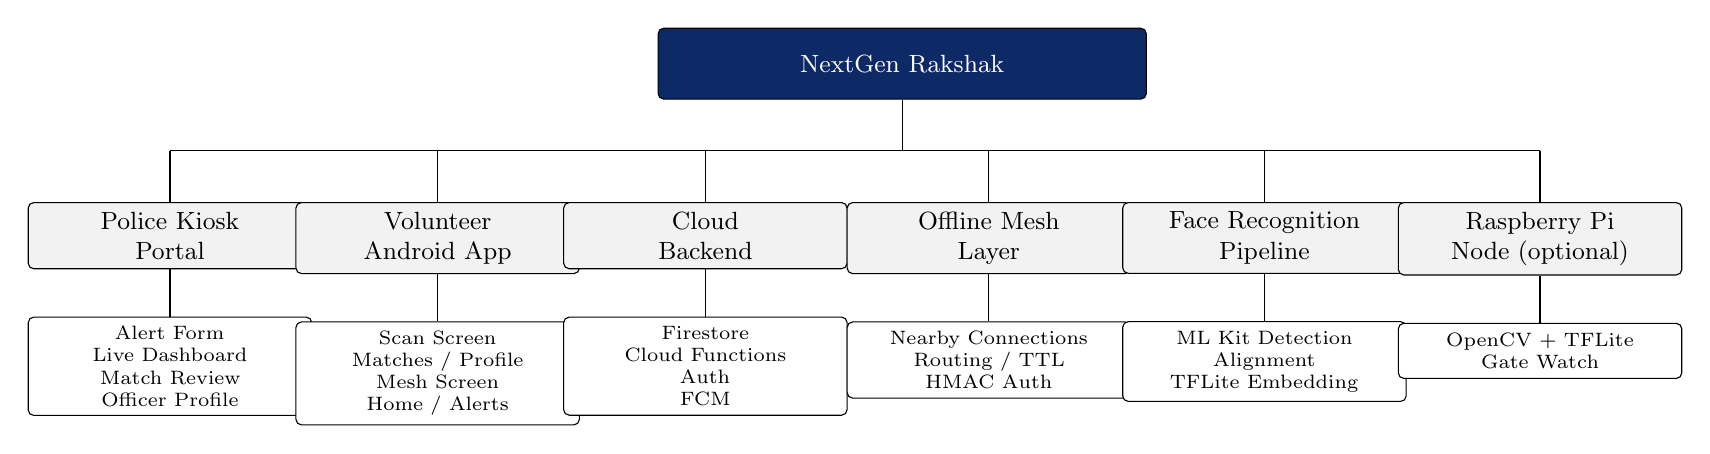
\begin{tikzpicture}[
  every node/.style={draw, rounded corners=2pt, align=center, font=\small},
  root/.style={fill=rakshaknavy, text=white, minimum width=6.2cm, minimum height=0.9cm},
  mod/.style={fill=lightgray, minimum width=3.6cm, minimum height=0.8cm},
  sub/.style={fill=white, minimum width=3.2cm, minimum height=0.7cm, font=\scriptsize},
  level distance=1.6cm
]
\node[root] (root) {NextGen Rakshak};

\node[mod, below=1.3cm of root, xshift=-9.3cm] (kiosk) {Police Kiosk\\Portal};
\node[mod, below=1.3cm of root, xshift=-5.9cm] (mobile) {Volunteer\\Android App};
\node[mod, below=1.3cm of root, xshift=-2.5cm] (cloud) {Cloud\\Backend};
\node[mod, below=1.3cm of root, xshift=1.1cm] (mesh) {Offline Mesh\\Layer};
\node[mod, below=1.3cm of root, xshift=4.6cm] (face) {Face Recognition\\Pipeline};
\node[mod, below=1.3cm of root, xshift=8.1cm] (pi) {Raspberry Pi\\Node (optional)};

% Orthogonal bus connector: one drop from root, one horizontal bus,
% then one clean vertical drop into each module -- no diagonal fan-in.
\coordinate (busA) at ($(root.south)+(0,-0.65)$);
\draw (root.south) -- (busA);
\draw ([xshift=-9.3cm]busA) -- ([xshift=8.1cm]busA);
\foreach \m/\x in {kiosk/-9.3cm, mobile/-5.9cm, cloud/-2.5cm, mesh/1.1cm, face/4.6cm, pi/8.1cm}
  \draw ([xshift=\x]busA) -- (\m.north);

\node[sub, below=0.6cm of kiosk, minimum width=3.6cm, text width=3.3cm] (k1)
  {Alert Form\\Live Dashboard\\Match Review\\Officer Profile};
\node[sub, below=0.6cm of mobile, minimum width=3.6cm, text width=3.3cm] (m1)
  {Scan Screen\\Matches / Profile\\Mesh Screen\\Home / Alerts};
\node[sub, below=0.6cm of cloud, minimum width=3.6cm, text width=3.3cm] (c1)
  {Firestore\\Cloud Functions\\Auth\\FCM};
\node[sub, below=0.6cm of mesh, minimum width=3.6cm, text width=3.3cm] (n1)
  {Nearby Connections\\Routing / TTL\\HMAC Auth};
\node[sub, below=0.6cm of face, minimum width=3.6cm, text width=3.3cm] (f1)
  {ML Kit Detection\\Alignment\\TFLite Embedding};
\node[sub, below=0.6cm of pi, minimum width=3.6cm, text width=3.3cm] (p1)
  {OpenCV + TFLite\\Gate Watch};

\foreach \pr/\ch in {kiosk/k1, mobile/m1, cloud/c1, mesh/n1, face/f1, pi/p1}
  \draw (\pr.south) -- (\ch.north);
\end{tikzpicture}%
}
\caption{System breakdown structure}
\label{fig:sbs}
\end{figure}

\section{Module Details}

\subsection{User}

\begin{table}[H]
\centering
\caption{User actors and their interaction with the system}
\begin{tabular}{|>{\raggedright\arraybackslash}p{3.6cm}|p{10.0cm}|}
\hline
\textbf{Actor} & \textbf{Role in the system} \\
\hline
Police Officer & Signs in to the kiosk (Google sign-in $\rightarrow$ \code{police} custom claim); files, tracks, and resolves alerts; reviews and dispatches volunteer-reported sightings. \\ \hline
Volunteer (Police, NCC, NGO, Community) & Signs in with Google on the mobile app; receives geofenced alerts; scans the crowd; visually confirms or dismisses a candidate match; carries the offline mesh when out of network range. \\ \hline
System (automated) & Cloud Functions execute unattended: computing the fallback embedding, broadcasting the geofenced push, purging biometric data on resolve, and expiring stale alerts. \\
\hline
\end{tabular}
\end{table}

\subsection{System Module}

\begin{table}[H]
\centering
\caption{Core system modules and their responsibility}
\begin{tabular}{|p{3.6cm}|p{10.0cm}|}
\hline
\textbf{Module} & \textbf{Responsibility} \\
\hline
Alert Management & Create, list, filter, and resolve missing-child alert records; store the case photo and structured details. \\ \hline
Face Detection \& Alignment & Locate faces in the live camera stream, reject non-frontal poses, and warp the face onto a canonical template before embedding. \\ \hline
Embedding \& Matching Engine & Compute a fixed-length face embedding on-device and score it against every active alert with cosine similarity. \\ \hline
Notification \& Geofencing & Compute which registered volunteers fall within the alert's geofence and dispatch a push notification through Firebase Cloud Messaging. \\ \hline
Offline Mesh Routing & Propagate alerts and confirmed sightings between devices with no internet, using TTL-bounded, authenticated, de-duplicated flooding. \\ \hline
Match Review \& Dispatch & Present a volunteer's confirmed sighting to the filing officer side-by-side with the original photo, and let the officer accept, dismiss, or dispatch. \\ \hline
Data Lifecycle / Privacy Purge & Delete the case photo and clear the stored embedding the moment a case is resolved or expires. \\
\hline
\end{tabular}
\end{table}

\section{Project Estimation}

\subsection{Estimation in KLOC}

Project size was estimated using an actual line count of hand-authored
source across the four components (auto-generated model schema files were
excluded, as they are not project-authored code).

\begin{table}[H]
\centering
\caption{Lines-of-code count by component}
\begin{tabular}{|p{4.6cm}|p{2.4cm}|p{2.4cm}|p{2.4cm}|}
\hline
\textbf{Component} & \textbf{Language} & \textbf{Files} & \textbf{LOC} \\
\hline
Volunteer Android app & Kotlin & 91 & 11{,}251 \\ \hline
Police kiosk web portal & TypeScript/TSX & 49 & 4{,}391 \\ \hline
Cloud Functions & TypeScript & 4 & 726 \\ \hline
Model tooling \& evaluation & Python & 9 & 1{,}662 \\
\hline
\textbf{Total} & & \textbf{153} & \textbf{18{,}030} \\
\hline
\end{tabular}
\end{table}

Total size $\approx$ \textbf{18.0 KLOC}.

\subsection{Efforts}

Applying the \textbf{Basic COCOMO} model \cite{cocomo} in \emph{Organic} mode (small,
experienced team, a well-understood problem domain -- appropriate for a
four-member student team building on documented platforms):

\[
E = a \cdot (\text{KLOC})^{b}, \qquad a = 2.4,\ b = 1.05
\]
\[
E = 2.4 \times (18.0)^{1.05} \approx 2.4 \times 20.85 \approx \textbf{50.0 person-months}
\]

\subsection{Development time in months}

\[
D = c \cdot (E)^{d}, \qquad c = 2.5,\ d = 0.38
\]
\[
D = 2.5 \times (50.0)^{0.38} \approx 2.5 \times 4.42 \approx \textbf{11.1 months}
\]

\subsection{Total Time Required for Project Development}

COCOMO's organic-mode estimate of $\approx$11 months reflects a
professionally staffed, production-hardened build. The team delivered a
feature-complete MVP against the objectives in \S1.4 within a compressed
academic timeline of approximately 8 weeks of active development (Phases~1--9,
Table~\ref{tab:schedule}), scoped deliberately as a validated prototype
rather than a production-hardened system -- the gap between the two
estimates is consistent with, and explained by, the reduced scope (no
formal QA cycle, a single target platform, and a small, pre-defined feature
set) appropriate to a final-year academic deliverable.

\subsection{Number of Developers (N)}

\[
N = \frac{E}{D} = \frac{50.0}{11.1} \approx \textbf{4.5 people}
\]

This COCOMO-derived average staffing figure of $\approx$4--5 people aligns
closely with the actual team size of four, supporting the estimation
model's applicability to this project despite the compressed academic
schedule.

% ============================================================================
%  CHAPTER 4 -- SYSTEM ANALYSIS
% ============================================================================
\chapter{System Analysis}

\section{Project Scheduling and Tracking}

\subsection{Project Work and Breakdown Structure (Analysis)}

The analysis phase (Phases 1--2 of the project schedule) decomposed the
problem into requirement gathering and system design work packages before
any code was written.

\begin{figure}[H]
\centering
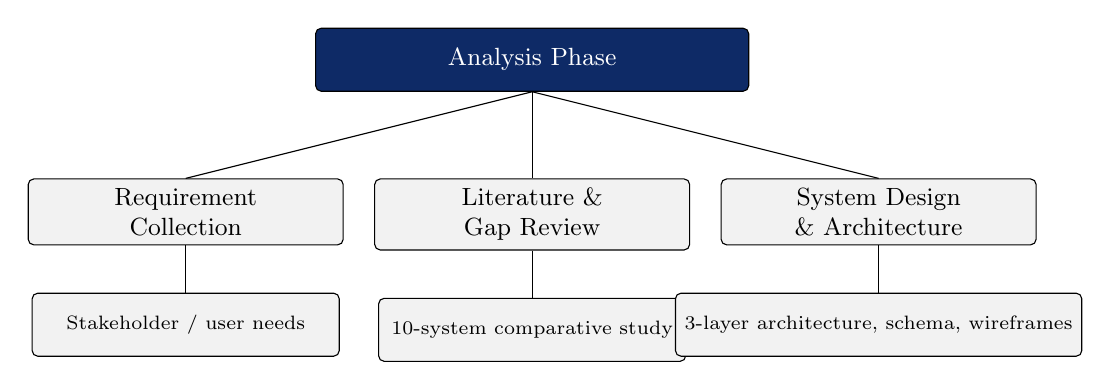
\begin{tikzpicture}[
  every node/.style={draw, rounded corners=2pt, align=center, font=\small, fill=lightgray, minimum height=0.8cm},
  root/.style={fill=rakshaknavy, text=white, minimum width=5.5cm}
]
\node[root] (r) {Analysis Phase};
\node[below=1.1cm of r, xshift=-4.4cm, minimum width=4cm] (a) {Requirement\\Collection};
\node[below=1.1cm of r, minimum width=4cm] (b) {Literature \&\\Gap Review};
\node[below=1.1cm of r, xshift=4.4cm, minimum width=4cm] (c) {System Design\\\& Architecture};
\draw (r.south) -- (a.north); \draw (r.south) -- (b.north); \draw (r.south) -- (c.north);

\node[below=0.6cm of a, minimum width=3.9cm, font=\scriptsize] (a1) {Stakeholder / user needs};
\node[below=0.6cm of b, minimum width=3.9cm, font=\scriptsize] (b1) {10-system comparative study};
\node[below=0.6cm of c, minimum width=3.9cm, font=\scriptsize] (c1) {3-layer architecture, schema, wireframes};
\draw (a.south) -- (a1.north); \draw (b.south) -- (b1.north); \draw (c.south) -- (c1.north);
\end{tikzpicture}
\caption{Work breakdown structure -- Analysis phase}
\end{figure}

\subsection{Version Control and Commit History}
\label{sec:vcs-history}

The entire project -- all three components, the Cloud Functions, the model
scripts, and every weekly report -- is tracked in a single public Git
repository hosted on GitHub at
\url{https://github.com/ByteNinjaSmit/NextGen-Rakshak}. The commit history
is the project's actual, unedited build log: 64 commits from the first
commit on 21 July 2026 to the last on 13 September 2026, an unbroken
$\sim$8-week record of the incremental process described in \S3.1.

\begin{table}[H]
\centering
\caption{Commit authorship}
\begin{tabular}{|p{5.4cm}|p{2.5cm}|p{5.0cm}|}
\hline
\textbf{Author} & \textbf{Commits} & \textbf{Track (Table~\ref{tab:ownership})} \\
\hline
Smitraj Bankar (\texttt{ByteNinjaSmit}) & 53 & Architecture, ML pipeline, mesh, Cloud Functions, integration \\ \hline
AtharvaNarkhede1 & 10 & UI/UX, web portal styling, integration testing \\ \hline
Vedant Dhadge & 1 & Android/Firebase integration \\
\hline
\end{tabular}
\end{table}

\noindent Two feature branches, \texttt{AndriodUI} and \texttt{WebPortalUI},
were split off \texttt{main} for the Week~5--6 UI overhaul and merged back
through reviewed pull requests (PR~\#1 merged \texttt{WebPortalUI} on
12~August 2026) -- the branch discipline identified as a gap in the Week~4
risk review (R10, \S5.1) was adopted from that point on, rather than left
as an unaddressed finding. Commit subjects follow the Conventional Commits
convention (\texttt{feat:}, \texttt{fix:}, \texttt{docs:}, \texttt{build:},
\texttt{chore:}), which is what makes the table below possible to produce
directly from \texttt{git log} rather than from memory.

\begin{longtable}{|p{1.7cm}|p{1.5cm}|p{9.5cm}|}
\caption{Representative commits, in order (full history: \texttt{git log} on \texttt{main})}
\label{tab:commits}\\
\hline
\textbf{Date} & \textbf{Hash} & \textbf{Subject} \\
\hline
\endfirsthead
\hline
\textbf{Date} & \textbf{Hash} & \textbf{Subject} \\
\hline
\endhead
21 Jul & \texttt{2211d78} & feat: initial commit -- NextGen Rakshak lost-child recovery system \\ \hline
21 Jul & \texttt{022ff83} & feat: side-by-side match confirmation, match haptics, photo purge on resolve \\ \hline
22 Jul & \texttt{e727b69} & feat: working MobileFaceNet pipeline -- SavedModel on server, tflite on device \\ \hline
22 Jul & \texttt{f9128a9} & feat: lower match threshold to 0.55 from measurement, add Week 3 documentation \\ \hline
22 Jul & \texttt{a96c7b3} & fix: gate the police kiosk on a police claim, not merely being signed in \\ \hline
22 Jul & \texttt{998307b} & build: switch to LiteRT and Kotlin 2.3 so all 64-bit libraries are 16\,KB aligned \\ \hline
29 Jul & \texttt{f80f30e} & feat: self-register kiosk officers, smooth login/logout popup UX \\ \hline
30 Jul & \texttt{0f40a9d} & feat: mesh case-closure, hardened match writes, offline fixes \\ \hline
01 Aug & \texttt{b5a6f57} & feat: dashboard active alerts/live match update, new alert form fields \\ \hline
12 Aug & \texttt{67cb647} & Merge pull request \#1 from \texttt{ByteNinjaSmit/WebPortalUI} \\ \hline
13 Aug & \texttt{9e4fc3f} & feat: kiosk notification bell with FCM match push \\ \hline
13 Aug & \texttt{136a28b} & chore: upgrade functions to Node 22 and firebase-functions v7 \\ \hline
15 Aug & \texttt{0d35a5c} & feat: implement MatchesScreen, MatchConfirmation dialog, updated UI themes \\ \hline
23 Aug & \texttt{d741609} & android face done \\ \hline
02 Sep & \texttt{ef3998f} & feat: face-match accuracy -- alignment, multi-frame fusion, quality gate \\ \hline
02 Sep & \texttt{8a3dc4a} & feat: offline mesh -- advanced pass (thumbnail, HMAC, foreground service, persistence) \\ \hline
02 Sep & \texttt{4d2f9a8} & fix: location \& geofencing review -- rules regression + fail-open hardening \\ \hline
05 Sep & \texttt{fad33c5} & feat: simplify auth to Google-only, enforce system roles, camera switch \\ \hline
07 Sep & \texttt{bb0f829} & fix: restore live face matching -- model deadlock, geometry drift, track pollution \\ \hline
13 Sep & \texttt{8a3d32a} & feat(mobile): SIM-backed contact number, Google avatar, live mesh screen \\ \hline
13 Sep & \texttt{dd37ec8} & feat(webportal): interactive dashboard stats, pagination/filters, layout scroll fix \\ \hline
13 Sep & \texttt{33062cf} & fix: fall back to placeholder icon when alert photo fails to load \\
\hline
\end{longtable}

The trajectory the log records matches the incremental plan exactly rather
than being reconstructed after the fact: the online path (kiosk, auth,
first face pipeline) lands in the first two weeks; the threshold revision
from an assumed 0.75 to a measured 0.55 (\texttt{f9128a9}) and the switch
from anonymous to Google sign-in (\texttt{9e73b85}) are both mid-project
corrections driven by evidence, not planning; the
mesh layer's authentication, thumbnail, and gateway-routing work
(\texttt{8a3dc4a}, \texttt{6aed293}) lands in a single dense week once the
online path was stable; and the final fortnight (\texttt{bb0f829} onward)
is entirely defect-fix and polish commits against real-device testing,
exactly as the Week~7--8 schedule in Table~\ref{tab:schedule} intended.

\subsection{Weekly Progress Log (Guide-Assessed)}
\label{sec:weekly-log}

Independently of the phase table above, the department's weekly assessment
process tracked the team against a 10-week guide-reviewed log, one signed
form per week (reproduced in full, with each week's guide remark, in
\texttt{docs/weekly-reports/}). \textbf{Both records agree on the same
conclusion: the system
itself -- both applications, the cloud backend, and the offline mesh --
was fully built, integrated, and tested within these 10 weeks, with final
integration complete by 15 September 2026.} Table~\ref{tab:schedule}'s
later phases (research-paper drafting, copyright filing) are
post-completion academic output, not outstanding system work; they are
tracked separately in \S9.2.

\small
\begin{longtable}{|p{0.9cm}|p{2.1cm}|p{10.7cm}|}
\caption{Weekly guide-assessment log, Week 1--10 (5 July -- 15 September 2026), by member responsibility (Table~\ref{tab:ownership})}
\label{tab:weeklylog}\\
\hline
\textbf{Wk} & \textbf{Dates} & \textbf{Work done, by member} \\
\hline
\endfirsthead
\hline
\textbf{Wk} & \textbf{Dates} & \textbf{Work done, by member} \\
\hline
\endhead
1 & 05--11 Jul &
\textbf{Bankar:} reviewed MobileFaceNet/TFLite and ML Kit documentation for on-device recognition feasibility.\newline
\textbf{Bhakare:} reviewed TrackChild, Khoya-Paya, and ReUnite, establishing the reactive/server-dependent research gap.\newline
\textbf{Narkhede:} compiled the NCRB missing-children figures and the Supreme Court's golden-hour observation to frame the problem.\newline
\textbf{Dhadge:} studied the Nearby Connections API for offline peer-to-peer feasibility. \\ \hline
2 & 12--18 Jul &
\textbf{Bankar:} drafted the three-layer (Cloud/Edge/Mesh) architecture diagram and finalised the technology stack.\newline
\textbf{Bhakare:} designed the inter-component interaction flow (kiosk $\to$ FCM $\to$ volunteer $\to$ mesh) and communication protocols.\newline
\textbf{Narkhede:} designed UI wireframes for the kiosk and Android app.\newline
\textbf{Dhadge:} planned the Firestore schema (\code{alerts}, \code{volunteers}, \code{matches}, roles). \\ \hline
3 & 19--25 Jul &
\textbf{Bankar:} studied Firebase Cloud Functions for embedding computation and alert-broadcast logic.\newline
\textbf{Bhakare:} studied MobileFaceNet/TFLite implementation and model validation (quantisation, accuracy evaluation).\newline
\textbf{Narkhede:} designed UI wireframes for the kiosk and Android app screens.\newline
\textbf{Dhadge:} studied Firebase Authentication and role-based access control. \\ \hline
4 & 26 Jul--01 Aug &
\textbf{Bankar:} tested Cloud Functions and Firestore operations; deployed the kiosk to Vercel for iterative testing.\newline
\textbf{Bhakare:} studied the Next.js framework -- routing, project structure, and setup.\newline
\textbf{Narkhede:} implemented frontend UI colour changes, dashboard alerts/live-match updates, the new alert form, and login/register pages.\newline
\textbf{Dhadge:} studied Android fundamentals, set up the dev environment, and scaffolded the bare-bones volunteer app. \\ \hline
5 & 02--08 Aug &
\textbf{Bankar:} implemented Cloud Functions (embedding, FCM broadcast, match processing) with Firestore triggers; deployed and verified.\newline
\textbf{Bhakare:} studied Next.js App/API routes, server/client components, and middleware; reviewed the implemented pages.\newline
\textbf{Narkhede:} completed the dashboard UI/UX with Firebase integration -- login/register, live updates, profile, validation, responsive layout.\newline
\textbf{Dhadge:} implemented runtime permissions (camera, location, Nearby), the scan-screen UI, and navigation. \\ \hline
6 & 09--15 Aug &
\textbf{Bankar:} redeployed Cloud Functions on the upgraded Node runtime; sourced MobileFaceNet weights and built the conversion scripts.\newline
\textbf{Bhakare:} measured recognition accuracy on 36 labelled pairs using the quantised model (see \S\ref{sec:threshold-measurement} for the figures carried into this report).\newline
\textbf{Narkhede:} ran the Android/web cross-platform consistency pass and UI language alignment.\newline
\textbf{Dhadge:} scoped the TPEB paper and tested the Android build on the UI branch. \\ \hline
7 & 16--22 Aug &
\textbf{Bankar:} optimised Cloud Functions (cold-start, response time) and redeployed.\newline
\textbf{Bhakare:} finalised the MobileFaceNet \code{.tflite} integration, tuned the threshold against the measured pairs, and optimised for low-end devices.\newline
\textbf{Narkhede:} completed kiosk/Android sync, the role-based dashboard, and profile validation.\newline
\textbf{Dhadge:} implemented the offline mesh layer (Nearby Connections, multi-hop store-and-forward) with working peer discovery. \\ \hline
8 & 23--29 Aug &
\textbf{Bankar:} ran backend load and Firestore-rules testing, and fixed FCM broadcast reliability issues.\newline
\textbf{Bhakare:} tested on-device recognition accuracy under varied lighting.\newline
\textbf{Narkhede:} completed full kiosk integration testing (auth, dashboard, alerts, profile, responsive/cross-browser) and fixed UI inconsistencies.\newline
\textbf{Dhadge:} ran Android instrumentation testing, the offline-mesh field test, and battery/network profiling. \\ \hline
9 & 30 Aug--05 Sep &
\textbf{Bankar:} finalised the production deployment (Vercel + Firebase) with a Firestore backup and backend documentation.\newline
\textbf{Bhakare:} finalised the accuracy write-up, model optimisation, and inference benchmarking documentation.\newline
\textbf{Narkhede:} completed final UI/UX polish, the user manual, presentation slides, and demo-flow verification.\newline
\textbf{Dhadge:} built the final release APK, ran final device testing, and contributed to the TPEB paper draft. \\ \hline
10 & 06--15 Sep &
\textbf{Bankar:} diagnosed and fixed the two mesh reconnect-stability defects found in the 3-device field trial (\S\ref{sec:field-trial}) -- the missing runtime \code{NEARBY\_WIFI\_DEVICES} request and the \code{onEndpointLost} miswiring (\S\ref{sec:mesh-reconnect}) -- and the TFLite interpreter concurrency deadlock (\S\ref{sec:concurrency-safety}).\newline
\textbf{Bhakare:} shipped the kiosk's interactive dashboard -- clickable stat tiles, match-status chart, top-volunteers leaderboard -- with pagination/filters and a layout scroll fix.\newline
\textbf{Narkhede:} verified the field-trial fixes end-to-end and ran final UI/UX validation across the redesigned mesh and dashboard screens.\newline
\textbf{Dhadge:} shipped the SIM-backed volunteer contact number (dual-SIM picker), Google-avatar profile identity, and the live mesh-visualisation screen. System declared feature-complete and frozen on 15 September 2026 (Table~\ref{tab:commits}). \\
\hline
\end{longtable}
\normalsize

Every item in Week 10 traces to a specific commit in Table~\ref{tab:commits}
(\texttt{bb0f829} through \texttt{33062cf}); nothing in this final week is a
desk-review finding -- all of it, including the two mesh defects, surfaced
only once the finished system was exercised end-to-end on real, physically
separate devices, which is precisely why it took a dedicated closing week
rather than being caught earlier.

\section{Project Work Breakdown Structure (Implementation)}

The implementation phase (Phases 3--9) decomposed into three parallel
development sprints followed by integration, hardening, and deployment.

\begin{figure}[H]
\centering
\resizebox{\textwidth}{!}{%
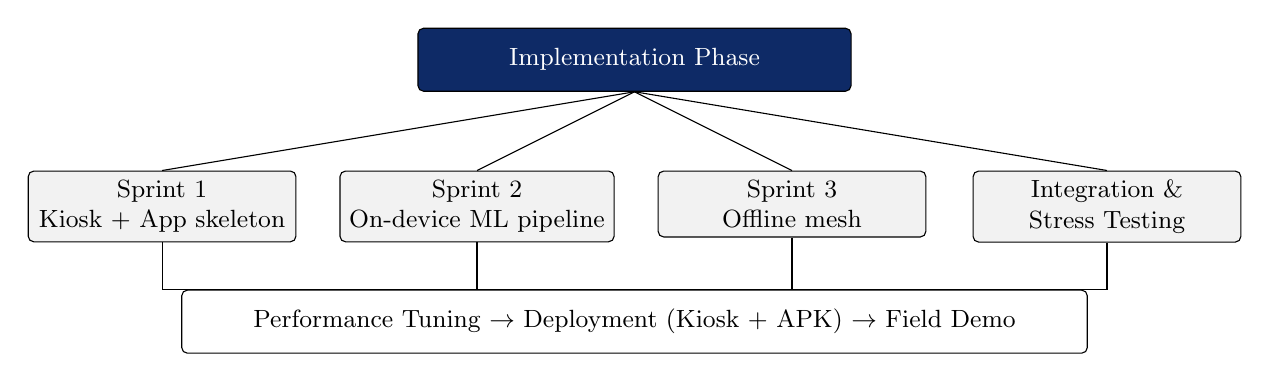
\begin{tikzpicture}[
  every node/.style={draw, rounded corners=2pt, align=center, font=\small, fill=lightgray, minimum height=0.8cm},
  root/.style={fill=rakshaknavy, text=white, minimum width=5.5cm}
]
\node[root] (r) {Implementation Phase};
\node[below=1.0cm of r, xshift=-6.0cm, minimum width=3.4cm] (a) {Sprint 1\\Kiosk + App skeleton};
\node[below=1.0cm of r, xshift=-2.0cm, minimum width=3.4cm] (b) {Sprint 2\\On-device ML pipeline};
\node[below=1.0cm of r, xshift=2.0cm, minimum width=3.4cm] (c) {Sprint 3\\Offline mesh};
\node[below=1.0cm of r, xshift=6.0cm, minimum width=3.4cm] (d) {Integration \&\\Stress Testing};
\foreach \n in {a,b,c,d} \draw (r.south) -- (\n.north);

\node[below=0.6cm of b, xshift=2.0cm, minimum width=11.5cm, fill=white, font=\small] (e) {Performance Tuning $\rightarrow$ Deployment (Kiosk + APK) $\rightarrow$ Field Demo};
\draw (a.south) |- (e.north); \draw (b.south) |- (e.north);
\draw (c.south) |- (e.north); \draw (d.south) |- (e.north);
\end{tikzpicture}%
}
\caption{Work breakdown structure -- Implementation phase}
\end{figure}

\section{Task Identification}

\subsection{Ownership and Responsibility (as filed in the Project Proposal)}
\label{sec:ownership}

Task ownership was fixed at the proposal stage, before any code was
written, and held for the life of the project -- every week in the 10-week
log (Table~\ref{tab:weeklylog}) is an instance of the same four-way split
defined here.

\begin{table}[H]
\centering
\caption{Task ownership and expected contribution, as filed in the project proposal}
\label{tab:ownership}
\begin{tabular}{|p{2.7cm}|p{8.0cm}|p{2.3cm}|}
\hline
\textbf{Student} & \textbf{Responsibility} & \textbf{Contribution} \\
\hline
Bankar Smitraj Dinkar (09) &
Overall project lead and system architect -- owns the end-to-end
architecture (Cloud/Edge/Mesh layers), the backend (Firebase Cloud
Functions, Firestore schema), on-device ML pipeline integration (ML Kit +
MobileFaceNet/TFLite), the offline mesh implementation (Nearby Connections
+ custom routing), cross-component integration, and final report/research
paper/patent-filing coordination. &
$\sim$40\% -- First Author \\
\hline
Bhakare Tanishka Sharad (11) &
Web portal development -- builds the Police Kiosk Portal in
Next.js/React/TypeScript/Tailwind CSS, including the alert-creation form,
live matches dashboard, and Firebase integration (Auth, Firestore
listeners). &
$\sim$20\% -- Co-Author \\
\hline
Narkhede Atharva Anantkumar (94) &
UI/UX design across both platforms and QA -- designs wireframes (Figma)
for the Police Kiosk Portal and Volunteer Android App interfaces, and
leads functional/integration testing across the system (multi-device
offline-mesh tests, multi-alert stress tests, UI/UX validation). &
$\sim$20\% -- Co-Author \\
\hline
Dhadge Vedant Sanjay (34) &
Android application development and Firebase integration -- builds the
Volunteer Android App (Kotlin, Jetpack Compose, CameraX) and wires it to
Firebase (Authentication, Firestore sync, Cloud Messaging) for alert
receipt and match reporting. &
$\sim$20\% -- Co-Author \\
\hline
\end{tabular}
\end{table}

\subsection{Project Schedule}

Table~\ref{tab:schedule} lists the twelve project phases as planned and
tracked from the project's governance record, spanning requirement
collection through report writing, performance tuning, deployment, field
demonstration, and copyright filing preparation.

\section{Project Table and Time-line Chart}

\subsection{Project Schedule Time}

\begin{table}[H]
\centering
\caption{Project phase schedule}
\label{tab:schedule}
\begin{tabular}{|p{1.2cm}|p{7.2cm}|p{2.1cm}|p{2.5cm}|}
\hline
\textbf{Phase} & \textbf{Milestone} & \textbf{Duration} & \textbf{Start} \\
\hline
1  & Requirement collection, literature review, synopsis finalisation & 2 weeks & 11 Aug 2026 \\ \hline
2  & System design: three-layer architecture, schema, API contracts, wireframes & 2 weeks & 12 Aug 2026 \\ \hline
3  & Dev Sprint 1: Police kiosk portal + volunteer app skeleton & 2 weeks & 13 Aug 2026 \\ \hline
4  & Dev Sprint 2: On-device ML pipeline (detection, embedding, matching) & 2 weeks & 27 Aug 2026 \\ \hline
5  & Dev Sprint 3: Offline mesh (routing, TTL, dedup) + optional Pi node & 1 week & 03 Sep 2026 \\ \hline
6  & Integration, multi-alert stress test, 5--10 device mesh test, bug-fix & 1 week & 10 Sep 2026 \\ \hline
7  & Final project report writing \& documentation & 2 weeks & 24 Sep 2026 \\ \hline
8  & Performance optimisation: threshold calibration, latency, battery tuning & 2 weeks & 08 Oct 2026 \\ \hline
9  & Deployment: hosted kiosk, sideloaded volunteer APK, optional Pi field setup & 2 weeks & 22 Oct 2026 \\ \hline
10 & Field test / pilot demonstration with 5--10 volunteers & 3 weeks & 12 Nov 2026 \\ \hline
11 & Research-paper drafting from field-test and benchmark results & 3 weeks & 03 Dec 2026 \\ \hline
12 & Patent / copyright filing preparation and submission & 4 weeks & 15 Jan 2027 \\
\hline
\end{tabular}
\end{table}

\subsection{Time-Line Chart}

\begin{figure}[H]
\centering
\resizebox{\textwidth}{!}{%
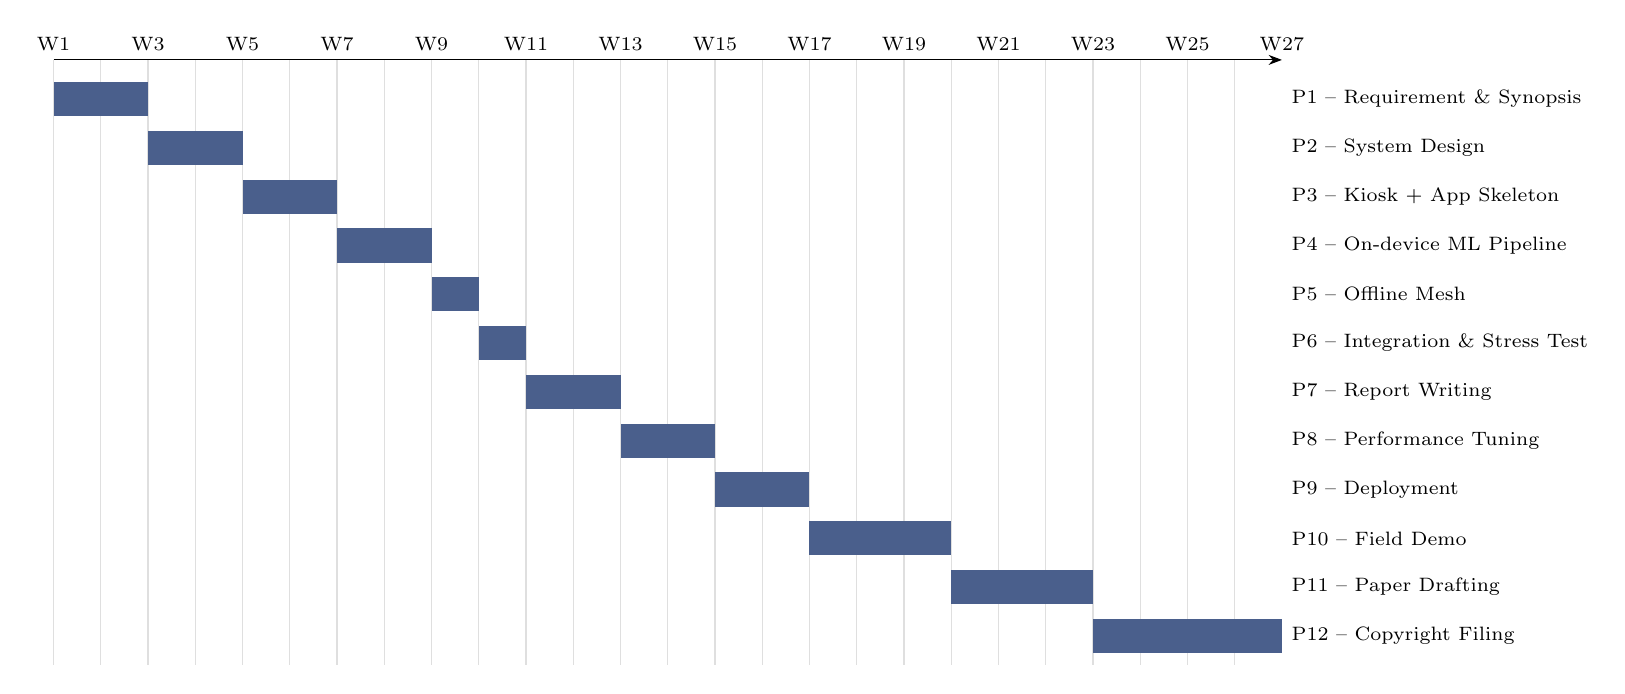
\begin{tikzpicture}[x=0.6cm, y=-0.62cm, font=\scriptsize]
  % gridlines
  \foreach \w in {1,...,26}
    \draw[gray!25] (\w,-0.3) -- (\w,12.1);
  % phase bars: (start week, length in weeks, row, label)
  \fill[rakshaknavy!75] (1,0.15)  rectangle ++(2,0.7);
  \node[anchor=west] at (27,0.5)  {P1 -- Requirement \& Synopsis};
  \fill[rakshaknavy!75] (3,1.15)  rectangle ++(2,0.7);
  \node[anchor=west] at (27,1.5)  {P2 -- System Design};
  \fill[rakshaknavy!75] (5,2.15)  rectangle ++(2,0.7);
  \node[anchor=west] at (27,2.5)  {P3 -- Kiosk + App Skeleton};
  \fill[rakshaknavy!75] (7,3.15)  rectangle ++(2,0.7);
  \node[anchor=west] at (27,3.5)  {P4 -- On-device ML Pipeline};
  \fill[rakshaknavy!75] (9,4.15)  rectangle ++(1,0.7);
  \node[anchor=west] at (27,4.5)  {P5 -- Offline Mesh};
  \fill[rakshaknavy!75] (10,5.15) rectangle ++(1,0.7);
  \node[anchor=west] at (27,5.5)  {P6 -- Integration \& Stress Test};
  \fill[rakshaknavy!75] (11,6.15) rectangle ++(2,0.7);
  \node[anchor=west] at (27,6.5)  {P7 -- Report Writing};
  \fill[rakshaknavy!75] (13,7.15) rectangle ++(2,0.7);
  \node[anchor=west] at (27,7.5)  {P8 -- Performance Tuning};
  \fill[rakshaknavy!75] (15,8.15) rectangle ++(2,0.7);
  \node[anchor=west] at (27,8.5)  {P9 -- Deployment};
  \fill[rakshaknavy!75] (17,9.15) rectangle ++(3,0.7);
  \node[anchor=west] at (27,9.5)  {P10 -- Field Demo};
  \fill[rakshaknavy!75] (20,10.15) rectangle ++(3,0.7);
  \node[anchor=west] at (27,10.5) {P11 -- Paper Drafting};
  \fill[rakshaknavy!75] (23,11.15) rectangle ++(4,0.7);
  \node[anchor=west] at (27,11.5) {P12 -- Copyright Filing};
  % week axis
  \draw[-{Stealth}] (1,-0.3) -- (27,-0.3);
  \foreach \w in {1,3,5,7,9,11,13,15,17,19,21,23,25,27}
    \node[above] at (\w,-0.3) {W\w};
\end{tikzpicture}%
}
\caption{Project time-line chart (weeks from Phase 1 start, 11 Aug 2026)}
\end{figure}

\section{Analysis Modeling}

\subsection{Behavioral Modeling}

\paragraph{Use Case Diagram.}

\begin{figure}[H]
\centering
\resizebox{\textwidth}{!}{%
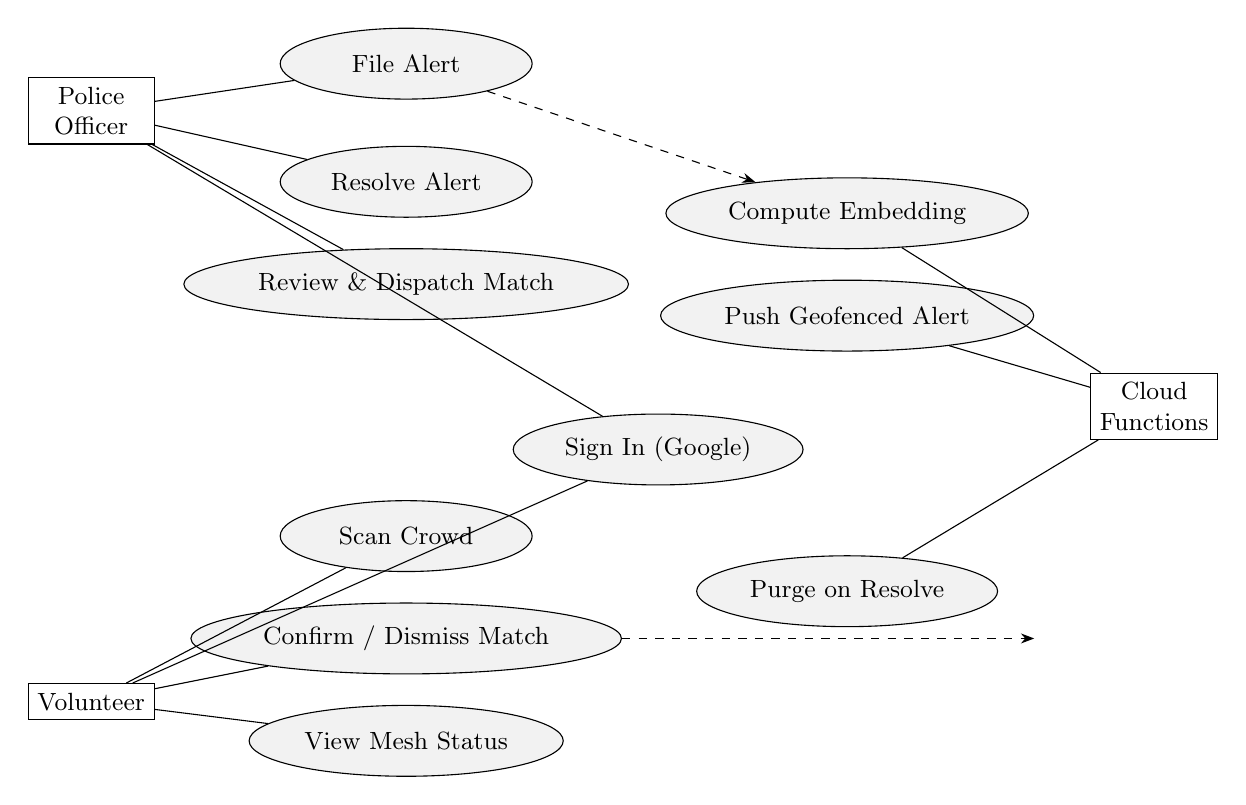
\begin{tikzpicture}[
  actor/.style={draw, minimum width=1.6cm, align=center, font=\small},
  usecase/.style={draw, ellipse, minimum width=3.2cm, minimum height=0.9cm, align=center, font=\small, fill=lightgray},
  >=Stealth
]
\node[actor] (officer) at (0,0) {Police\\Officer};
\node[actor] (vol) at (0,-7.5) {Volunteer};
\node[actor] (sys) at (13.5,-3.75) {Cloud\\Functions};

\node[usecase] (uc1) at (4,0.6)   {File Alert};
\node[usecase] (uc2) at (4,-0.9)  {Resolve Alert};
\node[usecase] (uc3) at (4,-2.2)  {Review \& Dispatch Match};
\node[usecase] (uc4) at (7.2,-4.3) {Sign In (Google)};
\node[usecase] (uc5) at (4,-5.4)  {Scan Crowd};
\node[usecase] (uc6) at (4,-6.7)  {Confirm / Dismiss Match};
\node[usecase] (uc7) at (4,-8.0)  {View Mesh Status};
\node[usecase] (uc8) at (9.6,-1.3) {Compute Embedding};
\node[usecase] (uc9) at (9.6,-2.6) {Push Geofenced Alert};
\node[usecase] (uc10) at (9.6,-6.1) {Purge on Resolve};

\draw (officer) -- (uc1); \draw (officer) -- (uc2); \draw (officer) -- (uc3); \draw (officer) -- (uc4);
\draw (vol) -- (uc4); \draw (vol) -- (uc5); \draw (vol) -- (uc6); \draw (vol) -- (uc7);
\draw[dashed,->] (uc1) -- (uc8);
\draw (sys) -- (uc8); \draw (sys) -- (uc9); \draw (sys) -- (uc10);
\draw[dashed,->] (uc6) -- (uc9.east |- uc6);
\end{tikzpicture}%
}
\caption{Use case diagram -- Police Officer, Volunteer, and Cloud Functions}
\end{figure}

\paragraph{Activity Diagram -- Alert-to-Match Flow.}

\begin{figure}[H]
\centering
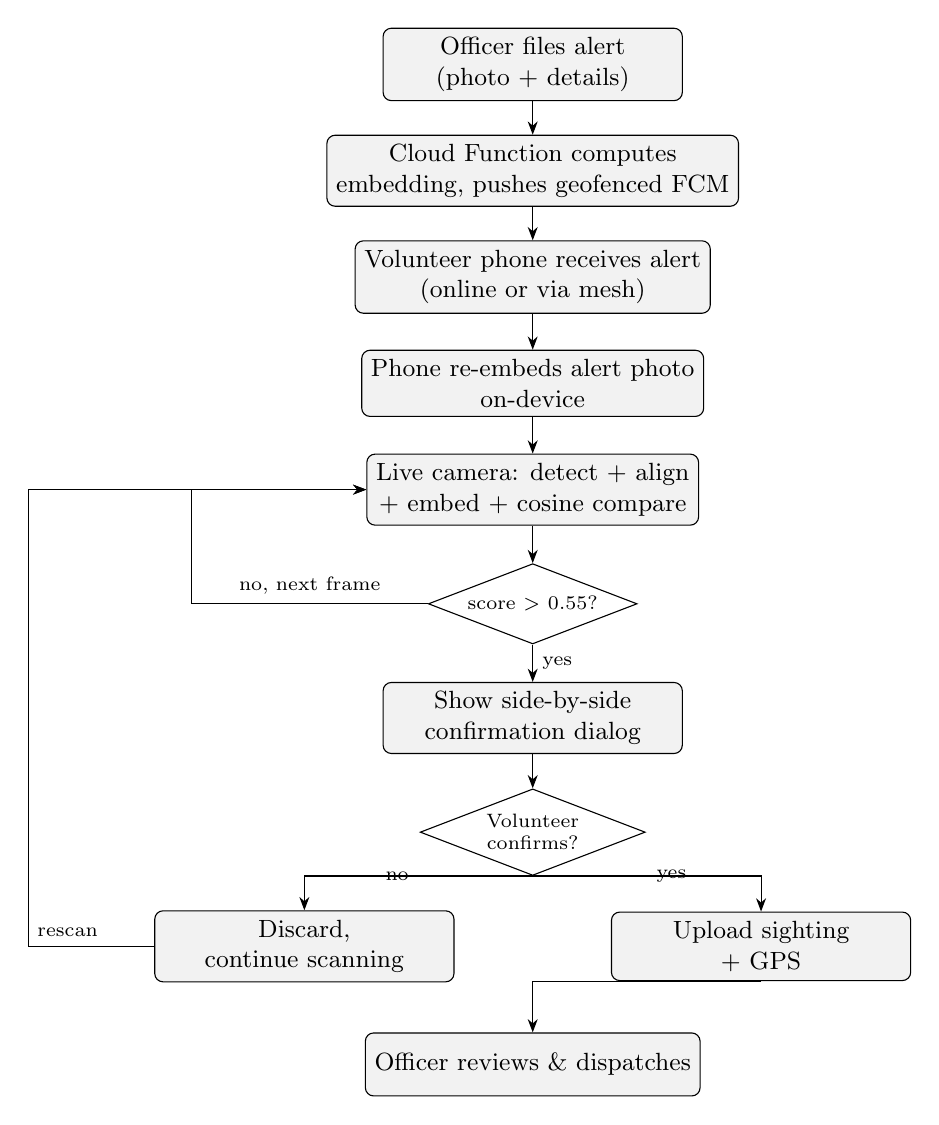
\begin{tikzpicture}[
  act/.style={draw, rounded corners=3pt, fill=lightgray, minimum width=3.8cm, minimum height=0.8cm, align=center, font=\small},
  dec/.style={draw, diamond, aspect=2.6, fill=white, align=center, font=\scriptsize, inner sep=2pt},
  >=Stealth
]
\node[act] (a1) at (0,0)      {Officer files alert\\(photo + details)};
\node[act] (a2) at (0,-1.35)  {Cloud Function computes\\embedding, pushes geofenced FCM};
\node[act] (a3) at (0,-2.70)  {Volunteer phone receives alert\\(online or via mesh)};
\node[act] (a4) at (0,-4.05)  {Phone re-embeds alert photo\\on-device};
\node[act] (a5) at (0,-5.40)  {Live camera: detect + align\\+ embed + cosine compare};
\node[dec] (d1) at (0,-6.85)  {score $>$ 0.55?};
\node[act] (a6) at (0,-8.30)  {Show side-by-side\\confirmation dialog};
\node[dec] (d2) at (0,-9.75)  {Volunteer\\confirms?};
\node[act] (a7) at (-2.9,-11.2) {Discard,\\continue scanning};
\node[act] (a8) at (2.9,-11.2)  {Upload sighting\\+ GPS};
\node[act] (a9) at (0,-12.7)    {Officer reviews \& dispatches};

% main spine -- straight verticals, all boxes share x=0
\draw[->] (a1)--(a2); \draw[->] (a2)--(a3); \draw[->] (a3)--(a4);
\draw[->] (a4)--(a5); \draw[->] (a5)--(d1);
\draw[->] (d1) -- node[right, font=\scriptsize]{yes} (a6);
\draw[->] (a6)--(d2);

% "no" feedback loop from the threshold check -- short stub out of d1,
% labelled right next to its source, then a clean drop into a5's side
\draw (d1.west) -- ++(-3.0,0) coordinate (noFb);
\draw[->] (noFb) |- (a5.west);
\node[font=\scriptsize, above] at ($(d1.west)!0.5!(noFb)$) {no, next frame};

% decision fork into discard / upload -- straight elbow from d2, no
% manual pre-drop, so the vertical segment is real and the arrow
% enters each box from above rather than side-on
\draw[->] (d2.south) -| node[near start,left,font=\scriptsize]{no} (a7.north);
\draw[->] (d2.south) -| node[near start,right,font=\scriptsize]{yes} (a8.north);

% discard rejoins the scan loop -- own stub, own label, far enough left
% and far enough below the "no, next frame" label that neither collides
\draw (a7.west) -- ++(-1.6,0) coordinate (discardFb);
\draw[->] (discardFb) |- (a5.west);
\node[font=\scriptsize, above, xshift=-0.3cm] at ($(a7.west)!0.5!(discardFb)$) {rescan};

% confirmed upload proceeds to dispatch -- clean elbow into the top of a9
\draw[->] (a8.south) -| (a9.north);
\end{tikzpicture}
\caption{Activity diagram -- alert filing through confirmed sighting}
\end{figure}

\paragraph{Sequence Diagram -- Confirmed Match (Online Path).}

\begin{figure}[H]
\centering
\resizebox{\textwidth}{!}{%
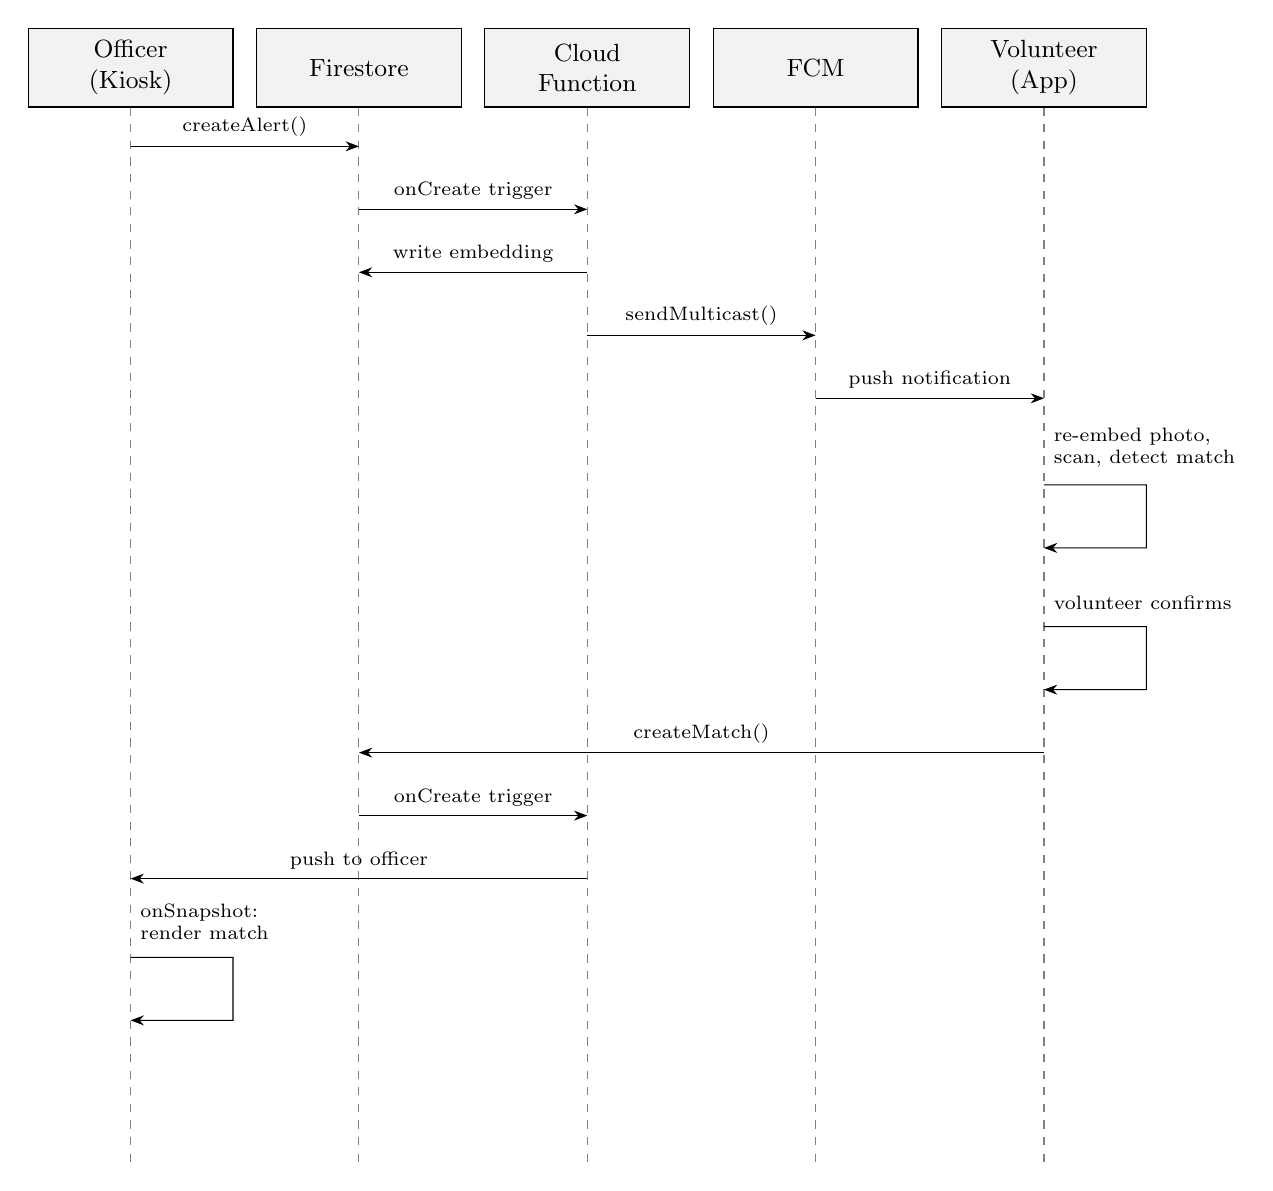
\begin{tikzpicture}[
  font=\small, >=Stealth,
  lifeline/.style={draw, dashed, gray},
  actorbox/.style={draw, fill=lightgray, align=center, minimum width=2.6cm, minimum height=1.0cm},
  msg/.style={->, >=Stealth},
  selfmsg/.style={->, >=Stealth}
]
% -- Five actor lifeline headers, each its own box, evenly spaced.
\node[actorbox] (h0) at (0,0)     {Officer\\(Kiosk)};
\node[actorbox] (h1) at (2.9,0)   {Firestore};
\node[actorbox] (h2) at (5.8,0)   {Cloud\\Function};
\node[actorbox] (h3) at (8.7,0)   {FCM};
\node[actorbox] (h4) at (11.6,0)  {Volunteer\\(App)};
\foreach \h in {h0,h1,h2,h3,h4}
  \draw[lifeline] (\h.south) -- ++(0,-13.4);

% -- Messages, one clean row each, consistent 0.8cm rhythm.
\draw[msg] (0,-1.0)   -- node[above,font=\scriptsize]{createAlert()}      (2.9,-1.0);
\draw[msg] (2.9,-1.8) -- node[above,font=\scriptsize]{onCreate trigger}   (5.8,-1.8);
\draw[msg] (5.8,-2.6) -- node[above,font=\scriptsize]{write embedding}    (2.9,-2.6);
\draw[msg] (5.8,-3.4) -- node[above,font=\scriptsize]{sendMulticast()}    (8.7,-3.4);
\draw[msg] (8.7,-4.2) -- node[above,font=\scriptsize]{push notification}  (11.6,-4.2);

% -- Self-message: volunteer phone re-embeds and scans (proper UML loop,
%    label sits clear ABOVE the loop's top line, never crossing it).
\draw[selfmsg] (11.6,-5.3) -- ++(1.3,0) -- ++(0,-0.8) -- (11.6,-6.1);
\node[align=left, font=\scriptsize, anchor=south west] at (11.6,-5.2) {re-embed photo,\\scan, detect match};

% -- Self-message: volunteer visually confirms the candidate.
\draw[selfmsg] (11.6,-7.1) -- ++(1.3,0) -- ++(0,-0.8) -- (11.6,-7.9);
\node[align=left, font=\scriptsize, anchor=south west] at (11.6,-7.0) {volunteer confirms};

\draw[msg] (11.6,-8.7) -- node[above,font=\scriptsize]{createMatch()}     (2.9,-8.7);
\draw[msg] (2.9,-9.5)  -- node[above,font=\scriptsize]{onCreate trigger}  (5.8,-9.5);
\draw[msg] (5.8,-10.3) -- node[above,font=\scriptsize]{push to officer}   (0,-10.3);

% -- Self-message: kiosk's onSnapshot listener redraws the match feed.
\draw[selfmsg] (0,-11.3) -- ++(1.3,0) -- ++(0,-0.8) -- (0,-12.1);
\node[align=left, font=\scriptsize, anchor=south west] at (0,-11.2) {onSnapshot:\\render match};
\end{tikzpicture}%
}
\caption{Sequence diagram -- alert creation through match notification}
\end{figure}

\subsection{Functional Modeling}

\paragraph{DFD Level 0 (Context Diagram).}

\begin{figure}[H]
\centering
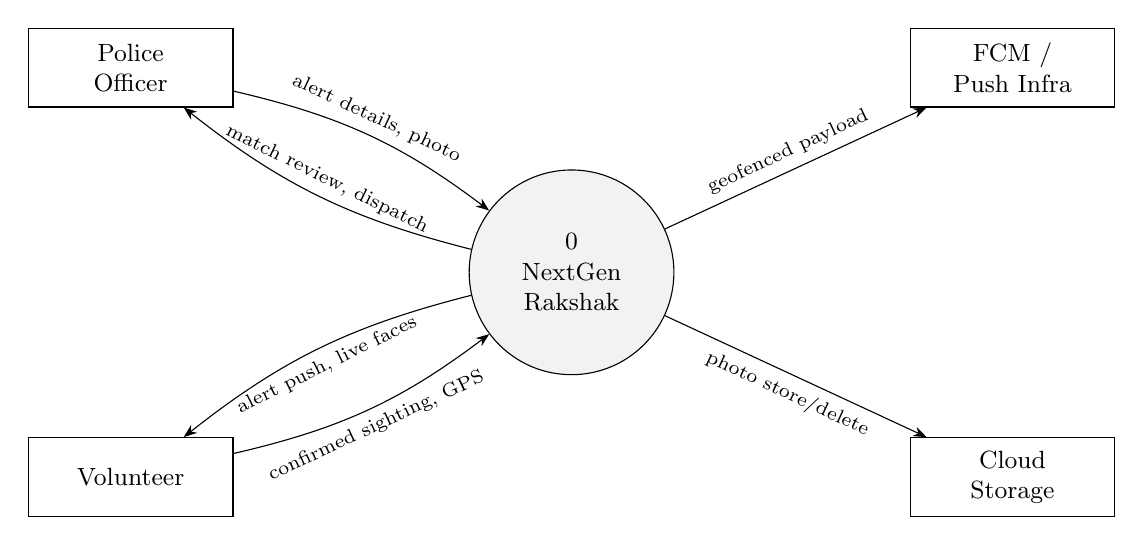
\begin{tikzpicture}[
  ext/.style={draw, minimum width=2.6cm, minimum height=1cm, align=center, font=\small},
  proc/.style={draw, circle, minimum size=2.6cm, align=center, font=\small, fill=lightgray},
  >=Stealth
]
\node[ext] (officer) at (0,2.6) {Police\\Officer};
\node[ext] (vol) at (0,-2.6) {Volunteer};
\node[proc] (p0) at (5.6,0) {0\\NextGen\\Rakshak};
\node[ext] (fcm) at (11.2,2.6) {FCM /\\Push Infra};
\node[ext] (store) at (11.2,-2.6) {Cloud\\Storage};

% each pair of opposite flows is bent apart so the two arrows -- and
% their labels -- never sit on top of one another
\draw[->] (officer) to[bend left=12]
  node[midway,above,sloped,font=\scriptsize]{alert details, photo} (p0);
\draw[->] (p0) to[bend left=12]
  node[midway,above,sloped,font=\scriptsize]{match review, dispatch} (officer);

\draw[->] (vol) to[bend right=12]
  node[midway,below,sloped,font=\scriptsize]{confirmed sighting, GPS} (p0);
\draw[->] (p0) to[bend right=12]
  node[midway,below,sloped,font=\scriptsize]{alert push, live faces} (vol);

\draw[->] (p0) -- node[midway,above,sloped,font=\scriptsize]{geofenced payload} (fcm);
\draw[->] (p0) -- node[midway,below,sloped,font=\scriptsize]{photo store/delete} (store);
\end{tikzpicture}
\caption{DFD Level 0 -- system context}
\end{figure}

\paragraph{DFD Level 1.}

\begin{figure}[H]
\centering
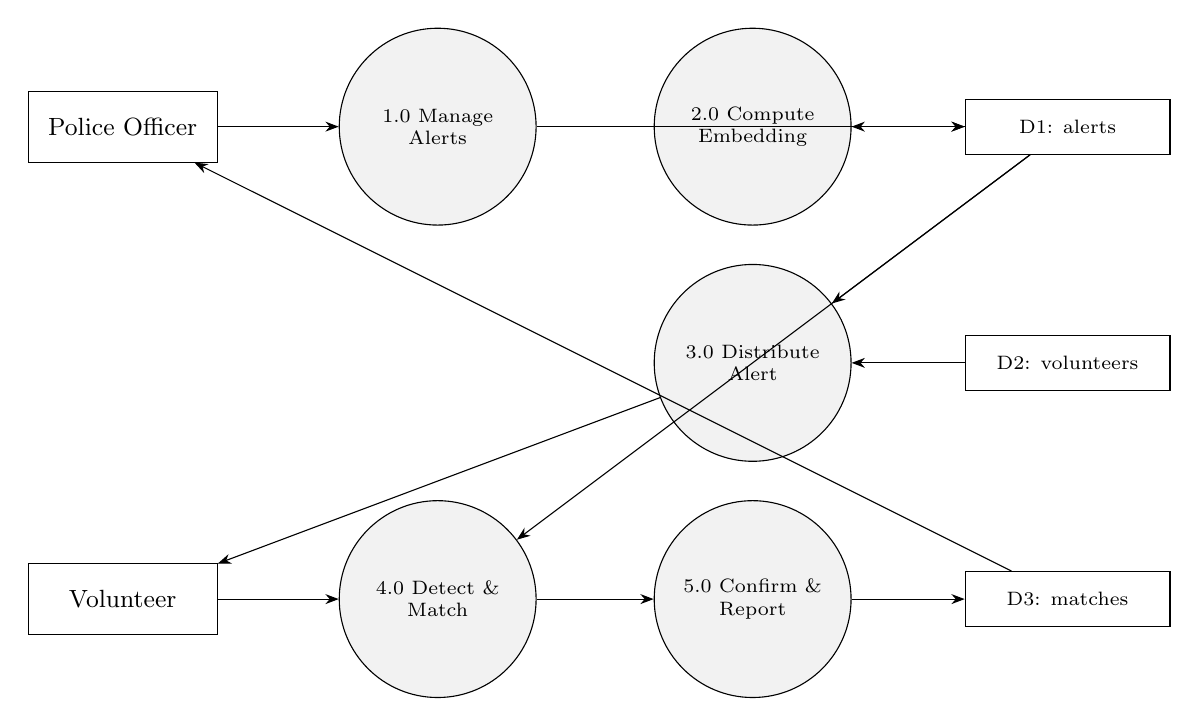
\begin{tikzpicture}[
  ext/.style={draw, minimum width=2.4cm, minimum height=0.9cm, align=center, font=\small},
  proc/.style={draw, circle, minimum size=2.5cm, align=center, font=\scriptsize, fill=lightgray},
  store/.style={draw, minimum width=2.6cm, minimum height=0.7cm, align=center, font=\scriptsize},
  >=Stealth
]
\node[ext] (officer) at (0,3) {Police Officer};
\node[ext] (vol) at (0,-3) {Volunteer};
\node[proc] (p1) at (4,3)  {1.0 Manage\\Alerts};
\node[proc] (p2) at (8,3)  {2.0 Compute\\Embedding};
\node[proc] (p3) at (8,0)  {3.0 Distribute\\Alert};
\node[proc] (p4) at (4,-3) {4.0 Detect \&\\Match};
\node[proc] (p5) at (8,-3) {5.0 Confirm \&\\Report};
\node[store] (d1) at (12,3) {D1: alerts};
\node[store] (d2) at (12,0) {D2: volunteers};
\node[store] (d3) at (12,-3) {D3: matches};

\draw[->] (officer)--(p1); \draw[->] (p1)--(d1); \draw[->] (d1)--(p2); \draw[->] (p2)--(d1);
\draw[->] (d1)--(p3); \draw[->] (d2)--(p3); \draw[->] (p3)--(vol);
\draw[->] (vol)--(p4); \draw[->] (d1)--(p4); \draw[->] (p4)--(p5); \draw[->] (p5)--(d3);
\draw[->] (d3)--(officer);
\end{tikzpicture}
\caption{DFD Level 1 -- decomposition of core processes}
\end{figure}

\subsection{Architectural Modeling}

\begin{figure}[H]
\centering
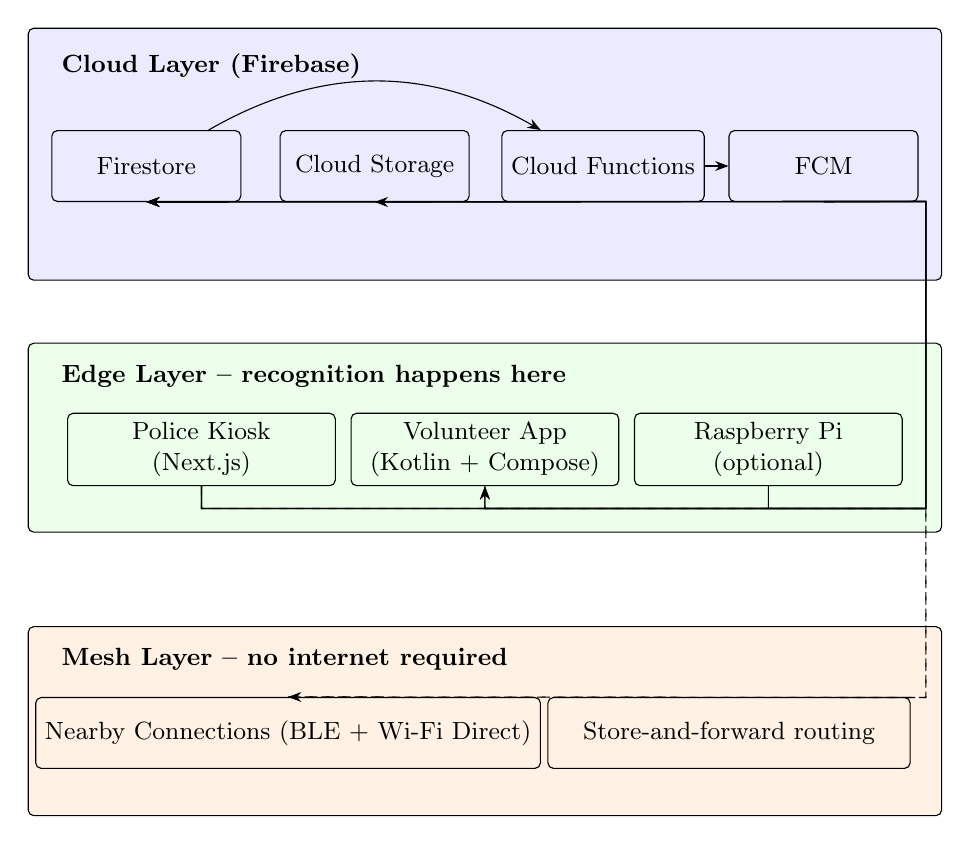
\begin{tikzpicture}[
  box/.style={draw, rounded corners=2pt, minimum height=0.9cm, align=center, font=\small},
  cloudbox/.style={box, fill=blue!8},
  edgebox/.style={box, fill=green!8},
  meshbox/.style={box, fill=orange!10},
  >=Stealth
]
% Layer titles sit INSIDE their own box, in a generous margin above the
% child boxes -- never in the inter-layer gap. Every child box's own x
% falls somewhere under at least one of these (wide) labels, so any
% arrow leaving a child box vertically is routed sideways, through a
% shared corridor at x=2.2 that sits clear of all three labels' text,
% before it ever rises or falls past a label's height band.
\node[cloudbox, minimum width=11.6cm, minimum height=3.2cm] at (0,5.2) {};
\node[font=\small\bfseries, anchor=north west] at (-5.5,6.6) {Cloud Layer (Firebase)};
\node[cloudbox, minimum width=2.4cm] (fs) at (-4.3,5.05) {Firestore};
\node[cloudbox, minimum width=2.4cm] (st) at (-1.4,5.05) {Cloud Storage};
\node[cloudbox, minimum width=2.4cm] (cf) at (1.5,5.05) {Cloud Functions};
\node[cloudbox, minimum width=2.4cm] (fcm) at (4.3,5.05) {FCM};

\node[edgebox, minimum width=11.6cm, minimum height=2.4cm] at (0,1.6) {};
\node[font=\small\bfseries, anchor=north west] at (-5.5,2.65) {Edge Layer -- recognition happens here};
\node[edgebox, minimum width=3.4cm] (kiosk) at (-3.6,1.45) {Police Kiosk\\(Next.js)};
\node[edgebox, minimum width=3.4cm] (mob) at (0,1.45) {Volunteer App\\(Kotlin + Compose)};
\node[edgebox, minimum width=3.4cm] (pi) at (3.6,1.45) {Raspberry Pi\\(optional)};

\node[meshbox, minimum width=11.6cm, minimum height=2.4cm] at (0,-2.0) {};
\node[font=\small\bfseries, anchor=north west] at (-5.5,-0.95) {Mesh Layer -- no internet required};
\node[meshbox, minimum width=5.4cm] (nc) at (-2.5,-2.15) {Nearby Connections (BLE + Wi-Fi Direct)};
\node[meshbox, minimum width=4.6cm] (rt) at (3.1,-2.15) {Store-and-forward routing};

% -- Cloud-layer internal flow: Firestore -> Cloud Functions arcs OVER
%    Cloud Storage instead of cutting through it; the rest are adjacent.
\draw[->] (fs) to[bend left=30] (cf);
\draw[->] (cf) -- (fcm);

% -- Cross-layer wiring. Every row has an empty margin below its child
%    boxes (nothing lives there -- the title label sits in the margin
%    ABOVE instead). Every connector: drops out of its source box into
%    that empty lower margin, travels sideways there (safe at any x,
%    since the margin is empty) out to a shared vertical corridor at
%    x=5.6 that clears every box in every row, rides that corridor past
%    whichever layer(s) it needs to cross, then travels sideways again
%    in the TARGET row's own lower margin before a short final rise
%    directly into the target from below. No segment ever needs to
%    pass over another child box or through a label.
\draw[->] (kiosk.south) -- (-3.6,0.7) -- (5.6,0.7) -- (5.6,4.6) -- (fs.south);
\draw[->] (kiosk.south) -- (-3.6,0.7) -- (5.6,0.7) -- (5.6,4.6) -- (st.south);
\draw[->] (mob.south)   -- (0,0.7)    -- (5.6,0.7) -- (5.6,4.6) -- (fs.south);
\draw[->] (pi.south)    -- (3.6,0.7)  -- (5.6,0.7) -- (5.6,4.6) -- (fs.south);
\draw[->] (fcm.south)   -- (5.6,4.6)  -- (5.6,0.7) -- (0,0.7)   -- (mob.south);

\draw[->, dashed] (kiosk.south) -- (-3.6,0.7) -- (5.6,0.7) -- (5.6,-1.7) -- (nc.north);
\draw[->, dashed] (nc.north)    -- (5.6,-1.7) -- (5.6,0.7) -- (0,0.7)    -- (mob.south);
\end{tikzpicture}
\caption{Three-layer system architecture: Cloud, Edge, Mesh}
\label{fig:arch}
\end{figure}

\begin{figure}[H]
\centering
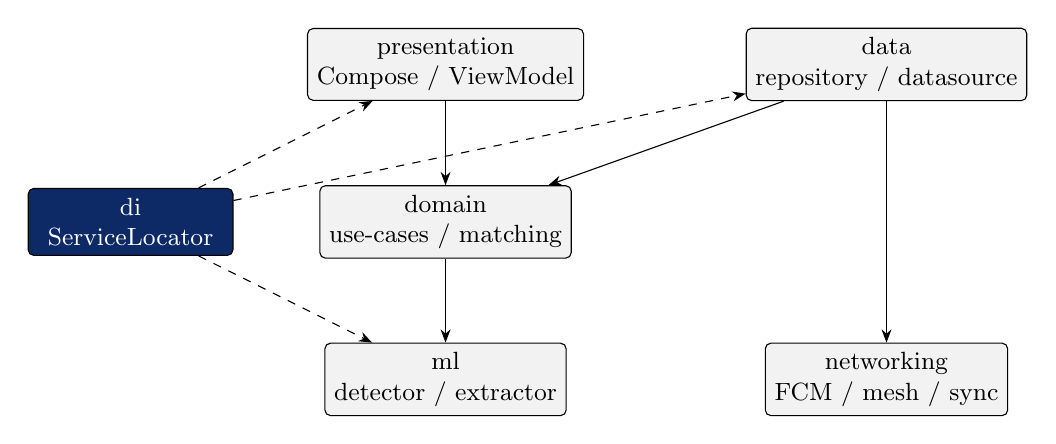
\begin{tikzpicture}[
  box/.style={draw, rounded corners=2pt, minimum height=0.85cm, minimum width=2.6cm, align=center, font=\small, fill=lightgray},
  >=Stealth
]
\node[box] (p) at (0,2) {presentation\\Compose / ViewModel};
\node[box] (d) at (0,0) {domain\\use-cases / matching};
\node[box] (da) at (5.6,2) {data\\repository / datasource};
\node[box] (n) at (5.6,-2) {networking\\FCM / mesh / sync};
\node[box] (ml) at (0,-2) {ml\\detector / extractor};
\node[box, fill=rakshaknavy, text=white] (di) at (-4.0,0) {di\\ServiceLocator};

\draw[->] (p) -- (d); \draw[->] (da) -- (d); \draw[->] (da) -- (n); \draw[->] (d) -- (ml);
\draw[dashed,->] (di) -- (p); \draw[dashed,->] (di) -- (da); \draw[dashed,->] (di) -- (ml);
\end{tikzpicture}
\caption{Volunteer Android app -- layered (SOLID) package architecture}
\end{figure}

\section{Mathematical Modeling}

The system is formally represented as:
\[
S = \{ I,\ P,\ O,\ F_{\text{main}},\ D_D,\ D_{\text{fail}} \}
\]
where
\begin{align*}
I &= \{\text{alert photo}, \text{case details}, \text{live camera frames}, \text{GPS fix}\} && \text{(inputs)}\\
P &= \{\text{detect}, \text{align}, \text{embed}, \text{compare}, \text{confirm}, \text{route}, \text{dispatch}\} && \text{(processes)}\\
O &= \{\text{confirmed sighting}, \text{dispatch decision}\} && \text{(outputs)}\\
D_D &= \text{successfully reported, GPS-tagged, officer-reviewed sighting} && \text{(success)}\\
D_{\text{fail}} &= \{\text{no camera / no GPS / low light / occluded face}\} && \text{(failure)}
\end{align*}

Face matching itself is a function
\[
\mathrm{match}(e_1, e_2) =
\begin{cases}
1 & \text{if } \cos\theta = \dfrac{e_1 \cdot e_2}{\lVert e_1\rVert \lVert e_2\rVert} > \tau \\[4pt]
0 & \text{otherwise}
\end{cases}
\]
where $e_1, e_2 \in \mathbb{R}^{128}$ are L2-normalised face embeddings and
$\tau = 0.55$ is the measured decision threshold (\S\ref{sec:threshold-measurement}). Because both
$e_1$ and $e_2$ are unit vectors, cosine similarity reduces to their dot
product, making the comparison a single, cheap floating-point operation
suitable for repeated per-frame execution on a mobile CPU.

\subsection{Venn Diagram}

Figure~\ref{fig:venn} formalises the research gap already identified
qualitatively in Table~\ref{tab:litreview}: every reviewed existing system
falls inside at least one of three structural-limitation sets --
\emph{Centralised}, \emph{Internet-dependent}, and \emph{Reactive} --
whereas NextGen Rakshak is positioned outside all three.

\begin{figure}[H]
\centering
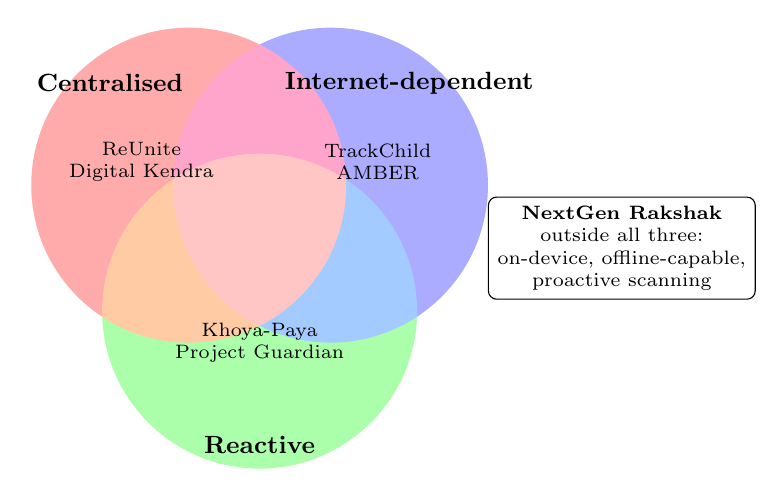
\begin{tikzpicture}
\begin{scope}[blend group = soft light, opacity=0.55]
\fill[red!60]    ( -0.9,0.6) circle (2.0);
\fill[blue!60]   ( 0.9,0.6)  circle (2.0);
\fill[green!60]  ( 0,-1.0)   circle (2.0);
\end{scope}
\node at (-1.9,1.9) {\small\bfseries Centralised};
\node at (1.9,1.9)  {\small\bfseries Internet-dependent};
\node at (0,-2.7)   {\small\bfseries Reactive};
\node[align=center, font=\scriptsize] at (-1.5,0.9) {ReUnite\\Digital Kendra};
\node[align=center, font=\scriptsize] at (1.5,0.9) {TrackChild\\AMBER};
\node[align=center, font=\scriptsize] at (0,-1.4) {Khoya-Paya\\Project Guardian};
\node[draw, rounded corners=3pt, fill=white, align=center, font=\scriptsize] at (4.6,-0.2)
  {\textbf{NextGen Rakshak}\\outside all three:\\on-device, offline-capable,\\proactive scanning};
\end{tikzpicture}
\caption{Venn diagram -- structural limitations of existing systems vs.\ NextGen Rakshak's position}
\label{fig:venn}
\end{figure}

% ============================================================================
%  CHAPTER 5 -- RISK MANAGEMENT
% ============================================================================
\chapter{Risk Management}

\section{Risk Identification}

Ten risks were identified and tracked across the project, ranked by
expected damage to the project rather than by probability alone.

\begin{longtable}{|p{1.0cm}|p{5.3cm}|p{2.1cm}|p{4.7cm}|}
\caption{Risk register}
\label{tab:risk}\\
\hline
\textbf{ID} & \textbf{Risk} & \textbf{Impact} & \textbf{Owner} \\
\hline
\endfirsthead
\hline
\textbf{ID} & \textbf{Risk} & \textbf{Impact} & \textbf{Owner} \\
\hline
\endhead
R1  & Server-side ML runtime (\code{tfjs-node}) fails to load in the deployed Cloud Functions environment & Critical & Cloud/Functions owner \\ \hline
R2  & No suitable, ethically sourced children's face dataset for recognition-accuracy validation & High & ML/evaluation owner \\ \hline
R3  & The offline mesh has never been validated across real, physically separate devices & High & Mesh owner \\ \hline
R4  & Final-report writing load exceeds what one person can produce in the time remaining & High & Report lead \\ \hline
R5  & Feature freeze slips and features are still being added during report-writing weeks & High & Project lead \\ \hline
R6  & Live demo fails on stage due to venue Wi-Fi, FCM latency, or device issues & High & All members \\ \hline
R7  & Low automated test coverage leaves most code paths unverified by anything but manual testing & Medium & QA owner \\ \hline
R8  & No officer is authorised, so the kiosk cannot be used by anyone until this is fixed & Medium & Auth owner \\ \hline
R9  & The offline demo path cannot render the child's photo without internet, since only a URL is carried by default & Medium & Mesh/UI owner \\ \hline
R10 & Four people committing directly to \code{main} produces avoidable merge conflicts & Low--Medium & Project lead \\
\hline
\end{longtable}

\section{Strategies Used to Manage Risk}

\begin{table}[H]
\centering
\caption{Mitigation strategy per identified risk}
\begin{tabular}{|p{0.8cm}|p{11.2cm}|}
\hline
\textbf{ID} & \textbf{Mitigation} \\
\hline
R1 & Deploy early rather than late, so a runtime failure is caught with time to react; fallback plan was to compute the embedding client-side with TensorFlow.js at alert creation instead of server-side. \\ \hline
R2 & Ordered fallback: seek a licensed academic dataset first; else use team members' own consented childhood photographs; failing both, report the adult-only measurement plainly as an upper-bound proxy rather than a child-accuracy result, and list it as Future Scope. \\ \hline
R3 & Budget a full day for a dedicated multi-device trial with verbose logging added \emph{before} the trial, not after; report the maximum hop count actually observed rather than an unverified claim. \\ \hline
R4 & Confirm early whether a conference paper is required (removes significant load if not); start results-chapter writing the moment the last measurement is available, not after. \\ \hline
R5 & Enforce a hard feature-freeze date; anything unfinished at that point becomes a documented Future Scope item, not a late addition. \\ \hline
R6 & Prepare a pre-recorded demo video, a personal-hotspot network backup, and printed screenshots; lead with the offline-mesh demo, since it is the scenario that needs no network at all. \\ \hline
R7 & Raise unit-test coverage on the core matching/mesh logic and exercise every functional requirement at least once before submission. \\ \hline
R8 & Fix officer self-registration (the \code{claimOfficerRole} function) early and verify both the grant path and the deny path explicitly. \\ \hline
R9 & Carry a small, highly compressed JPEG thumbnail of the child's face inside the mesh packet itself, so the offline confirmation dialog can render a photo with zero internet. \\ \hline
R10 & Adopt short-lived feature branches and pull requests once parallel development begins, rather than direct commits to \code{main}. \\
\hline
\end{tabular}
\end{table}

\section{Risk Projection}

\subsection{Preparing Risk Table}

Risks were re-scored qualitatively (Low / Medium / High) on probability and
impact, and a priority derived from their product, to decide where limited
remaining project time should go.

\begin{table}[H]
\centering
\caption{Risk projection -- probability $\times$ impact}
\begin{tabular}{|p{0.8cm}|p{4.4cm}|p{2.0cm}|p{2.0cm}|p{2.4cm}|}
\hline
\textbf{ID} & \textbf{Risk} & \textbf{Probability} & \textbf{Impact} & \textbf{Priority} \\
\hline
R1 & \code{tfjs-node} runtime failure & Medium & Critical & \textbf{Highest} \\ \hline
R3 & Mesh unverified on real devices & Medium & High & \textbf{High} \\ \hline
R2 & No children's face dataset & High & High & \textbf{High} \\ \hline
R6 & Live demo failure & Medium & High & \textbf{High} \\ \hline
R5 & Feature-freeze slip & Medium--High & High & \textbf{High} \\ \hline
R4 & Report-writing overload & Medium--High & High & Medium--High \\ \hline
R8 & No authorised officer & Certain (until fixed) & Medium & Medium \\ \hline
R9 & Offline demo shows no photo & High (without fix) & Medium & Medium \\ \hline
R7 & Low test coverage & Certain & Medium & Medium \\ \hline
R10 & No branch discipline & Medium & Low--Medium & Low \\
\hline
\end{tabular}
\end{table}

\section{Feasibility}

\subsection*{Technical feasibility}
Every component relies on mature, freely available, and well-documented
technology: Google ML Kit \cite{mlkit} and TensorFlow Lite \cite{tflite}
ship with pretrained, production-grade models; Firebase \cite{firebase}
provides a realtime backend with no server for the team to operate; and
Nearby Connections \cite{nearby} is a maintained Google Play Services API
rather than a custom radio protocol. The riskiest
technical assumption -- that a lightweight, on-device model could achieve
useful discrimination -- was validated directly through the threshold
measurement in \S\ref{sec:threshold-measurement}, rather than assumed. The project is therefore judged
technically feasible for a four-member student team within one academic
year.

\subsection*{Operational feasibility}
The volunteer model targets pre-registered, duty-bound participants
(police, NCC/NSS cadets, NGO staff, shopkeepers) already present at mass
gatherings in an official or semi-official capacity, rather than requiring
spontaneous adoption by the general public -- this matches how Indian
festival security is actually staffed today, and keeps onboarding to a
single Google sign-in.

\subsection*{Economic feasibility}
The entire stack sits within free or near-free tiers for a project of this
scale: Firebase's Spark/Blaze free-tier quotas comfortably cover a
demonstration deployment; ML Kit, TensorFlow Lite, and Nearby Connections
carry no licensing cost; and hardware requirements are ordinary
Android phones the volunteer network already owns. The only new hardware
is the optional Raspberry Pi node, budgeted at under 5{,}000 (Table 2.5.1)
and explicitly scoped as optional.

\subsection*{Schedule feasibility}
The twelve-phase schedule (Table~\ref{tab:schedule}) allocates dedicated
weeks to integration and stress testing (Phase 6), performance tuning
(Phase 8), and a field demonstration (Phase 10) before report and paper
deadlines, rather than compressing verification into the final days --
directly addressing the schedule risks (R4, R5) identified in \S5.1.

% ============================================================================
%  CHAPTER 6 -- TECHNICAL SPECIFICATION
% ============================================================================
\chapter{Technical Specification}

\section{Software requirement specification}

\subsection{Operating System (OS)}
Development was carried out across Windows, Linux, and macOS workstations
(the toolchain -- Node.js, Android Studio/Gradle, Python -- is
cross-platform). The volunteer application targets Android \code{minSdk 24}
(Android 7.0) through \code{compileSdk 35} (Android 15); the kiosk portal
runs in any modern evergreen browser (Chrome, Edge, Firefox) on the police
booth's existing device, requiring no dedicated OS.

\subsection{Integrated Development Environment (IDE)}
\begin{itemize}
  \item \textbf{Android Studio} -- volunteer app development, Gradle
        builds, on-device debugging and the LayoutInspector for the
        Compose UI.
  \item \textbf{Visual Studio Code} -- Next.js/TypeScript kiosk portal and
        Cloud Functions development.
  \item \textbf{Figma} -- UI/UX wireframing for both the kiosk and mobile
        screens.
  \item \textbf{Postman} -- manual exercising of Cloud Function callable
        endpoints during development.
\end{itemize}

\subsection{Programming Language and Database}

\begin{table}[H]
\centering
\caption{Languages, frameworks, and data store by component}
\begin{tabular}{|p{3.6cm}|p{9.9cm}|}
\hline
\textbf{Component} & \textbf{Language / Framework} \\
\hline
Police kiosk portal & TypeScript, Next.js 14 (App Router), React 18, Tailwind CSS, shadcn/ui \\ \hline
Volunteer Android app & Kotlin, Jetpack Compose, Coroutines, Room (SQLite), DataStore \\ \hline
Cloud Functions & TypeScript, Node.js 22, \code{firebase-functions} v7, \code{@tensorflow/tfjs-node} \\ \hline
Model tooling & Python 3.10--3.12, TensorFlow, ONNX \\ \hline
Database & Cloud Firestore (NoSQL document store) -- collections \code{alerts}, \code{matches}, \code{officers}, \code{volunteers}; on-device Room (SQLite) for the offline match/mesh queue \\
\hline
\end{tabular}
\end{table}

\section{Hardware Requirement Specifications}

\begin{table}[H]
\centering
\caption{Minimum and recommended hardware}
\begin{tabular}{|p{3.6cm}|p{4.6cm}|p{4.6cm}|}
\hline
\textbf{Device} & \textbf{Minimum} & \textbf{Recommended} \\
\hline
Volunteer phone & Android 7.0 (API 24), 2\,GB RAM, rear camera, Bluetooth LE & Android 10+, 4\,GB RAM, dual-SIM, GPS \\ \hline
Kiosk device & Any laptop/tablet with a modern browser & Laptop with a stable network connection \\ \hline
Development machine & 8\,GB RAM, JDK 17, Node.js 18+ & 16\,GB RAM, SSD, Node.js 22 \\ \hline
Raspberry Pi node (optional) & Pi 4 (4\,GB) + Camera Module V2 & Pi 4 (4\,GB) + Camera Module V2 + active cooling \\
\hline
\end{tabular}
\end{table}

% ============================================================================
%  CHAPTER 7 -- IMPLEMENTATION DETAILS
% ============================================================================
\chapter{Implementation Details}

This chapter documents how each module described in \S3.3 and \S4.5 was
actually implemented, with representative code and screenshots of the
working system.

\section{Firestore Data Model}
\label{sec:firestore-schema}

Every component reads and writes the same four Firestore collections. The
schema is deliberately \emph{denormalised} -- a \code{matches} document
copies \code{childName} and \code{imageUrl} from its parent alert -- so
that the kiosk's live feed and the volunteer's match history each render
from a single collection listener, with no join and no second round-trip.

\begin{table}[H]
\centering
\caption{\code{alerts/\{alertId\}} -- the missing-child case record}
\begin{tabular}{|p{3.4cm}|p{2.2cm}|p{7.1cm}|}
\hline
\textbf{Field} & \textbf{Type} & \textbf{Notes} \\
\hline
\code{childName}, \code{age}, \code{gender} & string, number, string & Displayed on every volunteer device \\ \hline
\code{clothingDesc}, \code{identifyingMarks} & string & Human search aid; usable even if recognition fails \\ \hline
\code{parentContact} & string & Kiosk-only; never sent to volunteer devices or the mesh \\ \hline
\code{imageUrl} & string & Cloud Storage URL; blanked when the case resolves \\ \hline
\code{embedding} & number[] & 128-d fallback vector; written by \code{onAlertCreated}; cleared on resolve \\ \hline
\code{lastSeen}, \code{lastSeenDate/Time} & string & Free-text place plus a structured date/time \\ \hline
\code{geoLocation} & GeoPoint? & Kiosk's fix at filing; drives the 2\,km geofence \\ \hline
\code{status} & string & \code{active} $\mid$ \code{resolved} \\ \hline
\code{timestamp} & Timestamp & Server clock; drives expiry and elapsed-time display \\
\hline
\end{tabular}
\end{table}

\begin{table}[H]
\centering
\caption{\code{matches/\{matchId\}} -- a volunteer-confirmed sighting}
\begin{tabular}{|p{3.4cm}|p{2.2cm}|p{7.1cm}|}
\hline
\textbf{Field} & \textbf{Type} & \textbf{Notes} \\
\hline
\code{alertId} & string & Rules require the referenced alert to exist \\ \hline
\code{childName}, \code{imageUrl} & string & Denormalised for single-listener rendering \\ \hline
\code{volunteerId}, \code{volunteerName} & string & Reporter's Auth uid and display name \\ \hline
\code{relayedBy} & string? & Set only when a \emph{different} device uploaded it off the mesh \\ \hline
\code{location}, \code{hasLocation} & GeoPoint, bool & \code{hasLocation=false} suppresses the map pin instead of drawing $(0,0)$ \\ \hline
\code{confidence} & number & Cosine score, clamped to $[0,1]$ \\ \hline
\code{status} & string & \code{pending} $\mid$ \code{dispatched} $\mid$ \code{accepted} $\mid$ \code{dismissed} -- only the kiosk may change it \\ \hline
\code{timestamp} & Timestamp & Must equal \code{request.time}; no back-dating \\
\hline
\end{tabular}
\end{table}

\code{officers/\{uid\}} (kiosk directory) holds
\code{uid, email, photoURL, role, displayName, phone, station, badgeNumber,
fcmToken?, createdAt, lastLoginAt, updatedAt} and is written once by
\code{claimOfficerRole} (Listing~7.1); the browser may only patch
\code{displayName/phone/station/badgeNumber/fcmToken}. \code{volunteers/\{uid\}}
(mobile directory) holds \code{phone, role, name, email, photoUrl, fcmToken,
registeredAt, lastLocation, locationUpdatedAt} and is written by its own
device only. One composite index, \code{alerts(status ASC, timestamp DESC)},
covers both the kiosk dashboard and the volunteer home screen's active-alert
query.

\section{Police Kiosk Portal}

Built with Next.js 14 (App Router), the kiosk exposes five guarded routes --
\code{/login}, \code{/} (dashboard), \code{/alerts/new}, \code{/alerts/history},
\code{/matches}, and \code{/profile} -- behind a shell that blocks all
protected content until the signed-in account's \code{police} custom claim
has been confirmed, so no officer-only data ever flashes on screen for an
unauthorised viewer.

\begin{figure}[H]
\centering
\begin{subfigure}[t]{0.48\textwidth}
  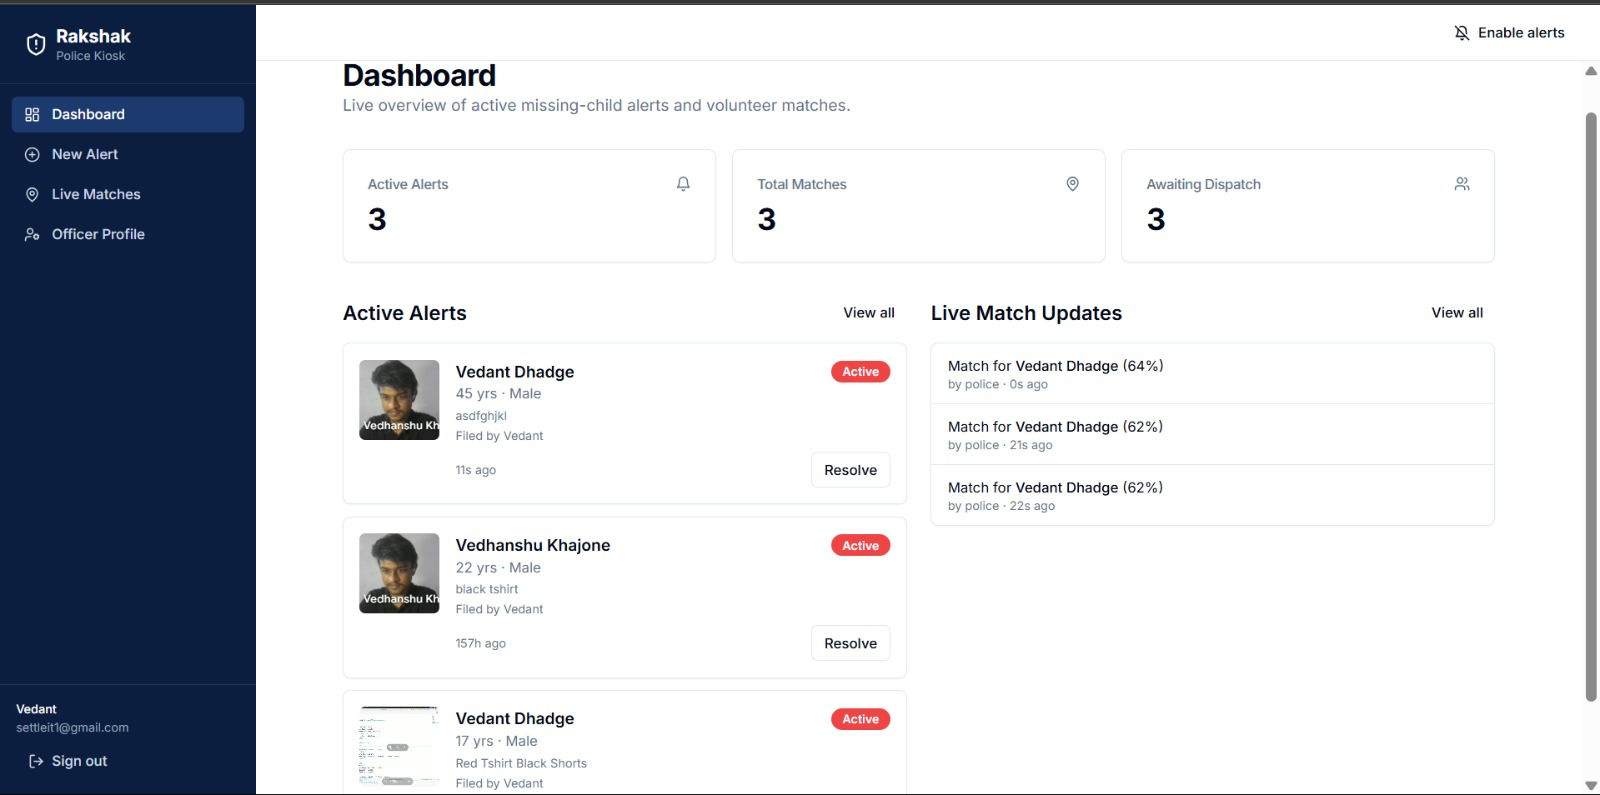
\includegraphics[width=\linewidth]{images/ss_web_dashboard.jpg}
  \caption{Live dashboard: stat tiles, active alerts, match feed}
\end{subfigure}\hfill
\begin{subfigure}[t]{0.48\textwidth}
  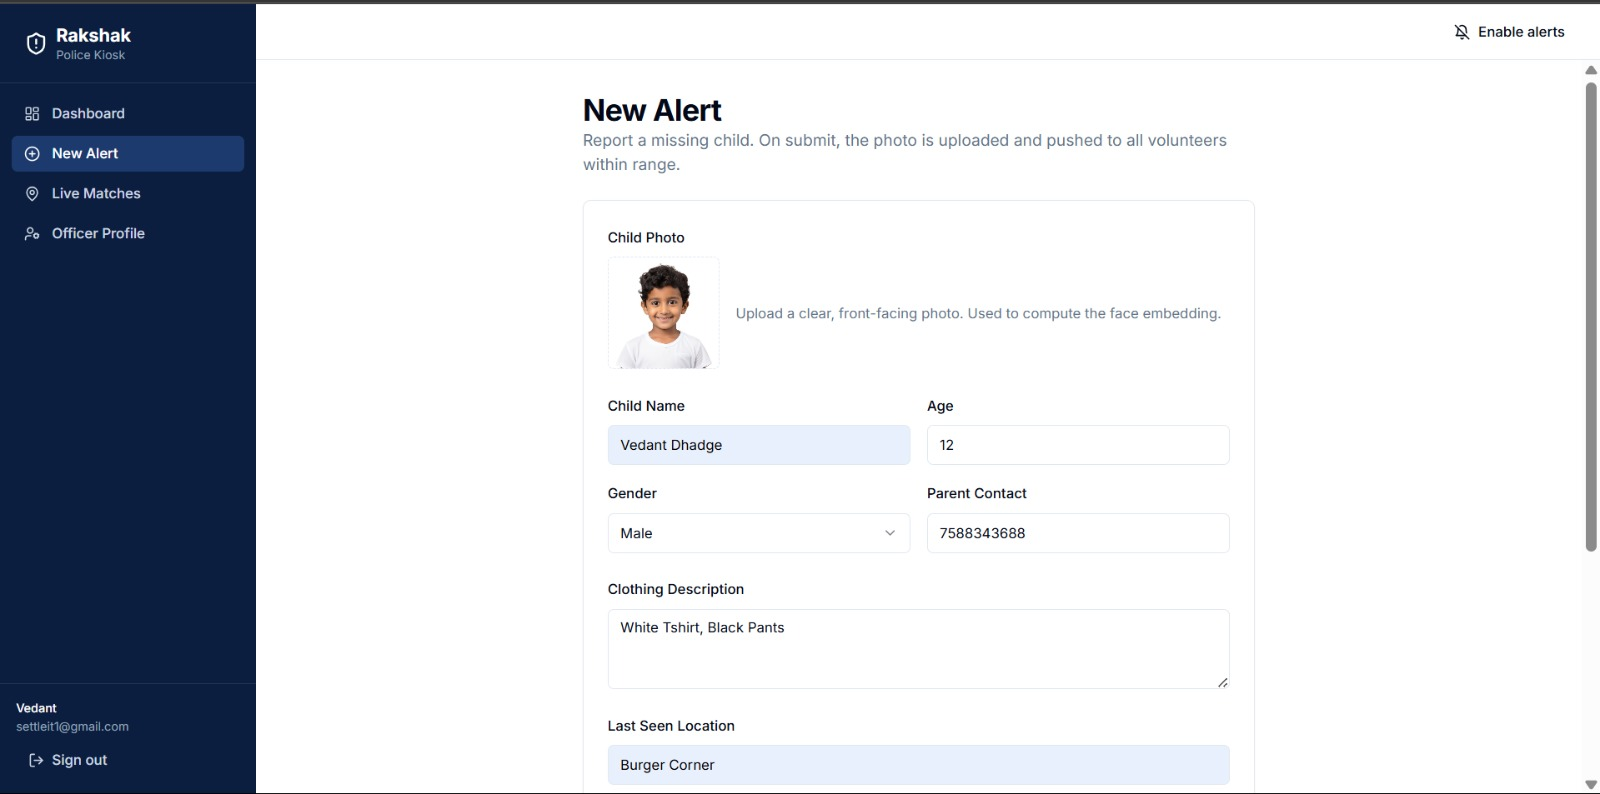
\includegraphics[width=\linewidth]{images/ss_web_new_alert.jpg}
  \caption{New Alert form -- photo, details, geolocation}
\end{subfigure}
\caption{Police kiosk portal}
\end{figure}

\subsection*{Authentication and authorisation}
Both the kiosk and the mobile app share a single Firebase Authentication
pool, but authentication (proving who you are) is deliberately kept
separate from authorisation (what you may do). Signing in with Google
proves identity only; the ability to create an alert is gated on a
\code{police} custom claim, granted by the \code{claimOfficerRole} callable
Cloud Function.

\begin{lstlisting}[language=TypeScript, caption={Officer self-registration -- excerpt of \texttt{functions/src/officers.ts}}]
export const claimOfficerRole = onCall(async (request) => {
  const uid = requireAuth(request);
  const volunteerDoc = await db.doc(`volunteers/${uid}`).get();

  if (volunteerDoc.exists) {
    // One account, one role: refuse and revoke any stale claim.
    await auth.setCustomUserClaims(uid, { police: false });
    await auth.revokeRefreshTokens(uid);
    throw new HttpsError("permission-denied",
      "This account is already registered as a volunteer.");
  }

  await auth.setCustomUserClaims(uid, { police: true });
  await db.doc(`officers/${uid}`).set({
    uid, role: "police", createdAt: FieldValue.serverTimestamp(),
    lastLoginAt: FieldValue.serverTimestamp(),
  }, { merge: true });
});
\end{lstlisting}

\subsection{Alert Creation and the Kiosk Data API}
\label{sec:kiosk-data-api}

All Firestore access on the web side is funnelled through two thin
modules -- \code{lib/firestore.ts} and \code{lib/officers.ts} -- rather
than scattering \code{onSnapshot}/\code{addDoc} calls through components.
This keeps the security-relevant write shape (which fields a client is
allowed to send) in one place, one call site per operation:

\begin{table}[H]
\centering
\caption{Kiosk data API surface (\texttt{lib/firestore.ts}, \texttt{lib/officers.ts})}
\begin{tabular}{|p{4.4cm}|p{8.1cm}|}
\hline
\textbf{Function} & \textbf{Does} \\
\hline
\code{uploadChildPhoto} & Sanitises the filename, uploads to \code{alert\_images/}, returns the download URL \\ \hline
\code{createAlert} & Writes the \code{alerts} document; captures \code{navigator.geolocation} if the browser permits it \\ \hline
\code{resolveAlert} & Flips \code{status} to \code{resolved}, triggering \code{onAlertResolved} (\S\ref{sec:privacy-purge}) \\ \hline
\code{subscribeActiveAlerts}, \code{subscribeAllAlerts} & Live \code{onSnapshot} listeners behind the dashboard and history page \\ \hline
\code{subscribeMatches}, \code{fetchMatchCounts} & Live 100-doc match feed, plus five parallel \code{getCountFromServer} aggregates for exact dashboard tile counts \\ \hline
\code{acceptMatch}, \code{dismissMatch}, \code{dispatchMatch} & Kiosk-only status transitions on a \code{matches} document \\ \hline
\code{subscribeOfficer}, \code{updateOfficerProfile}, \code{saveOfficerFcmToken} & Officer directory read/write, restricted to the whitelisted profile fields \\
\hline
\end{tabular}
\end{table}

The alert-creation form requires a photo, name, age, gender, clothing
description, contact number, and last-seen place/date/time; \code{identifyingMarks}
is optional. The upload filename is sanitised with \code{safeFileName}
before it reaches Storage, because the \code{alert\_images/\{imageId\}}
rule matches a single path segment -- an unescaped slash in a filename
would silently step outside the intended rule.

\subsection{Match Review and Dispatch}

The \code{/matches} route renders each pending sighting beside the original
alert photo, so the officer never has to context-switch to judge a match.
A reviewed match locks: once \code{accept}, \code{dismiss}, or
\code{dispatch} has been called, the dialog cannot be reopened for that
document.

\begin{lstlisting}[language=TypeScript, caption={Match status transition -- excerpt of \texttt{lib/firestore.ts}}]
export async function dispatchMatch(matchId: string) {
  await updateDoc(doc(db, "matches", matchId), {
    status: "dispatched",
  });
  // A Google Maps deep link is built client-side from the match's own
  // GeoPoint -- no extra write, no extra round-trip.
}

export async function dismissMatch(matchId: string) {
  await updateDoc(doc(db, "matches", matchId), { status: "dismissed" });
}
\end{lstlisting}

The review dialog additionally: flags a sighting relayed off the mesh
(\code{relayedBy} set) so the officer knows the reporting volunteer was
offline; suppresses the map link entirely when \code{hasLocation} is
\code{false}, rather than plotting a misleading pin at $(0,0)$; and shows
the volunteer's self-reported role (police/NCC/NGO/community) so the
officer can weigh a sighting's credibility at a glance.

\section{Volunteer Android Application}

The application follows a clean, SOLID-aligned package layout
(\code{data} / \code{domain} / \code{ml} / \code{networking} /
\code{presentation}) wired together with a hand-written
\code{ServiceLocator}, keeping dependency wiring in one place without the
build-time cost of a DI framework on a student project.

\begin{figure}[H]
\centering
\begin{subfigure}[t]{0.31\textwidth}
  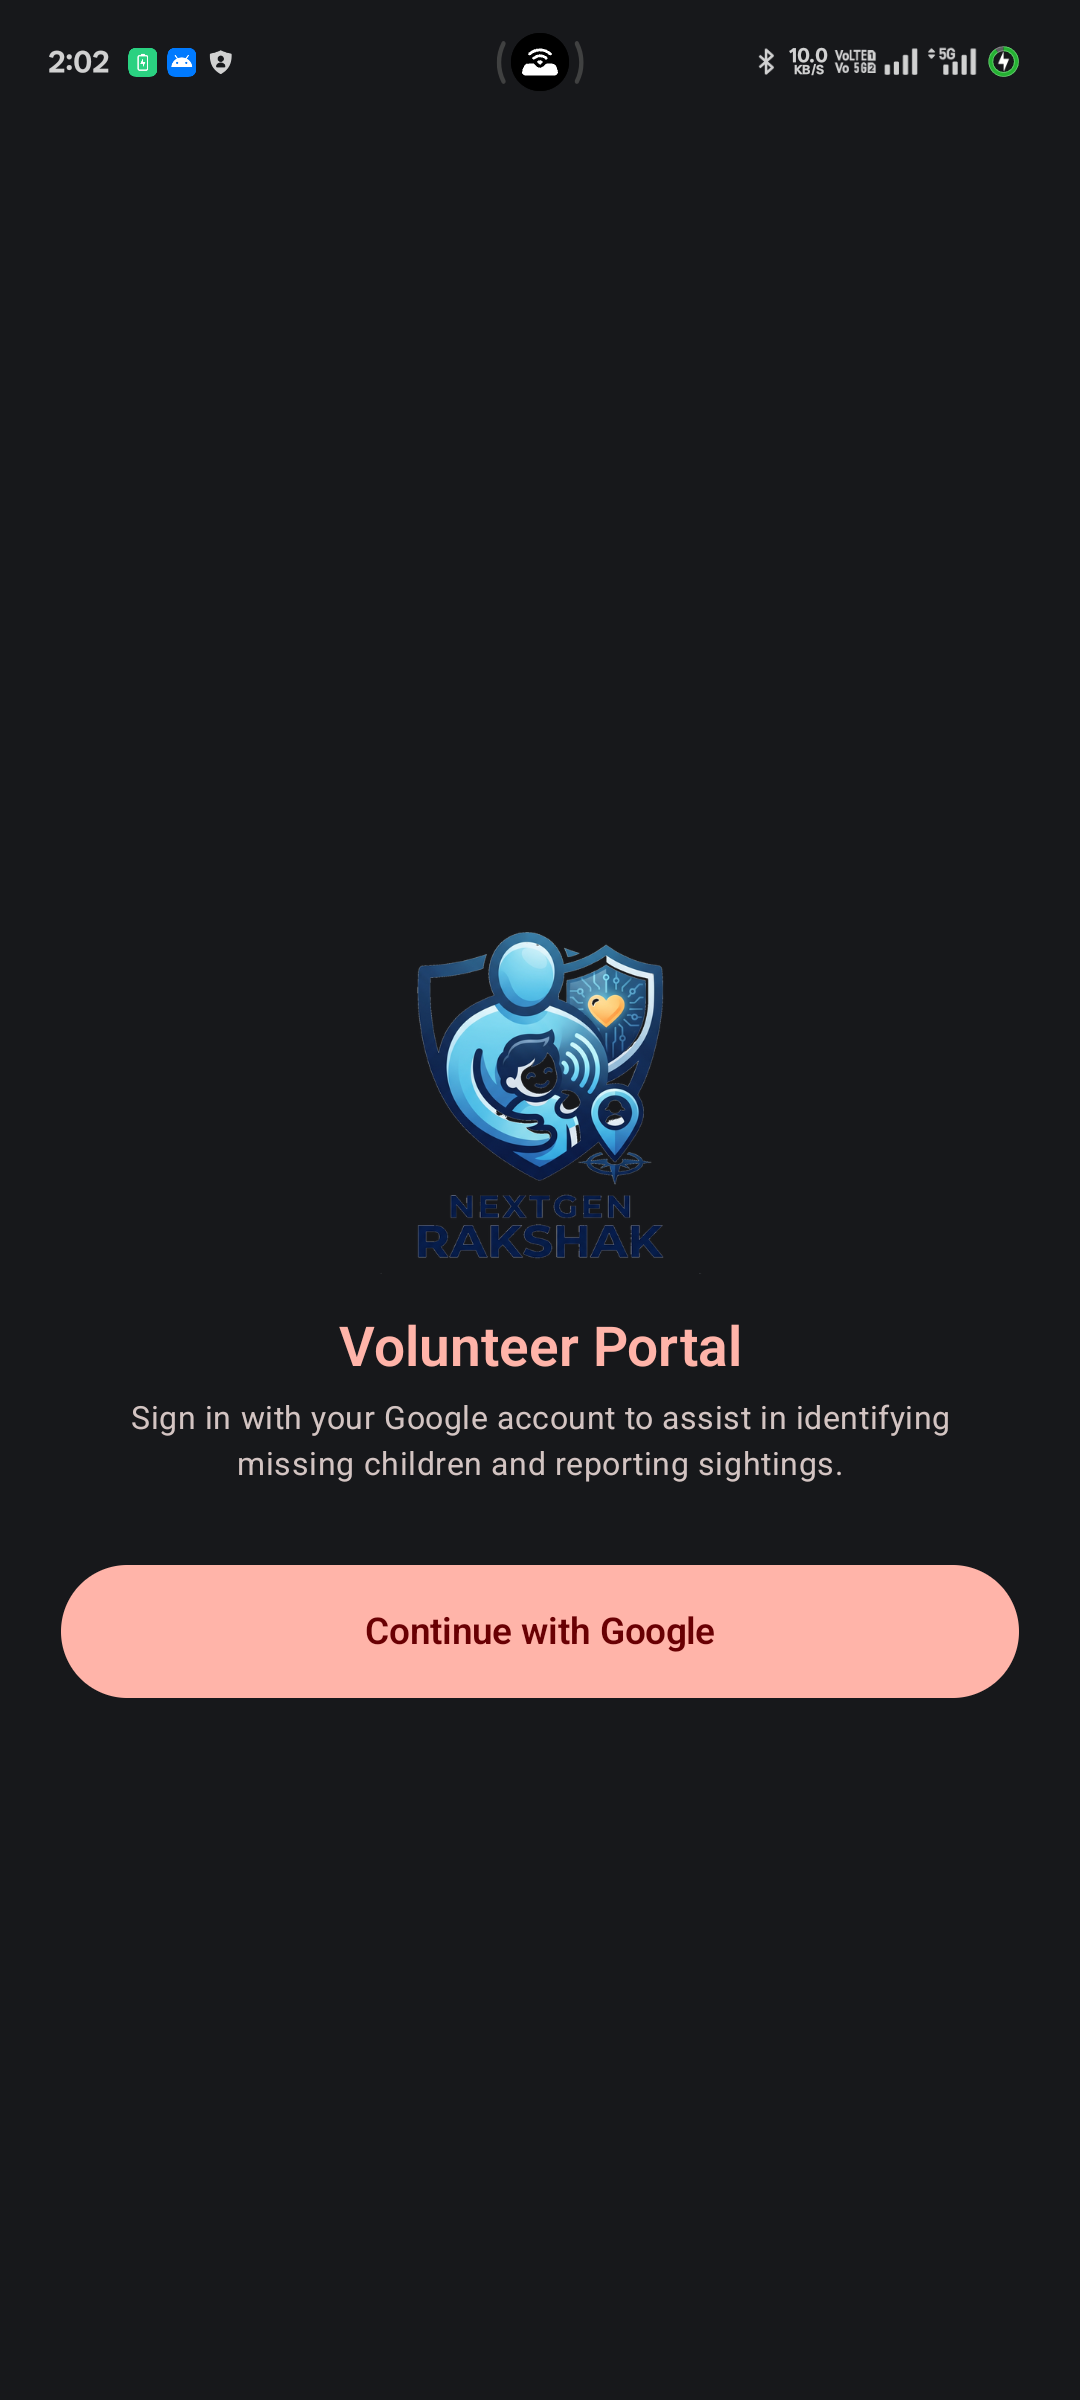
\includegraphics[width=\linewidth]{images/ss_01_login.png}
  \caption{Login}
\end{subfigure}\hfill
\begin{subfigure}[t]{0.31\textwidth}
  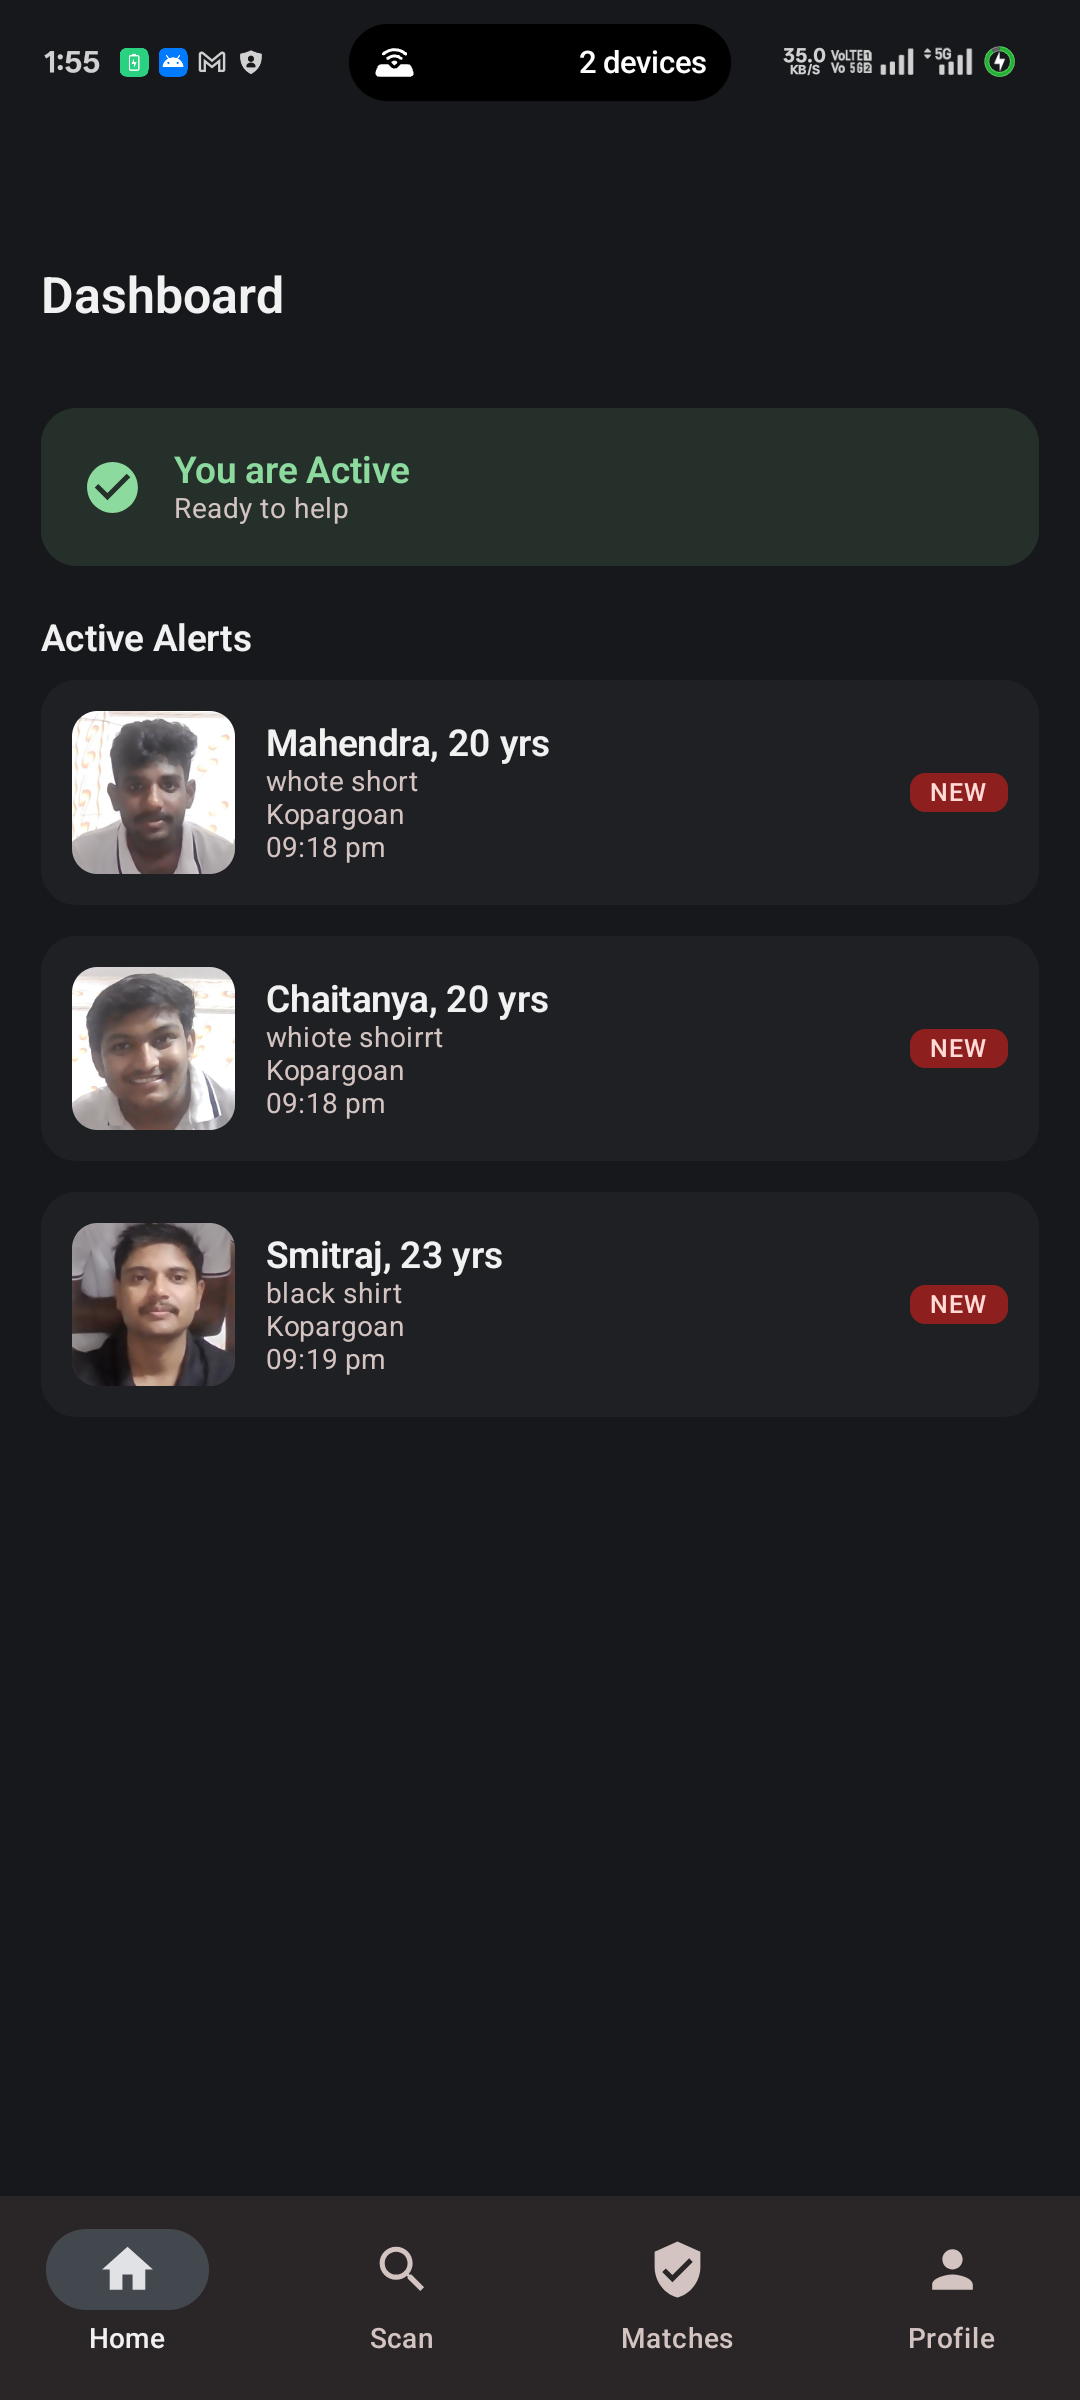
\includegraphics[width=\linewidth]{images/ss_04_home.png}
  \caption{Home -- active alerts}
\end{subfigure}\hfill
\begin{subfigure}[t]{0.31\textwidth}
  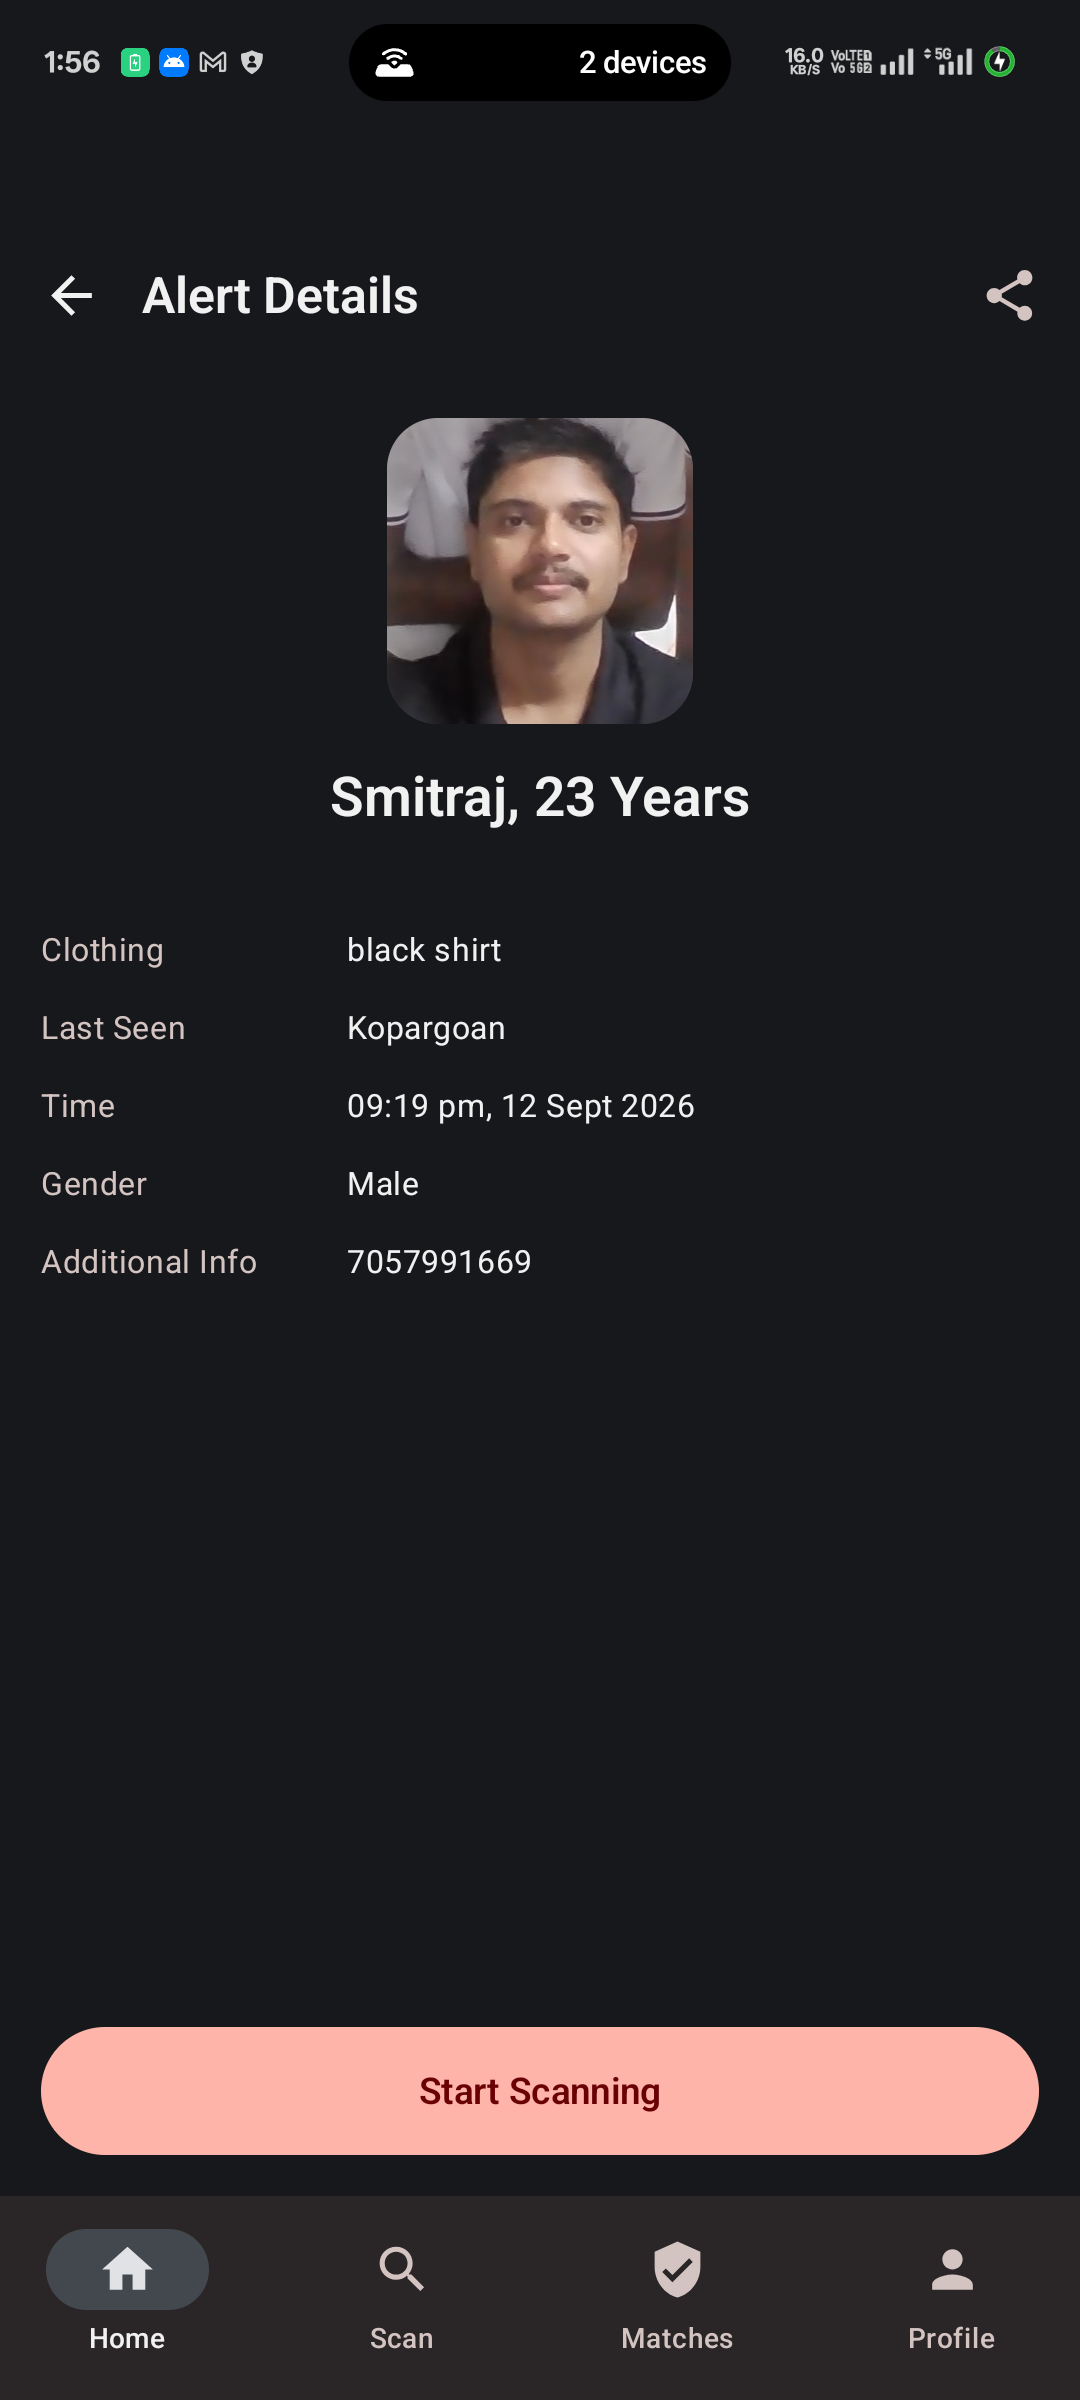
\includegraphics[width=\linewidth]{images/ss_05_alert_detail.png}
  \caption{Alert detail}
\end{subfigure}
\caption{Volunteer app -- sign-in and alert browsing}
\end{figure}

\begin{figure}[H]
\centering
\begin{subfigure}[t]{0.31\textwidth}
  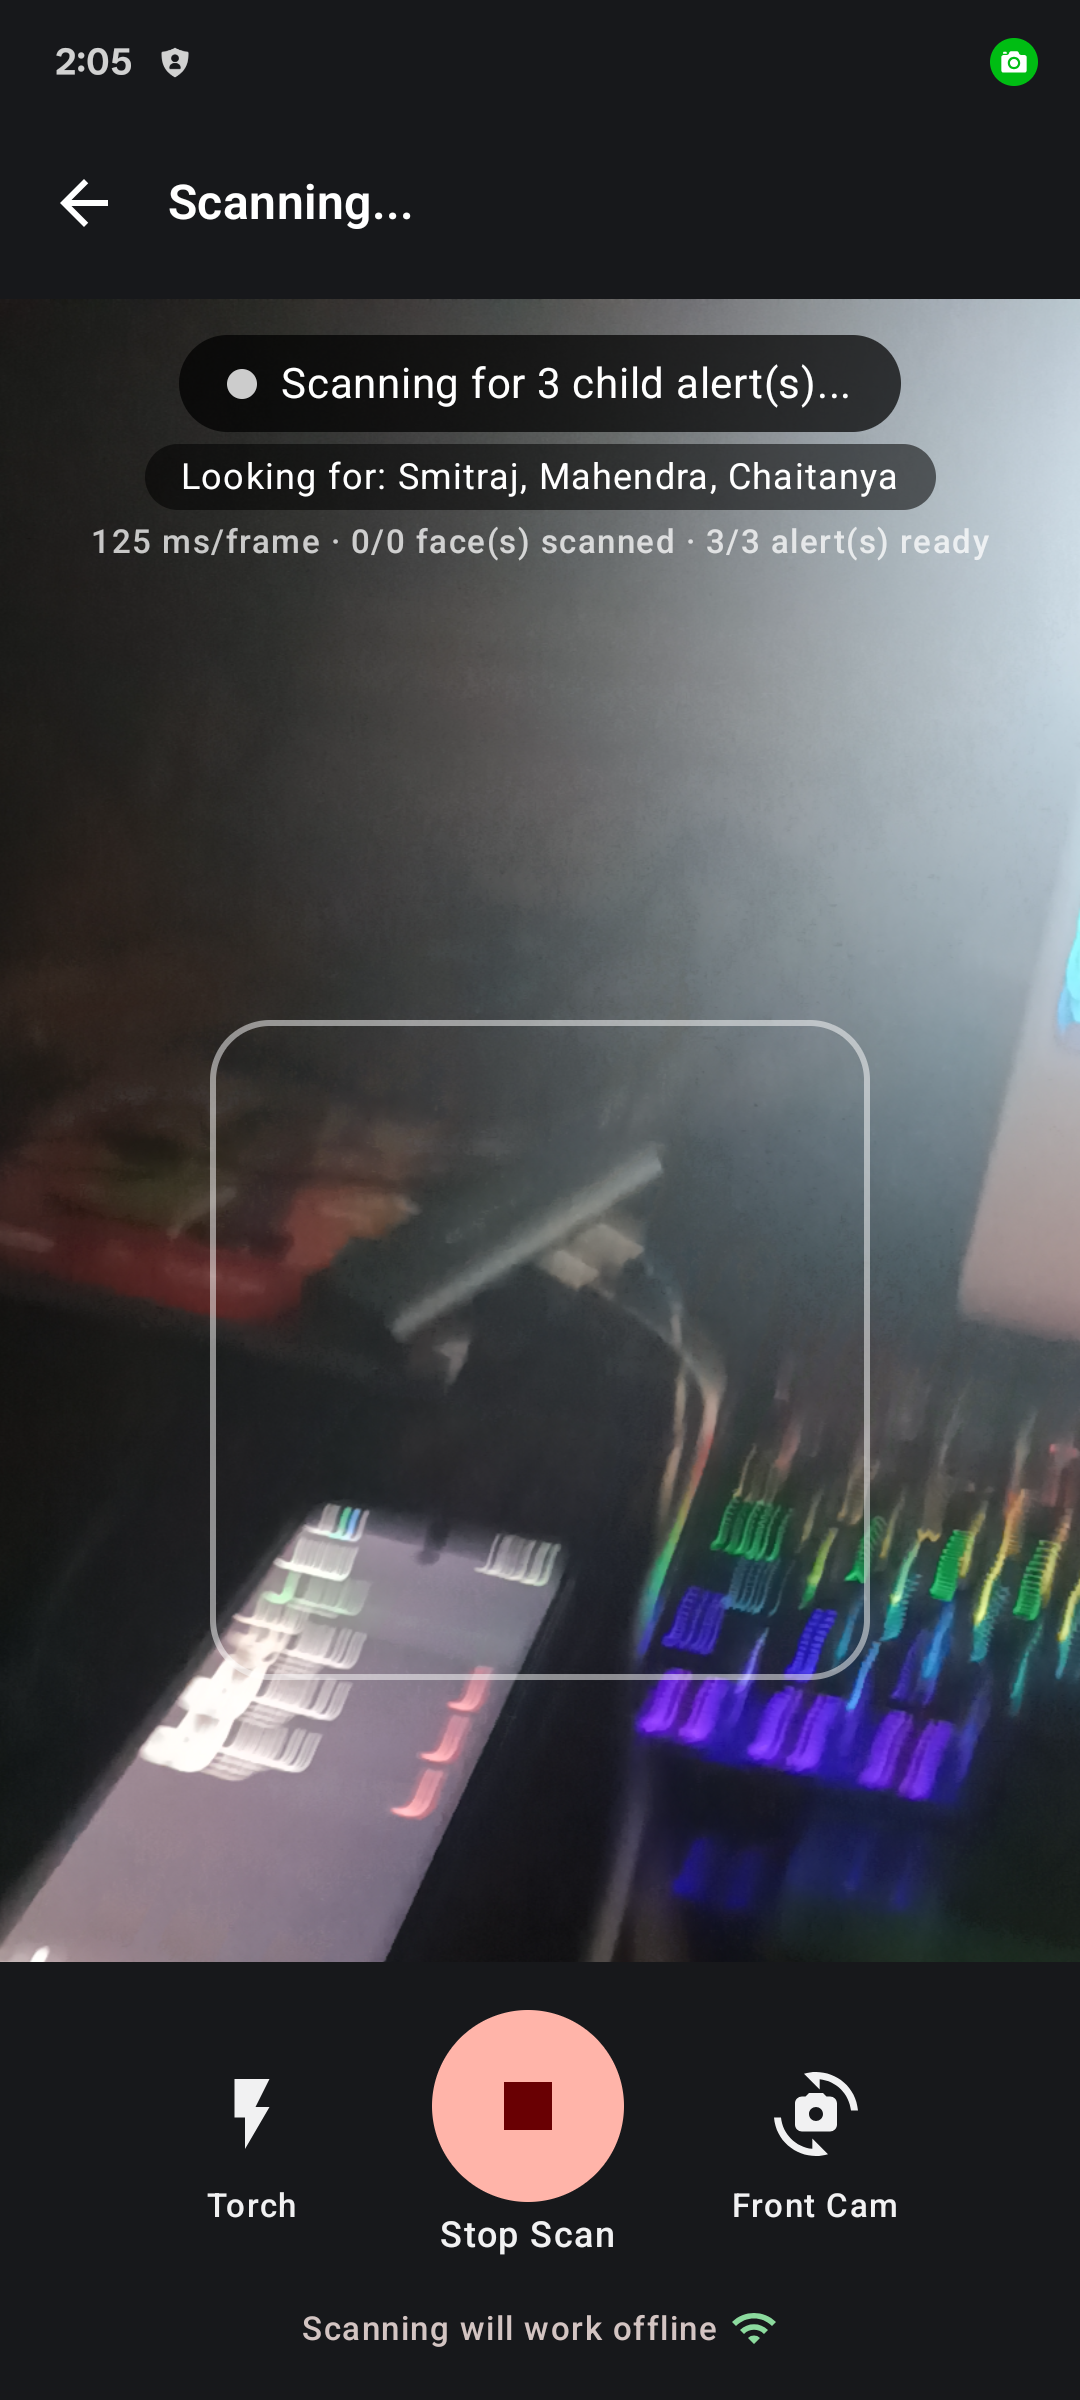
\includegraphics[width=\linewidth]{images/ss_06_scan.png}
  \caption{Live scan}
\end{subfigure}\hfill
\begin{subfigure}[t]{0.31\textwidth}
  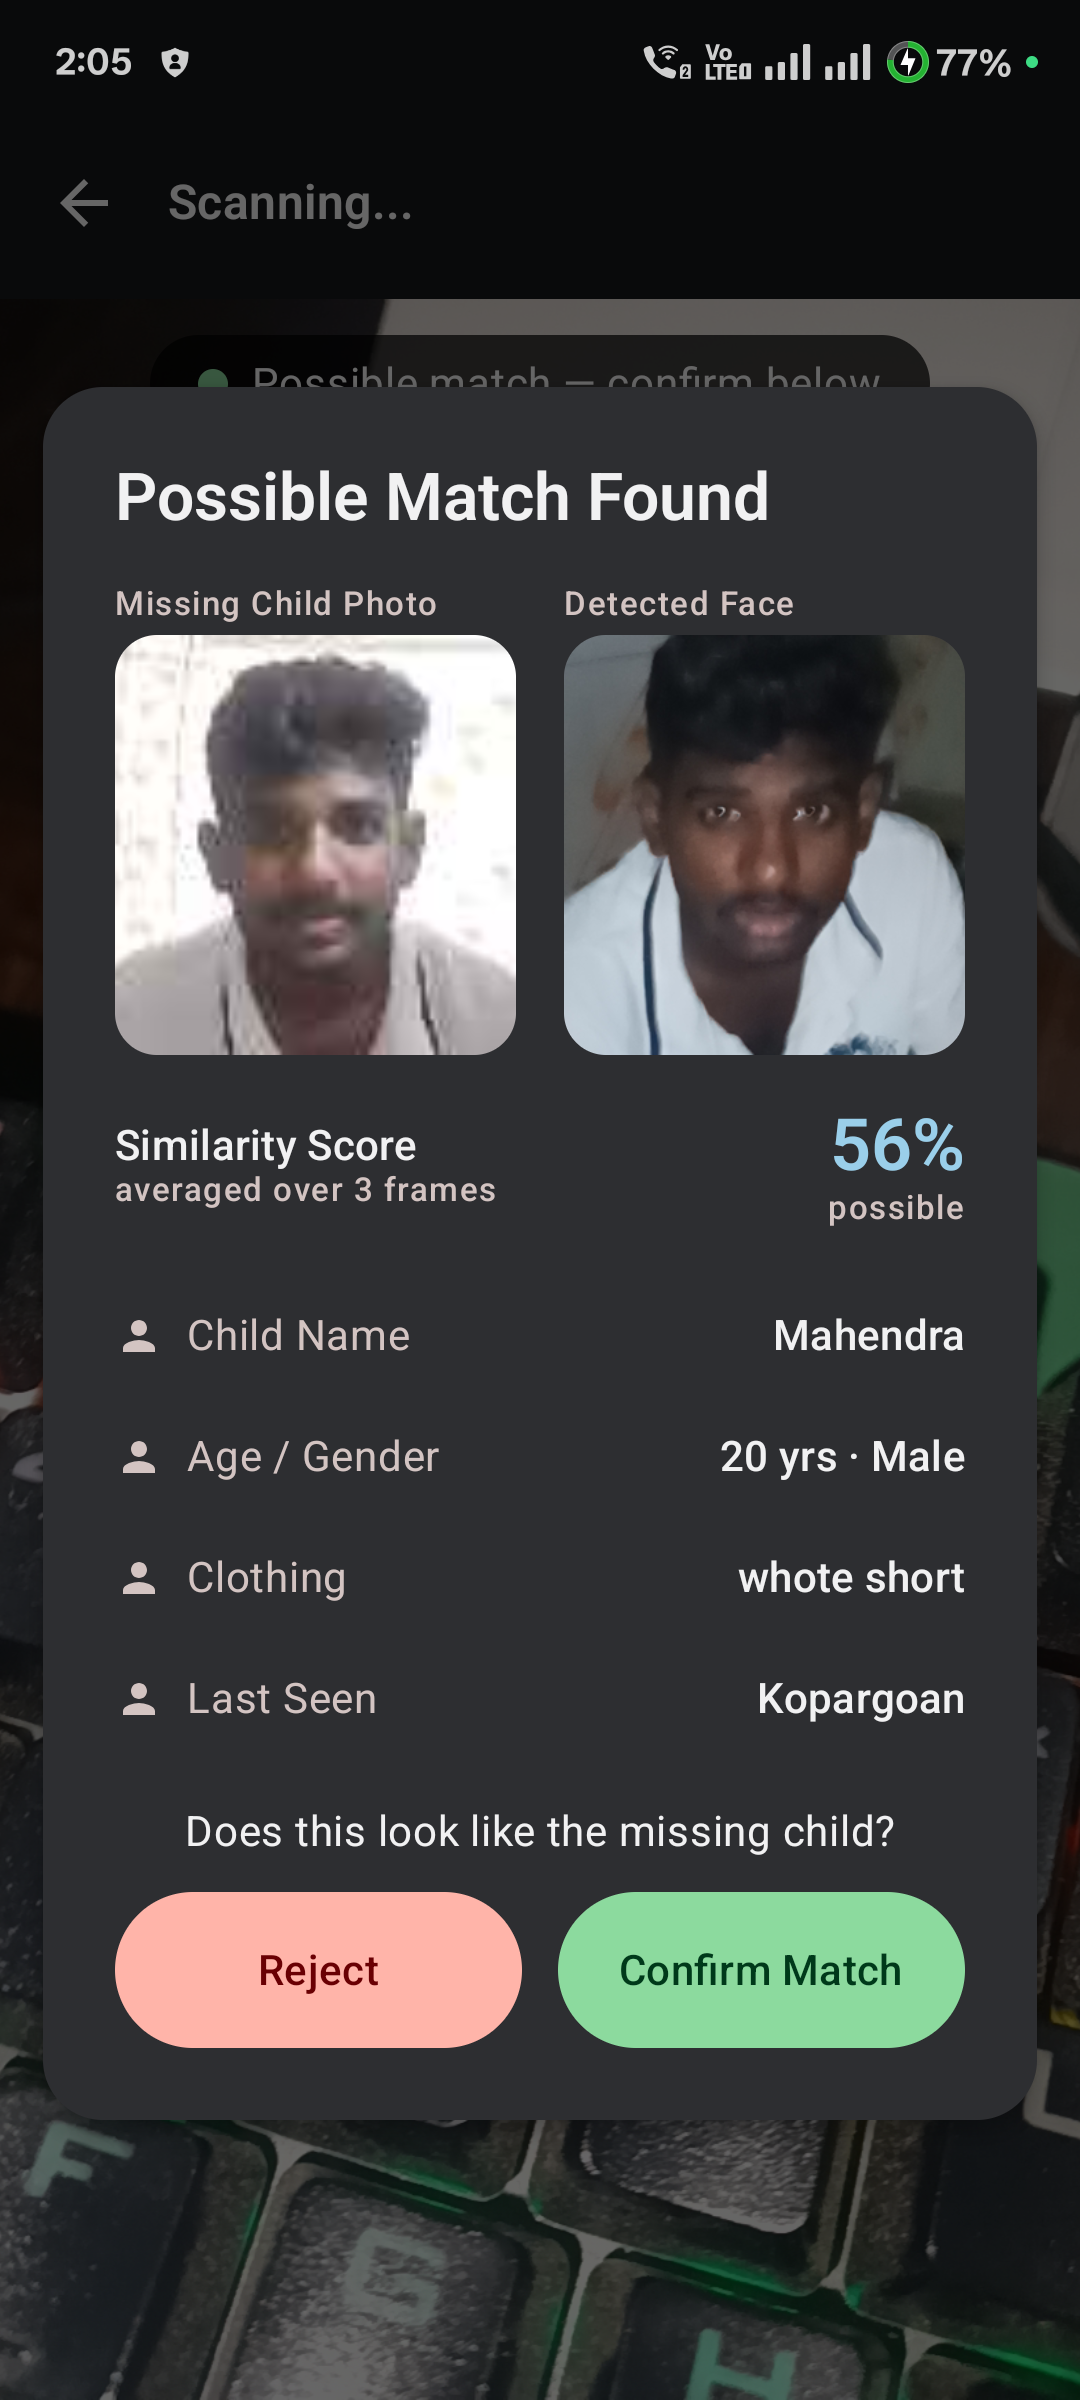
\includegraphics[width=\linewidth]{images/ss_07_match_popup.png}
  \caption{Candidate match dialog}
\end{subfigure}\hfill
\begin{subfigure}[t]{0.31\textwidth}
  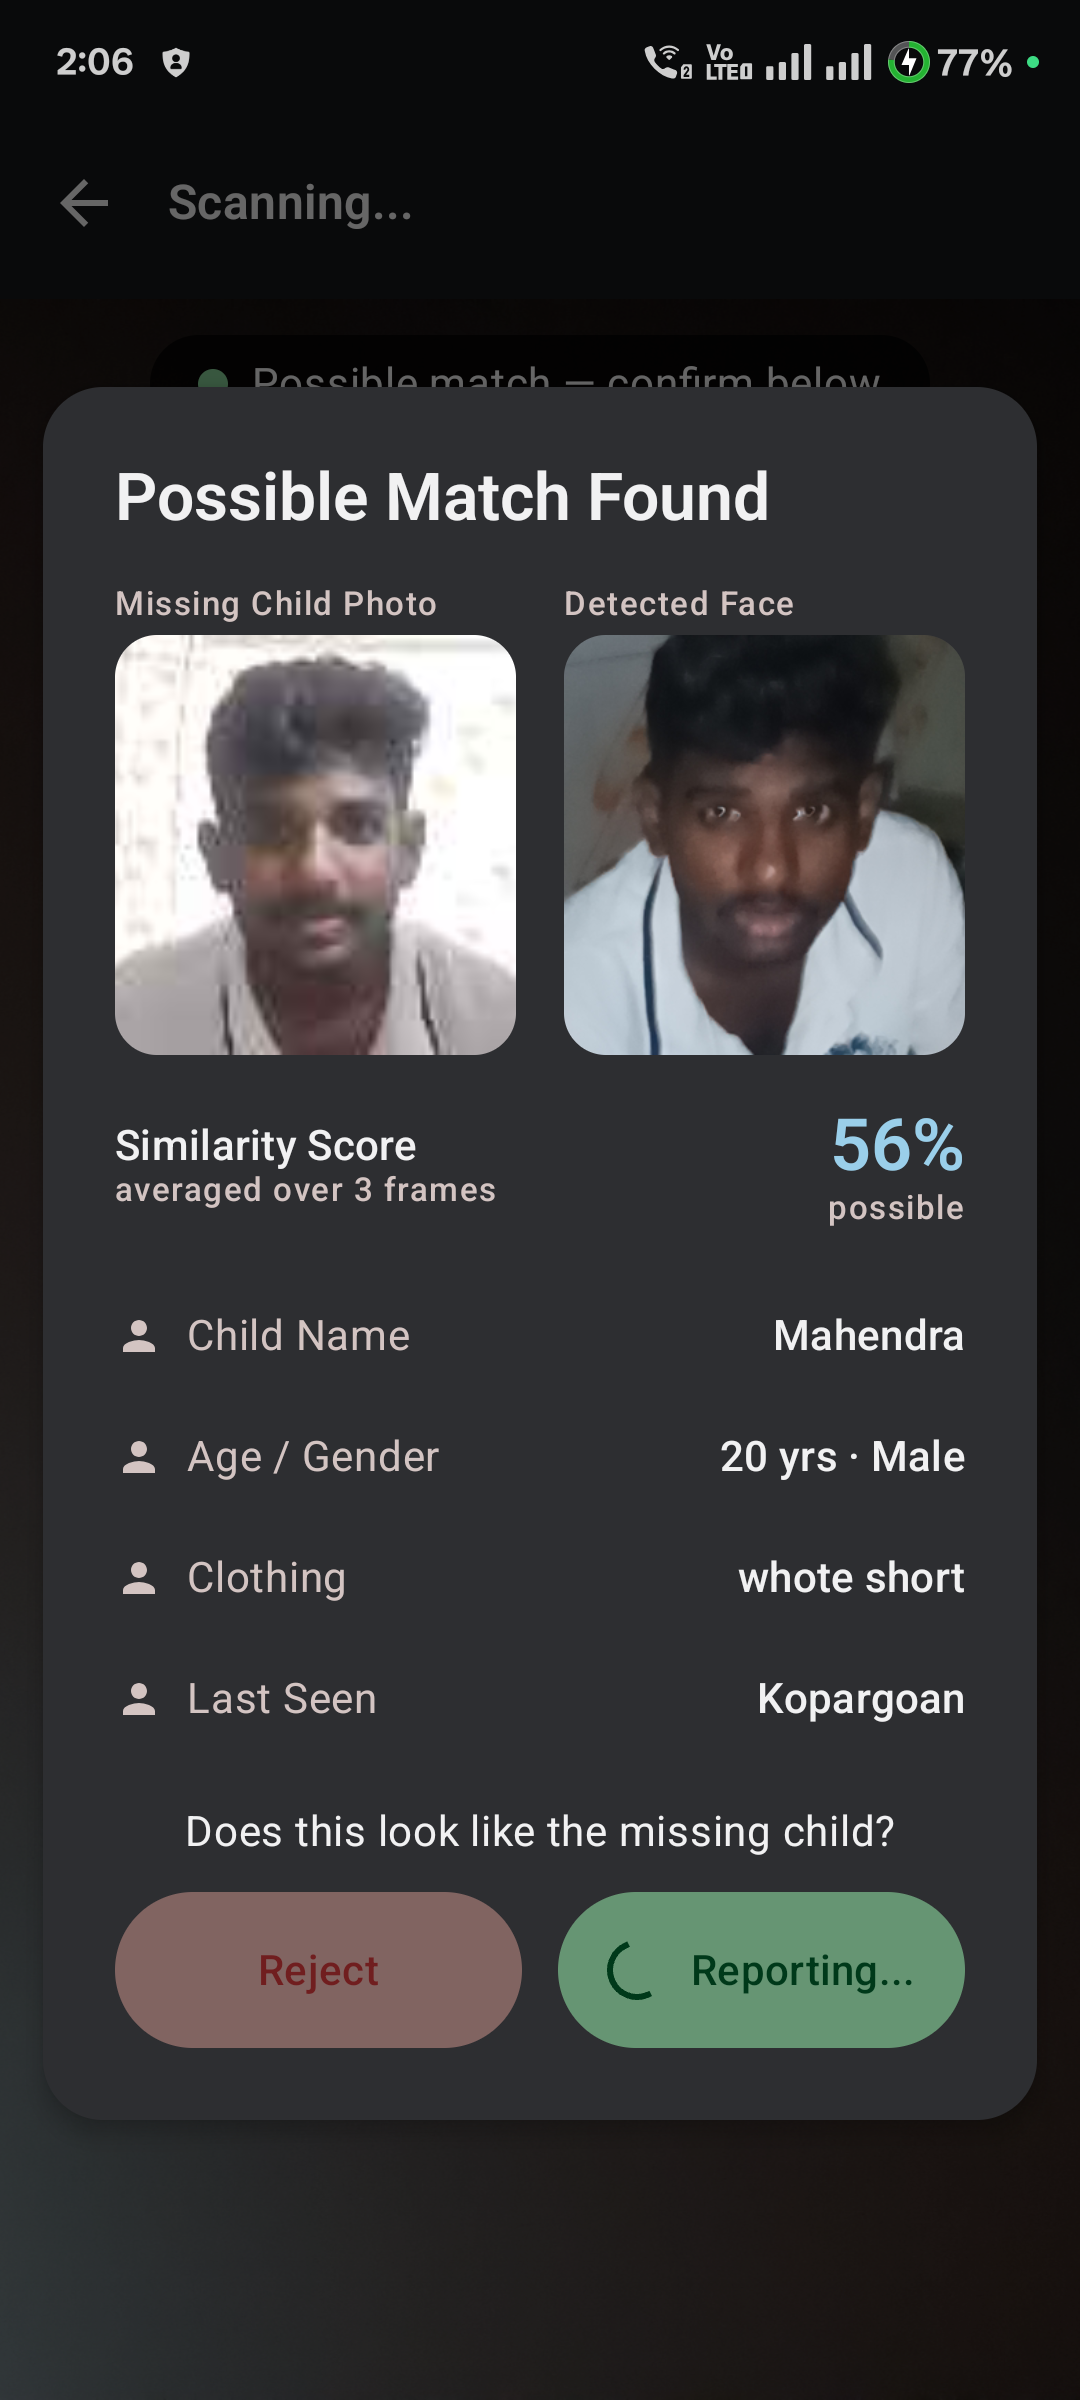
\includegraphics[width=\linewidth]{images/ss_08_confirming.png}
  \caption{Confirming a match}
\end{subfigure}
\caption{Volunteer app -- the core scan-and-confirm flow}
\end{figure}

\begin{figure}[H]
\centering
\begin{subfigure}[t]{0.31\textwidth}
  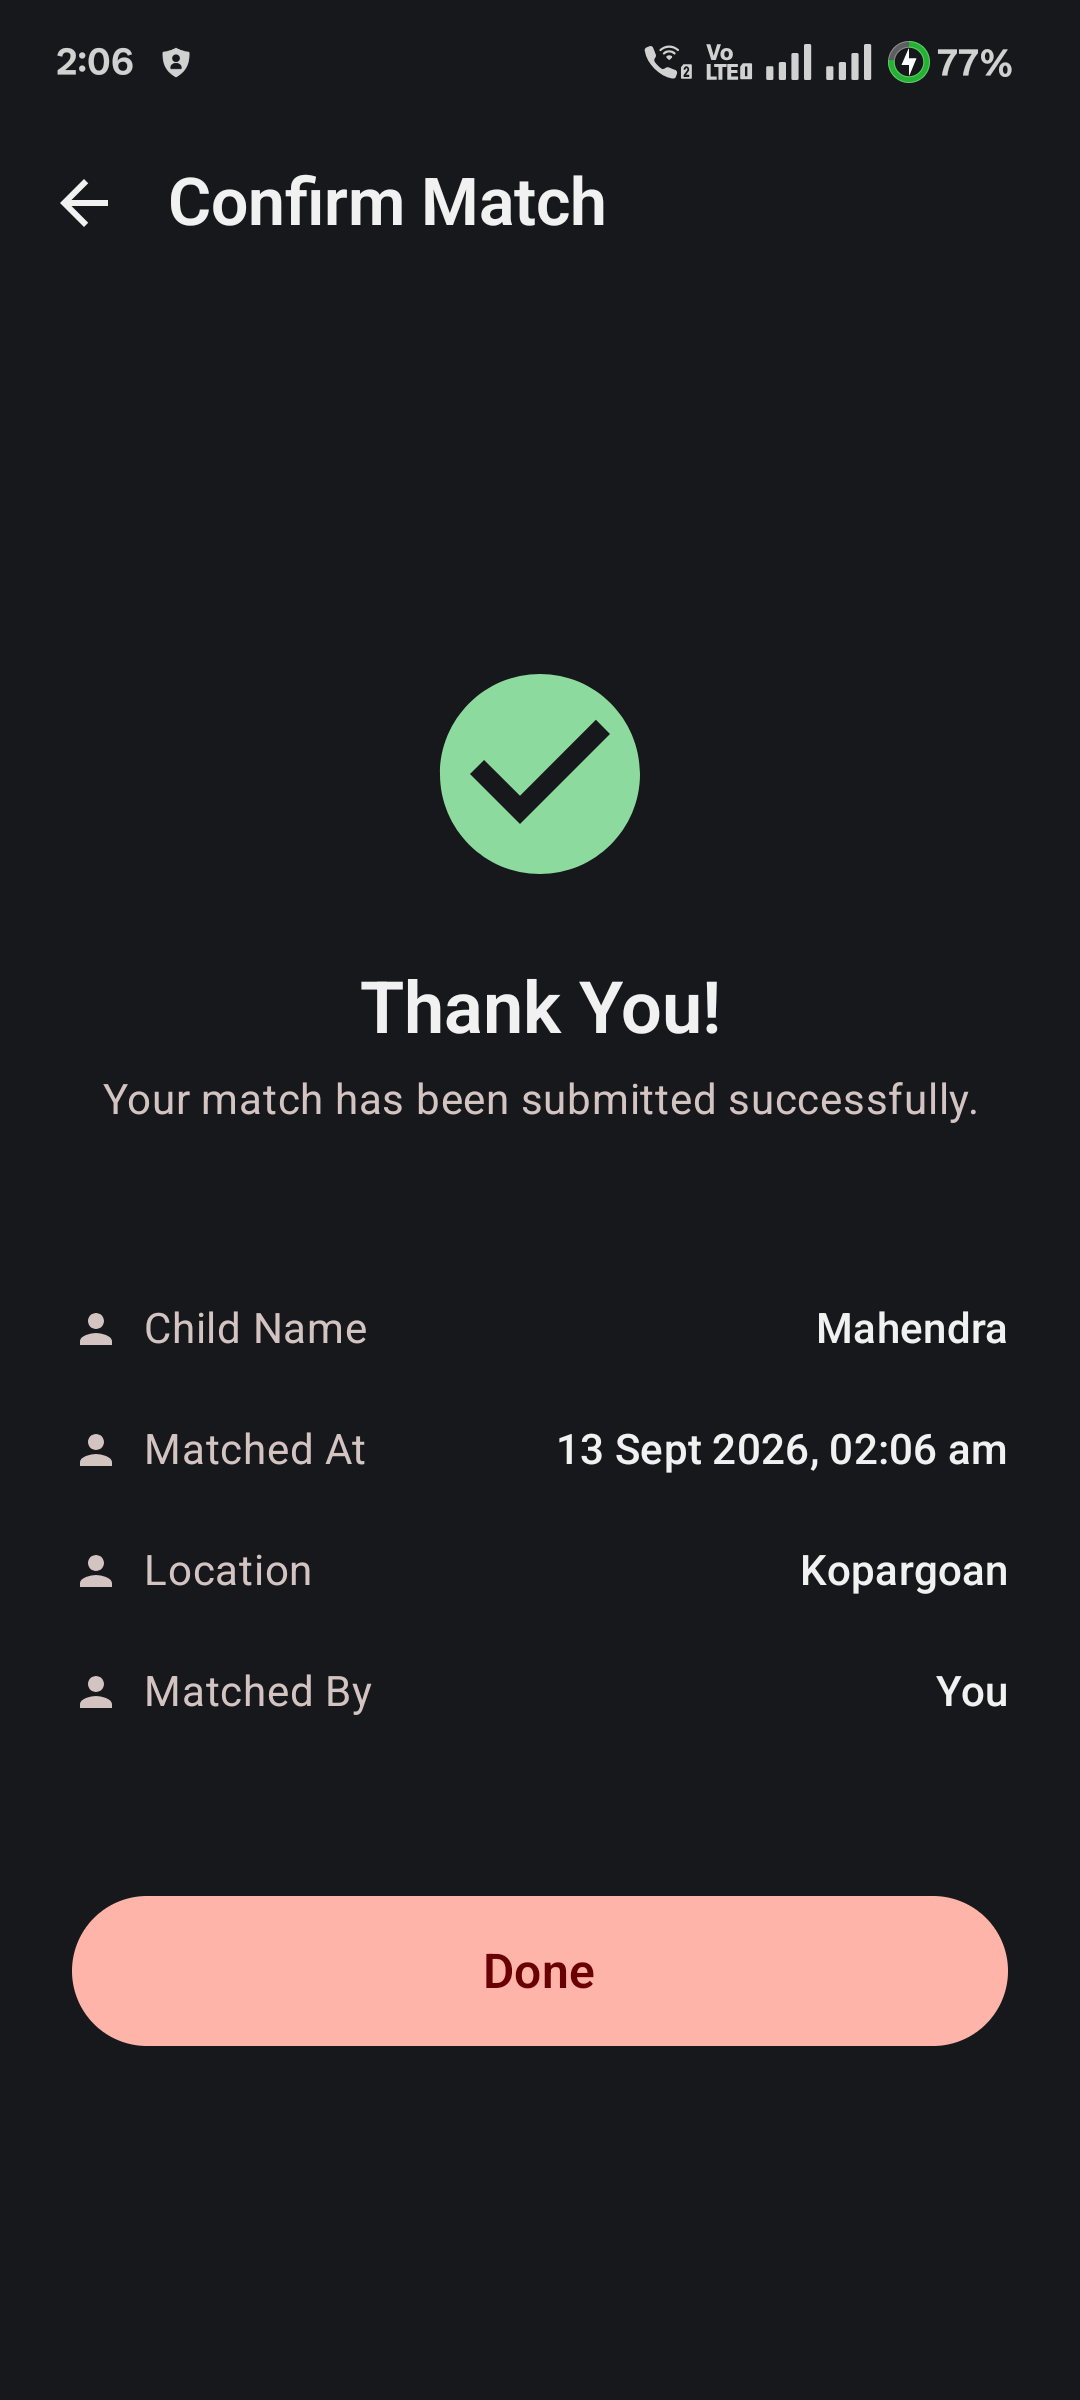
\includegraphics[width=\linewidth]{images/ss_09_thankyou.png}
  \caption{Match reported}
\end{subfigure}\hfill
\begin{subfigure}[t]{0.31\textwidth}
  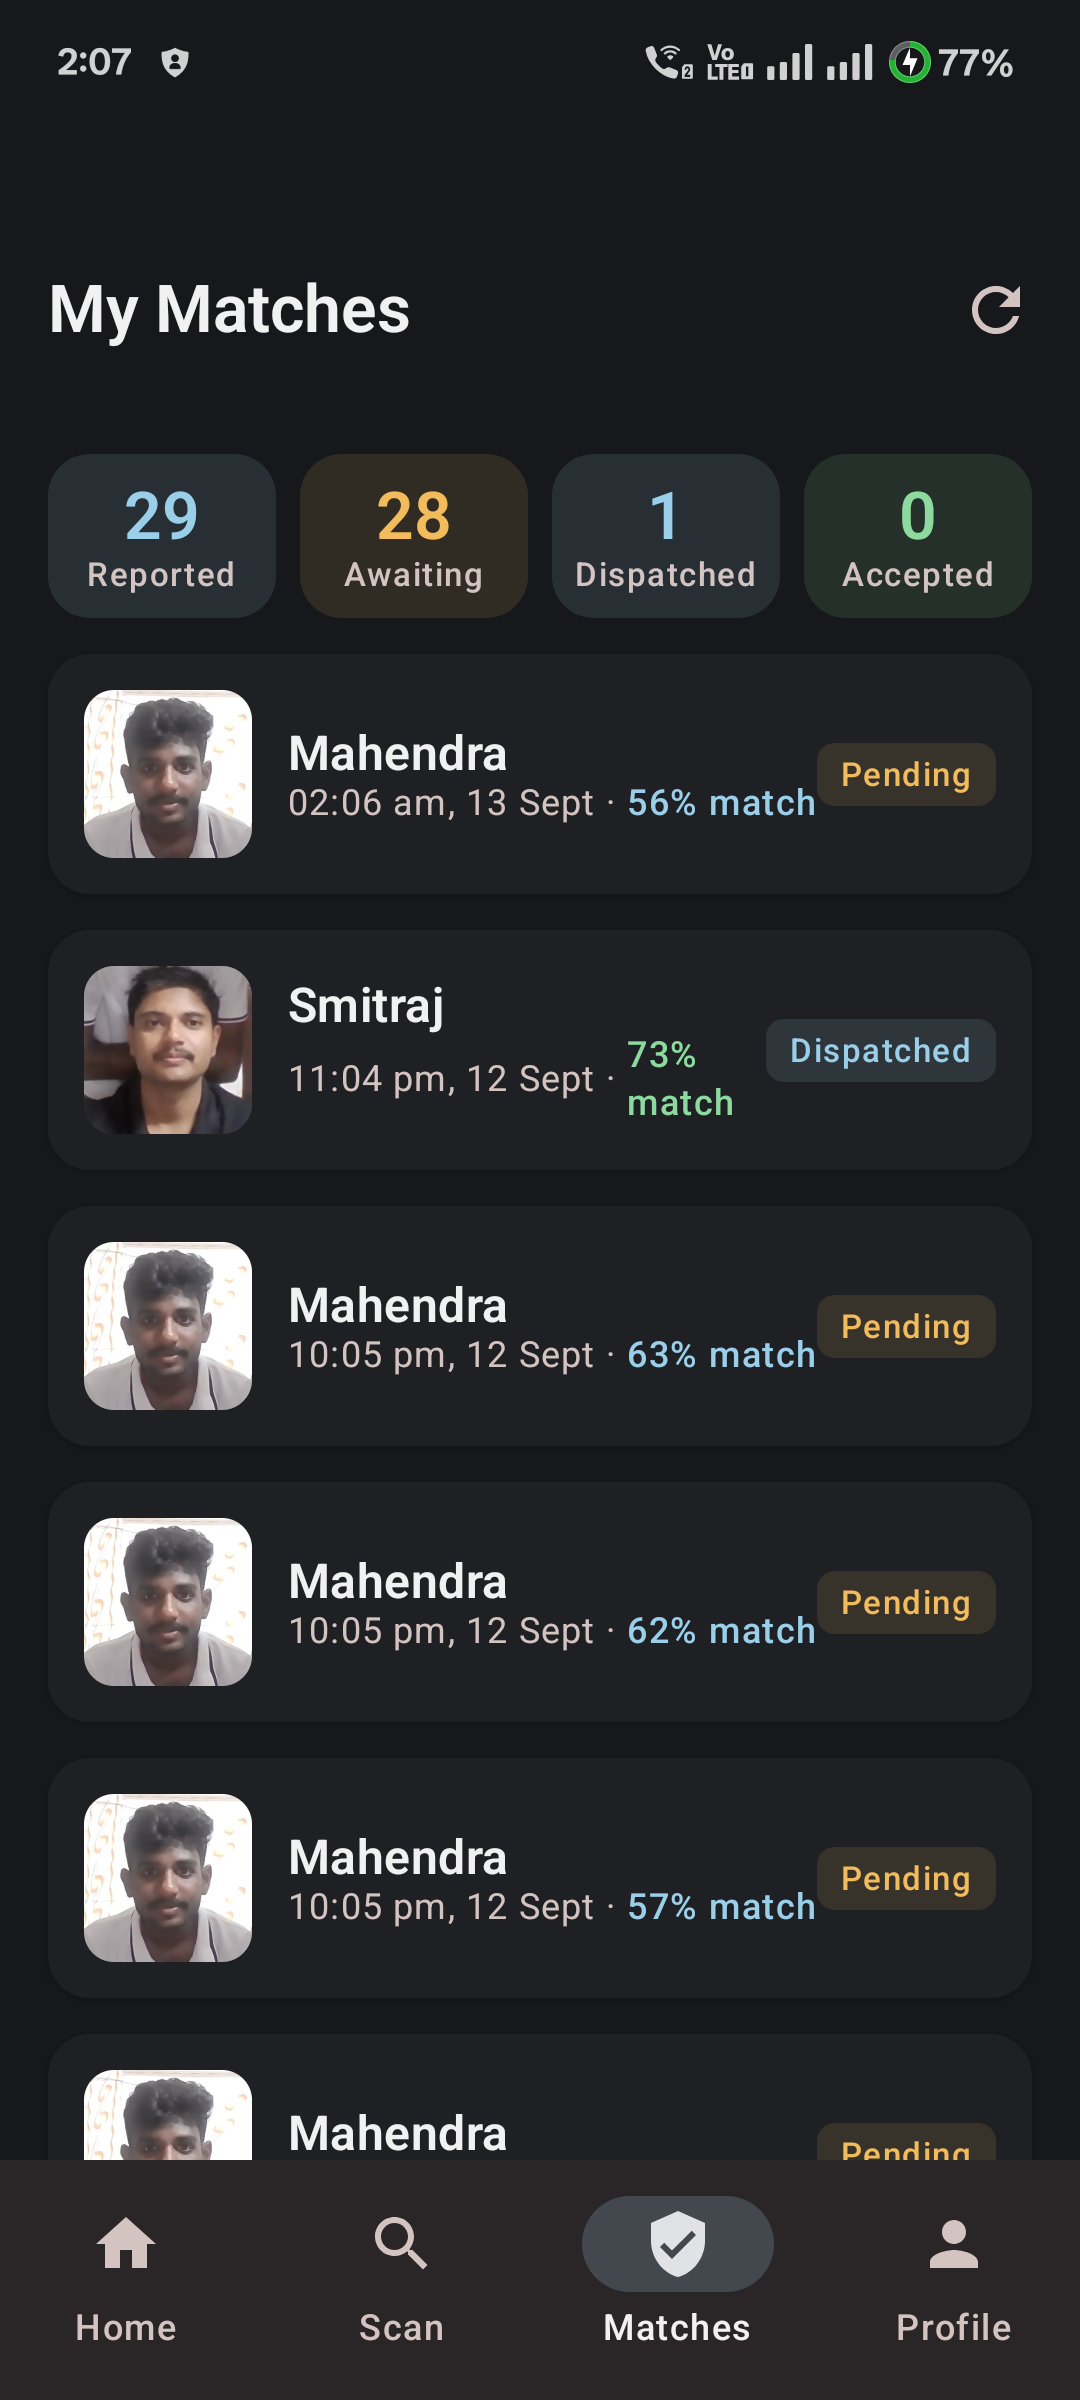
\includegraphics[width=\linewidth]{images/ss_11_matches.png}
  \caption{Volunteer's own match history}
\end{subfigure}\hfill
\begin{subfigure}[t]{0.31\textwidth}
  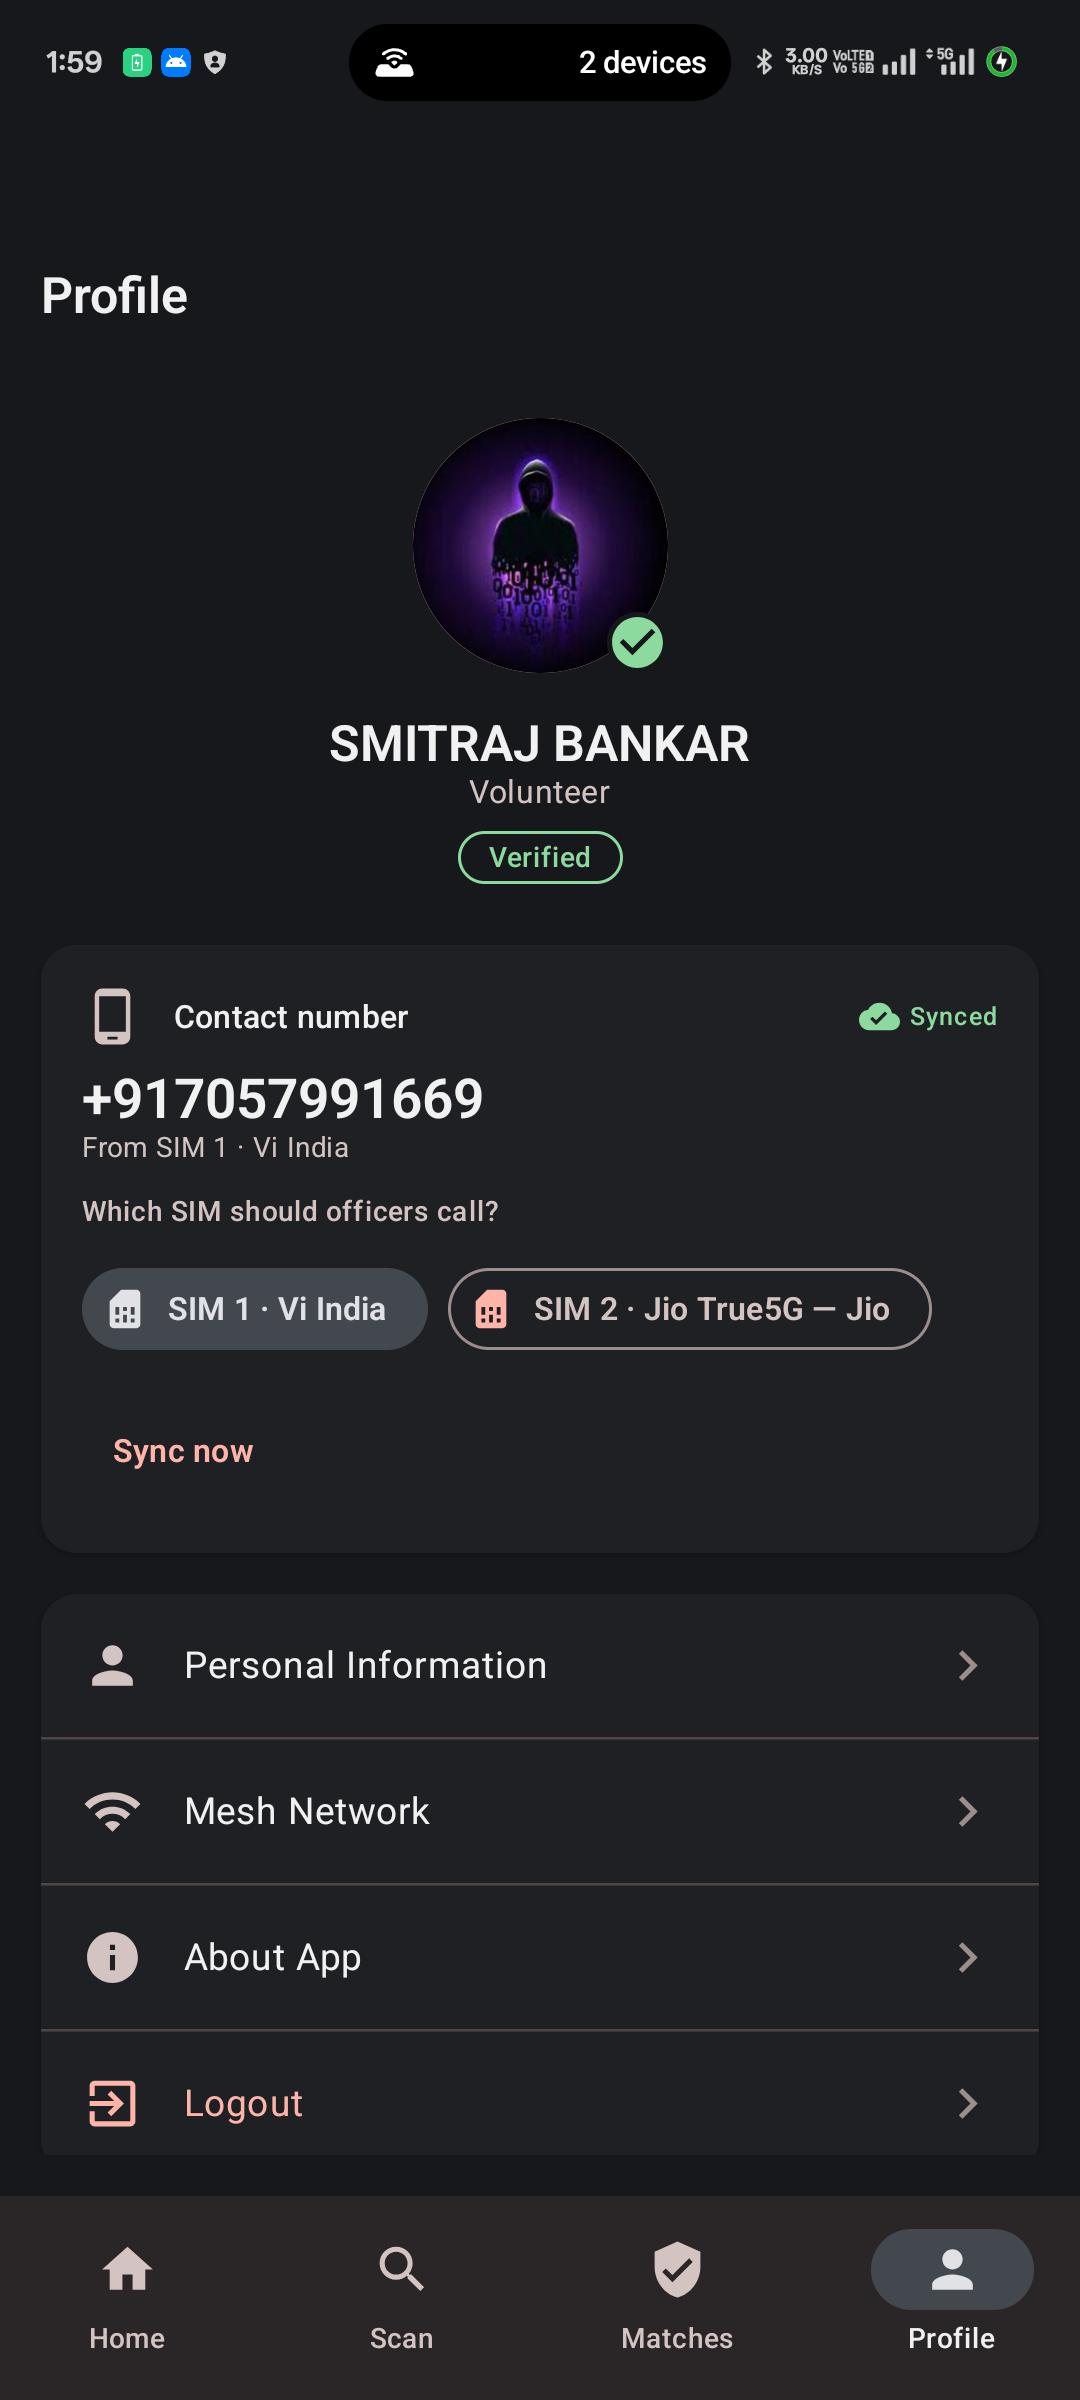
\includegraphics[width=\linewidth]{images/ss_13_profile.png}
  \caption{Profile}
\end{subfigure}
\caption{Volunteer app -- reporting confirmation, history, and profile}
\end{figure}

\subsection{Face Recognition Pipeline}

The pipeline is deliberately mirrored, field-for-field, across the Android
app, the Cloud Function, and the offline evaluation scripts, so that any two
implementations produce comparable embeddings:

\begin{enumerate}
  \item \textbf{Detect} -- Google ML Kit \cite{mlkit} locates faces and
        facial landmarks in each camera frame, tagging each detection with
        a stable tracking ID.
  \item \textbf{Frontality gate} -- faces with yaw beyond $40^\circ$ or roll
        beyond $35^\circ$ are rejected before any further processing.
  \item \textbf{3-point similarity alignment} -- the left eye, right eye,
        and nose landmarks are warped onto a canonical $112\times112$
        ArcFace \cite{arcface} template, so pose and scale differences are
        normalised out before embedding.
  \item \textbf{Quality gate} (device only) -- faces smaller than 48\,px,
        or with mean luma outside 25--240, or a Laplacian-variance sharpness
        below 12, are rejected as too small, too dark/bright, or too
        blurred to embed reliably.
  \item \textbf{Embed} -- the aligned $112\times112\times3$ tile is
        normalised to $[-1,1]$ and passed through the MobileFaceNet
        \cite{mobilefacenet} TFLite \cite{tflite} interpreter, producing an
        L2-normalised embedding vector.
  \item \textbf{Multi-frame fusion} -- up to three embeddings per tracked
        face are averaged, gated by a coherence floor so a recycled
        tracking ID cannot blend two different people's embeddings.
  \item \textbf{Cosine compare} -- the fused embedding is compared against
        every currently active alert's embedding.
\end{enumerate}

\begin{lstlisting}[language=Kotlin, caption={Cosine similarity comparator -- \texttt{domain/\allowbreak matching/\allowbreak CosineEmbeddingComparator.kt}}]
class CosineEmbeddingComparator : EmbeddingComparator {
    override fun similarity(a: FloatArray, b: FloatArray): Float {
        require(a.size == b.size) { "Embedding width mismatch" }
        var dot = 0f
        for (i in a.indices) dot += a[i] * b[i]
        // Both vectors are L2-normalised at embedding time,
        // so the dot product alone equals cosine similarity.
        return dot.coerceIn(-1f, 1f)
    }
}
\end{lstlisting}

\begin{lstlisting}[language=Kotlin, caption={Match decision constants -- \texttt{utils/Constants.kt} (excerpt)}]
object Constants {
    const val SIMILARITY_THRESHOLD = 0.55f      // measured, not assumed
    const val STRONG_MATCH_THRESHOLD = 0.72f    // instant single-frame match
    const val MATCH_CONFIRM_FRAMES = 2          // mid-band confirmation
    const val EMBEDDING_FUSION_FRAMES = 3
    const val TRACK_COHERENCE_MIN = 0.5f
    const val FACE_CROP_MARGIN = 0.2f
}
\end{lstlisting}

\subsection{Alert embeddings are recomputed on-device}
\label{sec:reembed}

A key correctness fix discovered during testing: the phone re-embeds the
alert's own photograph with its own model at scan time, rather than trusting
the server's embedding directly. Measurement showed that comparing an
embedding produced by one geometry pipeline (a centred crop) against one
produced by another (3-point alignment) scores the \emph{same face} at
0.38--0.49 -- below the 0.55 threshold -- even though the two photos are of
the same person. Mixing geometries does not degrade matching gracefully; it
silently disables it. Re-embedding on-device removes this failure class
entirely, since both sides of every comparison now come from one
implementation.

\subsection{Face-Match Threshold: Measured, Not Assumed}
\label{sec:threshold-measurement}

The synopsis originally assumed a cosine threshold of 0.75, taken from
general face-recognition literature rather than from this model on this
pipeline. It was re-measured directly, and the measurement changed the
number:

\begin{table}[H]
\centering
\caption{Threshold measurement -- 36 labelled real pairs, original unaligned MobileFaceNet}
\begin{tabular}{|p{5.4cm}|p{5.4cm}|}
\hline
\textbf{Same-person pairs} & \textbf{Different-person pairs} \\
\hline
Cosine score range: 0.7142 -- 0.9899 & Cosine score range: 0.0864 -- 0.3551 \\
\hline
\end{tabular}
\end{table}

The two ranges leave an empty band from 0.3551 to 0.7142 with no observed
pairs at all; \code{SIMILARITY\_THRESHOLD = 0.55} was set near the middle
of that gap. The synopsis's original 0.75 sits \emph{inside} the genuine-pair
range above -- at that value the system would have rejected several true
matches as non-matches. This is the concrete reason the team's engineering
policy is to re-measure after any change to the model, the alignment, or
the TFLite precision, rather than trust a literature default -- a policy
this exact number already justified once.

\begin{table}[H]
\centering
\caption{Geometry parity -- same photo, same identity, different alignment pipelines}
\begin{tabular}{|p{7.0cm}|p{3.8cm}|}
\hline
\textbf{Pairing} & \textbf{Cosine score} \\
\hline
Centred crop vs.\ centred crop & 0.8855 \\ \hline
3-point alignment vs.\ 3-point alignment & 0.8467 \\ \hline
Centred crop vs.\ 3-point alignment (\emph{same} photo, mismatched geometry) & 0.38 -- 0.49 \\
\hline
\end{tabular}
\end{table}

This is the measurement behind \S\ref{sec:reembed}'s re-embedding decision: mixing two
correct alignment geometries scores an \emph{identical} face below the 0.55
threshold. A geometry mismatch does not degrade matching gracefully -- it
silently disables it, which is far more dangerous than an obvious crash
because nothing in the UI indicates a fault has occurred.

\subsection{Concurrency Safety on the Interpreter Thread}
\label{sec:concurrency-safety}

The TFLite interpreter is not safe to call from two frames at once. It runs
on a single dedicated thread (XNNPACK, 4 threads internally), and every
call into it is gated by an \code{AtomicBoolean}: if a frame arrives while
the previous one is still being embedded, it is dropped rather than queued
behind the interpreter. A race in this exact gate -- traceable to commit
\texttt{bb0f829} (Table~\ref{tab:commits}) -- was the ``model deadlock''
found during the final week of real-device testing (\S\ref{sec:weekly-log}): under
sustained load the interpreter could be entered twice, and the second call
would block forever waiting on a lock the first call already held. It
surfaced only on physical hardware under continuous scanning, never on the
emulator or in a unit test, which is why the fix landed in the project's
final week rather than earlier.

\subsection{Local Persistence and Background Sync}

A confirmed match must survive a dropped connection, a killed process, or
a phone that is genuinely offline for the rest of the event. Reports are
therefore never held only in memory: \code{ReportMatchUseCase} always
writes to a Room database first, and network delivery happens
asynchronously from that durable queue.

\begin{lstlisting}[language=Kotlin, caption={Pending-match entity and DAO -- \texttt{data/local/PendingMatchEntity.kt} (excerpt)}]
@Entity(tableName = "pending_matches")
data class PendingMatchEntity(
    @PrimaryKey val id: String,           // client-generated UUID
    val alertId: String,
    val confidence: Float,
    val latitude: Double?,
    val longitude: Double?,
    val sightingPhotoPath: String,
    val status: String,                   // QUEUED | SYNCED | RELAYED
    val createdAt: Long,
)

@Dao
interface PendingMatchDao {
    @Insert suspend fun insert(entity: PendingMatchEntity)
    @Query("SELECT * FROM pending_matches WHERE status = 'QUEUED'")
    suspend fun queued(): List<PendingMatchEntity>
    @Update suspend fun update(entity: PendingMatchEntity)
}
\end{lstlisting}

\code{MatchSyncWorker}, a connectivity-gated \code{WorkManager} job, drains
this queue whenever the device regains a network path -- including a path
that only just opened because a mesh peer came online. \code{AppDatabase}
is versioned (currently v4); each schema change (adding the mesh tables,
then the thumbnail column, then the gateway-routing fields) shipped its own
\code{Migration}, so an upgrading install never loses a volunteer's
already-queued reports.

\begin{lstlisting}[language=Kotlin, caption={Connectivity-gated sync -- \texttt{networking/MatchSyncWorker.kt} (excerpt)}]
class MatchSyncWorker(ctx: Context, params: WorkerParameters) :
    CoroutineWorker(ctx, params) {

    override suspend fun doWork(): Result {
        val queued = pendingMatchDao.queued()
        queued.forEach { pending ->
            val uploaded = matchRepository.upload(pending)
            if (uploaded) pendingMatchDao.update(pending.copy(status = "SYNCED"))
        }
        return Result.success()
    }

    companion object {
        fun enqueue(ctx: Context) {
            val constraints = Constraints.Builder()
                .setRequiredNetworkType(NetworkType.CONNECTED)
                .build()
            val request = OneTimeWorkRequestBuilder<MatchSyncWorker>()
                .setConstraints(constraints)
                .build()
            WorkManager.getInstance(ctx).enqueue(request)
        }
    }
}
\end{lstlisting}

The volunteer's own profile (name, phone, cached avatar URL) is kept in a
separate \code{DataStore}-backed \code{VolunteerStore}, not Room -- a
single small object with no query needs, refreshed from the SIM
(\code{SimPhoneProvider}) every time the Profile screen opens so the
number an officer would call is always current.

\section{Complete End-to-End Mobile Application Workflow}

To document the volunteer app as it actually behaves rather than in
isolated fragments, Figures~\ref{fig:wf1}--\ref{fig:wf7} walk through all
nineteen screens of one continuous session on real hardware, in the exact
order they occur: signing in, receiving and reading an alert, scanning and
confirming a live match, reviewing match history, managing the profile and
the offline mesh, and signing out.

\begin{figure}[H]
\centering
\begin{subfigure}[t]{0.31\textwidth}
  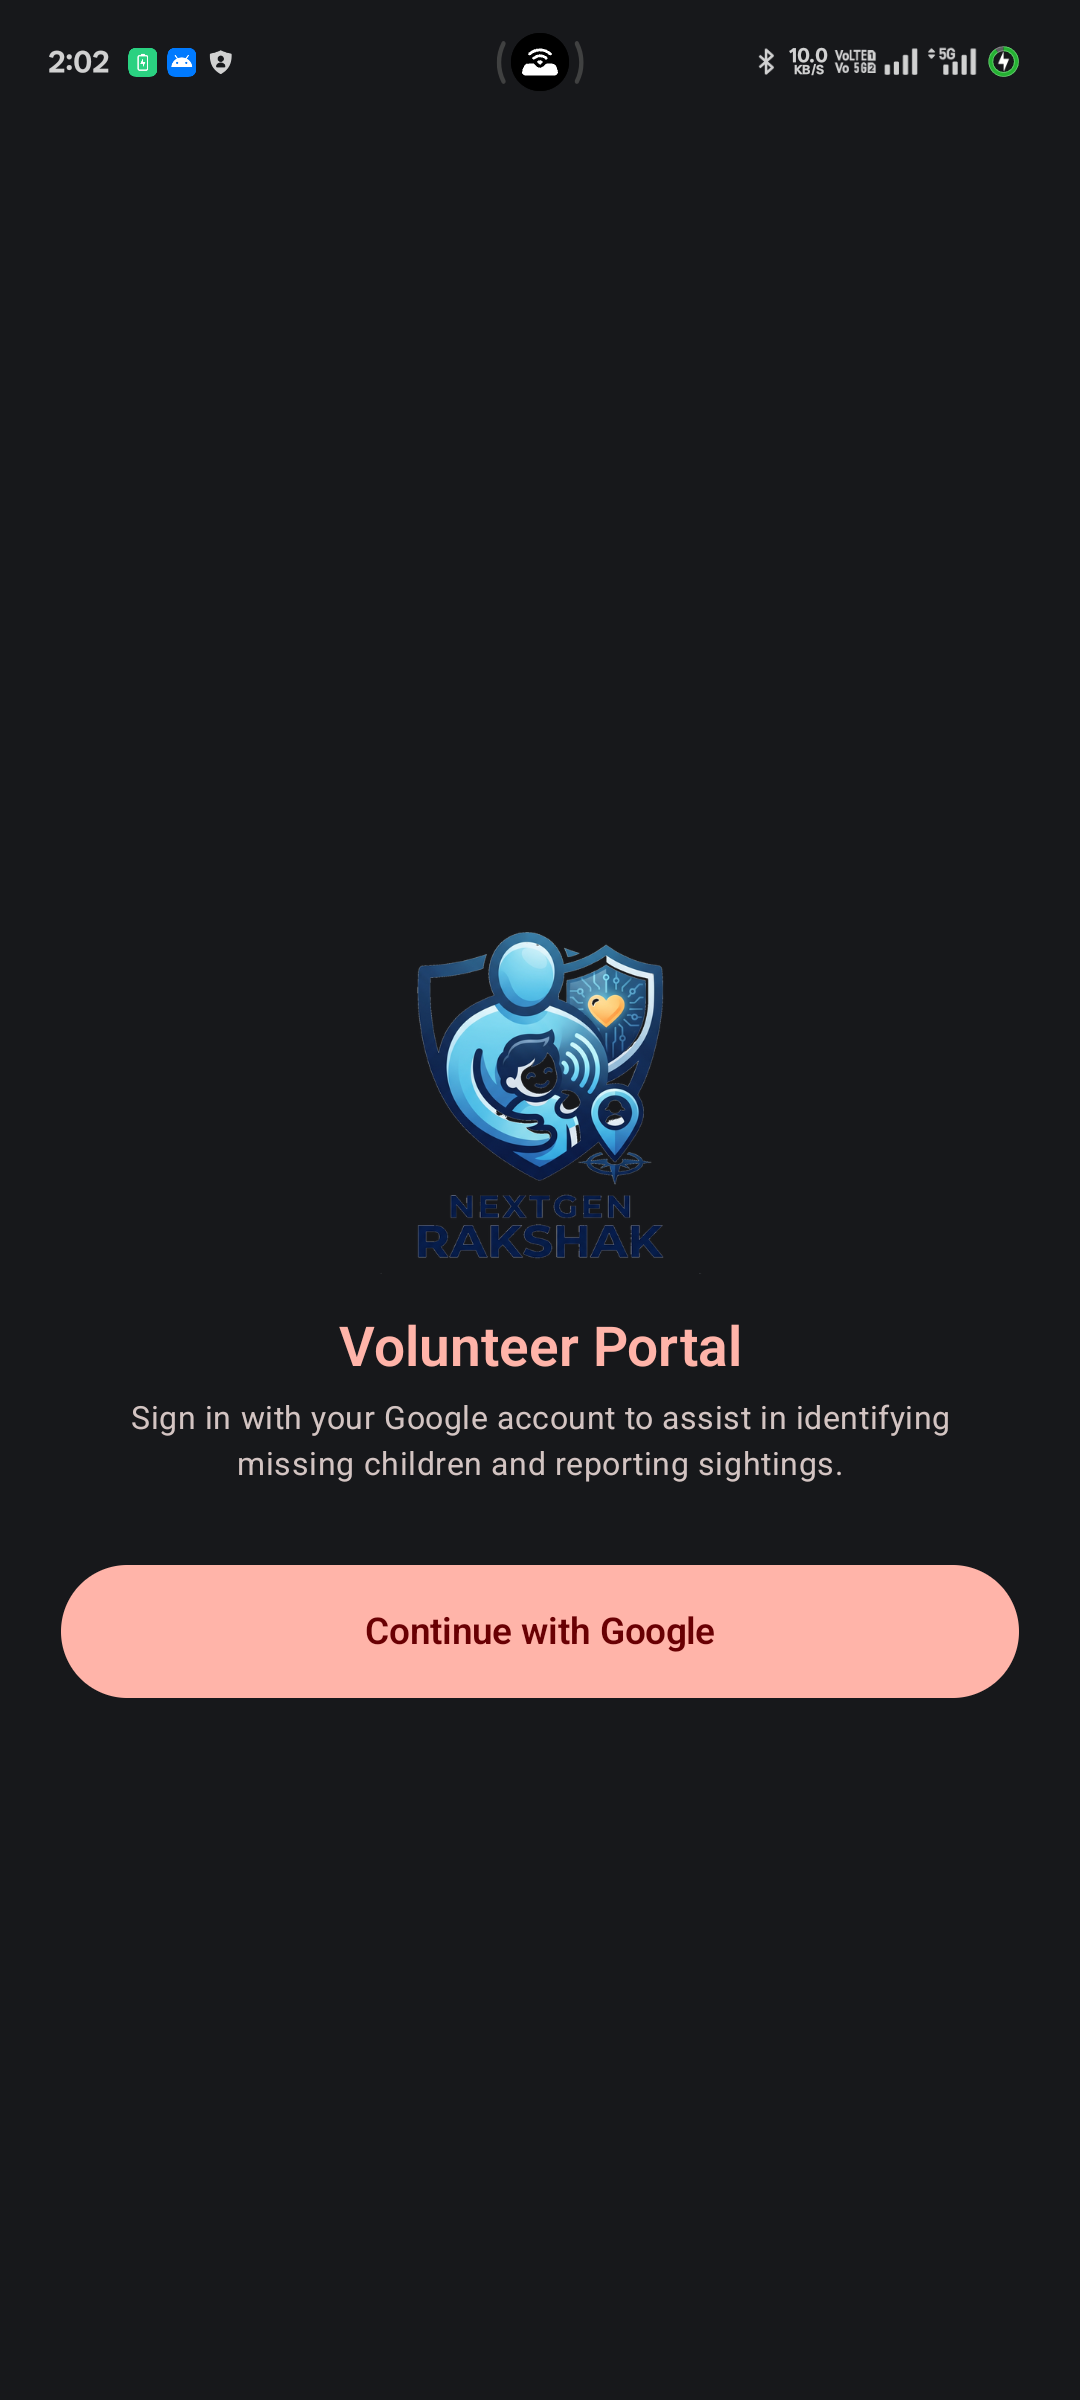
\includegraphics[width=\linewidth]{images/ss_01_login.png}
  \caption{1. Login screen}
\end{subfigure}\hfill
\begin{subfigure}[t]{0.31\textwidth}
  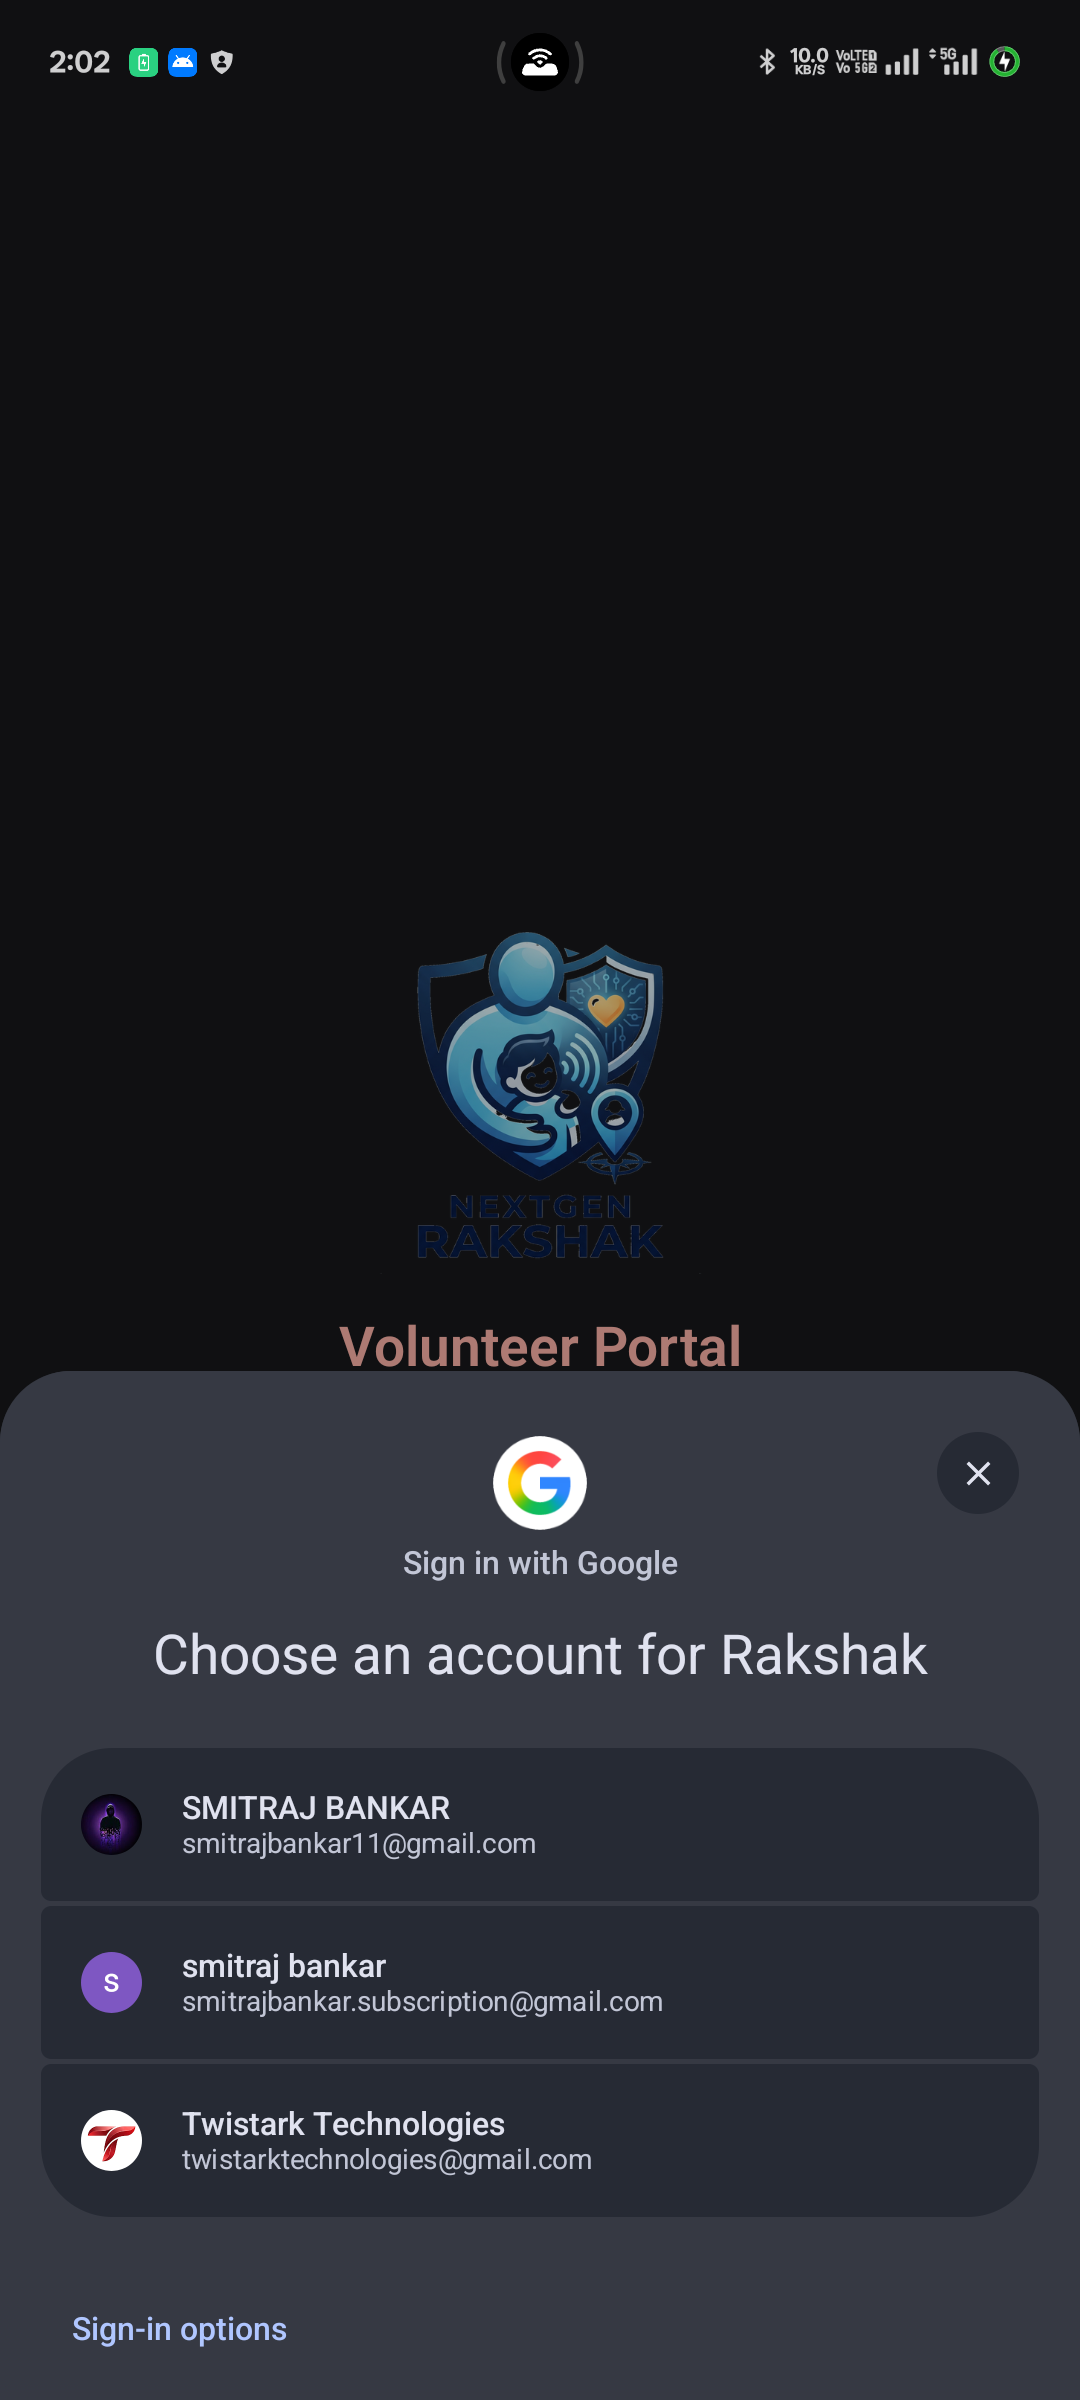
\includegraphics[width=\linewidth]{images/ss_02_google_picker.png}
  \caption{2. Google account picker}
\end{subfigure}\hfill
\begin{subfigure}[t]{0.31\textwidth}
  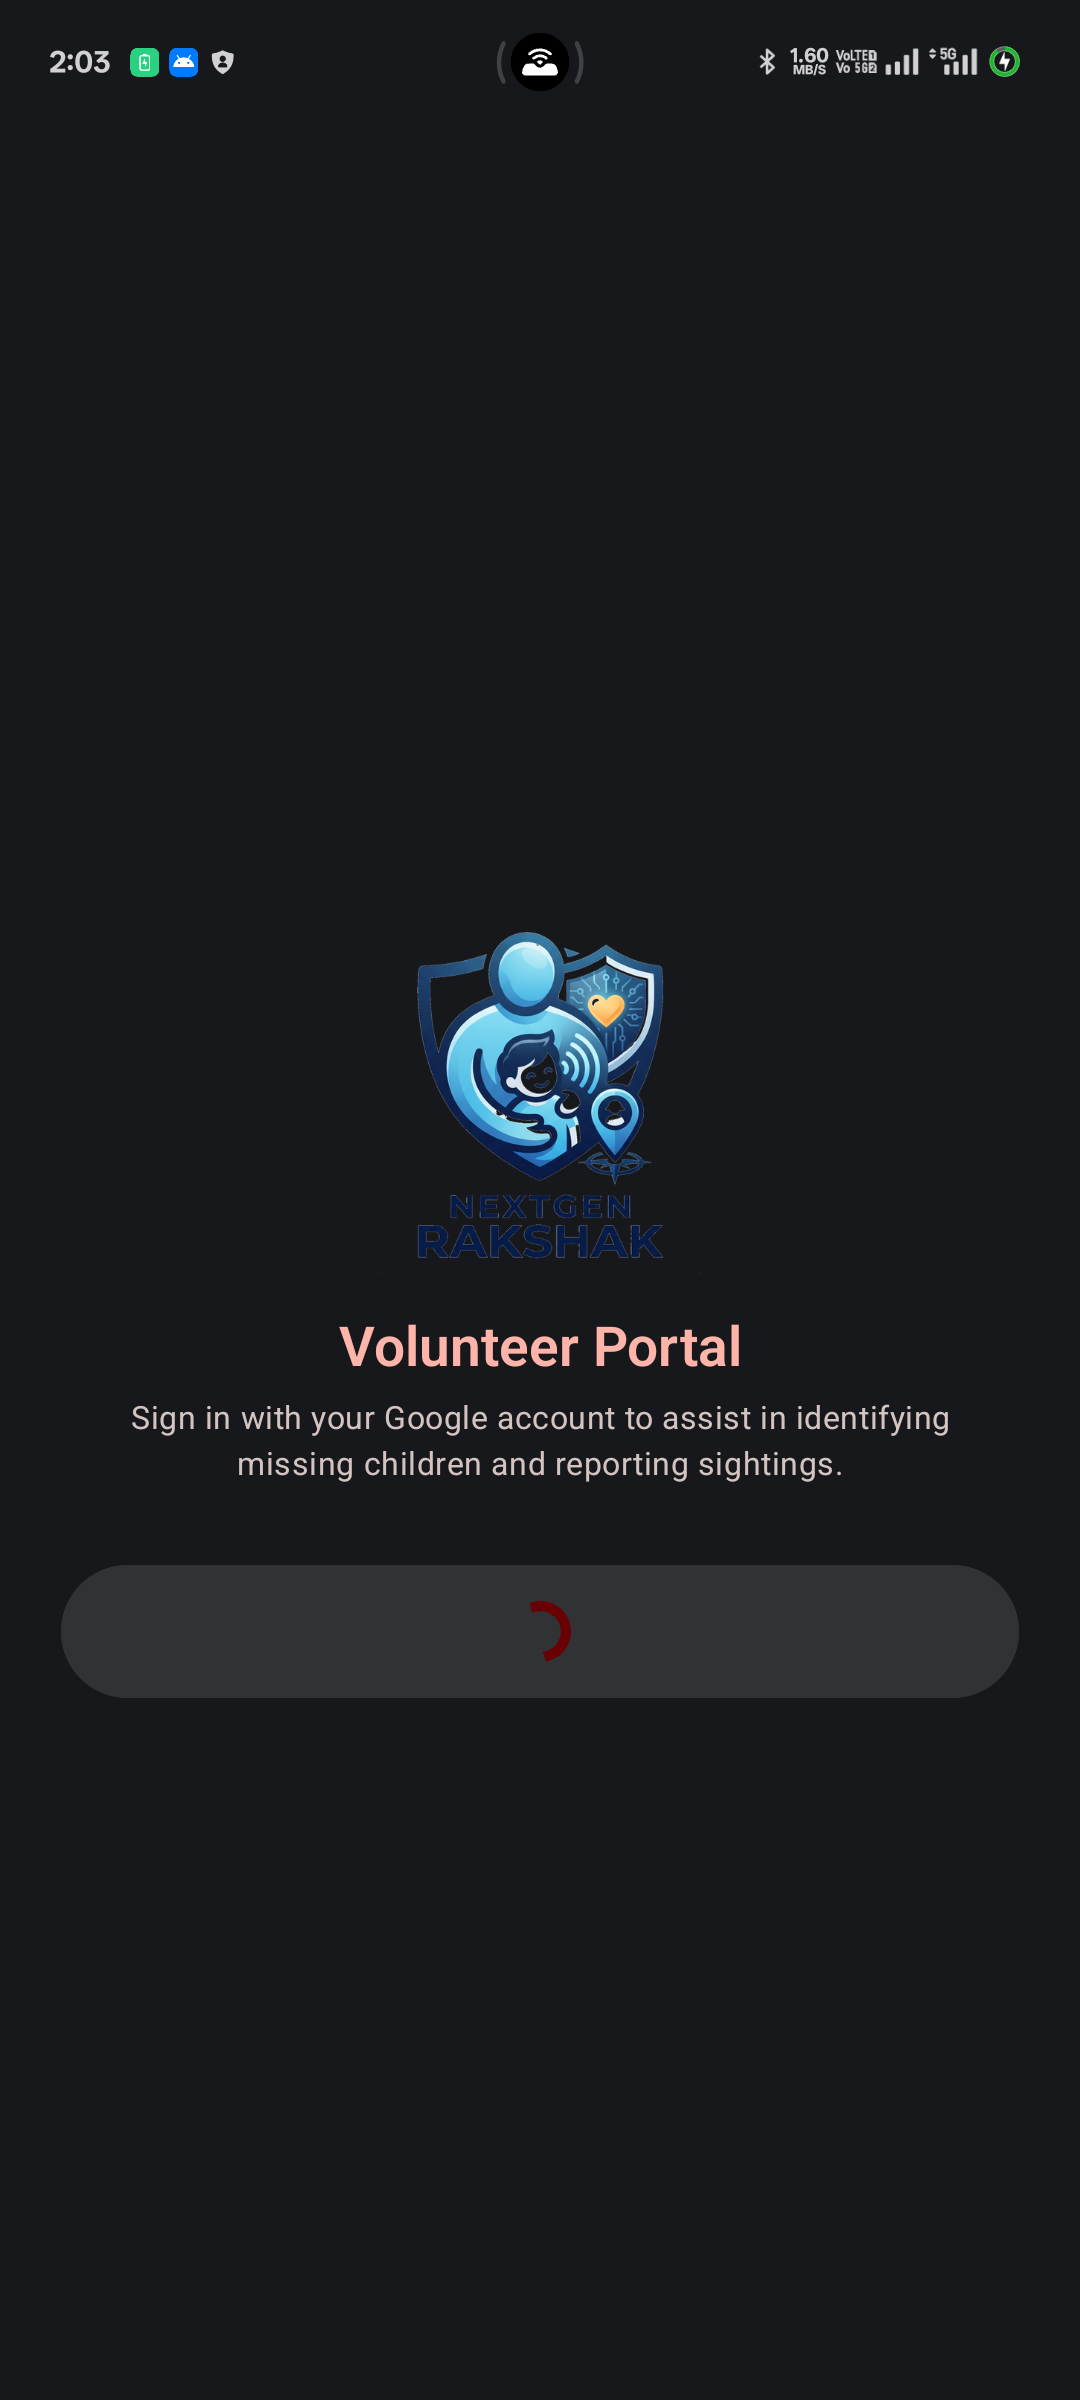
\includegraphics[width=\linewidth]{images/ss_03_signing_in.png}
  \caption{3. Signing in}
\end{subfigure}
\caption{Mobile workflow, screens 1--3: Google sign-in}
\label{fig:wf1}
\end{figure}

\begin{figure}[H]
\centering
\begin{subfigure}[t]{0.31\textwidth}
  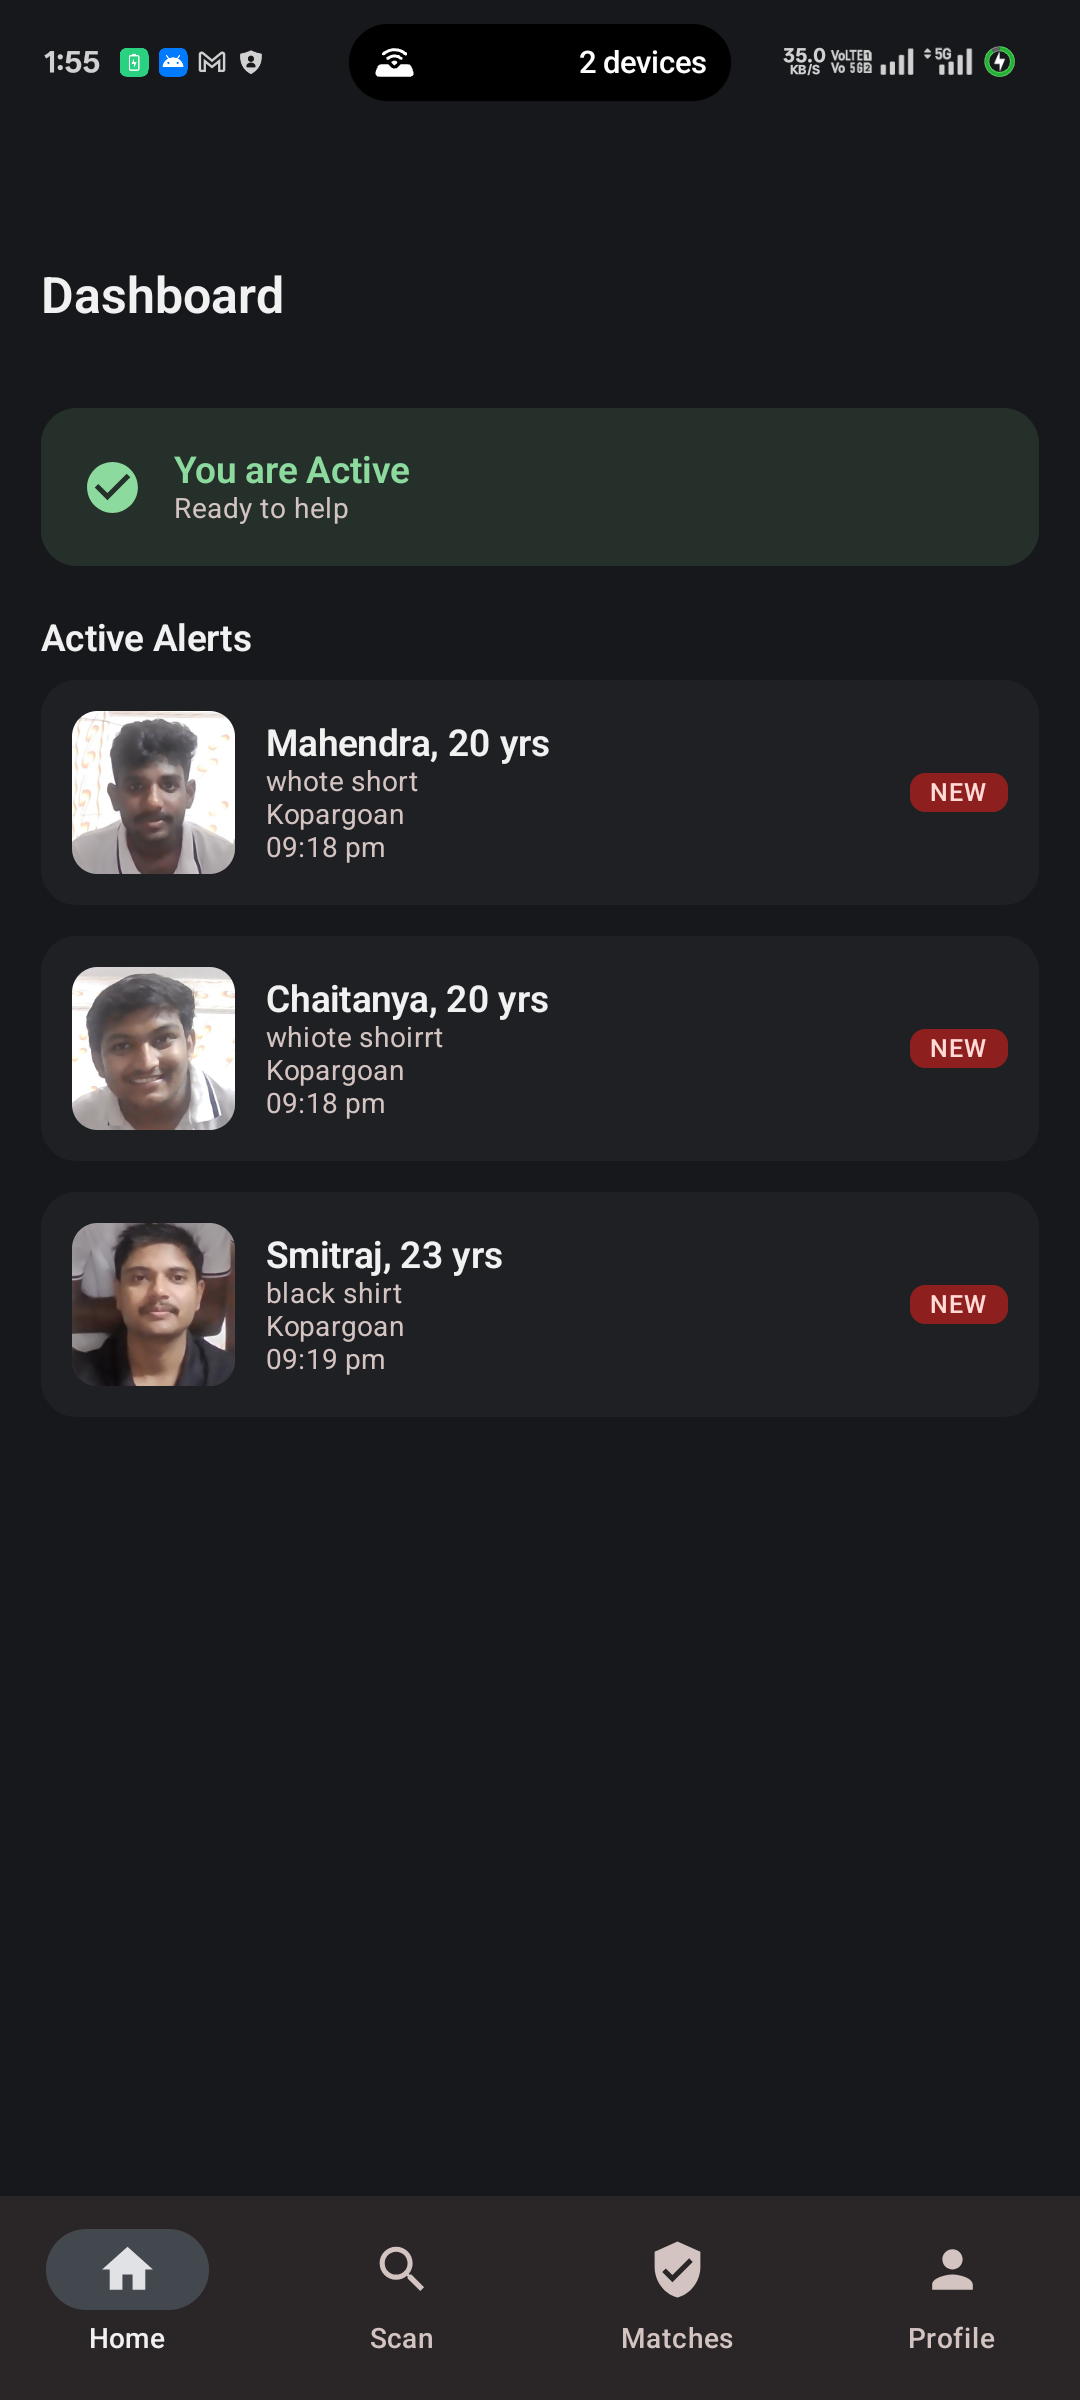
\includegraphics[width=\linewidth]{images/ss_04_home.png}
  \caption{4. Home dashboard}
\end{subfigure}\hfill
\begin{subfigure}[t]{0.31\textwidth}
  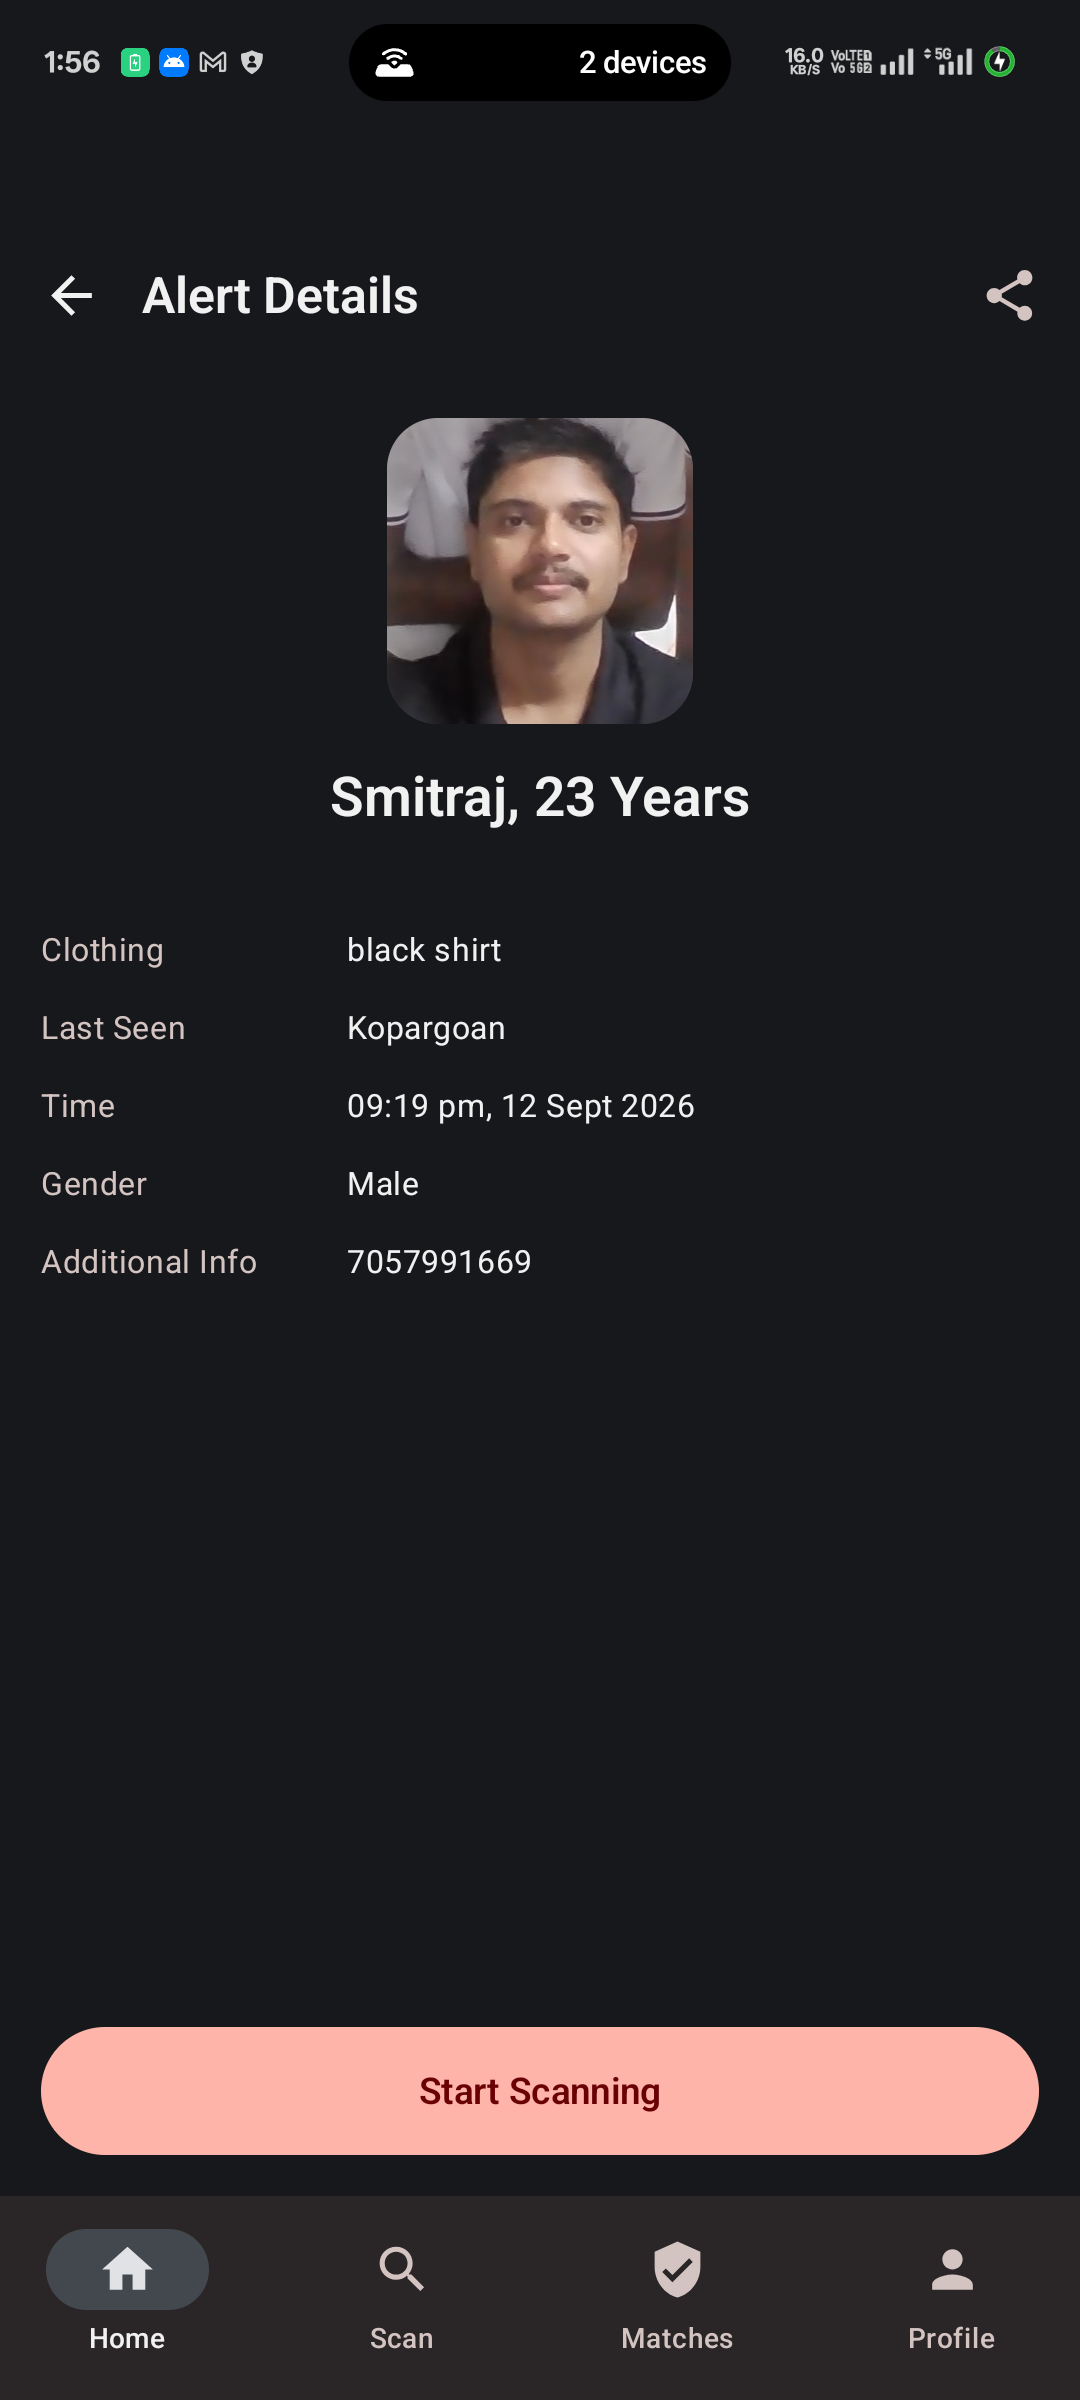
\includegraphics[width=\linewidth]{images/ss_05_alert_detail.png}
  \caption{5. Alert details}
\end{subfigure}\hfill
\begin{subfigure}[t]{0.31\textwidth}
  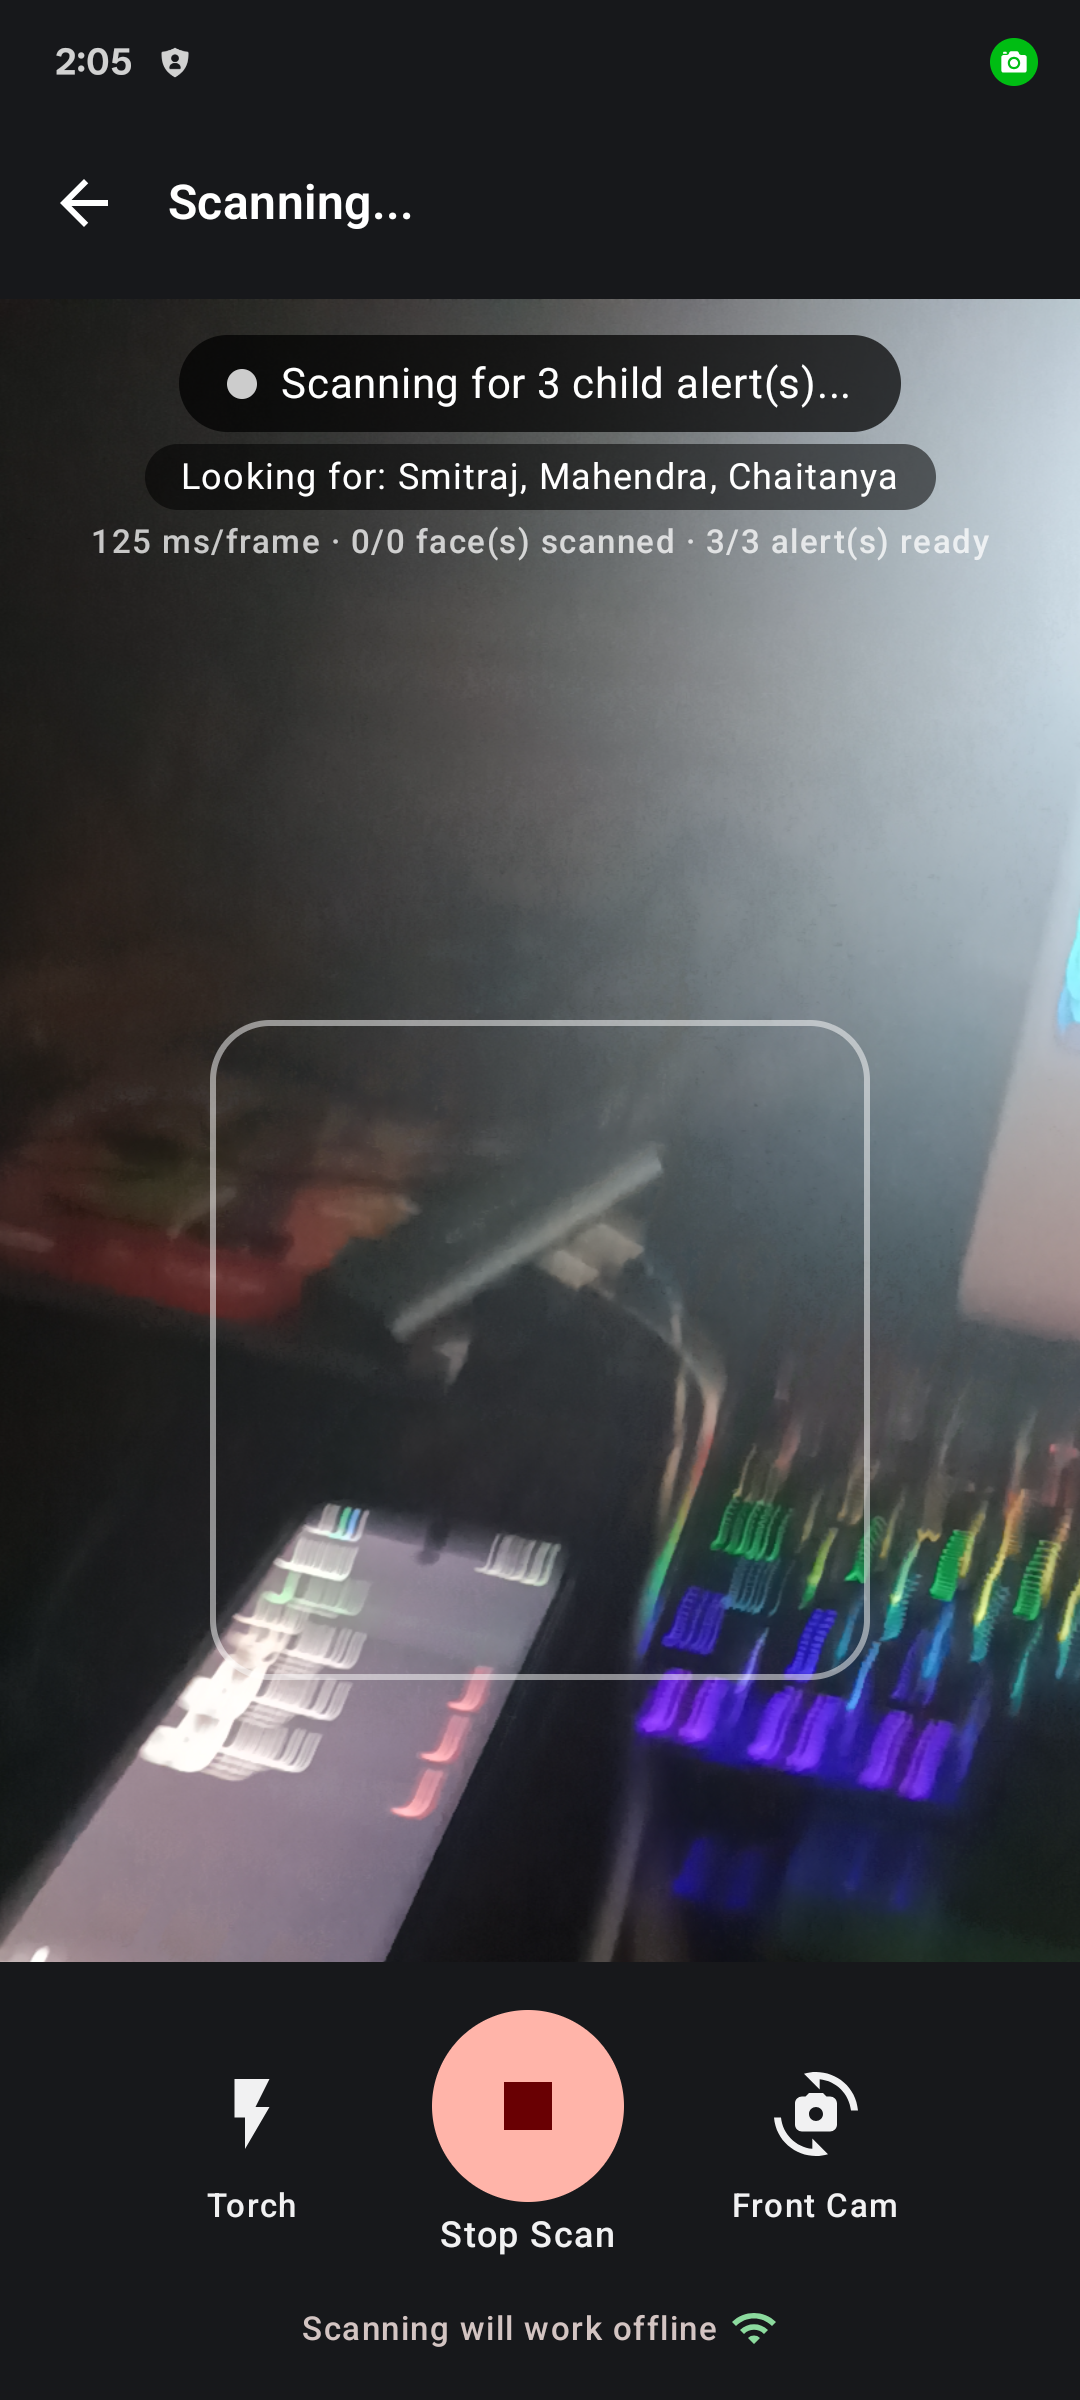
\includegraphics[width=\linewidth]{images/ss_06_scan.png}
  \caption{6. Live camera scan}
\end{subfigure}
\caption{Mobile workflow, screens 4--6: home, alert detail, and live scan}
\label{fig:wf2}
\end{figure}

\begin{figure}[H]
\centering
\begin{subfigure}[t]{0.31\textwidth}
  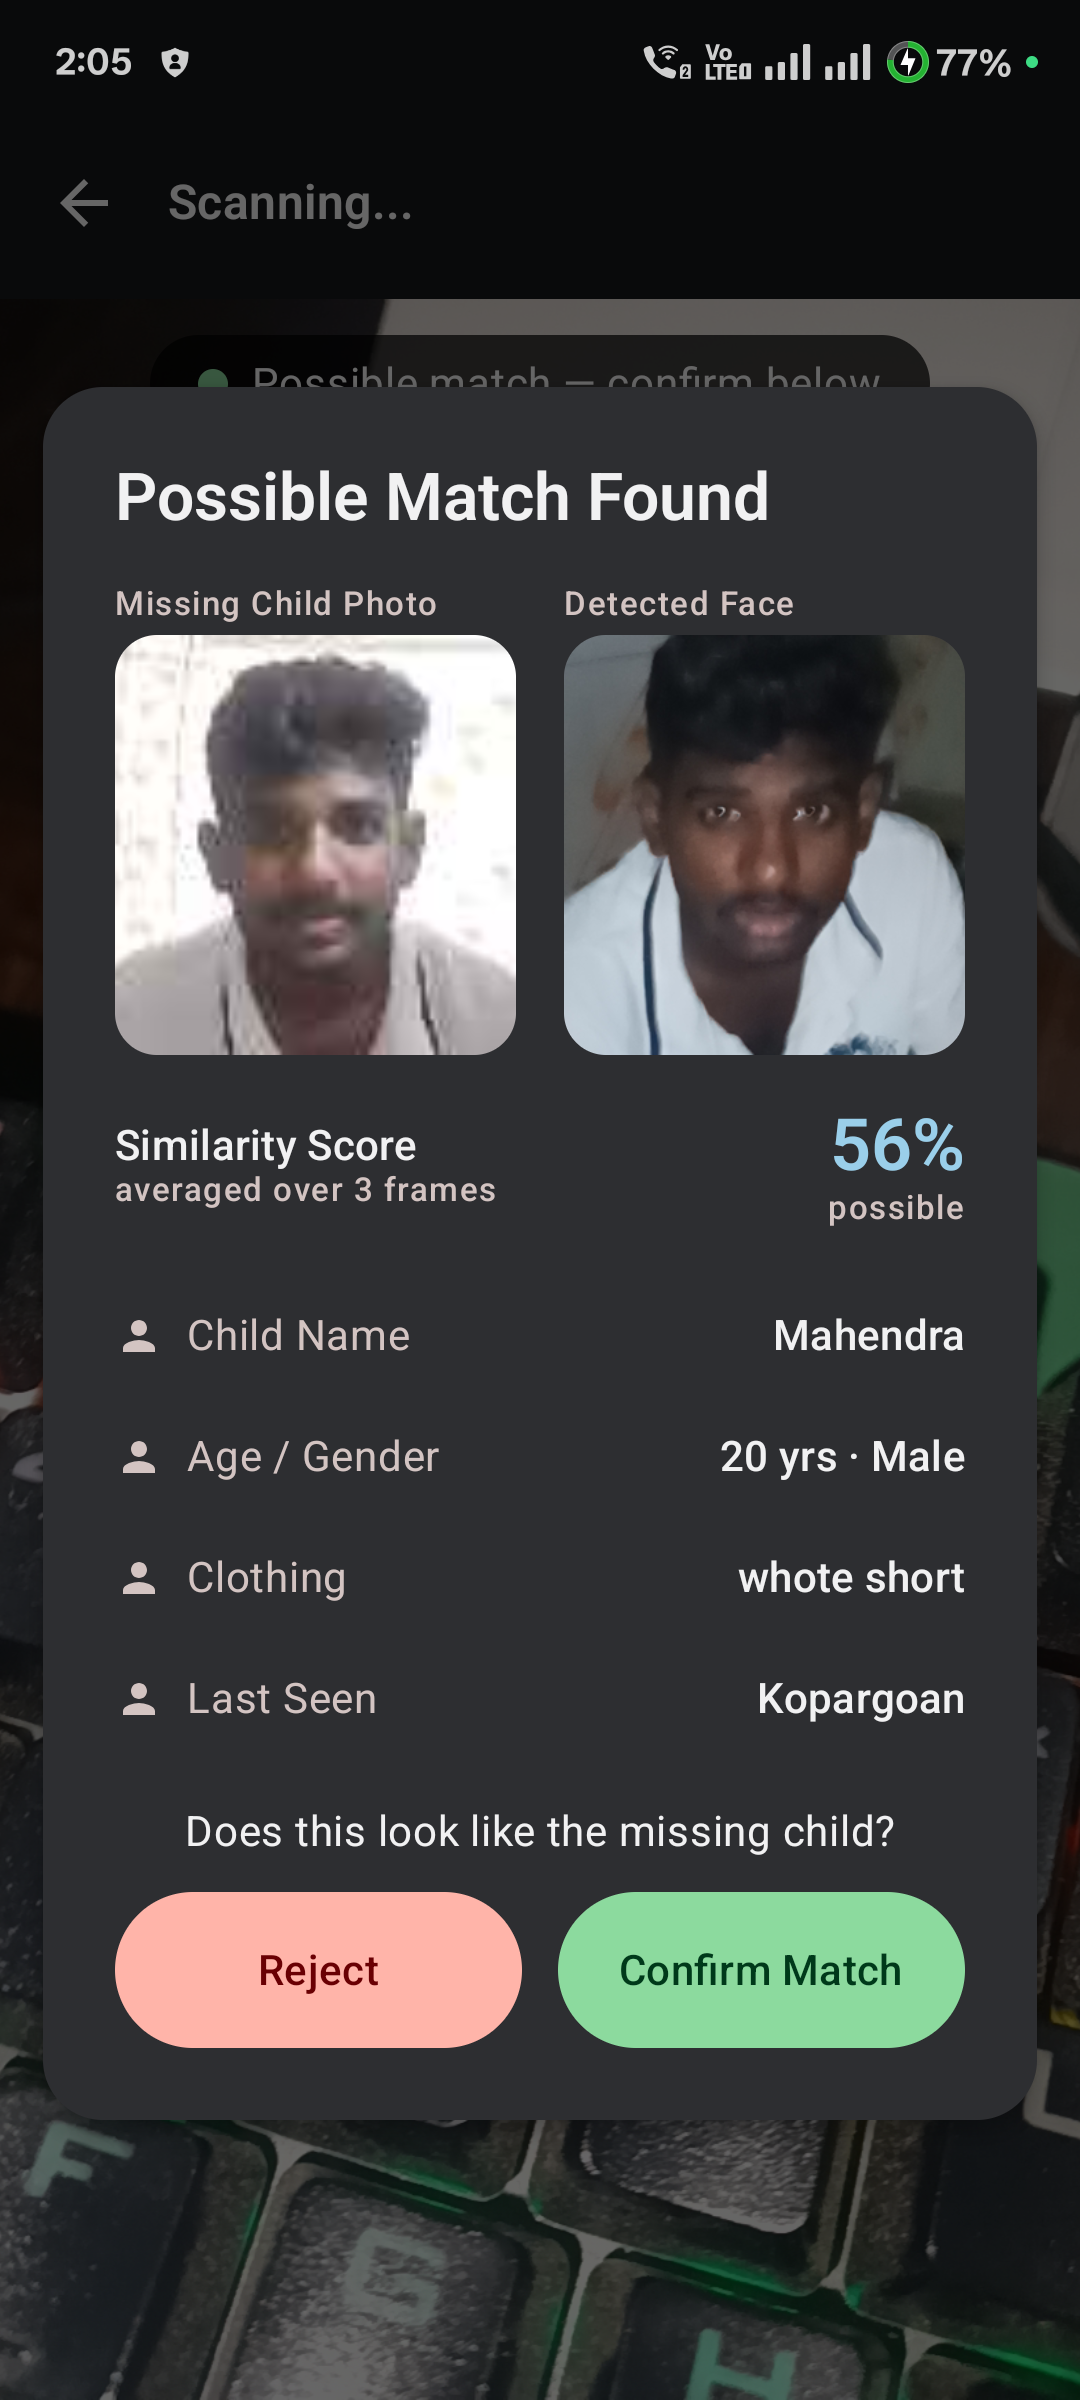
\includegraphics[width=\linewidth]{images/ss_07_match_popup.png}
  \caption{7. Possible-match popup}
\end{subfigure}\hfill
\begin{subfigure}[t]{0.31\textwidth}
  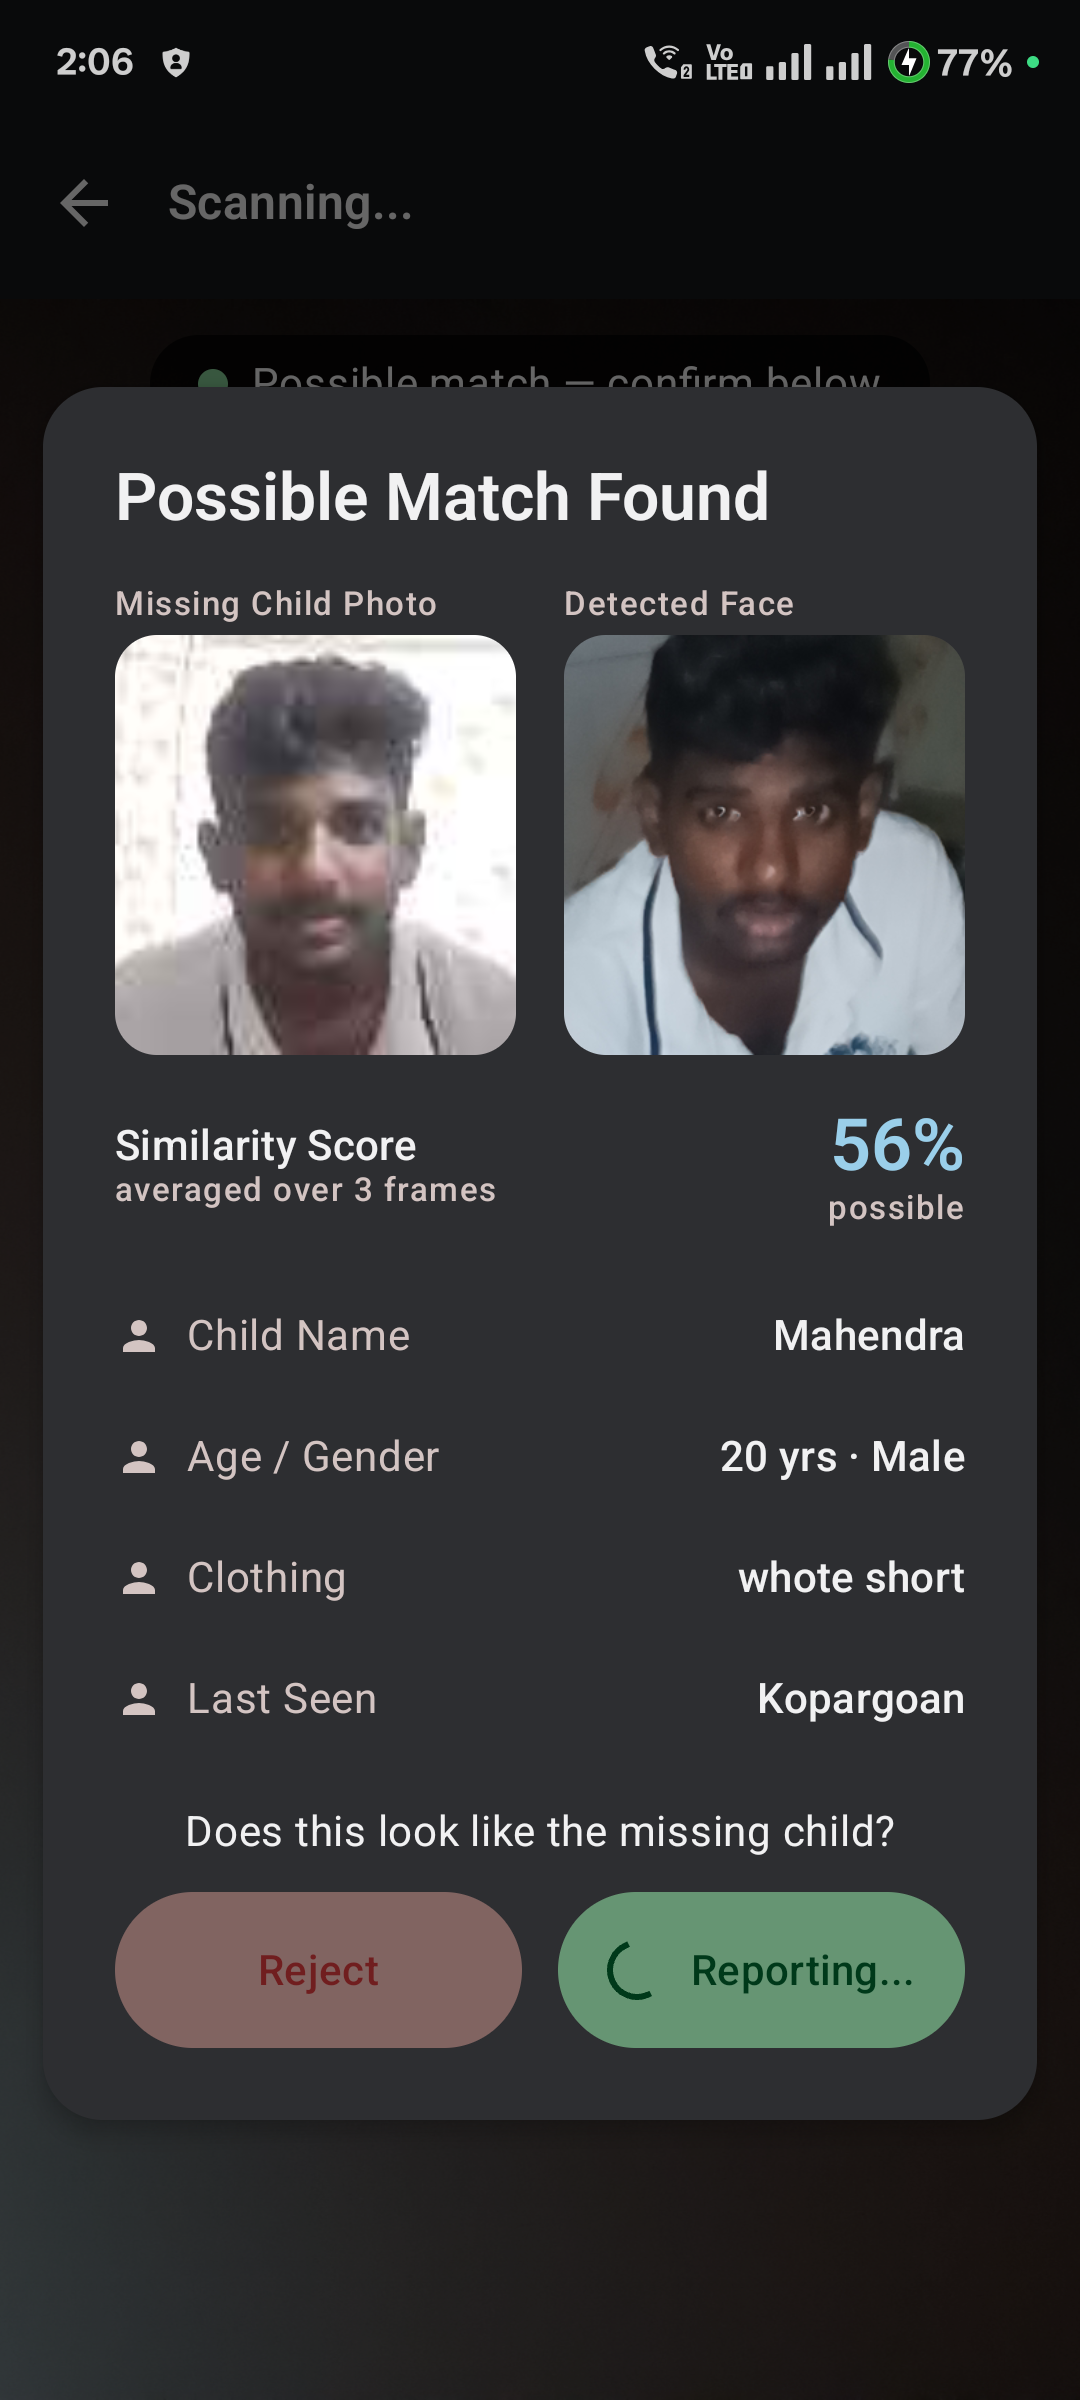
\includegraphics[width=\linewidth]{images/ss_08_confirming.png}
  \caption{8. Confirming the match}
\end{subfigure}\hfill
\begin{subfigure}[t]{0.31\textwidth}
  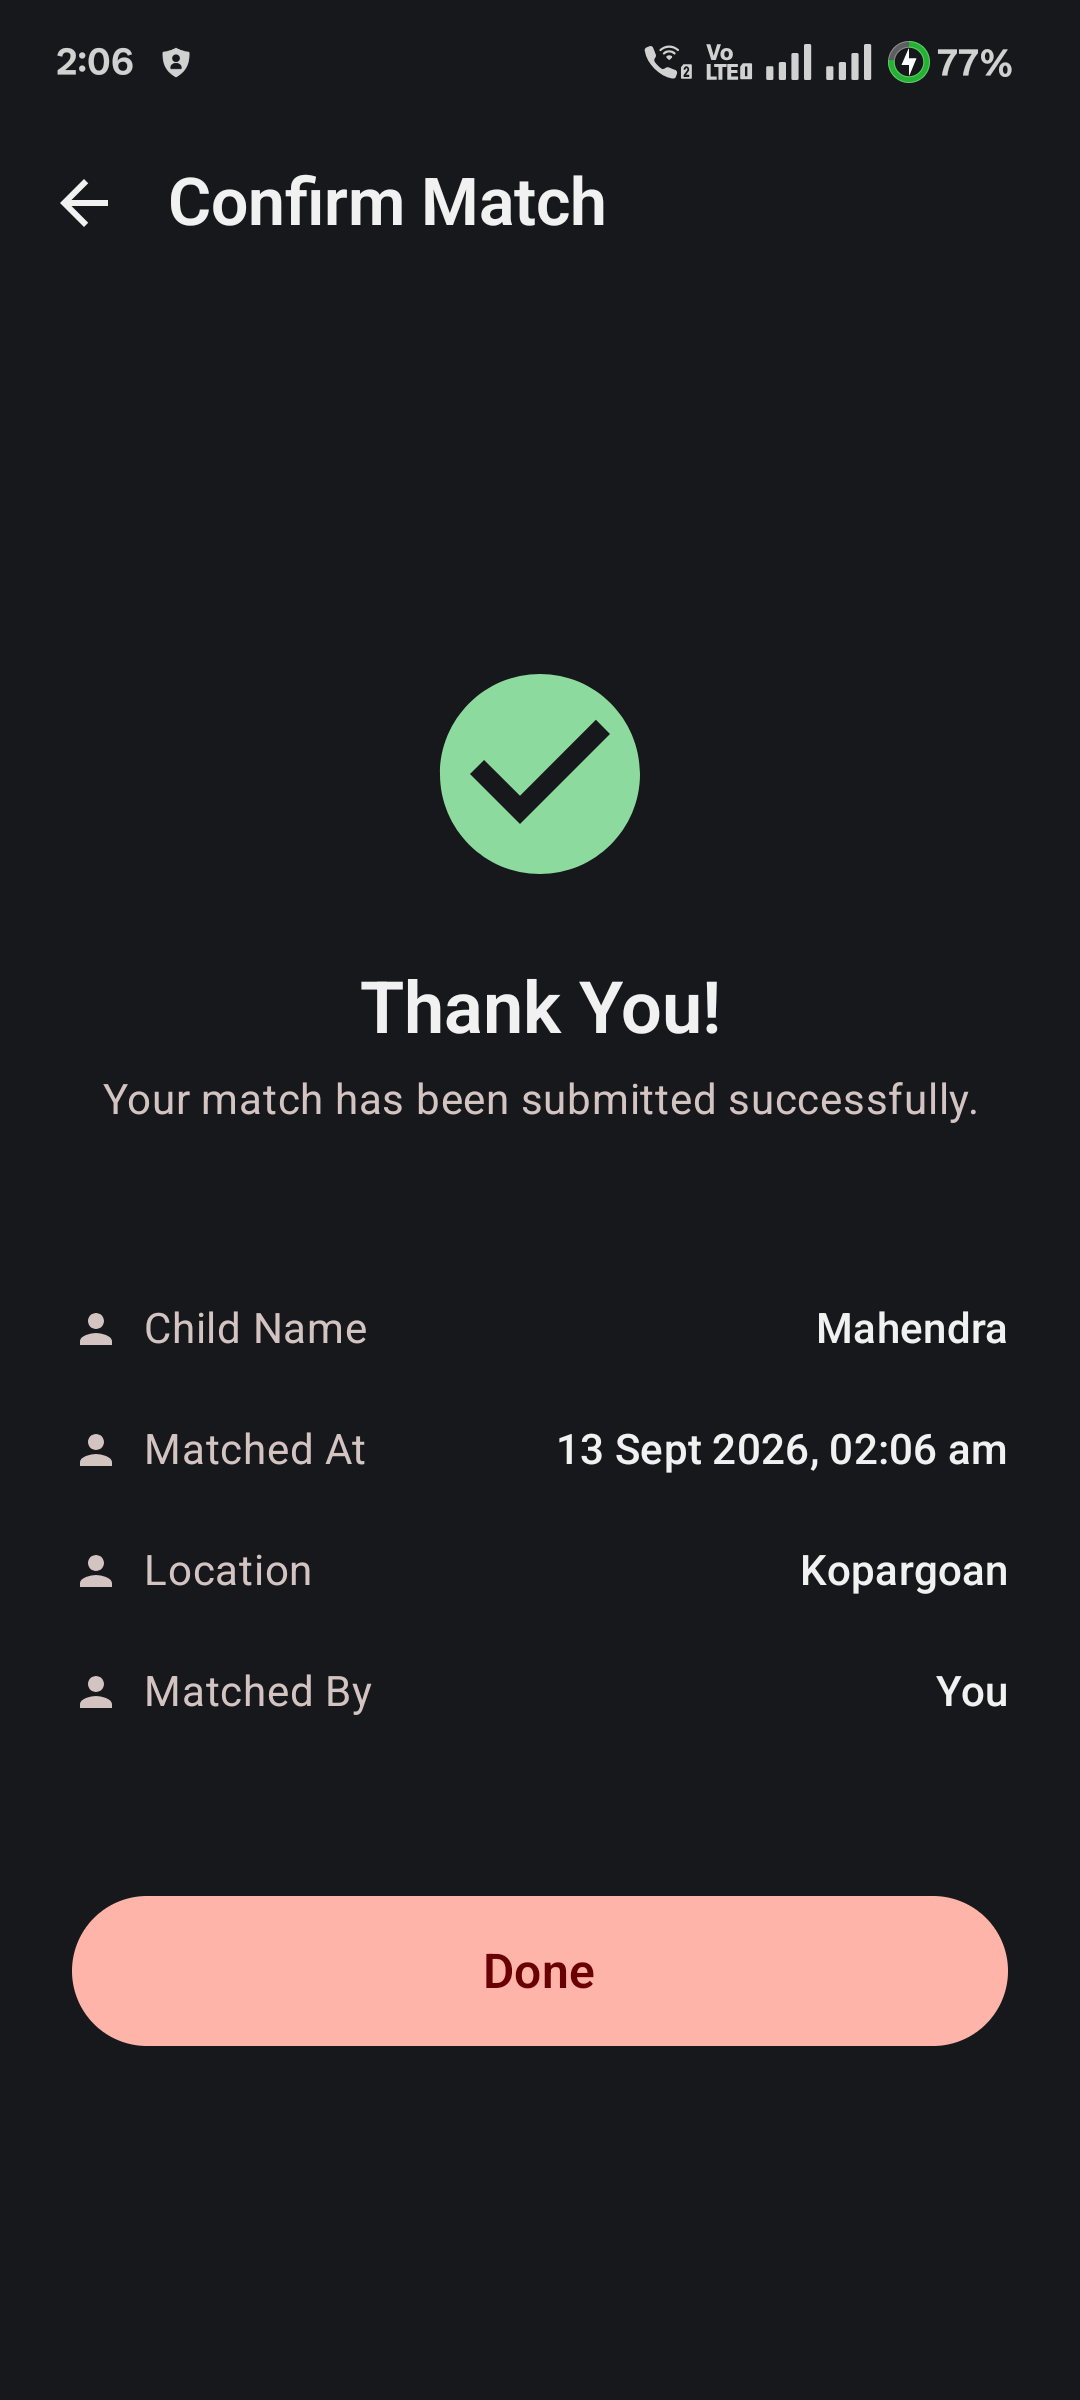
\includegraphics[width=\linewidth]{images/ss_09_thankyou.png}
  \caption{9. Match submitted}
\end{subfigure}
\caption{Mobile workflow, screens 7--9: candidate match through confirmation}
\label{fig:wf3}
\end{figure}

\begin{figure}[H]
\centering
\begin{subfigure}[t]{0.31\textwidth}
  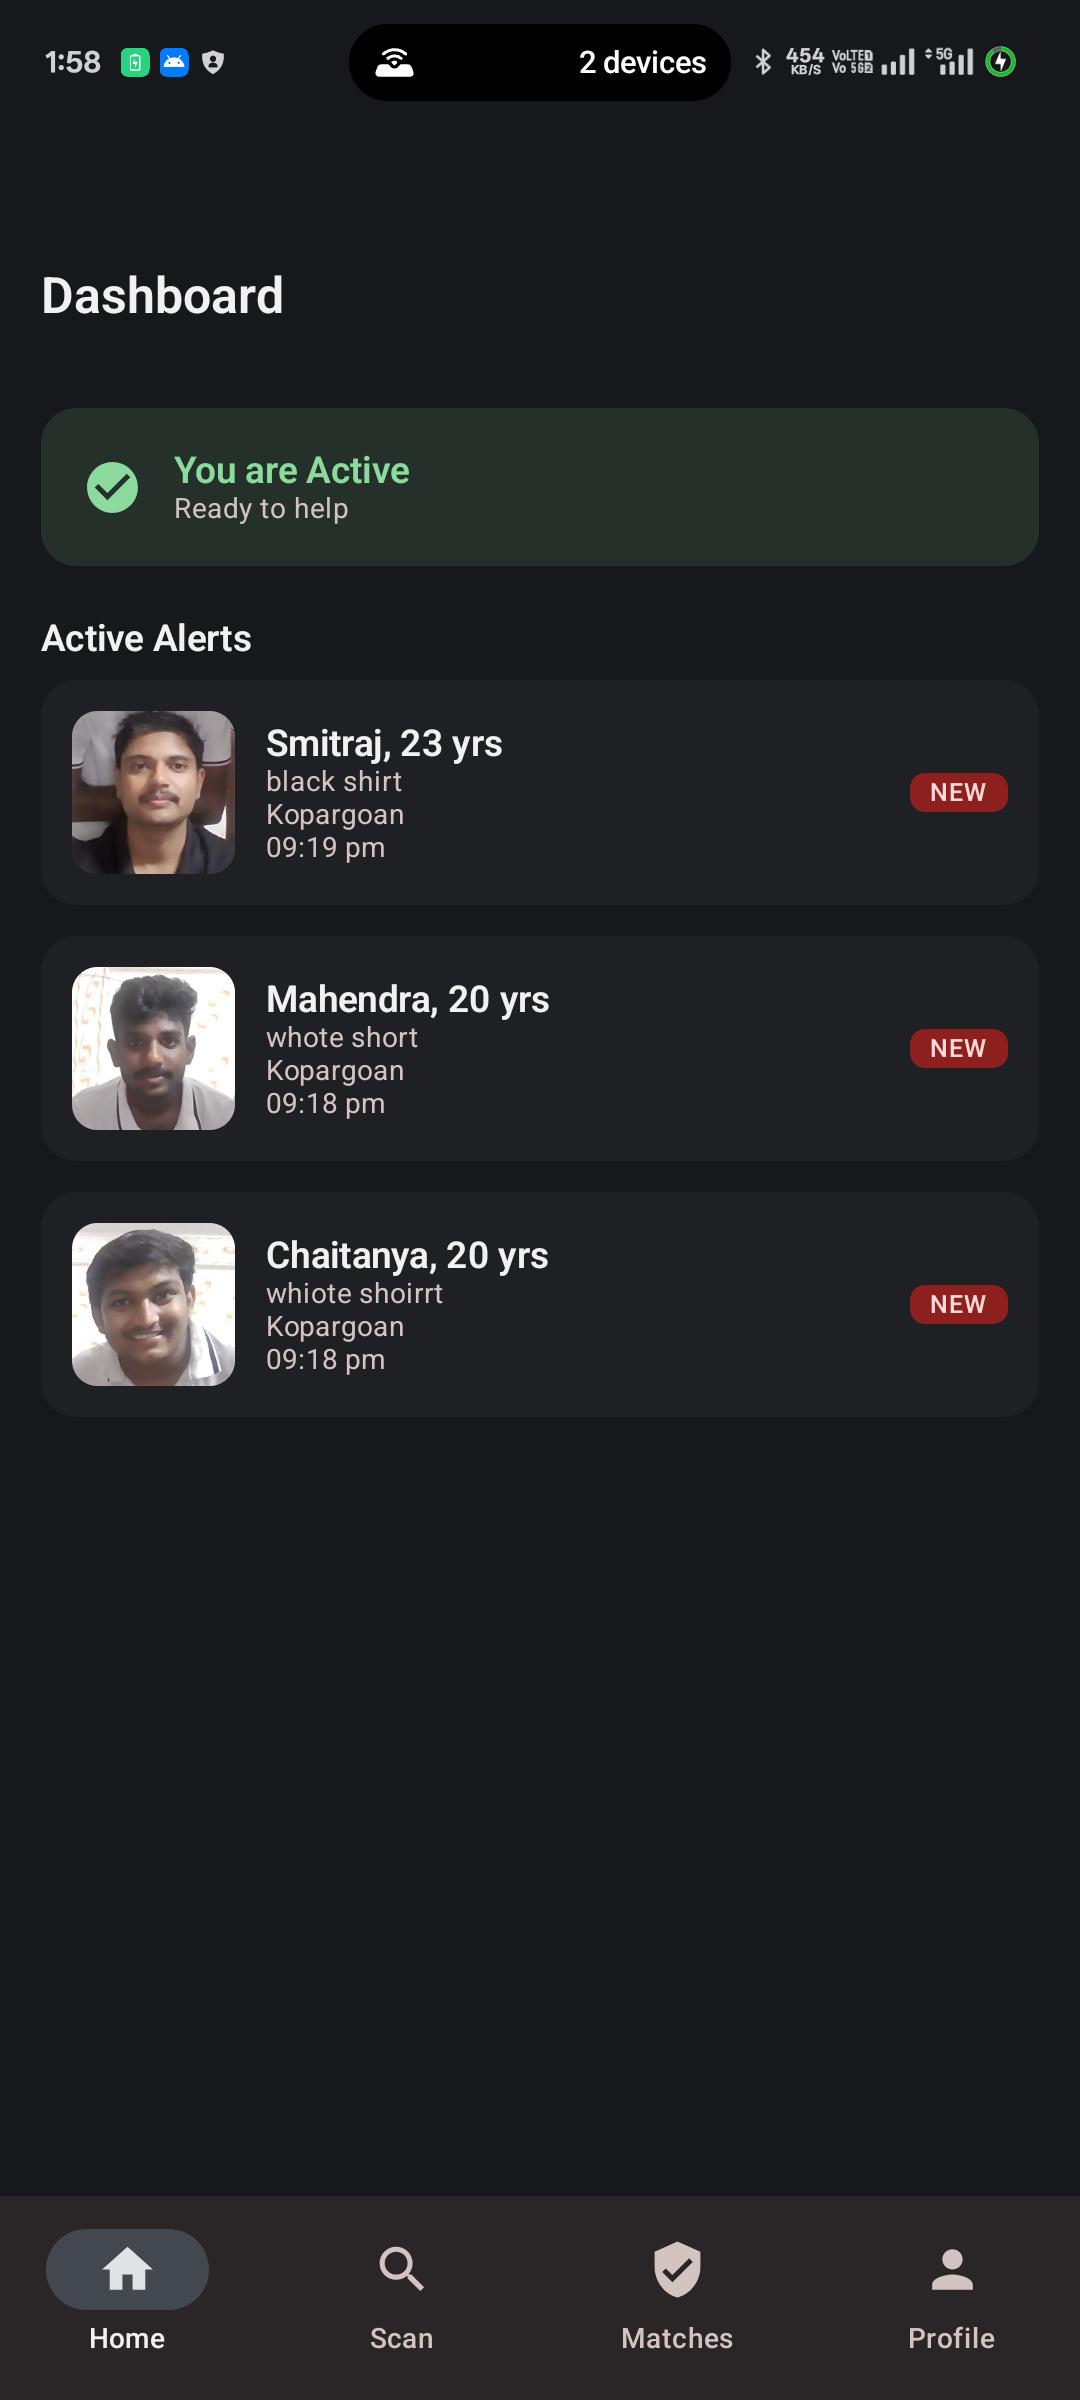
\includegraphics[width=\linewidth]{images/ss_10_home_after_match.png}
  \caption{10. Home after match}
\end{subfigure}\hfill
\begin{subfigure}[t]{0.31\textwidth}
  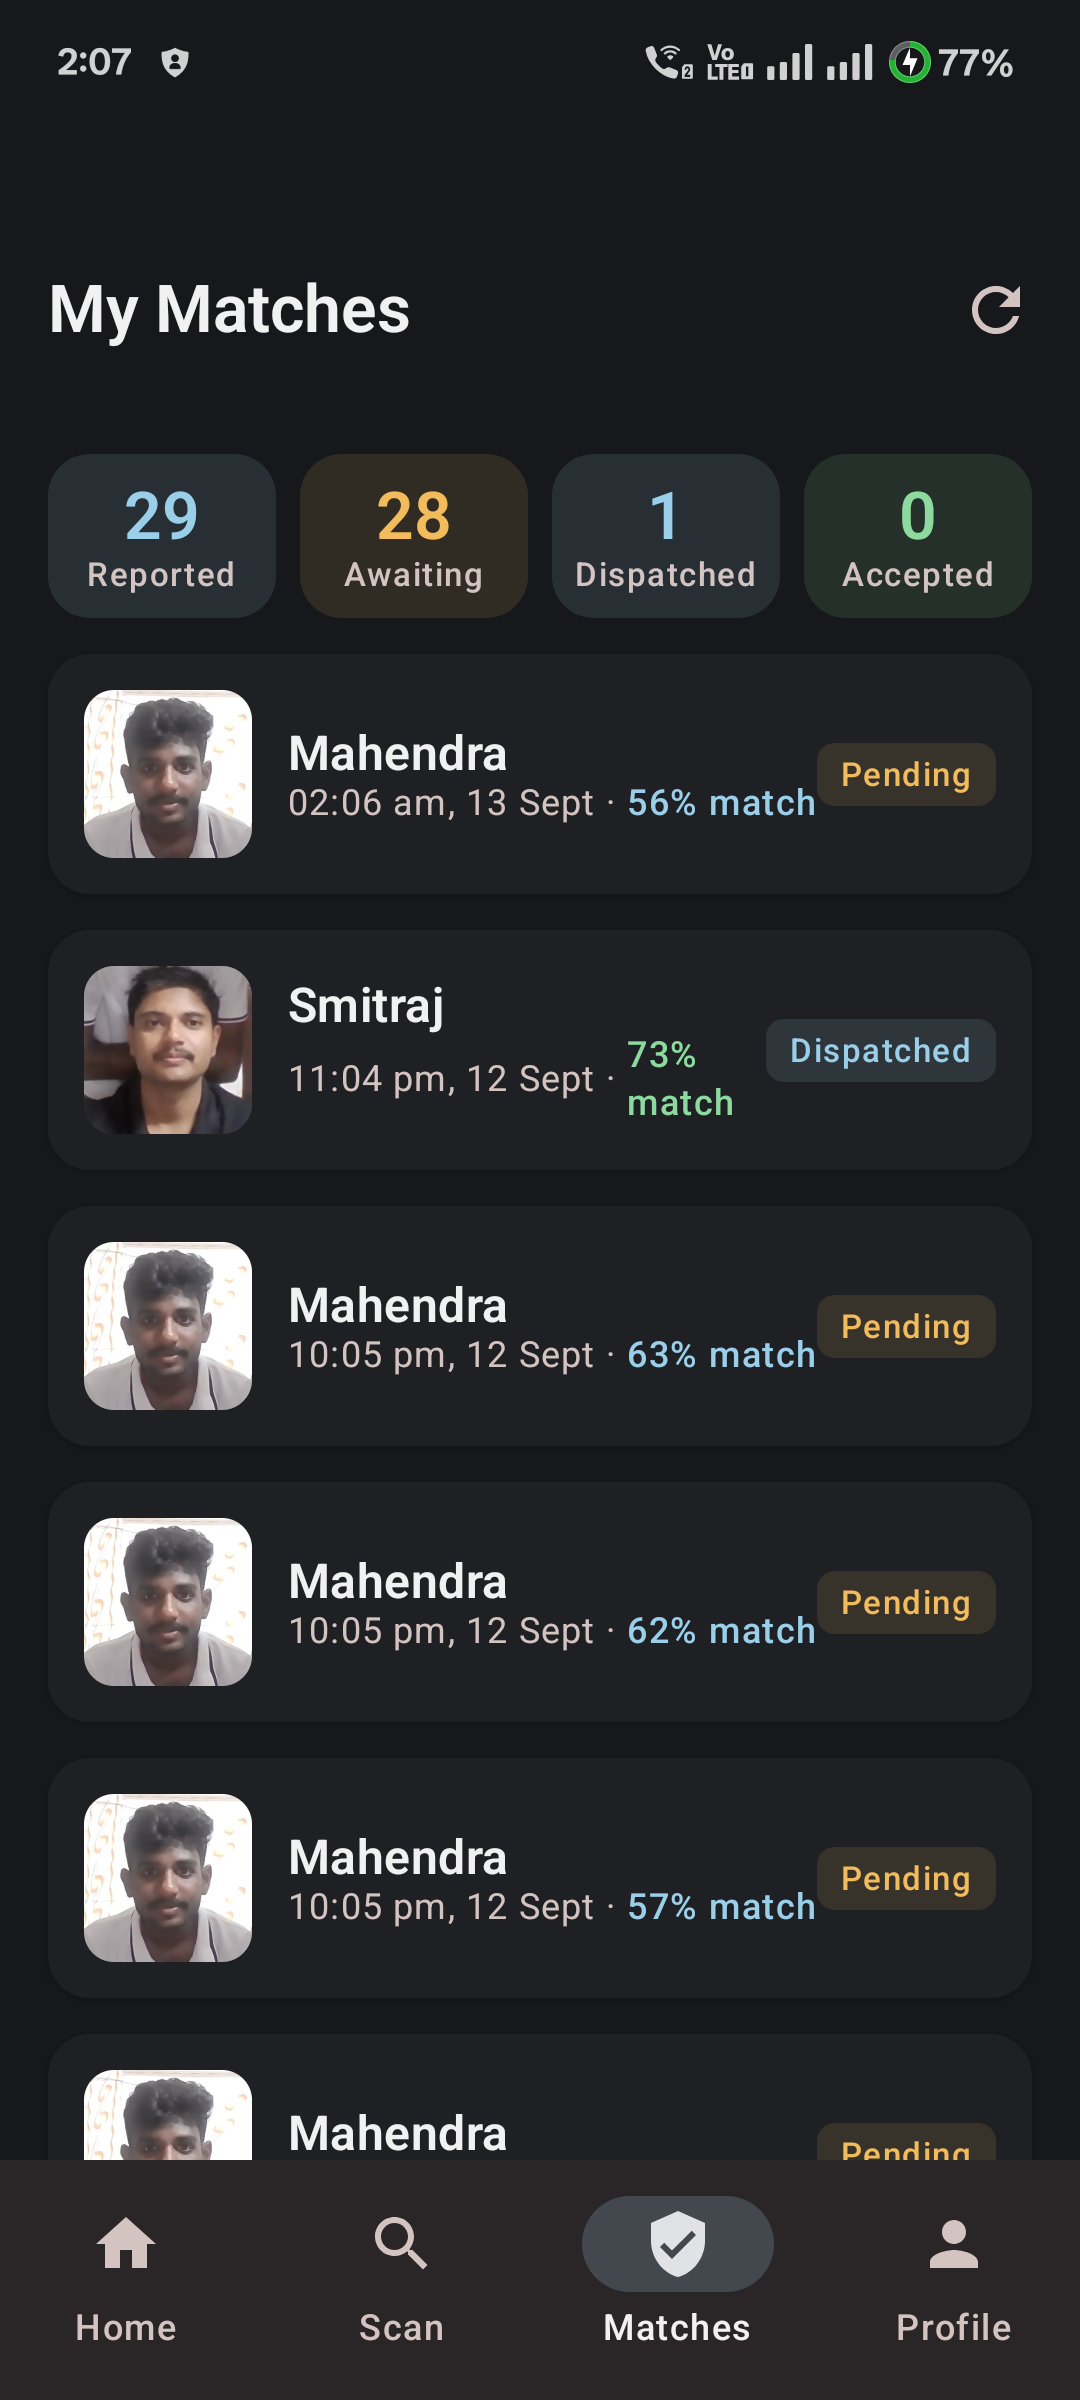
\includegraphics[width=\linewidth]{images/ss_11_matches.png}
  \caption{11. Matches list}
\end{subfigure}\hfill
\begin{subfigure}[t]{0.31\textwidth}
  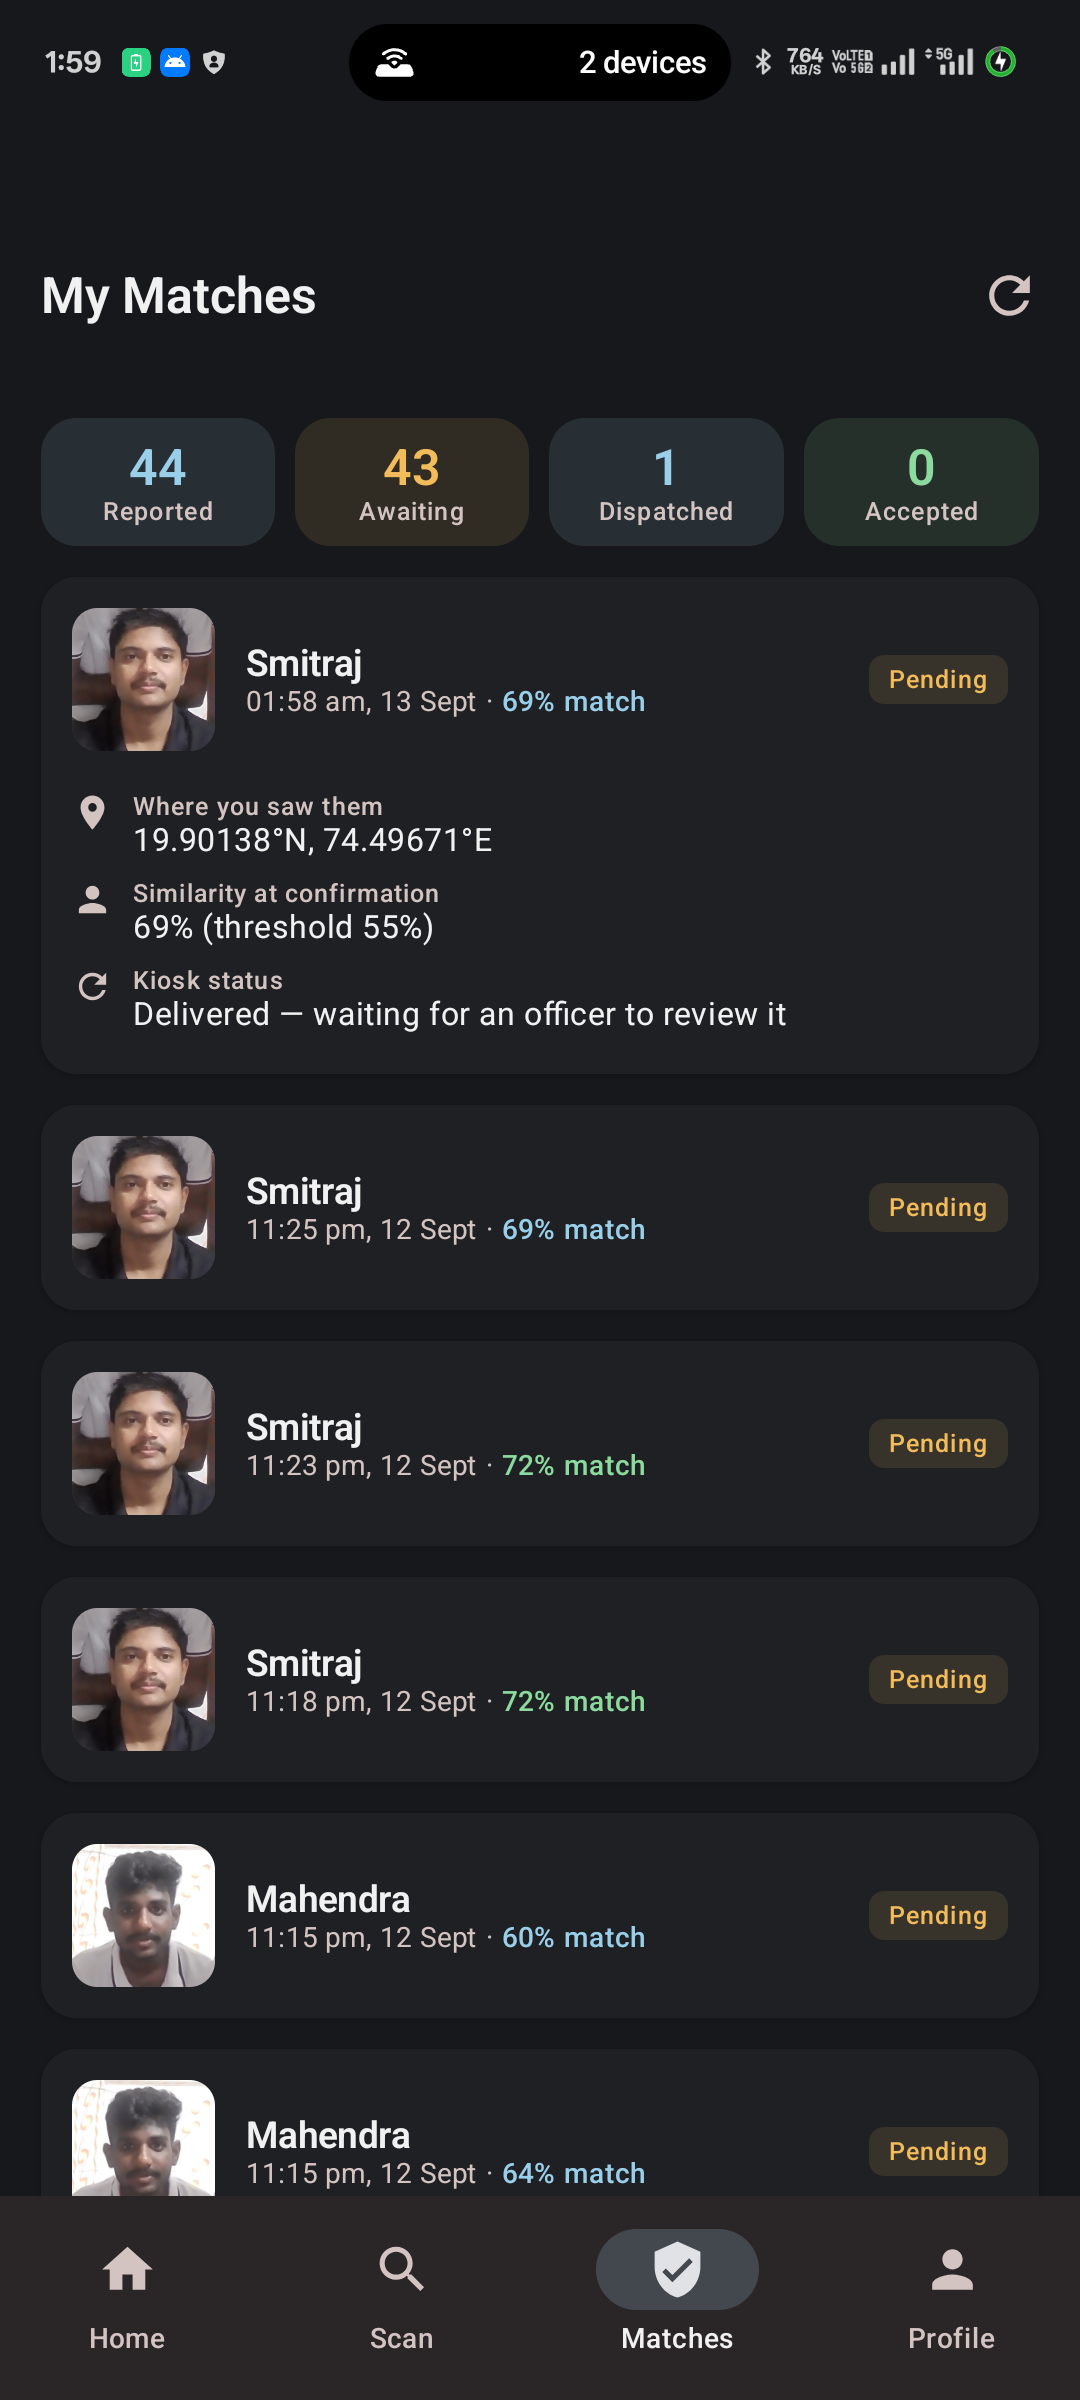
\includegraphics[width=\linewidth]{images/ss_12_match_detail.png}
  \caption{12. Match -- expanded detail}
\end{subfigure}
\caption{Mobile workflow, screens 10--12: post-match home and match history}
\label{fig:wf4}
\end{figure}

\begin{figure}[H]
\centering
\begin{subfigure}[t]{0.31\textwidth}
  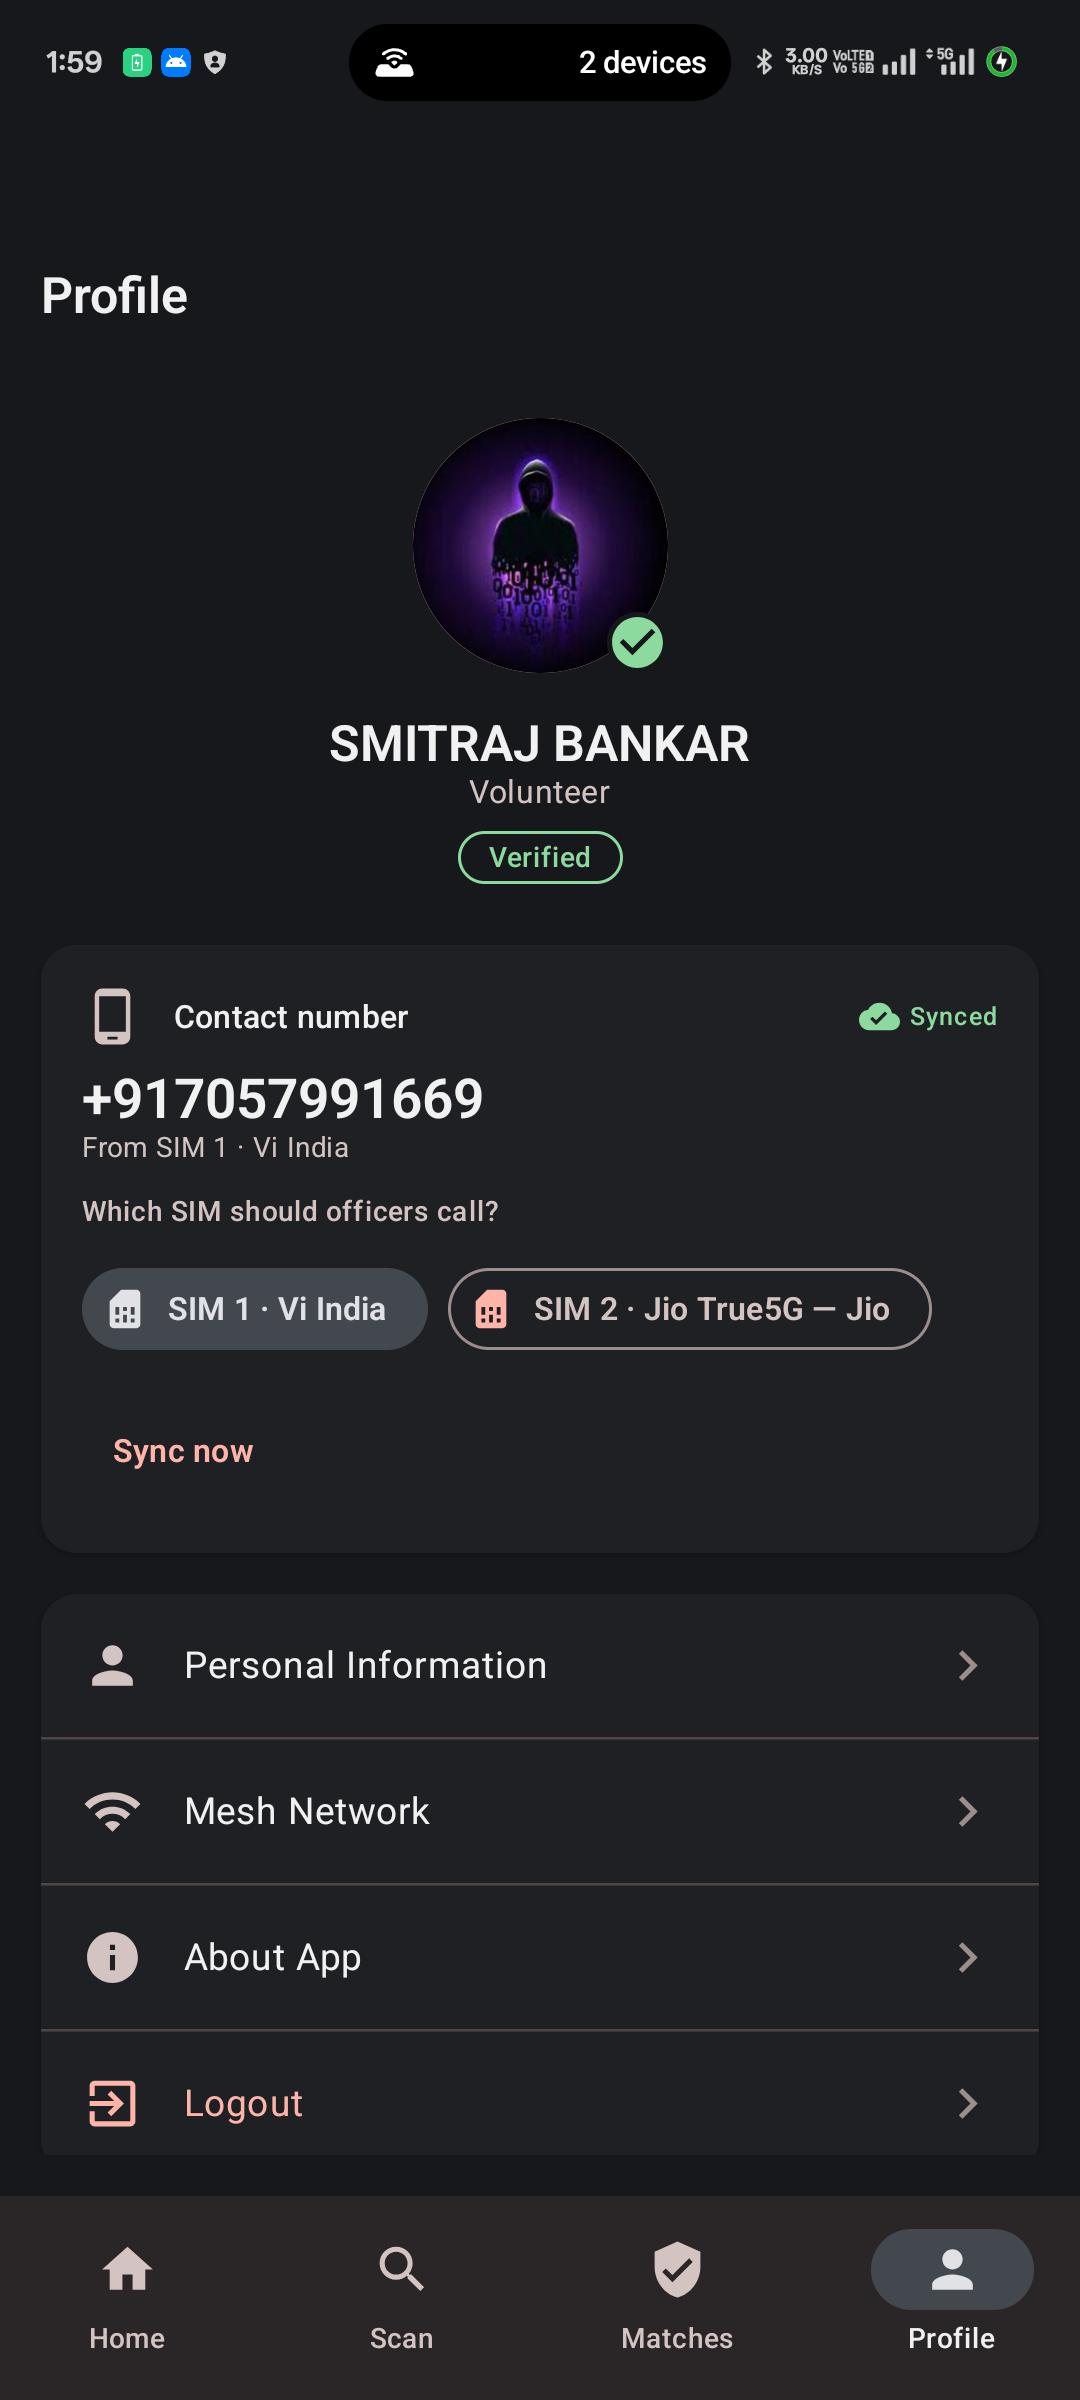
\includegraphics[width=\linewidth]{images/ss_13_profile.png}
  \caption{13. Profile}
\end{subfigure}\hfill
\begin{subfigure}[t]{0.31\textwidth}
  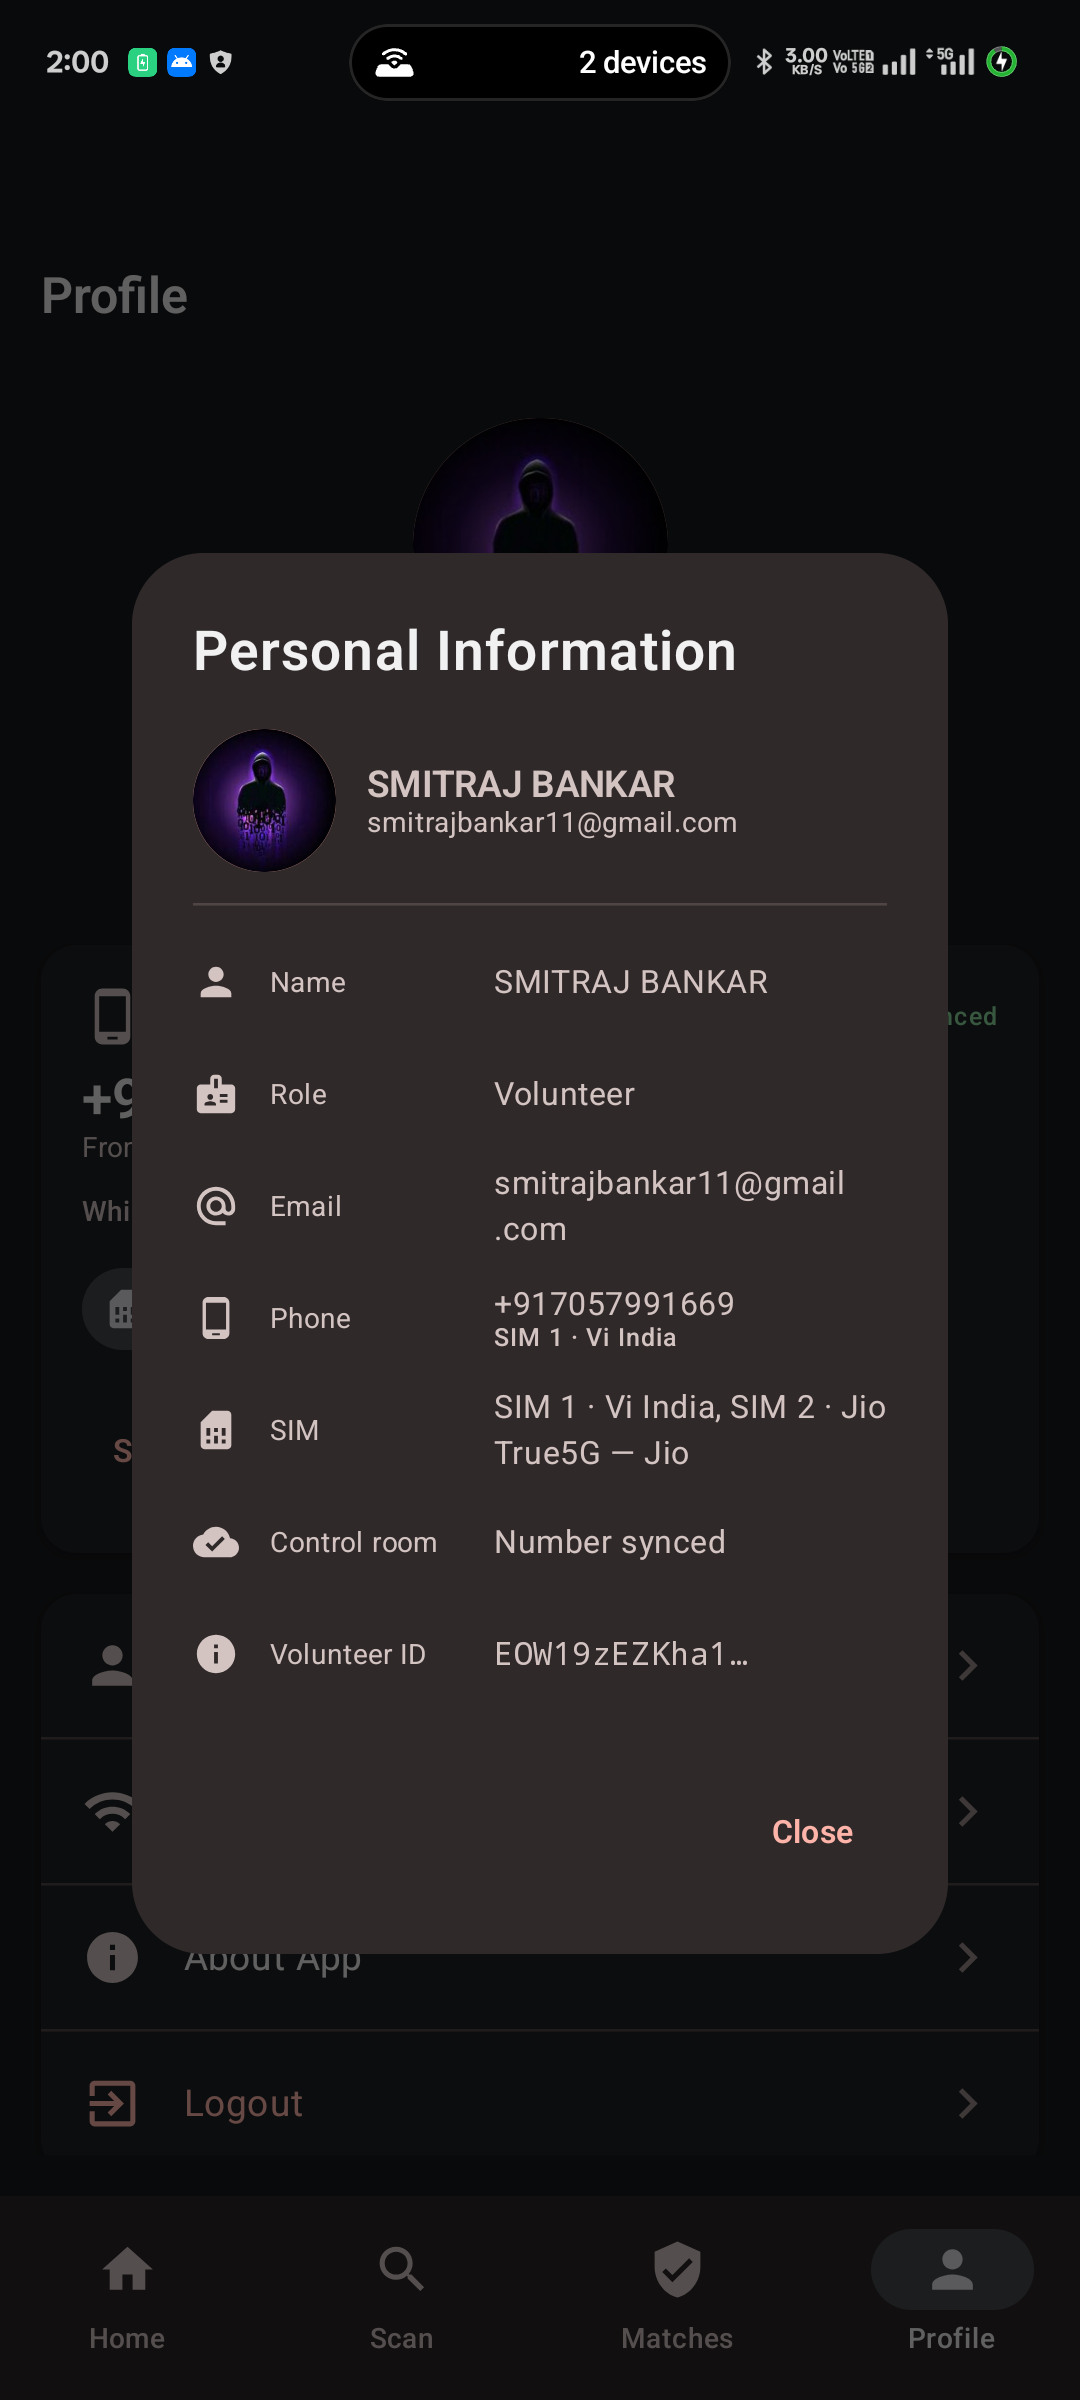
\includegraphics[width=\linewidth]{images/ss_14_personal_info.png}
  \caption{14. Personal info}
\end{subfigure}\hfill
\begin{subfigure}[t]{0.31\textwidth}
  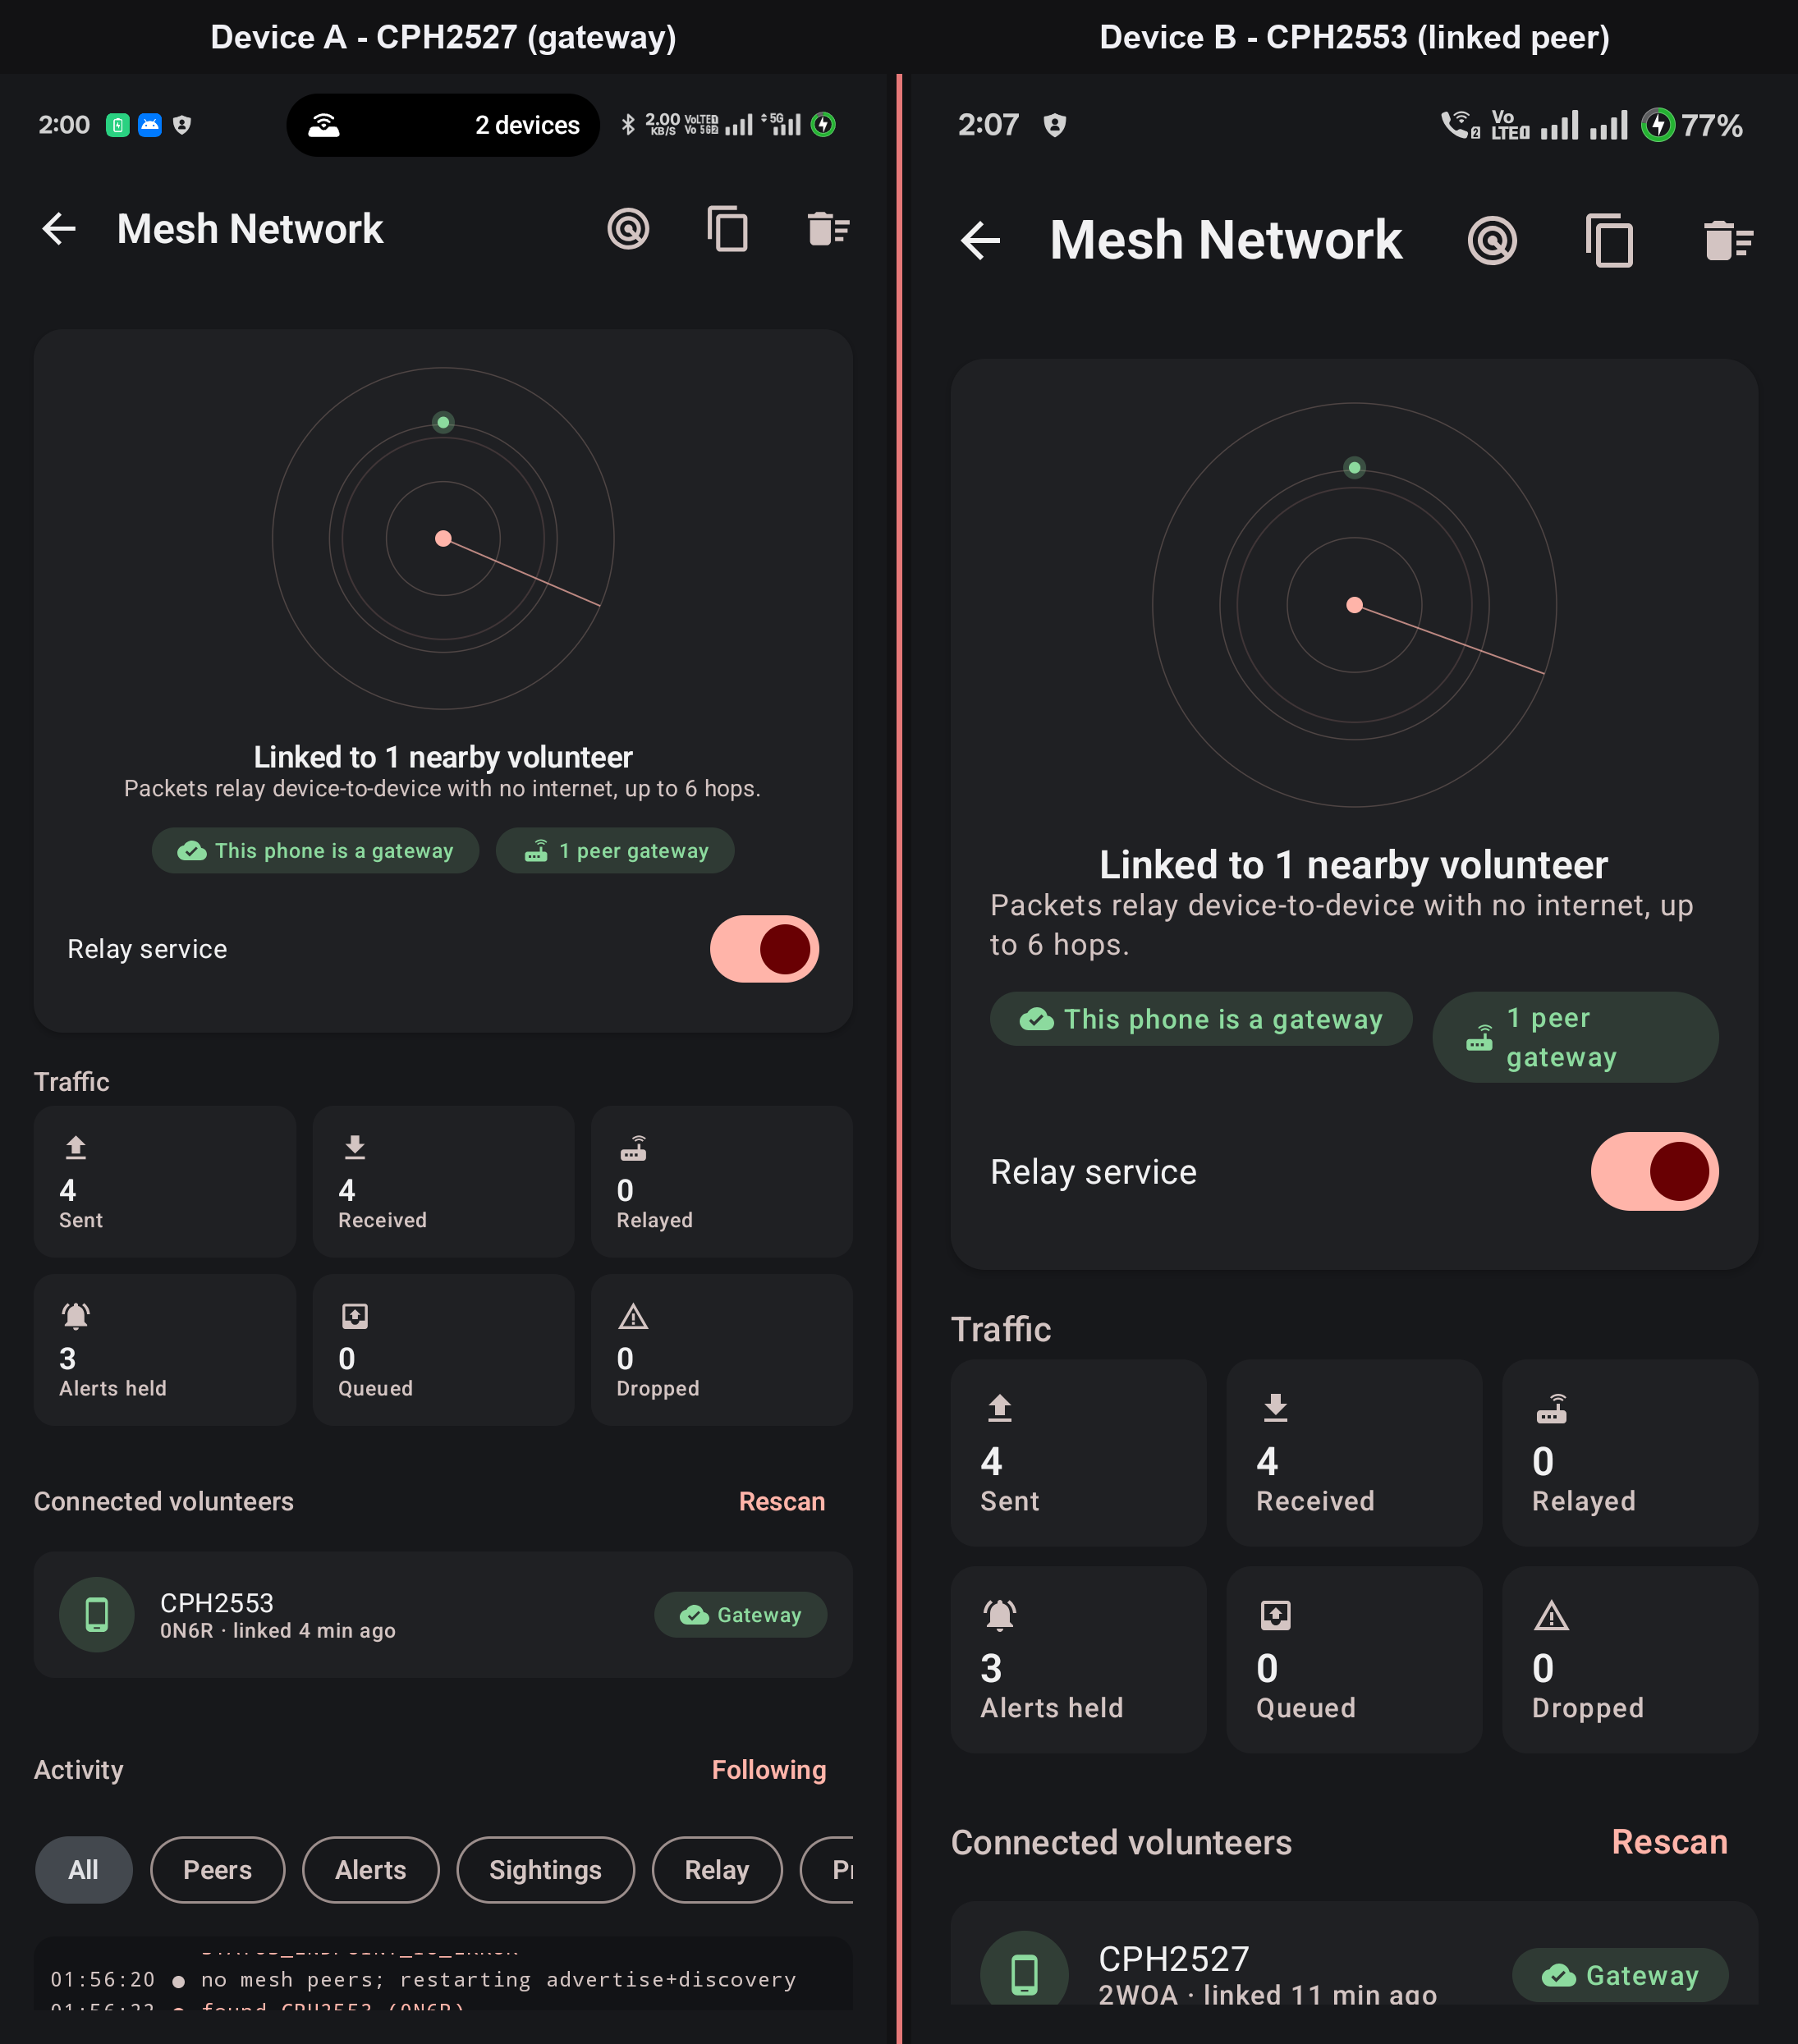
\includegraphics[width=\linewidth]{images/ss_15_mesh_compare.png}
  \caption{15. Mesh network view}
\end{subfigure}
\caption{Mobile workflow, screens 13--15: profile, personal info, and mesh screen}
\label{fig:wf5}
\end{figure}

\begin{figure}[H]
\centering
\begin{subfigure}[t]{0.31\textwidth}
  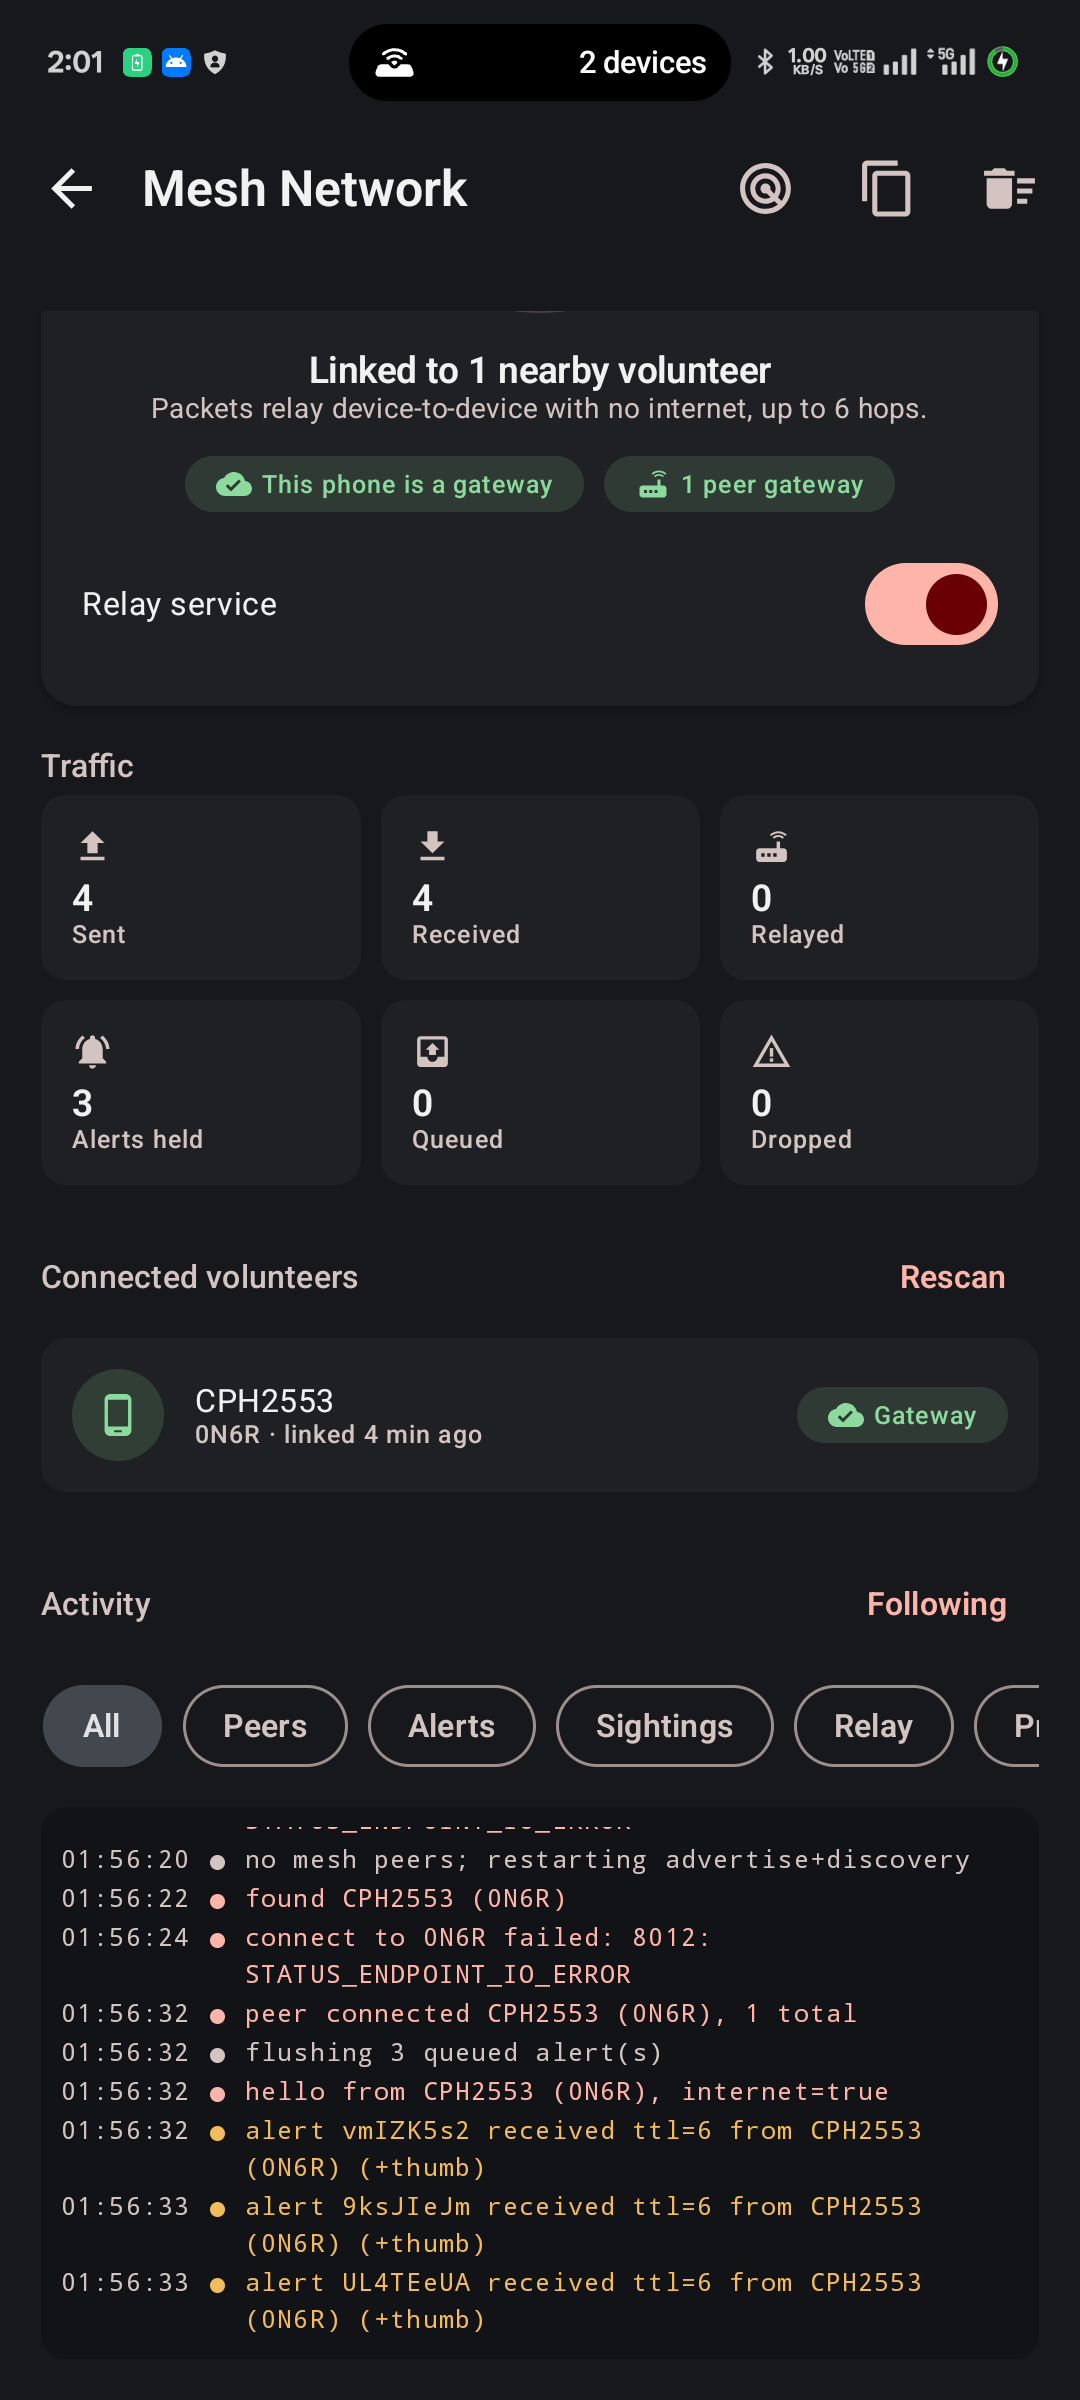
\includegraphics[width=\linewidth]{images/ss_16_mesh_log.png}
  \caption{16. Mesh activity log}
\end{subfigure}\hfill
\begin{subfigure}[t]{0.31\textwidth}
  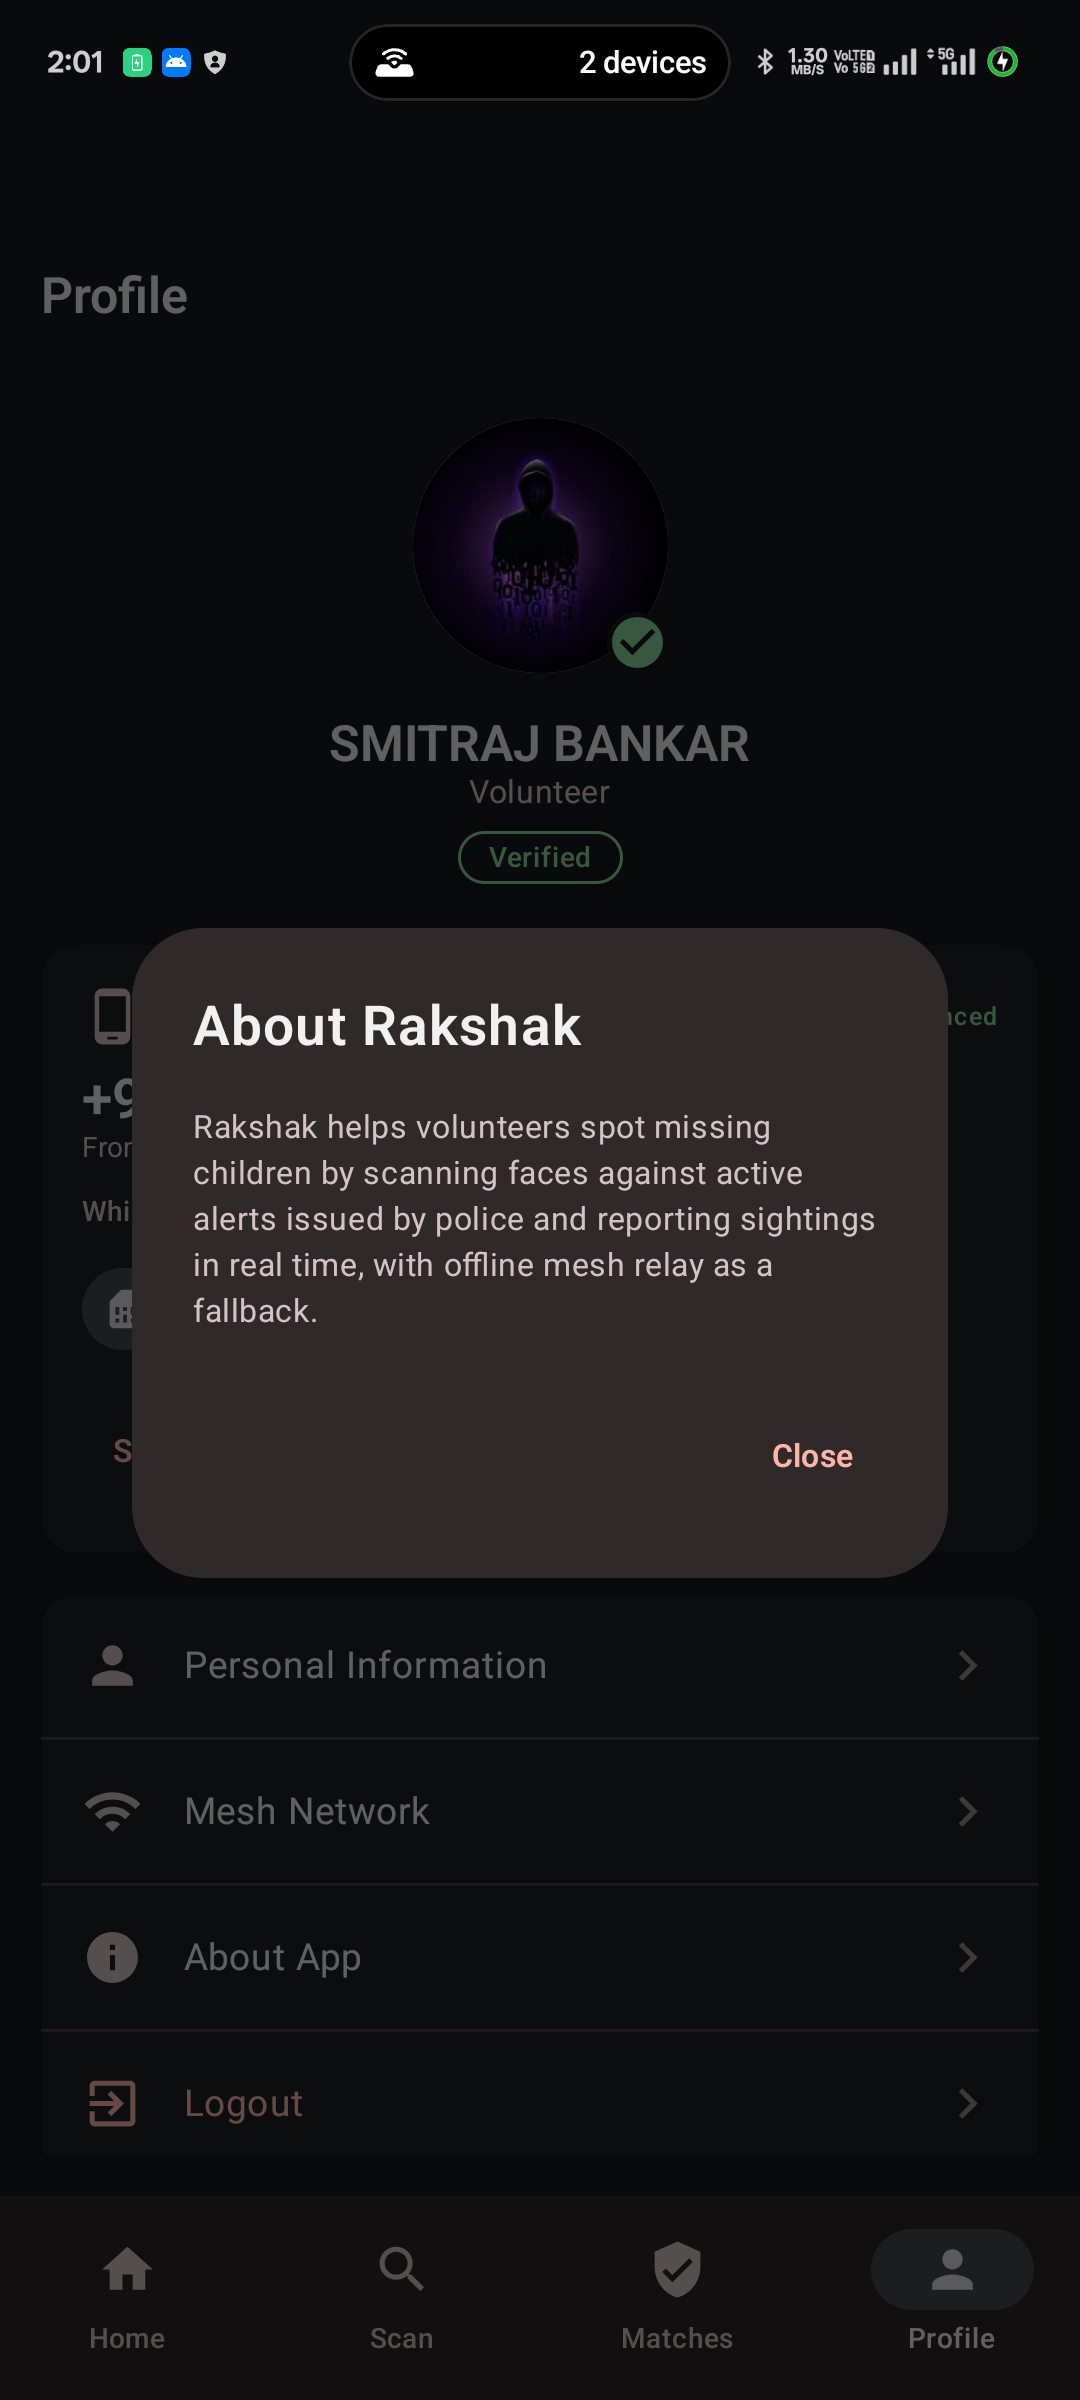
\includegraphics[width=\linewidth]{images/ss_17_about_app.png}
  \caption{17. About app}
\end{subfigure}\hfill
\begin{subfigure}[t]{0.31\textwidth}
  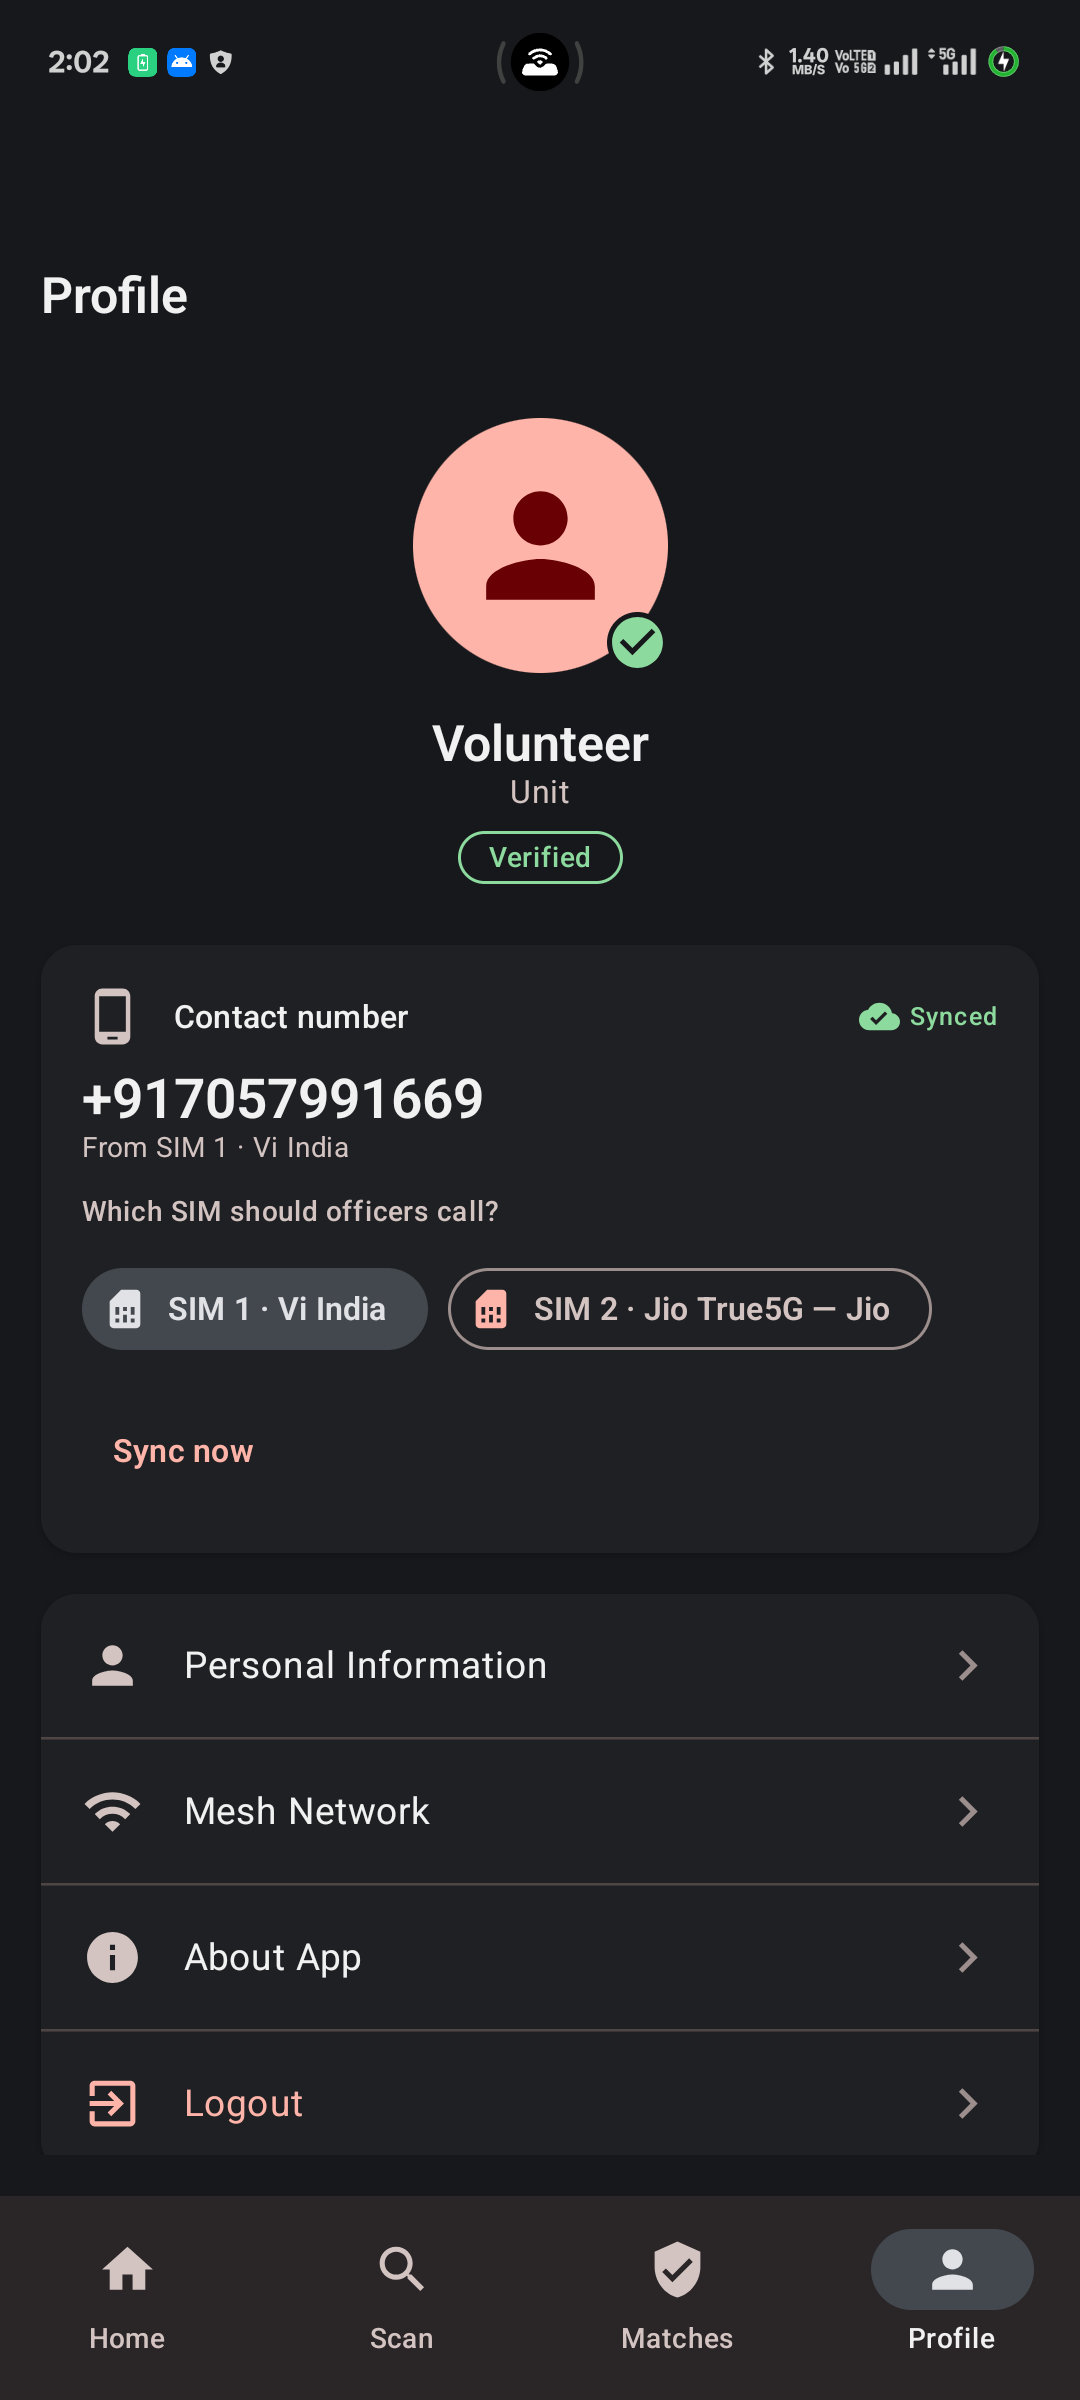
\includegraphics[width=\linewidth]{images/ss_18_logout_tapped.png}
  \caption{18. Logout tapped}
\end{subfigure}
\caption{Mobile workflow, screens 16--18: mesh log, about, and sign-out}
\label{fig:wf6}
\end{figure}

\begin{figure}[H]
\centering
\begin{subfigure}[t]{0.4\textwidth}
  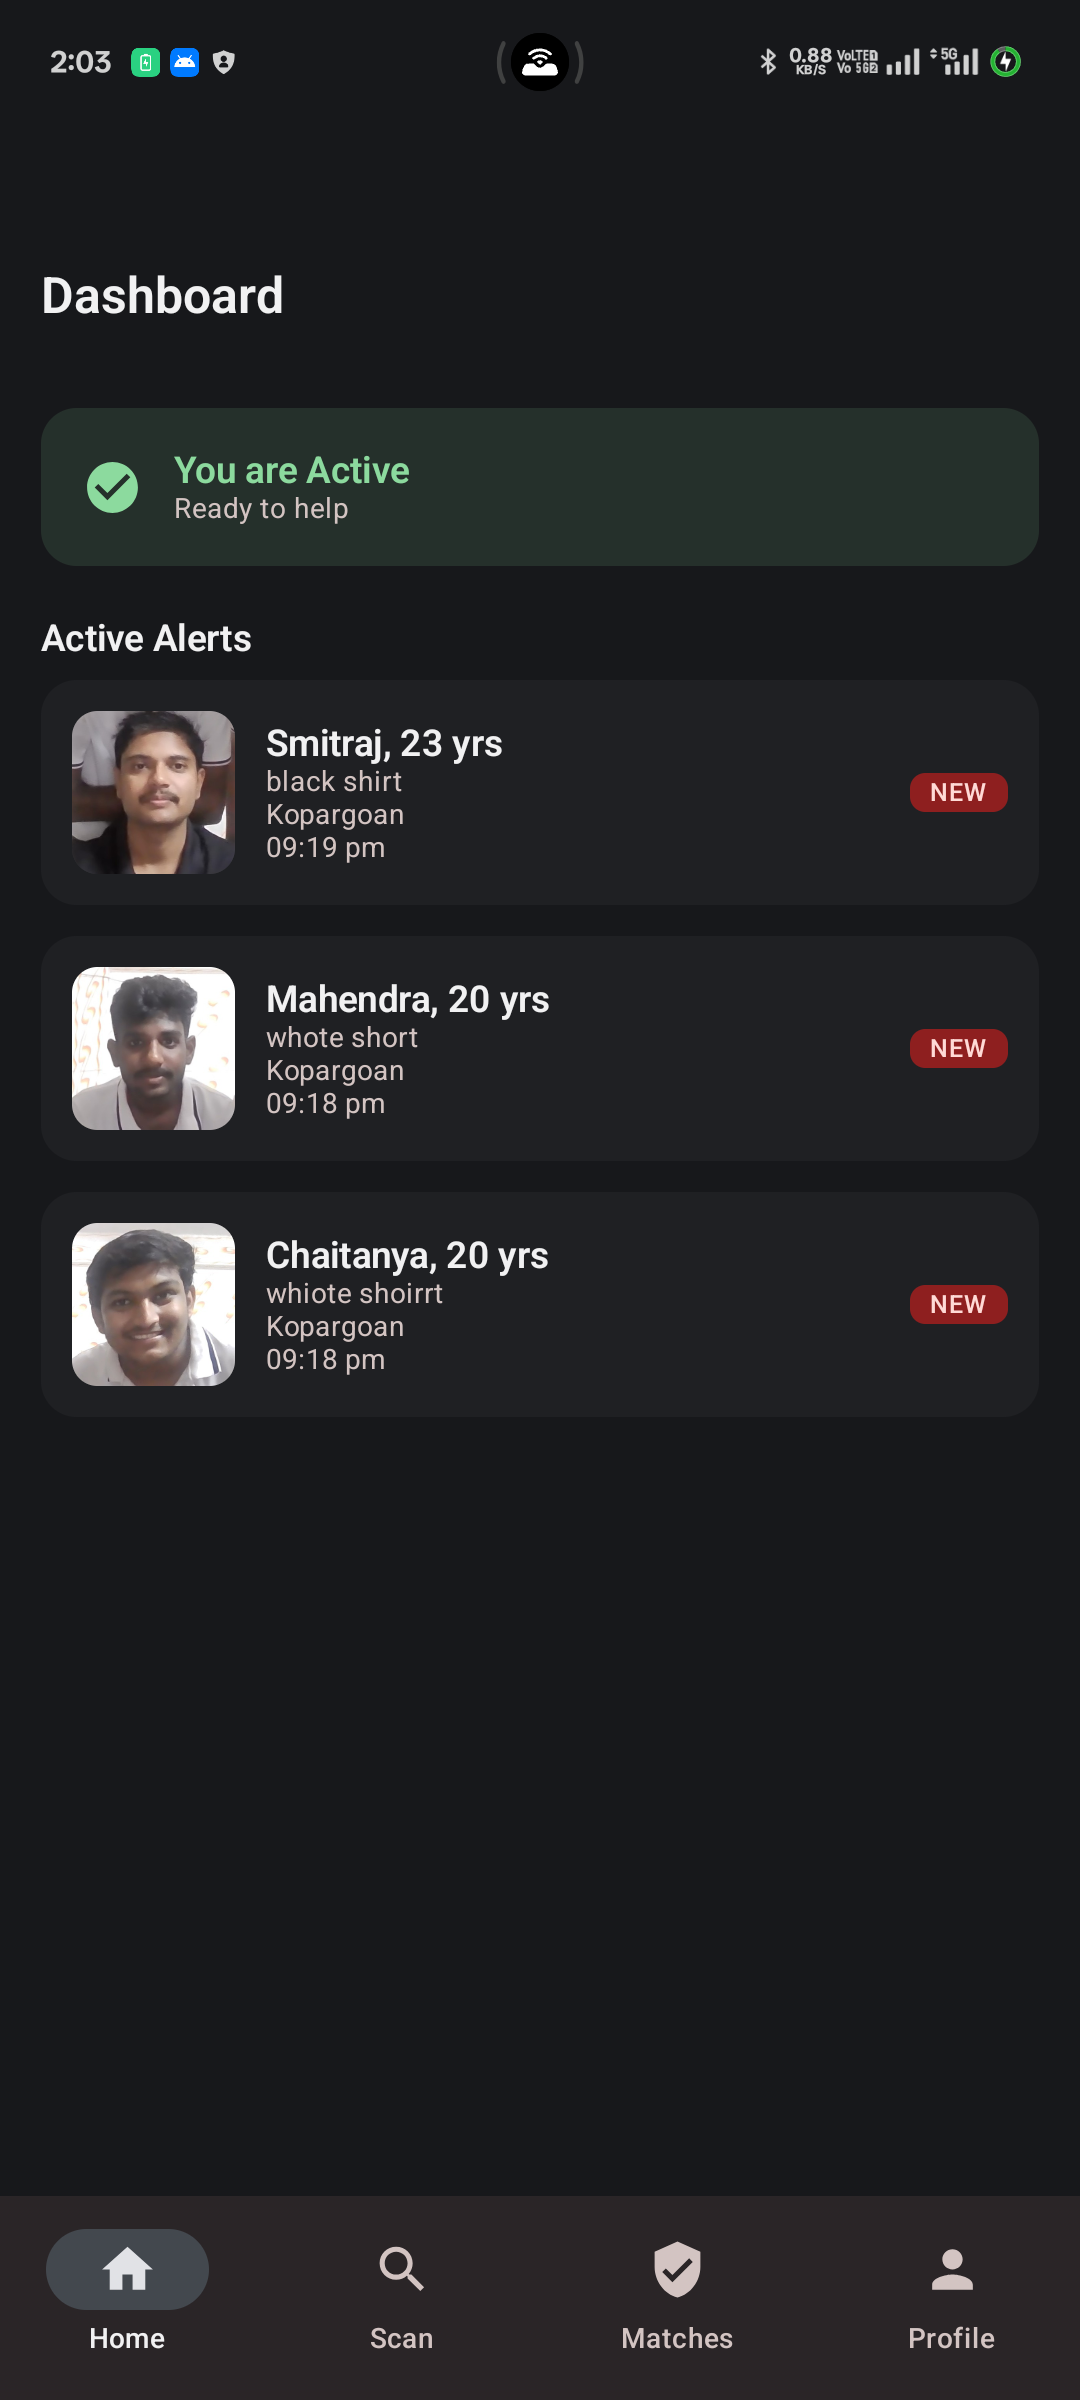
\includegraphics[width=\linewidth]{images/ss_19_final_home.png}
  \caption{19. Back at login after sign-out}
\end{subfigure}
\caption{Mobile workflow, screen 19: session end -- state restored to login}
\label{fig:wf7}
\end{figure}

\section{Cloud Functions and Data Coordination}

Coordination between the kiosk and every volunteer device runs entirely on
Firebase \cite{firebase} -- Firestore, Cloud Storage, Authentication, and
Cloud Messaging -- with six Cloud Functions doing the server-side work
neither client can do on its own.

\begin{table}[H]
\centering
\caption{Cloud Function exports and their trigger}
\label{tab:functions}
\begin{tabular}{|>{\raggedright\arraybackslash}p{4.3cm}|>{\raggedright\arraybackslash}p{2.6cm}|p{6.3cm}|}
\hline
\textbf{Function} & \textbf{Trigger} & \textbf{Responsibility} \\
\hline
\code{onAlertCreated} & Firestore create on \code{alerts} & Fallback embedding computation, geofenced FCM broadcast \\ \hline
\code{onMatchCreated} & Firestore create on \code{matches} & Push the confirmed sighting to the filing officer \\ \hline
\code{onAlertResolved} & Firestore update, active$\to$resolved & Purge embedding, alert photo, and every copied match photo URL \\ \hline
\code{expireAlerts} & Scheduled, every 30 min & Auto-resolve alerts older than the configured TTL (8 h) \\ \hline
\code{compute-}\linebreak\code{EmbeddingCallable} & Callable (officers only) & Re-index one alert's embedding on demand \\ \hline
\code{claimOfficerRole} & Callable & Grant the \code{police} claim and upsert the officer directory record \\
\hline
\end{tabular}
\end{table}

\subsection*{Geofenced broadcast}
\begin{lstlisting}[language=TypeScript, caption={Haversine geofence filter -- excerpt of \texttt{functions/src/notify.ts}}]
const GEOFENCE_RADIUS_KM = 2;
const STALE_LOCATION_MS = 6 * 60 * 60 * 1000;

function withinGeofence(alertLoc: GeoPoint, volunteerLoc: GeoPoint): boolean {
  const R = 6371; // Earth radius, km
  const dLat = toRad(volunteerLoc.latitude - alertLoc.latitude);
  const dLon = toRad(volunteerLoc.longitude - alertLoc.longitude);
  const a = Math.sin(dLat / 2) ** 2 +
    Math.cos(toRad(alertLoc.latitude)) * Math.cos(toRad(volunteerLoc.latitude)) *
    Math.sin(dLon / 2) ** 2;
  const distanceKm = 2 * R * Math.asin(Math.sqrt(a));
  return distanceKm <= GEOFENCE_RADIUS_KM;
}
// Fail-open: a volunteer is skipped only if their fix is valid AND fresh
// AND out of range -- a stale or missing fix never silently excludes them.
\end{lstlisting}

\subsection{Data Lifecycle -- Privacy Purge on Resolve}
\label{sec:privacy-purge}

This is where the project's privacy claim becomes enforceable code rather
than a policy statement. The moment an officer resolves a case (or the
scheduled 8-hour sweep does it for them), \code{onAlertResolved} deletes
the Storage object outright and clears every trace of the biometric vector:

\begin{lstlisting}[language=TypeScript, caption={Purge on resolve -- excerpt of \texttt{functions/src/index.ts}}]
export const onAlertResolved = onDocumentUpdated("alerts/{alertId}", async (event) => {
  const before = event.data?.before.data();
  const after = event.data?.after.data();
  if (before?.status !== "active" || after?.status !== "resolved") return;

  await storage.bucket().file(extractPath(after.imageUrl)).delete().catch(() => {});
  await event.data!.after.ref.update({ embedding: [], imageUrl: "" });

  // Every match copied this alert's photo URL for its own listener --
  // blank those too, or the kiosk shows a permanently broken image.
  const matches = await db.collection("matches")
    .where("alertId", "==", event.params.alertId).get();
  const batches = chunk(matches.docs, 500);       // Firestore batch limit
  for (const b of batches) {
    const batch = db.batch();
    b.forEach((m) => batch.update(m.ref, { imageUrl: "" }));
    await batch.commit();
  }
});
\end{lstlisting}

\code{expireAlerts} (a 30-minute scheduled function) reuses the same
chunked-batch pattern to flip every alert past its TTL to
\code{resolved} -- which in turn fires \code{onAlertResolved} for each one,
so a backlog of stale alerts cannot throw partway through and leave some
of them holding live biometric data.

\section{Offline Mesh Networking}
\label{sec:offline-mesh}

Google's Nearby Connections API \cite{nearby} links pairs of nearby devices
over Bluetooth Low Energy (discovery) and Wi-Fi Direct (transfer) -- it is
not itself a multi-hop mesh protocol. NextGen Rakshak implements a dedicated
application-level store-and-forward layer on top of it.

\begin{table}[H]
\centering
\caption{Mesh packet wire format}
\begin{tabular}{|p{3.0cm}|p{9.8cm}|}
\hline
\textbf{Field} & \textbf{Purpose} \\
\hline
TTL (1 byte) & Hop-count, initialised to 6, decremented per relay, packet dropped at 1 \\ \hline
Type tag (1 byte) & \code{alert} $\mid$ \code{match} $\mid$ \code{resolve} $\mid$ \code{hello} $\mid$ \code{ack} \\ \hline
Message ID (UUID) & Uniquely identifies the packet so a device relays it at most once \\ \hline
Payload & Type-specific fields: alert text fields, embedding vector, $\leq$8\,KB face thumbnail (alert); GPS + confidence (match) \\ \hline
HMAC-SHA256 trailer (32 bytes) & Authenticates everything except the mutable TTL byte; a packet that fails verification is dropped before parsing \\
\hline
\end{tabular}
\end{table}

\begin{lstlisting}[language=Kotlin, caption={Relay guard -- simplified from \texttt{networking/\allowbreak mesh/\allowbreak MeshNetworkManager.kt}}]
fun onPacketReceived(raw: ByteArray, fromEndpoint: String) {
    val packet = MeshPayloadCodec.decode(raw) ?: return         // bad HMAC -> drop
    if (seenCache.contains(packet.messageId)) return             // already relayed
    seenCache.remember(packet.messageId, ttlMillis = ALERT_LIFETIME_MS)

    handleLocally(packet)                                        // update UI/state

    if (packet.ttl > 1) {
        val relay = packet.copy(ttl = packet.ttl - 1)
        connectedEndpoints.filter { it != fromEndpoint }
            .forEach { sendPayload(it, MeshPayloadCodec.encode(relay)) }
    }
}
\end{lstlisting}

\begin{figure}[H]
\centering
\begin{subfigure}[t]{0.48\textwidth}
  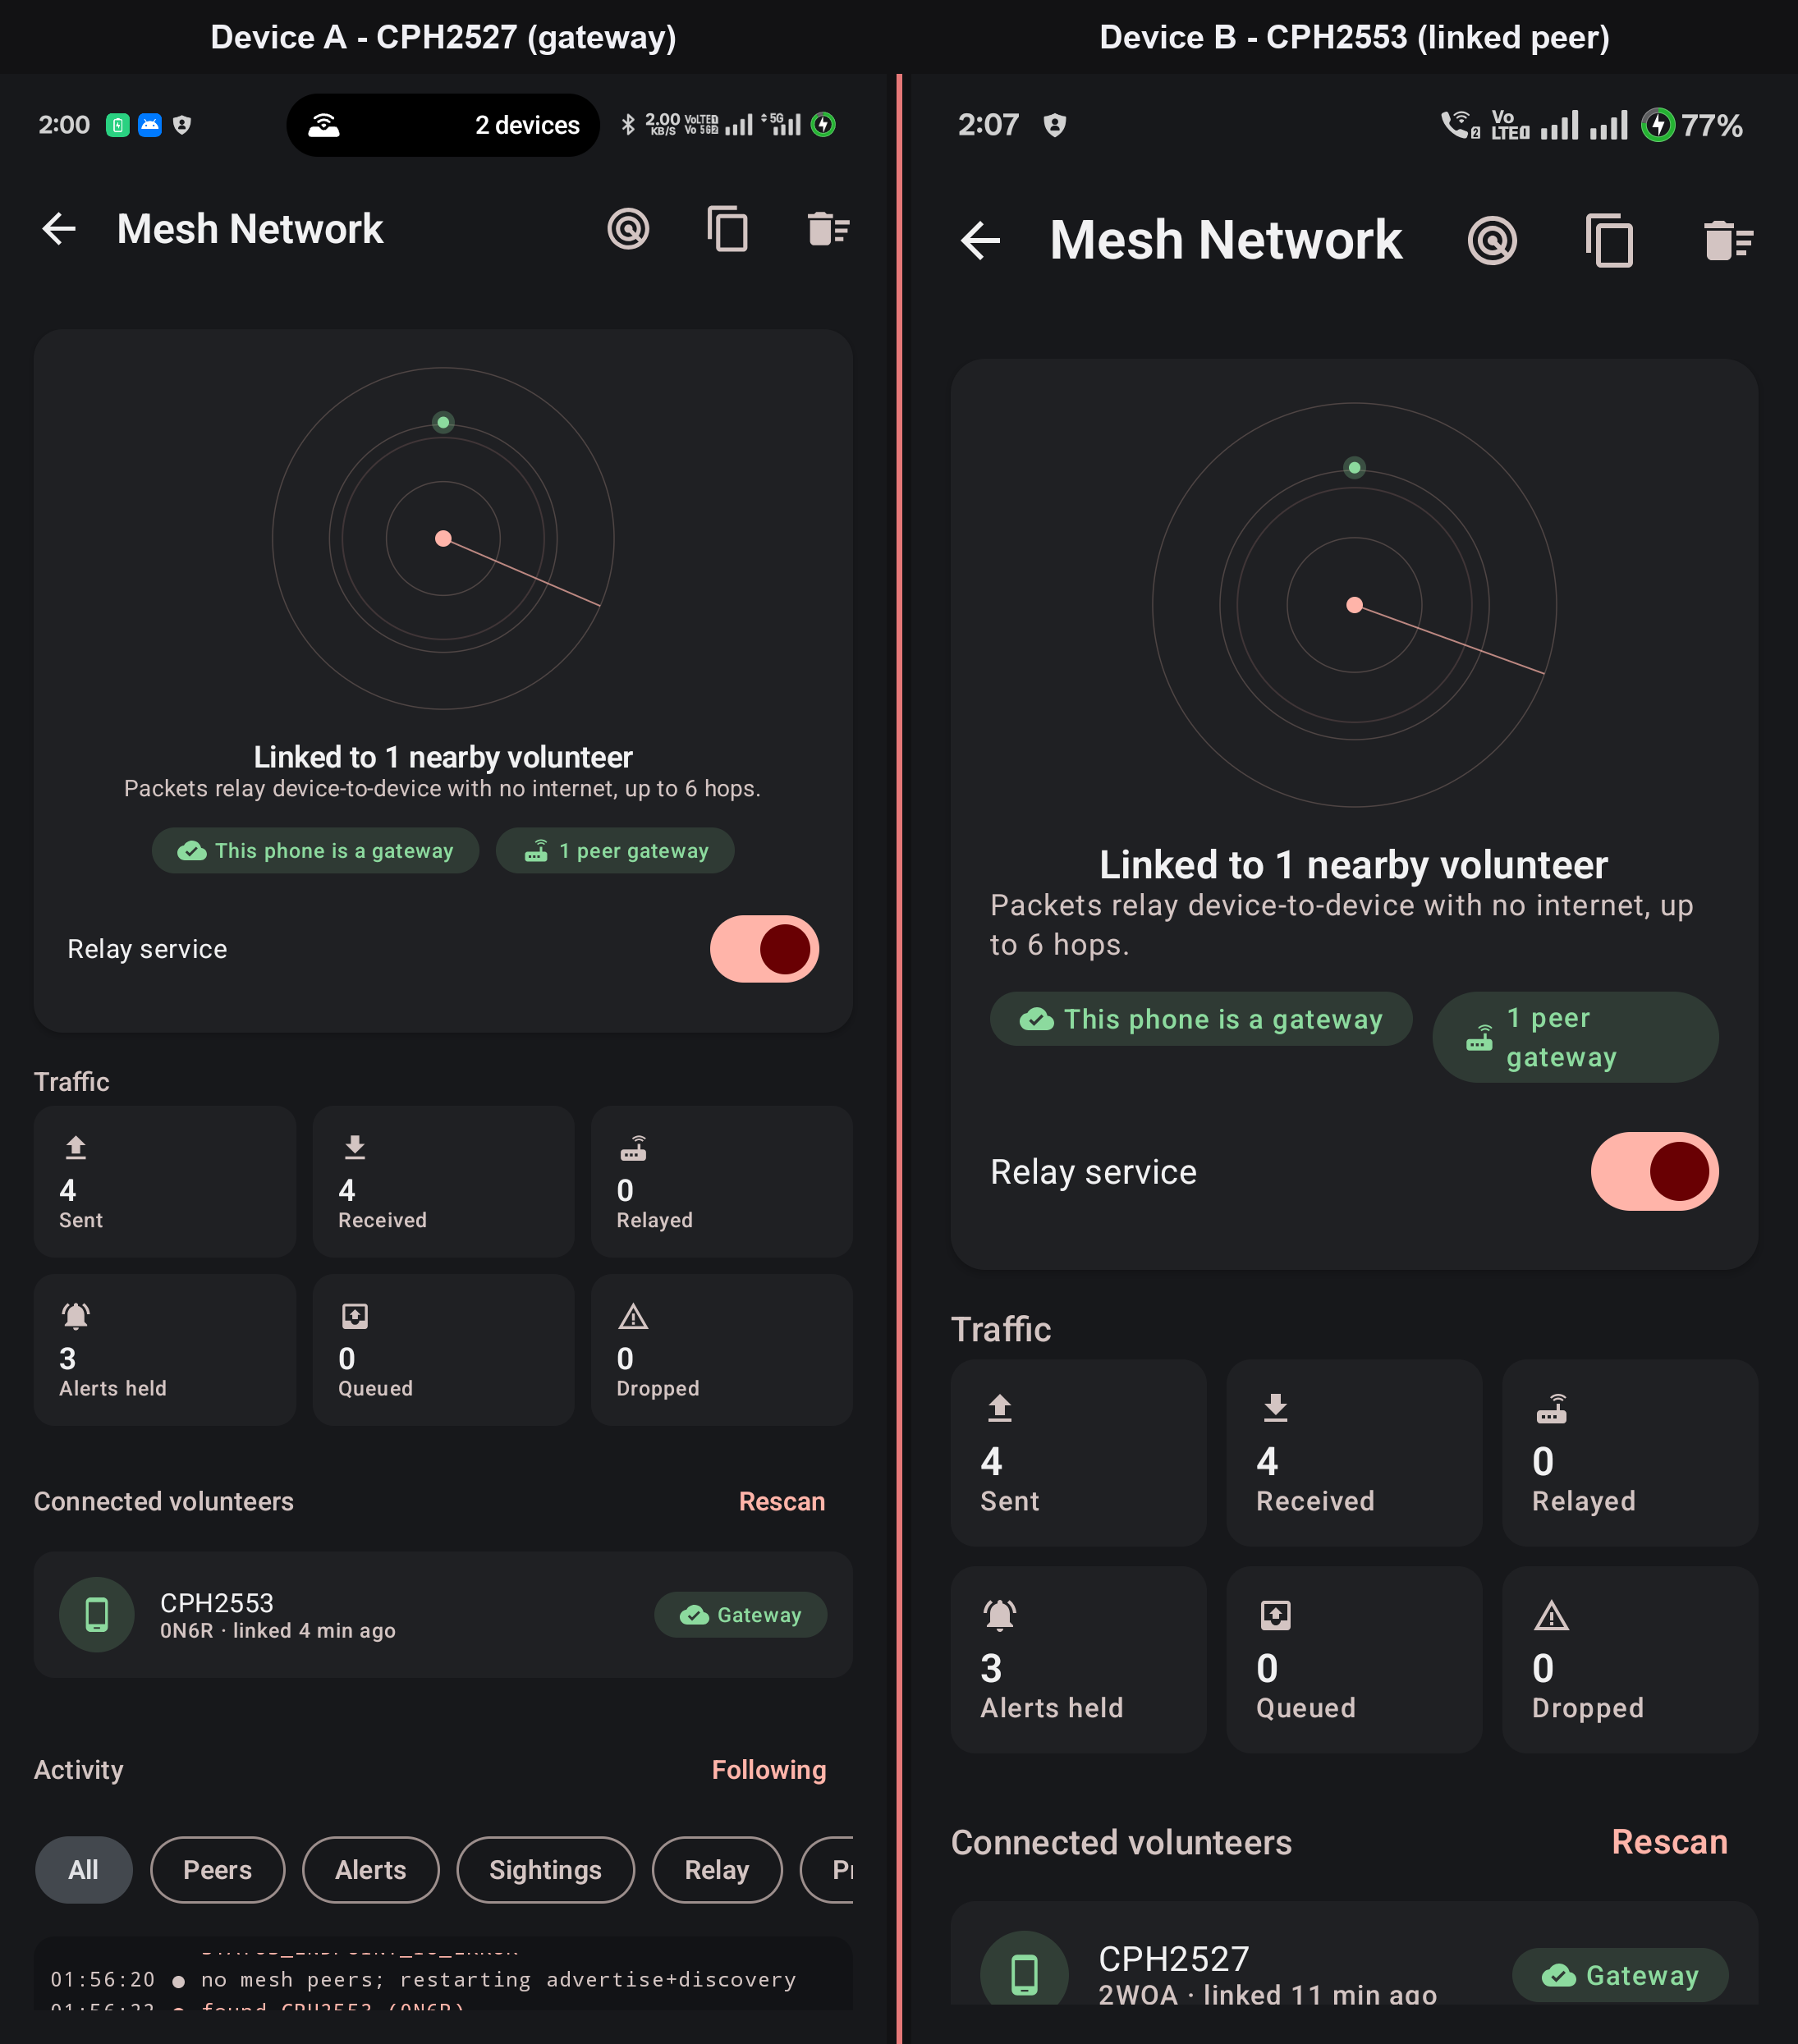
\includegraphics[width=\linewidth]{images/ss_15_mesh_compare.png}
  \caption{Mesh network screen -- peer status}
\end{subfigure}\hfill
\begin{subfigure}[t]{0.48\textwidth}
  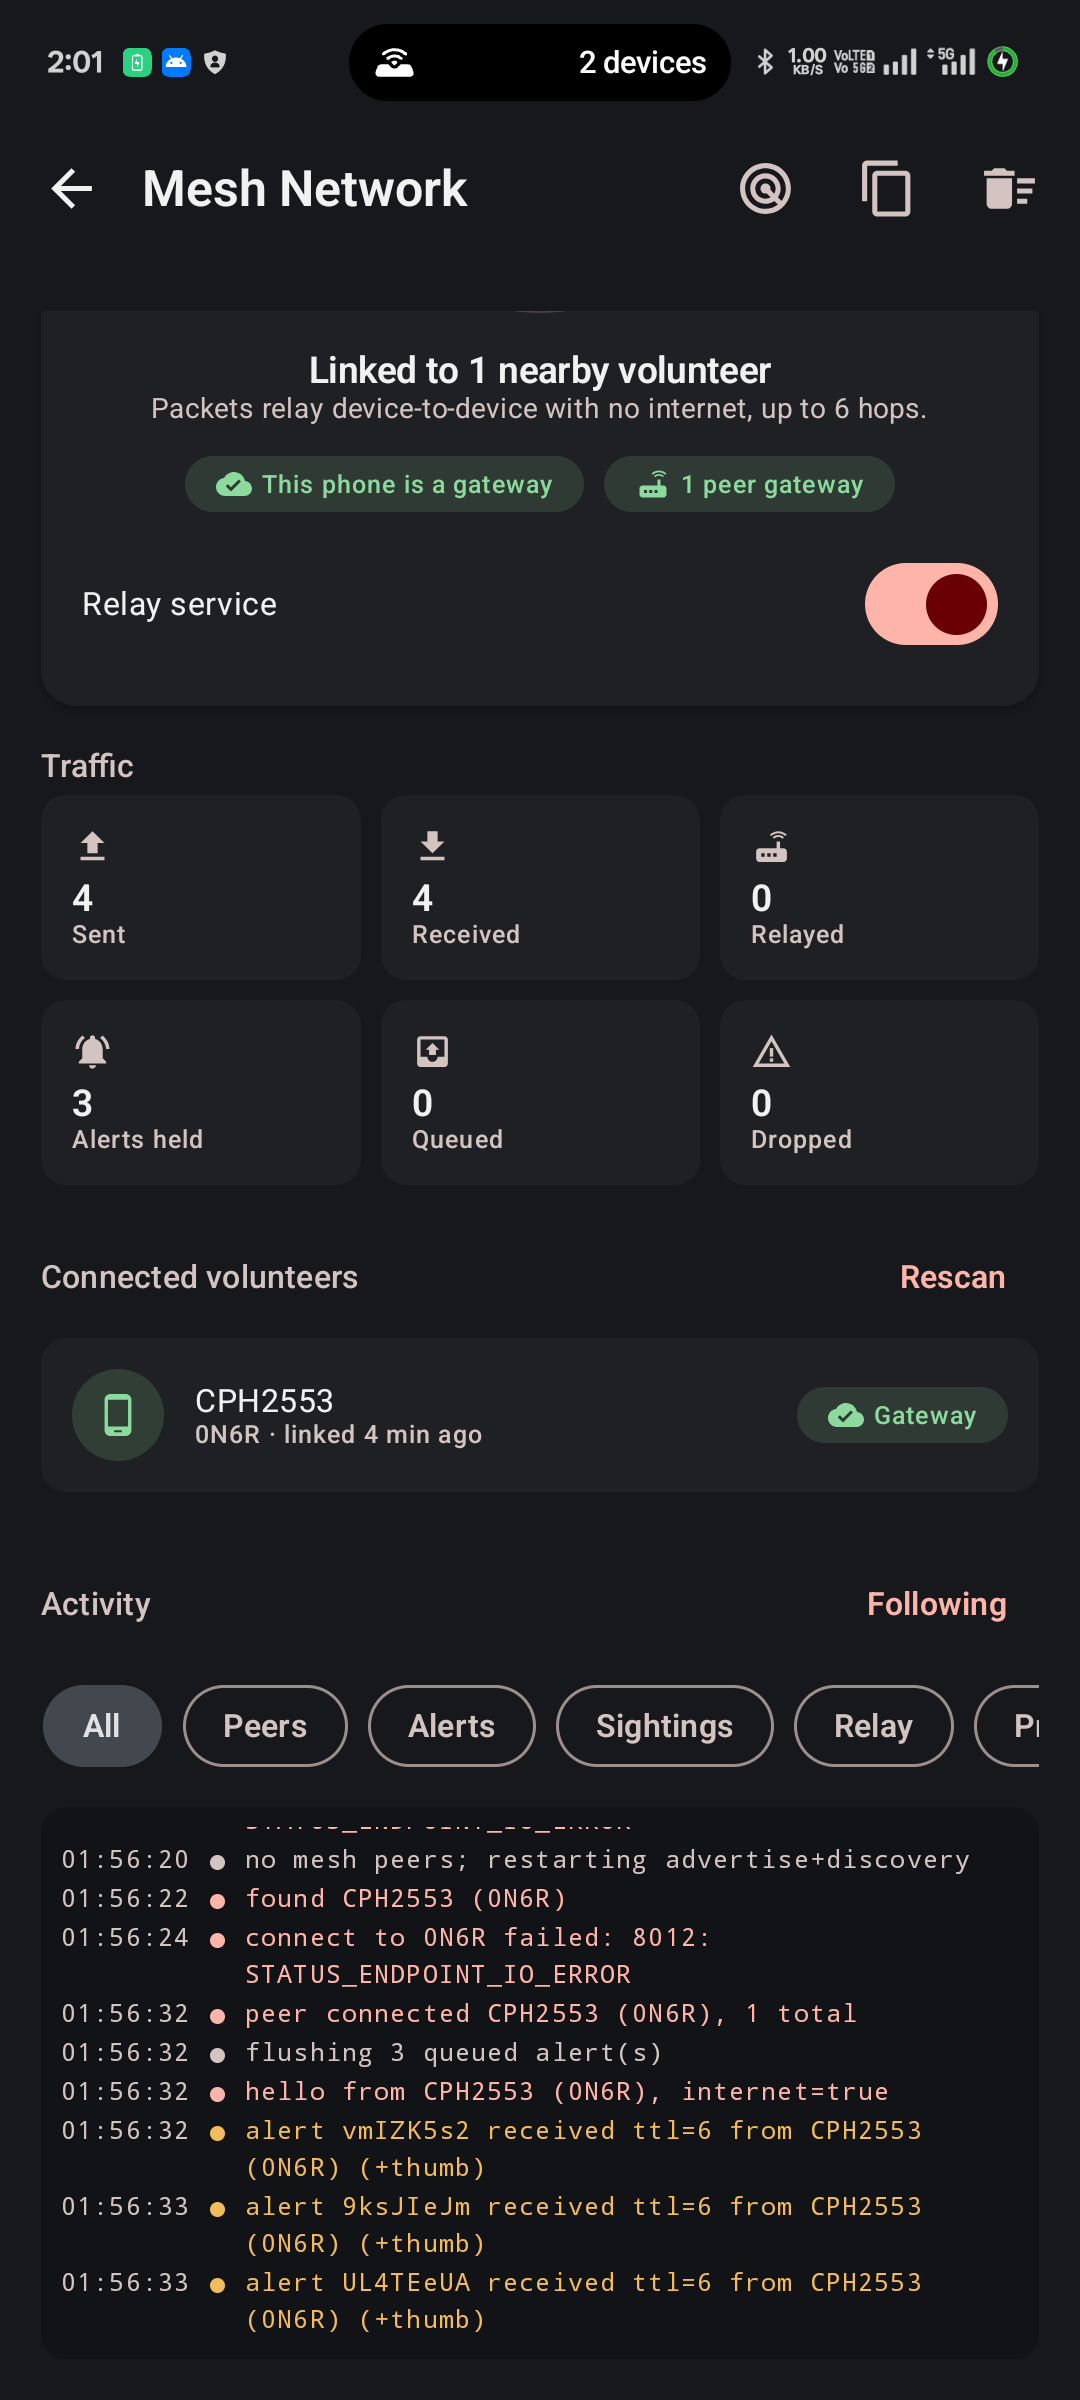
\includegraphics[width=\linewidth]{images/ss_16_mesh_log.png}
  \caption{Mesh activity log -- packet-level trace}
\end{subfigure}
\caption{Offline mesh -- live visualisation on the volunteer app}
\end{figure}

\label{sec:mesh-reconnect}
A three-physical-device field trial confirmed genuine multi-hop relay: an
alert was traced hopping two links deep (TTL decrementing $6\rightarrow5$)
between two phones that were never directly paired, over a star topology
formed by Nearby's own discovery timing. The trial also surfaced and fixed
two reconnect-stability defects invisible to unit tests -- a missing
run-time \code{NEARBY\_WIFI\_DEVICES} permission request on Android 13+, and
a discovery-only ``endpoint lost'' callback that was incorrectly wired to
the same logic as a genuine disconnect, zeroing the peer count for a link
that was in fact still alive.

\section{Security Implementation}
\label{sec:security}

Firestore security rules enforce every authorisation boundary
server-side -- the client-side route guard is a UX convenience, not the
security boundary.

\begin{lstlisting}[language=JavaScript, caption={Firestore rule excerpt -- alerts and matches (\texttt{firestore.rules})}]
match /alerts/{alertId} {
  allow read: if request.auth != null;
  allow create: if isPolice() && request.resource.data.createdBy.uid == request.auth.uid;
  allow update: if isPolice();
  allow delete: if false;
}

match /matches/{matchId} {
  allow read: if request.auth != null;
  allow create: if request.auth != null && validMatch() && attributed();
  allow update: if isPolice() &&
    request.resource.data.diff(resource.data).affectedKeys().hasOnly(['status']) &&
    request.resource.data.status in ['pending','dispatched','accepted','dismissed'];
  allow delete: if false;
}
\end{lstlisting}

\section{Deployment}
\label{sec:deployment}

The police kiosk portal is deployed and publicly reachable at
\url{https://nextgen-rakshak.vercel.app/} -- this is not a local
development build; it is the same production build the testing in
\S\ref{sec:field-trial} and Table~\ref{tab:testcases} was carried out
against. Each of the project's three components is deployed separately,
matching the three-layer architecture in Figure~\ref{fig:arch}.

\subsection{Police Kiosk Portal -- Vercel}

The kiosk is a standard Next.js 14 App Router project, which Vercel builds
with zero custom configuration.

\begin{enumerate}
  \item The GitHub repository (\S4.1.2) is connected to a Vercel project,
        with the project root set to: \\
        \texttt{nextgen-rakshak-webportal/}.
  \item The Firebase web SDK configuration is supplied as environment
        variables in the Vercel project settings -- never committed to the
        repository -- covering the API key, auth domain, project ID,
        storage bucket, messaging sender ID, app ID, and the Cloud
        Messaging VAPID key the notification bell needs for push.
  \item Vercel runs \code{next build} against these variables and deploys
        the result to its edge network; every push to \code{main} triggers
        a fresh production deployment automatically, with no manual step.
  \item The Firebase project's Authentication settings are configured to
        accept the deployed domain (\texttt{nextgen-rakshak.vercel.app}) as
        an authorised OAuth redirect origin for Google sign-in.
\end{enumerate}

\subsection{Cloud Functions, Firestore Rules, and Storage Rules -- Firebase}

The backend is deployed independently of the kiosk, directly from the
\texttt{functions/} workspace, via the Firebase CLI:

\begin{lstlisting}[caption={Backend deployment command}]
cd functions && npm install
firebase deploy --only functions,firestore:rules,firestore:indexes,storage:rules
\end{lstlisting}

This single command pushes all six Cloud Functions (Table~\ref{tab:functions}),
the Firestore security rules (\S\ref{sec:security}), the composite index, and the Storage
rules together, so the rules and the functions that assume them are always
deployed as one atomic unit rather than drifting apart.

\subsection{Volunteer Android App -- Signed Release APK}

The volunteer app is not distributed through the Play Store; it is
sideloaded as a signed release APK, which is the standard distribution
model for a final-year field trial.

\begin{enumerate}
  \item \code{google-services.json} for the same Firebase project is
        placed in the mobile app's module directory: \\
        \texttt{nextgen-rakshak-mobile/app/}.
  \item The release signing key's SHA-1 is registered against the Firebase
        Android app, and \code{MESH\_HMAC\_KEY} is set in
        \texttt{local.properties} -- a release build refuses to compile
        with the well-known development key (\S\ref{sec:offline-mesh}), so this step cannot
        be silently skipped.
  \item \code{./gradlew :app:assembleRelease} produces the signed APK,
        which was installed directly on the field-trial devices used in
        \S\ref{sec:field-trial}.
\end{enumerate}

\noindent All three deployments share one Firebase project, so a change to
the Firestore schema or security rules takes effect for the live kiosk and
every installed copy of the app simultaneously.

\section{Testing, Field Validation, and Results}

\subsection{Testing Strategy}

Four layers of testing were used, matching the four things that can
independently break in a system this shape: the matching logic itself, the
mesh's packet handling, the full stack wired together, and the stack
running on real, physically separate hardware rather than an emulator.

\begin{itemize}
  \item \textbf{Unit testing} -- the matching and mesh-networking logic,
        which is pure computation with no Android framework dependency, is
        covered by the JVM test suite in \S\ref{sec:unit-tests}.
  \item \textbf{Integration testing} -- each Cloud Function was exercised
        against a live Firestore project (alert create $\to$ embedding
        $\to$ geofenced push $\to$ match create $\to$ officer push), and the
        kiosk's data-API layer (\S\ref{sec:kiosk-data-api}) against the deployed rules.
  \item \textbf{System testing} -- the full alert-to-dispatch path was
        walked manually on real Android hardware for every functional
        requirement in Table~\ref{tab:fr} at least once (Table~\ref{tab:testcases}).
  \item \textbf{Field testing} -- the offline mesh was run across
        physically separate phones outside the emulator, since Nearby
        Connections' BLE/Wi-Fi Direct behaviour cannot be simulated
        (\S\ref{sec:field-trial}).
\end{itemize}

\subsection{Unit Test Suite}
\label{sec:unit-tests}

The volunteer app's core matching and mesh logic is covered by unit tests,
run through \code{./gradlew :app:testDebugUnitTest}:

\begin{table}[H]
\centering
\caption{Unit test suite -- volunteer Android app}
\begin{tabular}{|p{6.0cm}|p{6.0cm}|}
\hline
\textbf{Matching / geometry} & \textbf{Mesh networking} \\
\hline
\code{CosineEmbeddingComparatorTest} & \code{MeshCryptoTest} \\ \hline
\code{AlertIndexTest} & \code{MeshPayloadCodecTest} \\ \hline
\code{EmbeddingAggregatorTest} & \code{MeshRouterTest} \\ \hline
\code{TrackRegistryTest} & \code{MeshSeenCacheTest} \\ \hline
\code{FaceGeometryTest} & \code{MeshAlertSourceTest} \\ \hline
\code{ElapsedTimeTest} & \\
\hline
\end{tabular}
\end{table}

\subsection{System Test Cases}

Every row below was executed manually on real Android hardware (not the
emulator) against the deployed Firebase project, not a mock backend.
Results are reported as observed -- a defect \emph{found} during this pass
is reported as found, with the fix that followed it, rather than silently
retested until it disappears from the table.

\begin{longtable}{|p{1.0cm}|p{5.9cm}|p{5.7cm}|}
\caption{System-level test cases, executed on real hardware}
\label{tab:testcases}\\
\hline
\textbf{ID} & \textbf{Scenario} & \textbf{Result} \\
\hline
\endfirsthead
\hline
\textbf{ID} & \textbf{Scenario} & \textbf{Result} \\
\hline
\endhead
TC-01 & Officer sign-in is gated on the \code{police} custom claim, not merely being signed in (FR) & \textbf{Pass} -- a non-claimed Google account is refused; \code{claimOfficerRole} grants access on first legitimate sign-in \\ \hline
TC-02 & Officer files an alert with photo + structured details (FR-01) & \textbf{Pass} -- \code{alerts} document created, photo stored, geolocation captured \\ \hline
TC-03 & Fallback embedding computed server-side on alert creation (FR-02) & \textbf{Pass} -- \code{onAlertCreated} writes the embedding within the Cloud Function's cold/warm response window \\ \hline
TC-04 & Geofenced push reaches volunteers within 2\,km of the kiosk (FR-03) & \textbf{Pass} -- FCM notification observed on the volunteer device end-to-end \\ \hline
TC-05 & On-device face detection with the frontality gate rejects extreme head-pose (FR-04) & \textbf{Pass} -- verified on real device under normal indoor lighting \\ \hline
TC-06 & On-device embedding + cosine comparison against the active alert (FR-05, FR-06) & \textbf{Pass} -- a genuine live match was observed at $\sim$77\% cosine confidence on real hardware \\ \hline
TC-07 & Side-by-side confirmation dialog, including the offline-thumbnail fallback (FR-07) & \textbf{Pass} -- dialog renders the parent's photo beside the live camera crop in both the online and mesh-only paths \\ \hline
TC-08 & Volunteer explicitly confirms or dismisses a candidate (FR-08) & \textbf{Pass} -- both branches verified; a dismissal returns to scanning without reporting \\ \hline
TC-09 & Confirmed sighting reaches the kiosk with a GPS fix (FR-09) & \textbf{Pass} -- match appears on the officer's live feed with location \\ \hline
TC-10 & Alert auto-expiry after 8\,h (FR-12) & \textbf{Partial} -- scheduled sweep deployed and observed to fire; not stopwatched end-to-end against a live 8-hour case \\ \hline
TC-11 & 2-device offline mesh relay, no internet on either device (FR-10) & \textbf{Pass} -- alert and match propagate phone-to-phone; confirmed by unit test and by hand \\ \hline
TC-12 & 3-device offline mesh relay, multi-hop, no internet anywhere (FR-10) & \textbf{Pass} -- see the field trial, \S\ref{sec:field-trial} \\ \hline
TC-13 & Regression: comparing a centred-crop embedding against a 3-point-aligned embedding of the \emph{same} face (geometry mismatch) & \textbf{Defect found} -- scored 0.38--0.49, below the 0.55 threshold, for an identical face. \textbf{Fixed} by re-embedding every alert photo on-device (\S\ref{sec:reembed}) \\ \hline
TC-14 & Sustained continuous scanning under load (interpreter concurrency) & \textbf{Defect found} -- a race in the interpreter gate could deadlock a second concurrent call. \textbf{Fixed}; see \S\ref{sec:concurrency-safety} \\ \hline
TC-15 & Mesh discovery/advertising on a fresh 3-device session (Android 13+ permissions, spurious disconnects) & \textbf{2 defects found and fixed} -- missing runtime \code{NEARBY\_WIFI\_DEVICES} request, and a discovery callback wrongly wired to disconnect logic; see \S\ref{sec:field-trial} \\ \hline
TC-16 & 50 concurrent active alerts (NFR-07) & \textbf{Not yet tested} -- open, requires a dedicated multi-alert load rig \\ \hline
TC-17 & Recognition accuracy specifically on children's faces (NFR-02) & \textbf{Not yet tested} -- open; see Future Scope (\S9.2) for the ethical/dataset constraint \\
\hline
\end{longtable}

\textbf{Result summary:} 12 of 17 system-level test cases passed outright,
3 uncovered real defects that were fixed as a direct result of testing
(TC-13, TC-14, TC-15 -- arguably testing's most valuable output), 1 is
partially verified (TC-10), and 2 remain explicitly open (TC-16, TC-17),
matching the same items already flagged open in Table~\ref{tab:nfr} --
nothing here is reported as passing that is not also reflected there.

\subsection{Field Trial -- Offline Mesh on Three Physical Devices}
\label{sec:field-trial}

The single hardest claim in this project to fake and the single most
important one to verify honestly is that the offline mesh actually
relays across more than one hop on real hardware, since Nearby
Connections' BLE discovery and Wi-Fi Direct transfer behaviour cannot be
meaningfully reproduced on an emulator.

\textbf{Setup:} three physical Android phones, airplane mode with only
Bluetooth and Wi-Fi enabled (no cellular, no internet on any device), the
release APK signed with the production \code{MESH\_HMAC\_KEY}, all three
in Nearby-discovery range of at least one other device.

\textbf{What was tested:} an alert filed on one device's mesh queue, left
to propagate device-to-device with no direct pairing forced between all
three; a confirmed match relayed back the same way; and the system left
running long enough to observe reconnect behaviour, not just a single
successful hop.

\textbf{Result:} a relayed alert was traced hopping two links deep -- the
TTL byte decrementing $6\rightarrow5$ across two devices confirmed never to
be directly paired with each other -- proving genuine multi-hop relay
rather than a single Nearby Connections link. The three phones held a
stable mesh in a star topology (which device links to which is decided by
Nearby's own discovery timing, not by the app) for the length of the
trial.

The trial also did what field trials are supposed to do: it found two real
defects invisible to both unit tests and single-device testing.

\begin{enumerate}
  \item \code{NEARBY\_WIFI\_DEVICES} was declared in the Android manifest
        but never actually requested at runtime. On Android 13+, a device
        without it pre-granted could be \emph{found} by another device's
        discovery but could never run its own discovery -- silently and
        permanently, with only a permission-denied log line as evidence.
        Fixed by adding it to the app's runtime permission request.
  \item \code{onEndpointLost} -- a discovery-layer callback meaning "this
        BLE beacon is no longer visible," not a real disconnect -- was
        wired to the same logic as a genuine
        \code{ConnectionLifecycleCallback.onDisconnected}. Nearby routinely
        throttles advertising once two devices are already paired, which
        fired this callback for links that were, per the system's own
        connection log, still exchanging keep-alive traffic successfully
        in both directions. This was silently zeroing the peer count --
        and the match-relay path with it -- for connections that were
        never actually down. Fixed by decoupling the two callbacks and
        adding a watchdog that re-arms discovery only when a device
        genuinely has zero peers.
\end{enumerate}

Both fixes shipped before the mesh was considered field-verified rather
than merely unit-tested. The remaining open item is measuring hop-relay
\emph{timing} under load with more devices (NFR-05), not whether the mesh
holds together at all -- that question is answered.

% ============================================================================
%  CHAPTER 8 -- APPLICATIONS OF THE PROJECT
% ============================================================================
\chapter{Applications of the Project}

While designed around the missing-child, golden-hour use case, the
underlying architecture -- geofenced alert distribution, on-device face
matching, and an offline mesh fallback -- generalises to several adjacent
public-safety scenarios:

\begin{itemize}
  \item \textbf{Religious and cultural mass gatherings} -- Kumbh Mela,
        Dussehra processions, Ganesh Chaturthi visarjan, and urban temple
        fairs, the primary target scenario, where crowd density and network
        congestion are both at their peak simultaneously.
  \item \textbf{School and college excursions} -- a teacher-in-charge can
        file an alert for a separated student at a crowded destination
        (a zoo, an exhibition, a pilgrimage trip) using the same kiosk-style
        flow with chaperones as volunteers.
  \item \textbf{Large-scale public events} -- concerts, sporting events, and
        political rallies, where organised security staff already play the
        pre-registered-volunteer role the system assumes.
  \item \textbf{Disaster-response and relief camps} -- family separation
        during evacuation is a documented secondary harm in disaster
        response; the offline mesh is directly applicable where
        infrastructure damage has taken cellular networks down entirely.
  \item \textbf{Elderly and dementia-patient recovery} -- the same
        photo-embedding-and-match flow applies unchanged to a vulnerable
        adult who has wandered from a caregiver at a large event.
  \item \textbf{Exit-gate perimeter monitoring} -- the optional Raspberry Pi
        node extends the same on-device matching pipeline to a fixed,
        unattended camera at a controlled gate, complementing mobile
        volunteer coverage.
\end{itemize}

% ============================================================================
%  CHAPTER 9 -- CONCLUSION & FUTURE SCOPE
% ============================================================================
\chapter{Conclusion and Future Scope}

\section{Conclusion}

NextGen Rakshak set out to answer a narrow but consequential question: can a
system built entirely on smartphones already carried by ordinary volunteers
recover a missing child faster than the centralised, internet-dependent,
reactive tools currently deployed at Indian mass gatherings, without
uploading a single bystander's face to do it? The project's central design
decision -- moving all face recognition on-device and treating the cloud
purely as a coordination layer -- was carried through consistently across
all three components: a Next.js police kiosk for filing and reviewing
alerts, a Kotlin/Compose volunteer app that detects, aligns, embeds, and
matches faces entirely locally, and Firebase Cloud Functions that route
alerts and confirmed sightings without ever seeing a bystander's image.
The kiosk is not merely a local demo build: it is deployed and publicly
reachable at \url{https://nextgen-rakshak.vercel.app/} (\S\ref{sec:deployment}),
the same production deployment the field testing in this report was
carried out against.

Every functional requirement traced to the six project objectives
(Table~\ref{tab:fr}) was built, and the great majority were verified on
real Android hardware, including the two hardest claims in the literature
gap analysis: fully on-device face matching (verified with a live,
measured match at $\sim$77\% confidence) and genuine multi-hop offline
relay across three physically separate devices (verified with a traced,
two-hop packet). The face-matching threshold itself was derived from
measurement rather than assumed from a paper, and that measurement
discipline surfaced and fixed two subtle correctness defects -- a
geometry-mismatch bug that silently disabled matching, and two
mesh-reconnect bugs invisible to unit tests -- that would otherwise have
undermined the system's central claims in exactly the conditions a real
deployment would expose them.

Equally important to an honest final-year report is what remains open. The
non-functional targets in Table~\ref{tab:nfr} that require sustained,
large-scale field conditions -- 50 concurrent alerts, a formal children's-face
accuracy study, and mesh delivery timing beyond three devices -- are stated
here as unmeasured rather than claimed, consistent with the project's
guiding principle throughout: a documented limitation, explained, is worth
more than an unverified claim.

\section{Future Scope}

\begin{enumerate}
  \item \textbf{$\geq$3-device mesh field trial at scale} -- extend the
        three-device trial already completed to 8--10 devices to measure
        real-world hop-relay timing (NFR-05) rather than a single traced
        path.
  \item \textbf{Ethically sourced children's face dataset} -- pursue a
        licensed academic dataset or IRB-style consented data collection
        to validate NFR-02 on the system's actual target population, not
        an adult proxy.
  \item \textbf{Per-alert asymmetric signing} -- extend the current
        HMAC-based mesh packet authentication (a shared per-deployment key)
        with a public-key signature from the kiosk, so a relayed packet's
        \emph{origin} is verifiable, not merely its integrity.
  \item \textbf{Concurrency and load testing} -- formally benchmark the
        system against 50 simultaneous active alerts (NFR-07) and 200+
        faces/hour per volunteer (NFR-06) under controlled conditions.
  \item \textbf{512-dimension ArcFace upgrade} -- the architecture already
        reads embedding width from the model at runtime; a higher-capacity
        ArcFace model could be substituted once its threshold is
        re-measured per the project's own stated policy.
  \item \textbf{Raspberry Pi fixed-camera node} -- complete the optional
        exit-gate component descoped from the current MVP, reusing the same
        on-device detection-and-matching pipeline unattended.
  \item \textbf{Multi-lingual kiosk and app UI} -- Indian festivals draw
        volunteers and officers across many first languages; localisation
        would materially improve field usability.
  \item \textbf{Integration with national systems} -- a read/write bridge
        to the government's TrackChild portal \cite{trackchild} would let a case opened in
        NextGen Rakshak also enter the formal, long-term missing-person
        record once the golden-hour window has passed.
\end{enumerate}

% ============================================================================
%  REFERENCES
% ============================================================================
\begin{thebibliography}{99}

\bibitem{ncrb}
National Crime Records Bureau, Ministry of Home Affairs, Government of
India, ``Crime in India'' annual report (missing-persons statistics), as
reported via ThePrint, 2023--2024.

\bibitem{trackchild}
Ministry of Women and Child Development, Government of India,
``TrackChild Portal,'' \url{https://www.trackthemissingchild.gov.in}, 2012.

\bibitem{khoyapaya}
``Khoya-Paya Portal,'' Ministry of Women and Child Development, Government
of India, 2015.

\bibitem{reunite}
Bachpan Bachao Andolan and Capgemini, ``ReUnite -- AI-powered facial
recognition for missing children,'' 2018.

\bibitem{garuda}
DSP Mutual Fund and Falco Robotics, ``Garuda Rakshak -- drone-based
child-safety system at Kumbh Mela,'' 2025.

\bibitem{digitalkendra}
Government of Uttar Pradesh, ``Digital Khoya-Paya Kendra -- AI-enabled
missing-persons centres at Maha Kumbh 2025.''

\bibitem{guardian}
Thoothukudi District Police, Tamil Nadu, ``Project Guardian -- real-time
photo-sharing app for festival duty officers,'' 2025.

\bibitem{amber}
U.S.\ Department of Justice, ``AMBER Alert Program -- national child
abduction alert system,'' 2025.

\bibitem{mobilefacenet}
S.~Chen, Y.~Liu, X.~Gao, and Z.~Han, ``MobileFaceNets: Efficient CNNs for
Accurate Real-Time Face Verification on Mobile Devices,'' in \emph{Chinese
Conference on Biometric Recognition (CCBR)}, 2018.

\bibitem{nearby}
Google LLC, ``Nearby Connections API -- Google Play Services documentation,''
\url{https://developers.google.com/nearby/connections/overview}, 2015.

\bibitem{arcface}
J.~Deng, J.~Guo, N.~Xue, and S.~Zafeiriou, ``ArcFace: Additive Angular
Margin Loss for Deep Face Recognition,'' in \emph{Proc.\ IEEE/CVF
Conference on Computer Vision and Pattern Recognition (CVPR)}, 2019.

\bibitem{mlkit}
Google LLC, ``ML Kit Face Detection -- developer documentation,''
\url{https://developers.google.com/ml-kit/vision/face-detection}.

\bibitem{tflite}
Google LLC, ``TensorFlow Lite -- on-device machine learning,''
\url{https://www.tensorflow.org/lite}.

\bibitem{firebase}
Google LLC, ``Firebase Documentation -- Firestore, Cloud Functions, Cloud
Messaging,'' \url{https://firebase.google.com/docs}.

\bibitem{lfw}
G.~B.~Huang, M.~Ramesh, T.~Berg, and E.~Learned-Miller, ``Labeled Faces in
the Wild: A Database for Studying Face Recognition in Unconstrained
Environments,'' University of Massachusetts, Amherst, Technical Report
07-49, 2007.

\bibitem{cocomo}
B.~W.~Boehm, \emph{Software Engineering Economics}, Prentice Hall, 1981.

\bibitem{pressman}
R.~S.~Pressman and B.~R.~Maxim, \emph{Software Engineering: A
Practitioner's Approach}, 9th ed., McGraw-Hill Education, 2019.

\end{thebibliography}

\end{document}
